% Options for packages loaded elsewhere
\PassOptionsToPackage{unicode}{hyperref}
\PassOptionsToPackage{hyphens}{url}
\PassOptionsToPackage{dvipsnames,svgnames,x11names}{xcolor}
%
\documentclass[
  letterpaper,
  DIV=11]{scrartcl}

\usepackage{amsmath,amssymb}
\usepackage{iftex}
\ifPDFTeX
  \usepackage[T1]{fontenc}
  \usepackage[utf8]{inputenc}
  \usepackage{textcomp} % provide euro and other symbols
\else % if luatex or xetex
  \usepackage{unicode-math}
  \defaultfontfeatures{Scale=MatchLowercase}
  \defaultfontfeatures[\rmfamily]{Ligatures=TeX,Scale=1}
\fi
\usepackage{lmodern}
\ifPDFTeX\else  
    % xetex/luatex font selection
\fi
% Use upquote if available, for straight quotes in verbatim environments
\IfFileExists{upquote.sty}{\usepackage{upquote}}{}
\IfFileExists{microtype.sty}{% use microtype if available
  \usepackage[]{microtype}
  \UseMicrotypeSet[protrusion]{basicmath} % disable protrusion for tt fonts
}{}
\makeatletter
\@ifundefined{KOMAClassName}{% if non-KOMA class
  \IfFileExists{parskip.sty}{%
    \usepackage{parskip}
  }{% else
    \setlength{\parindent}{0pt}
    \setlength{\parskip}{6pt plus 2pt minus 1pt}}
}{% if KOMA class
  \KOMAoptions{parskip=half}}
\makeatother
\usepackage{xcolor}
\setlength{\emergencystretch}{3em} % prevent overfull lines
\setcounter{secnumdepth}{-\maxdimen} % remove section numbering
% Make \paragraph and \subparagraph free-standing
\makeatletter
\ifx\paragraph\undefined\else
  \let\oldparagraph\paragraph
  \renewcommand{\paragraph}{
    \@ifstar
      \xxxParagraphStar
      \xxxParagraphNoStar
  }
  \newcommand{\xxxParagraphStar}[1]{\oldparagraph*{#1}\mbox{}}
  \newcommand{\xxxParagraphNoStar}[1]{\oldparagraph{#1}\mbox{}}
\fi
\ifx\subparagraph\undefined\else
  \let\oldsubparagraph\subparagraph
  \renewcommand{\subparagraph}{
    \@ifstar
      \xxxSubParagraphStar
      \xxxSubParagraphNoStar
  }
  \newcommand{\xxxSubParagraphStar}[1]{\oldsubparagraph*{#1}\mbox{}}
  \newcommand{\xxxSubParagraphNoStar}[1]{\oldsubparagraph{#1}\mbox{}}
\fi
\makeatother

\usepackage{color}
\usepackage{fancyvrb}
\newcommand{\VerbBar}{|}
\newcommand{\VERB}{\Verb[commandchars=\\\{\}]}
\DefineVerbatimEnvironment{Highlighting}{Verbatim}{commandchars=\\\{\}}
% Add ',fontsize=\small' for more characters per line
\usepackage{framed}
\definecolor{shadecolor}{RGB}{241,243,245}
\newenvironment{Shaded}{\begin{snugshade}}{\end{snugshade}}
\newcommand{\AlertTok}[1]{\textcolor[rgb]{0.68,0.00,0.00}{#1}}
\newcommand{\AnnotationTok}[1]{\textcolor[rgb]{0.37,0.37,0.37}{#1}}
\newcommand{\AttributeTok}[1]{\textcolor[rgb]{0.40,0.45,0.13}{#1}}
\newcommand{\BaseNTok}[1]{\textcolor[rgb]{0.68,0.00,0.00}{#1}}
\newcommand{\BuiltInTok}[1]{\textcolor[rgb]{0.00,0.23,0.31}{#1}}
\newcommand{\CharTok}[1]{\textcolor[rgb]{0.13,0.47,0.30}{#1}}
\newcommand{\CommentTok}[1]{\textcolor[rgb]{0.37,0.37,0.37}{#1}}
\newcommand{\CommentVarTok}[1]{\textcolor[rgb]{0.37,0.37,0.37}{\textit{#1}}}
\newcommand{\ConstantTok}[1]{\textcolor[rgb]{0.56,0.35,0.01}{#1}}
\newcommand{\ControlFlowTok}[1]{\textcolor[rgb]{0.00,0.23,0.31}{\textbf{#1}}}
\newcommand{\DataTypeTok}[1]{\textcolor[rgb]{0.68,0.00,0.00}{#1}}
\newcommand{\DecValTok}[1]{\textcolor[rgb]{0.68,0.00,0.00}{#1}}
\newcommand{\DocumentationTok}[1]{\textcolor[rgb]{0.37,0.37,0.37}{\textit{#1}}}
\newcommand{\ErrorTok}[1]{\textcolor[rgb]{0.68,0.00,0.00}{#1}}
\newcommand{\ExtensionTok}[1]{\textcolor[rgb]{0.00,0.23,0.31}{#1}}
\newcommand{\FloatTok}[1]{\textcolor[rgb]{0.68,0.00,0.00}{#1}}
\newcommand{\FunctionTok}[1]{\textcolor[rgb]{0.28,0.35,0.67}{#1}}
\newcommand{\ImportTok}[1]{\textcolor[rgb]{0.00,0.46,0.62}{#1}}
\newcommand{\InformationTok}[1]{\textcolor[rgb]{0.37,0.37,0.37}{#1}}
\newcommand{\KeywordTok}[1]{\textcolor[rgb]{0.00,0.23,0.31}{\textbf{#1}}}
\newcommand{\NormalTok}[1]{\textcolor[rgb]{0.00,0.23,0.31}{#1}}
\newcommand{\OperatorTok}[1]{\textcolor[rgb]{0.37,0.37,0.37}{#1}}
\newcommand{\OtherTok}[1]{\textcolor[rgb]{0.00,0.23,0.31}{#1}}
\newcommand{\PreprocessorTok}[1]{\textcolor[rgb]{0.68,0.00,0.00}{#1}}
\newcommand{\RegionMarkerTok}[1]{\textcolor[rgb]{0.00,0.23,0.31}{#1}}
\newcommand{\SpecialCharTok}[1]{\textcolor[rgb]{0.37,0.37,0.37}{#1}}
\newcommand{\SpecialStringTok}[1]{\textcolor[rgb]{0.13,0.47,0.30}{#1}}
\newcommand{\StringTok}[1]{\textcolor[rgb]{0.13,0.47,0.30}{#1}}
\newcommand{\VariableTok}[1]{\textcolor[rgb]{0.07,0.07,0.07}{#1}}
\newcommand{\VerbatimStringTok}[1]{\textcolor[rgb]{0.13,0.47,0.30}{#1}}
\newcommand{\WarningTok}[1]{\textcolor[rgb]{0.37,0.37,0.37}{\textit{#1}}}

\providecommand{\tightlist}{%
  \setlength{\itemsep}{0pt}\setlength{\parskip}{0pt}}\usepackage{longtable,booktabs,array}
\usepackage{calc} % for calculating minipage widths
% Correct order of tables after \paragraph or \subparagraph
\usepackage{etoolbox}
\makeatletter
\patchcmd\longtable{\par}{\if@noskipsec\mbox{}\fi\par}{}{}
\makeatother
% Allow footnotes in longtable head/foot
\IfFileExists{footnotehyper.sty}{\usepackage{footnotehyper}}{\usepackage{footnote}}
\makesavenoteenv{longtable}
\usepackage{graphicx}
\makeatletter
\def\maxwidth{\ifdim\Gin@nat@width>\linewidth\linewidth\else\Gin@nat@width\fi}
\def\maxheight{\ifdim\Gin@nat@height>\textheight\textheight\else\Gin@nat@height\fi}
\makeatother
% Scale images if necessary, so that they will not overflow the page
% margins by default, and it is still possible to overwrite the defaults
% using explicit options in \includegraphics[width, height, ...]{}
\setkeys{Gin}{width=\maxwidth,height=\maxheight,keepaspectratio}
% Set default figure placement to htbp
\makeatletter
\def\fps@figure{htbp}
\makeatother
% definitions for citeproc citations
\NewDocumentCommand\citeproctext{}{}
\NewDocumentCommand\citeproc{mm}{%
  \begingroup\def\citeproctext{#2}\cite{#1}\endgroup}
\makeatletter
 % allow citations to break across lines
 \let\@cite@ofmt\@firstofone
 % avoid brackets around text for \cite:
 \def\@biblabel#1{}
 \def\@cite#1#2{{#1\if@tempswa , #2\fi}}
\makeatother
\newlength{\cslhangindent}
\setlength{\cslhangindent}{1.5em}
\newlength{\csllabelwidth}
\setlength{\csllabelwidth}{3em}
\newenvironment{CSLReferences}[2] % #1 hanging-indent, #2 entry-spacing
 {\begin{list}{}{%
  \setlength{\itemindent}{0pt}
  \setlength{\leftmargin}{0pt}
  \setlength{\parsep}{0pt}
  % turn on hanging indent if param 1 is 1
  \ifodd #1
   \setlength{\leftmargin}{\cslhangindent}
   \setlength{\itemindent}{-1\cslhangindent}
  \fi
  % set entry spacing
  \setlength{\itemsep}{#2\baselineskip}}}
 {\end{list}}
\usepackage{calc}
\newcommand{\CSLBlock}[1]{\hfill\break\parbox[t]{\linewidth}{\strut\ignorespaces#1\strut}}
\newcommand{\CSLLeftMargin}[1]{\parbox[t]{\csllabelwidth}{\strut#1\strut}}
\newcommand{\CSLRightInline}[1]{\parbox[t]{\linewidth - \csllabelwidth}{\strut#1\strut}}
\newcommand{\CSLIndent}[1]{\hspace{\cslhangindent}#1}

\usepackage{fontspec}
\usepackage{multirow}
\usepackage{multicol}
\usepackage{colortbl}
\usepackage{hhline}
\newlength\Oldarrayrulewidth
\newlength\Oldtabcolsep
\usepackage{longtable}
\usepackage{array}
\usepackage{hyperref}
\usepackage{float}
\usepackage{wrapfig}
\KOMAoption{captions}{tableheading}
\makeatletter
\@ifpackageloaded{tcolorbox}{}{\usepackage[skins,breakable]{tcolorbox}}
\@ifpackageloaded{fontawesome5}{}{\usepackage{fontawesome5}}
\definecolor{quarto-callout-color}{HTML}{909090}
\definecolor{quarto-callout-note-color}{HTML}{0758E5}
\definecolor{quarto-callout-important-color}{HTML}{CC1914}
\definecolor{quarto-callout-warning-color}{HTML}{EB9113}
\definecolor{quarto-callout-tip-color}{HTML}{00A047}
\definecolor{quarto-callout-caution-color}{HTML}{FC5300}
\definecolor{quarto-callout-color-frame}{HTML}{acacac}
\definecolor{quarto-callout-note-color-frame}{HTML}{4582ec}
\definecolor{quarto-callout-important-color-frame}{HTML}{d9534f}
\definecolor{quarto-callout-warning-color-frame}{HTML}{f0ad4e}
\definecolor{quarto-callout-tip-color-frame}{HTML}{02b875}
\definecolor{quarto-callout-caution-color-frame}{HTML}{fd7e14}
\makeatother
\makeatletter
\@ifpackageloaded{caption}{}{\usepackage{caption}}
\AtBeginDocument{%
\ifdefined\contentsname
  \renewcommand*\contentsname{Inhaltsverzeichnis}
\else
  \newcommand\contentsname{Inhaltsverzeichnis}
\fi
\ifdefined\listfigurename
  \renewcommand*\listfigurename{Abbildungsverzeichnis}
\else
  \newcommand\listfigurename{Abbildungsverzeichnis}
\fi
\ifdefined\listtablename
  \renewcommand*\listtablename{Tabellenverzeichnis}
\else
  \newcommand\listtablename{Tabellenverzeichnis}
\fi
\ifdefined\figurename
  \renewcommand*\figurename{Abbildung}
\else
  \newcommand\figurename{Abbildung}
\fi
\ifdefined\tablename
  \renewcommand*\tablename{Tabelle}
\else
  \newcommand\tablename{Tabelle}
\fi
}
\@ifpackageloaded{float}{}{\usepackage{float}}
\floatstyle{ruled}
\@ifundefined{c@chapter}{\newfloat{codelisting}{h}{lop}}{\newfloat{codelisting}{h}{lop}[chapter]}
\floatname{codelisting}{Listing}
\newcommand*\listoflistings{\listof{codelisting}{Listingverzeichnis}}
\makeatother
\makeatletter
\makeatother
\makeatletter
\@ifpackageloaded{caption}{}{\usepackage{caption}}
\@ifpackageloaded{subcaption}{}{\usepackage{subcaption}}
\makeatother
\ifLuaTeX
\usepackage[bidi=basic]{babel}
\else
\usepackage[bidi=default]{babel}
\fi
\babelprovide[main,import]{ngerman}
% get rid of language-specific shorthands (see #6817):
\let\LanguageShortHands\languageshorthands
\def\languageshorthands#1{}
\ifLuaTeX
  \usepackage{selnolig}  % disable illegal ligatures
\fi
\usepackage{bookmark}

\IfFileExists{xurl.sty}{\usepackage{xurl}}{} % add URL line breaks if available
\urlstyle{same} % disable monospaced font for URLs
\hypersetup{
  pdftitle={Phyisologische Nachbelastungsparameter},
  pdflang={de},
  colorlinks=true,
  linkcolor={blue},
  filecolor={Maroon},
  citecolor={Blue},
  urlcolor={Blue},
  pdfcreator={LaTeX via pandoc}}

\title{Phyisologische Nachbelastungsparameter}
\author{}
\date{}

\begin{document}
\maketitle

\subsection{Interaktive Analyse der
Nachbelastungsparameter}\label{interaktive-analyse-der-nachbelastungsparameter}

\begin{Shaded}
\begin{Highlighting}[]
\NormalTok{\#| \textquotesingle{}!! shinylive warning !!\textquotesingle{}: |}
\NormalTok{\#|   shinylive does not work in self{-}contained HTML documents.}
\NormalTok{\#|   Please set \textasciigrave{}embed{-}resources: false\textasciigrave{} in your metadata.}
\NormalTok{\#| standalone: true}
\NormalTok{\#| viewerHeight: 900}

\NormalTok{library(shiny)}
\NormalTok{library(plotly)}
\NormalTok{library(minpack.lm)}
\NormalTok{library(dplyr)}
\NormalTok{library(shinyjs)}
\NormalTok{library(shinylive)}
\NormalTok{library(DT)}
\NormalTok{library(dplyr)}

\NormalTok{EPOC\_data\_df\_short \textless{}{-} data.frame(}
\NormalTok{  \textasciigrave{}Proband\textasciigrave{} = c( "20", "23", "20", "10", "01", "20", "19", "15", "20", "15", "19", "23", "23", "22", "19", "01", "23", "15", "01", "20", "22", "06", "06", "13", "20", "06", "01", "06", "22", "01", "23", "15", "23", "19", "01", "22", "06", "19", "15", "10", "19", "10", "10", "06", "15", "10", "13", "13", "13", "10", "13", "13", "22", "22" ),}
\NormalTok{  \textasciigrave{}Nr\textasciigrave{} = c( 2, 2, 5, 1, 1, 3, 2, 2, 1, 4, 4, 1, 3, 3, 1, 6, 4, 1, 3, 4, 4, 3, 6, 1, 6, 2, 2, 1, 2, 5, 6, 3, 5, 3, 4, 1, 5, 6, 6, 4, 5, 2, 6, 4, 5, 3, 2, 3, 6, 5, 4, 5, 5, 6 ),}
\NormalTok{  \textasciigrave{}Bedingung\textasciigrave{} = c( "stehen", "sitzen", "stehen", "stehen", "stehen", "stehen", "sitzen", "stehen", "sitzen", "stehen", "stehen", "stehen", "sitzen", "stehen", "stehen", "stehen", "stehen", "sitzen", "sitzen", "sitzen", "sitzen", "stehen", "sitzen", "stehen", "sitzen", "sitzen", "sitzen", "stehen", "stehen", "sitzen", "sitzen", "sitzen", "stehen", "sitzen", "stehen", "sitzen", "stehen", "stehen", "sitzen", "stehen", "sitzen", "sitzen", "sitzen", "sitzen", "stehen", "sitzen", "sitzen", "stehen", "stehen", "stehen", "sitzen", "sitzen", "sitzen", "stehen" ),}
\NormalTok{  \textasciigrave{}Intensität\textasciigrave{} = c( "leicht", "leicht", "schwer", "leicht", "leicht", "moderat", "leicht", "leicht", "leicht", "moderat", "moderat", "leicht", "moderat", "moderat", "leicht", "schwer", "moderat", "leicht", "moderat", "moderat", "moderat", "moderat", "schwer", "leicht", "schwer", "leicht", "leicht", "leicht", "leicht", "schwer", "schwer", "moderat", "schwer", "moderat", "moderat", "leicht", "schwer", "schwer", "schwer", "moderat", "schwer", "leicht", "schwer", "moderat", "schwer", "moderat", "leicht", "moderat", "schwer", "schwer", "moderat", "schwer", "schwer", "schwer" ),}
\NormalTok{  \textasciigrave{}P\_Tot\textasciigrave{} = c( 262.464492841036, 204.303811710974, 332.282195549595, 342.780201343152, 315.087785382455, 297.033969571712, 247.499507416179, 278.360889376064, 297.677841174368, 330.104243714921, 272.461438312168, 199.166908885976, 230.539973534982, 265.6271457606, 255.677641947778, 377.269342767856, 223.28140151954, 317.381745748518, 343.249556933665, 313.722436973434, 278.279940401837, 319.563716705383, 334.696918549422, 328.689199107333, 347.559610294167, 296.008730999173, 315.356007475201, 291.340972880708, 236.218071887388, 376.01429973294, 255.967028389931, 350.889509890097, 248.864184197347, 267.481373216035, 345.621870862815, 245.195285695477, 342.797408580074, 306.49260579391, 400.223676014955, 400.467853364667, 297.602794954409, 364.604429952782, 452.463577903494, 320.346360885814, 363.61916212901, 419.799963753223, 348.476140134227, 357.035734534098, 383.031683804794, 431.054304415492, 375.551234669824, 395.659416230325, 297.955305580942, 291.810409732378 ),}
\NormalTok{  \textasciigrave{}P\_Tot\_kg\textasciigrave{} = c( 3.28080616051295, 3.40506352851623, 4.15352744436994, 4.18024635784332, 4.14589191292704, 3.7129246196464, 3.80768472947968, 3.662643281264, 3.7209730146796, 4.34347689098581, 4.19171443557181, 3.31944848143294, 3.84233289224969, 5.53389887001251, 3.93350218381197, 4.96407029957705, 3.72135669199234, 4.17607560195419, 4.51644153860085, 3.92153046216792, 5.79749875837161, 4.37758516034771, 4.58488929519755, 4.56512776537963, 4.34449512867708, 4.05491412327634, 4.14942115098949, 3.99097223124258, 4.92120983098725, 4.94755657543343, 4.26611713983218, 4.61696723539601, 4.14773640328911, 4.11509804947746, 4.54765619556336, 5.10823511865578, 4.69585491205581, 4.71527085836785, 5.26610100019677, 4.88375430932521, 4.57850453776014, 4.44639548722904, 5.51784851101822, 4.3883063135043, 4.78446265959224, 5.11951175308808, 4.83994639075315, 4.95882964630691, 5.31988449728881, 5.25675980994502, 5.21598937041422, 5.49526966986562, 6.20740219960296, 6.07938353609121 ),}
\NormalTok{  \textasciigrave{}VO2\_fast [l]\textasciigrave{} = c( 0.96, 0.607, 1.639, 1.313, 1.514, 1.457, 1.024, 1.461, 1.338, 1.746, 1.315, 0.978, 0.843, 0.866, 1.335, 1.894, 1.03, 1.585, 1.798, 1.599, 0.77, 1.767, 1.72, 1.702, 1.841, 1.516, 1.741, 1.873, 0.976, 2.102, 1.056, 1.844, 1.272, 1.494, 2.065, 0.92, 2.238, 1.9, 2.305, 2.355, 1.633, 2.095, 2.443, 1.965, 2.513, 2.24, 1.977, 2.403, 2.416, 2.896, 2.168, 2.599, 1.323, 1.592 ),}
\NormalTok{  \textasciigrave{}VO2\_fast [ml·kg⁻¹]\textasciigrave{} = c( 12, 10.117, 20.487, 16.012, 19.921, 18.212, 15.754, 19.224, 16.725, 22.974, 20.231, 16.3, 14.05, 18.042, 20.538, 24.921, 17.167, 20.855, 23.658, 19.987, 16.042, 24.205, 23.562, 23.639, 23.012, 20.767, 22.908, 25.658, 20.333, 27.658, 17.6, 24.263, 21.2, 22.985, 27.171, 19.167, 30.658, 29.231, 30.329, 28.72, 25.123, 25.549, 29.793, 26.918, 33.066, 27.317, 27.458, 33.375, 33.556, 35.317, 30.111, 36.097, 27.562, 33.167 ),}
\NormalTok{  \textasciigrave{}VO2\_PCr [l]\textasciigrave{} = c( 0.881326683453614, 0.567338622471479, 1.15500720981244, 1.22451023492507, 1.15307272417817, 1.23315671063888, 0.964418082656628, 1.29422084745126, 1.24444000990949, 1.36171294296438, 1.22784075003155, 0.931329655998791, 0.802097969151435, 0.743007413702281, 1.26437551550286, 1.48599981658848, 0.982361782175615, 1.37204600026034, 1.39505990474171, 1.48790829698463, 0.71704802991477, 1.54792848799749, 1.34214076446633, 1.60102567518758, 1.52556580915843, 1.42768633866492, 1.4931441828057, 1.69904560080879, 0.921586275014691, 1.53638486734834, 0.99509187848723, 1.60320999309521, 1.20125384268526, 1.43295281180786, 1.94654853975589, 0.871225883946091, 1.87236234958019, 1.68759701085331, 1.7407037064195, 2.23416989337053, 1.55385504638769, 2.01836015147108, 1.97142270283645, 1.78994937144439, 2.23229153460507, 2.0972263033792, 1.89052275302542, 2.24751004799388, 2.26820091796984, 2.66918403146221, 2.07867959407358, 2.32095777423171, 1.26672486296133, 1.53034784844715 ),}
\NormalTok{  \textasciigrave{}VO2\_PCr [ml·kg⁻¹]\textasciigrave{} = c( 11.017, 9.456, 14.438, 14.933, 15.172, 15.414, 14.837, 17.029, 15.556, 17.917, 18.89, 15.522, 13.368, 15.479, 19.452, 19.553, 16.373, 18.053, 18.356, 18.599, 14.939, 21.204, 18.385, 22.236, 19.07, 19.557, 19.647, 23.275, 19.2, 20.216, 16.585, 21.095, 20.021, 22.045, 25.612, 18.151, 25.649, 25.963, 22.904, 27.246, 23.905, 24.614, 24.042, 24.52, 29.372, 25.576, 26.257, 31.215, 31.503, 32.551, 28.871, 32.236, 26.39, 31.882 ),}
\NormalTok{  \textasciigrave{}A\textasciigrave{} = c( 1.96853805933122, 1.400589497508, 2.64956241342874, 2.1604045494099, 2.87441032426097, 2.52056056179226, 1.84393479865602, 2.44400592564149, 2.35721347694176, 2.61200132804692, 2.33907547765617, 1.45623167578483, 1.52610340341567, 1.92442867545319, 2.15729308369842, 3.28672166918179, 1.77547266918707, 2.02161277769517, 2.94946999571547, 2.33826139487561, 1.66377713661249, 2.63576748670546, 2.6898256424256, 2.83783959306843, 2.97463977879735, 2.31361109383699, 2.76500010776138, 2.54284955135887, 1.92514014807071, 3.3831224524058, 1.75779224715248, 2.536340372703, 1.87722056044015, 2.30027466338024, 2.93296787077607, 1.83466639173281, 3.13730149771854, 2.5749084352138, 3.01427080108144, 3.4367410423055, 2.58222111832511, 2.90762708381452, 3.93483763701336, 2.66278308419996, 3.21398643843765, 3.35472612896959, 2.84892292389244, 3.42284186664568, 3.13532276045424, 3.98654223896197, 3.37592659893924, 3.28766170250584, 1.96336563198873, 2.2675550123827 ),}
\NormalTok{  \textasciigrave{}TauA\textasciigrave{} = c( 29.2545927061767, 25.9920107264182, 37.1074331285121, 36.4737962580314, 31.6012601281756, 34.6933353737479, 33.3206938276531, 35.8686768539494, 34.0630483674912, 40.10183399704, 33.739940633961, 40.3137798230143, 33.15942547369, 27.012411971033, 37.1300689845286, 34.5736549488844, 34.8072866603377, 47.0432664555503, 36.5835239565148, 41.042216324616, 27.7635494258752, 40.2260569315626, 38.3636004846602, 35.9872471526475, 37.1408355941758, 39.3186371598837, 37.7702403007247, 44.1997111713008, 30.405623103155, 37.2737107840821, 36.0427130957334, 43.6136250047317, 40.6547866873092, 38.9752350039479, 42.2375049354042, 30.0736281615138, 42.8062897598595, 44.2796748810132, 45.877887277618, 41.1214641290446, 37.9526301895619, 43.2377208503524, 37.2542992500825, 44.2670311551895, 46.9201530673052, 40.0580018570513, 41.6394955172716, 42.1212198785951, 46.2372897481545, 43.5878225276321, 38.5312556992918, 47.428331077384, 40.419169558325, 42.1143294568839 ),}
\NormalTok{  \textasciigrave{}B\textasciigrave{} = c( 0.762259540563672, 0.537883018246354, 1.09316491761365, 1.37822185770486, 0.795731063729053, 0.938273823934112, 0.665338286994262, 0.821847270460427, 0.57609247617268, 1.18810164912192, 0.730775735565554, 0.448307134173176, 0.61159596500095, 0.586915330737221, 0.671651825049121, 1.04030359237589, 0.459351426171045, 1.0370431256474, 0.875745662343808, 0.924892078140441, 0.983154891537892, 0.451328584090035, 0.910094626261335, 0.663250982791973, 1.31391742678641, 0.73739419634572, 0.647681269919138, 0.599321855848691, 0.322987737768159, 1.46874332263873, 0.701439923346846, 0.753359701830418, 0.562698672596687, 0.683228892018821, 0.921711971809909, 0.507653219994727, 0.672427145029958, 1.018922918844, 1.28618786527952, 0.915113293042382, 0.823208458737991, 0.666781348748074, 1.4027355837968, 0.557099443619083, 1.02003249636885, 1.20897273431467, 0.500695429626246, 0.506855960337451, 0.819433680519768, 0.992243105750508, 0.62853716767691, 0.757848973803961, 1.17274918165575, 0.786628343185306 ),}
\NormalTok{  \textasciigrave{}TauB\textasciigrave{} = c( 978.549732238889, 1033.37134749511, 979.866669108872, 376.698914471902, 642.486126510751, 935.868524224663, 912.615095274944, 1068.63734181218, 1216.53830498368, 900.001541606669, 939.839771015159, 1079.67902040564, 1026.07797543504, 1118.65077790939, 955.518078242896, 464.856516087109, 941.671374496368, 797.04612318404, 937.494722939042, 939.563355925206, 257.709297342, 952.160916696907, 454.843319979365, 425.66397977872, 830.450630792729, 409.014761536618, 982.179972933037, 888.618834493456, 285.334132658871, 337.822194038772, 830.202297009071, 958.976358636518, 894.103850882136, 1052.46042079465, 637.152727770957, 1011.72294131538, 1049.83611433569, 541.763773221628, 570.378813714513, 805.171015041267, 931.203505083548, 959.200496054509, 503.503530902522, 870.217310858426, 1046.39502374293, 542.920399342471, 795.469811615834, 886.615196374702, 338.141381536082, 763.618286671796, 658.85499476351, 845.932476284739, 401.292774098876, 626.49406981245 ),}
\NormalTok{  \textasciigrave{}R\_squared\_off\textasciigrave{} = c( 0.909975993532463, 0.837803651480948, 0.928785461219863, 0.94514485156876, 0.9386805110079, 0.9304466606446, 0.949202308636193, 0.800448885953364, 0.861734193461481, 0.89074392140538, 0.915726200208509, 0.86794375908347, 0.846006002851208, 0.864357081140998, 0.947386410034897, 0.96869209449461, 0.930828843368122, 0.909618544019569, 0.937082261803184, 0.912572376081985, 0.936246164295534, 0.958716641799683, 0.974323356725068, 0.958463195370036, 0.959878170734752, 0.965537194559105, 0.943003670627289, 0.967315861778594, 0.948160006922003, 0.974851225749369, 0.929205964904726, 0.897566320213485, 0.950361690002179, 0.911379764665711, 0.966717779448989, 0.922618306009658, 0.954756593441938, 0.975207568614983, 0.970935741347775, 0.949752719051438, 0.95018957051212, 0.960892510659637, 0.971760751278341, 0.967672233674131, 0.922266293215431, 0.970960636012716, 0.962258679351103, 0.953582930773798, 0.965871305732817, 0.970935608195162, 0.965619411114026, 0.932952536370353, 0.96873257727345, 0.941307071143409 ),}
\NormalTok{  \textasciigrave{}Masse\textasciigrave{} = c( 80, 60, 80, 82, 76, 80, 65, 76, 80, 76, 65, 60, 60, 48, 65, 76, 60, 76, 76, 80, 48, 73, 73, 72, 80, 73, 76, 73, 48, 76, 60, 76, 60, 65, 76, 48, 73, 65, 76, 82, 65, 82, 82, 73, 76, 82, 72, 72, 72, 82, 72, 72, 48, 48 ),}
\NormalTok{  \textasciigrave{}aktive\_Muskelmasse\textasciigrave{} = c( 25.2, 13.26, 25.2, 25.83, 23.94, 25.2, 17.745, 23.94, 21.84, 23.94, 20.475, 15.3, 13.26, 12.24, 20.475, 23.94, 15.3, 20.748, 20.748, 21.84, 10.608, 22.995, 19.929, 22.68, 21.84, 19.929, 20.748, 22.995, 12.24, 20.748, 13.26, 20.748, 15.3, 17.745, 23.94, 10.608, 22.995, 20.475, 20.748, 25.83, 17.745, 22.386, 22.386, 19.929, 23.94, 22.386, 19.656, 22.68, 22.68, 25.83, 19.656, 19.656, 10.608, 12.24 ),}
\NormalTok{  \textasciigrave{}VO2\_Referenz\textasciigrave{} = c( 0.852692307692308, 0.896472222222222, 0.852692307692308, 0.9478, 0.997235294117647, 0.852692307692308, 0.769533333333333, 0.898278038452436, 0.852692307692308, 0.898278038452436, 0.769533333333333, 0.896472222222222, 0.896472222222222, 0.772045454545454, 0.769533333333333, 0.997235294117647, 0.896472222222222, 0.898278038452436, 0.997235294117647, 0.852692307692308, 0.772045454545454, 0.934166666666667, 0.934166666666667, 0.999544642857143, 0.852692307692308, 0.934166666666667, 0.997235294117647, 0.934166666666667, 0.772045454545454, 0.997235294117647, 0.896472222222222, 0.898278038452436, 0.896472222222222, 0.769533333333333, 0.997235294117647, 0.772045454545454, 0.934166666666667, 0.769533333333333, 0.898278038452436, 0.9478, 0.769533333333333, 0.9478, 0.9478, 0.934166666666667, 0.898278038452436, 0.9478, 0.999544642857143, 0.999544642857143, 0.999544642857143, 0.9478, 0.999544642857143, 0.999544642857143, 0.772045454545454, 0.772045454545454 ),}
\NormalTok{  \textasciigrave{}VO2\_Ruhe\textasciigrave{} = c( 0.415642091286353, 0.320312513138994, 0.415642091286353, 0.398544621667437, 0.409079599507683, 0.415642091286353, 0.352584633817119, 0.398278038452436, 0.415642091286353, 0.398278038452436, 0.352584633817119, 0.320312513138994, 0.320312513138994, 0.293734941358178, 0.352584633817119, 0.409079599507683, 0.320312513138994, 0.398278038452436, 0.409079599507683, 0.415642091286353, 0.293734941358178, 0.390487656996456, 0.390487656996456, 0.378852606093004, 0.415642091286353, 0.390487656996456, 0.409079599507683, 0.390487656996456, 0.293734941358178, 0.409079599507683, 0.320312513138994, 0.398278038452436, 0.320312513138994, 0.352584633817119, 0.409079599507683, 0.293734941358178, 0.390487656996456, 0.352584633817119, 0.398278038452436, 0.398544621667437, 0.352584633817119, 0.398544621667437, 0.398544621667437, 0.390487656996456, 0.398278038452436, 0.398544621667437, 0.378852606093004, 0.378852606093004, 0.378852606093004, 0.398544621667437, 0.378852606093004, 0.378852606093004, 0.293734941358178, 0.293734941358178 ),}
\NormalTok{  \textasciigrave{}VO2\_gross\_SS\textasciigrave{} = c( 3.343, 2.589, 4.515, 4.49, 4.413, 3.87, 3.107, 3.864, 3.632, 4.499, 3.667, 2.762, 2.871, 3.234, 3.452, 5.227, 2.969, 3.985, 4.576, 3.996, 3.415, 4.042, 4.482, 4.297, 4.676, 3.884, 4.121, 3.899, 2.917, 5.395, 3.162, 4.362, 3.19, 3.415, 4.685, 3.048, 4.404, 4.049, 4.97, 5.082, 3.866, 4.475, 6.024, 4.095, 4.804, 5.224, 4.185, 4.659, 4.975, 5.556, 4.504, 4.918, 3.74, 3.46 ),}
\NormalTok{  \textasciigrave{}VO2\_net\_SS\textasciigrave{} = c( 2.99, 2.211, 4.162, 4.042, 4.004, 3.517, 2.837, 3.466, 3.279, 4.101, 3.397, 2.384, 2.493, 2.962, 3.182, 4.818, 2.591, 3.587, 4.167, 3.643, 3.143, 3.652, 4.092, 3.858, 4.323, 3.494, 3.712, 3.509, 2.645, 4.986, 2.784, 3.964, 2.812, 3.145, 4.276, 2.776, 4.014, 3.779, 4.572, 4.634, 3.596, 4.027, 5.576, 3.705, 4.406, 4.776, 3.746, 4.22, 4.536, 5.108, 4.065, 4.479, 3.468, 3.188 ),}
\NormalTok{  \textasciigrave{}O2\_Speicher\textasciigrave{} = c( 0.078673316546386, 0.0396613775285205, 0.483992790187561, 0.0884897650749257, 0.360927275821829, 0.223843289361119, 0.059581917343372, 0.166779152548743, 0.0935599900905114, 0.384287057035625, 0.0871592499684474, 0.0466703440012086, 0.0409020308485652, 0.122992586297719, 0.0706244844971358, 0.408000183411516, 0.0476382178243846, 0.212953999739657, 0.402940095258288, 0.111091703015365, 0.05295197008523, 0.219071512002509, 0.377859235533666, 0.100974324812419, 0.315434190841573, 0.0883136613350763, 0.247855817194301, 0.173954399191212, 0.0544137249853085, 0.565615132651657, 0.0609081215127698, 0.240790006904785, 0.0707461573147371, 0.0610471881921419, 0.118451460244106, 0.048774116053909, 0.365637650419813, 0.212402989146693, 0.564296293580497, 0.120830106629472, 0.0791449536123128, 0.0766398485289226, 0.471577297163552, 0.175050628555612, 0.28070846539493, 0.142773696620804, 0.0864772469745804, 0.155489952006121, 0.14779908203016, 0.226815968537793, 0.0893204059264171, 0.278042225768293, 0.0562751370386684, 0.0616521515528528 ),}
\NormalTok{  \textasciigrave{}WPCR [kJ]\textasciigrave{} = c( 20.0850465423653, 12.6965495989553, 34.2902015925505, 27.4821699879124, 31.6802161112372, 30.4984776431253, 21.4286379386612, 30.5740225524332, 28.0038277225803, 36.5319284929076, 27.5247587171684, 20.4747667848941, 17.6492367465268, 18.1300981323392, 27.9363638122276, 39.6317447397119, 21.553565910973, 33.1688499686331, 37.6326230455095, 33.4702406668707, 16.1103549922823, 36.9785204851612, 35.9897193229997, 35.6181567424239, 38.5319530264023, 31.7266183846898, 36.4233486561016, 39.1990072033563, 20.4150867446054, 43.9800095256712, 22.096322000744, 38.5802191673912, 26.6171749722825, 31.2682379997246, 43.2056488523188, 19.2432269438889, 46.8380509157804, 39.7650180588991, 48.2303759489023, 49.2890388398866, 34.1798598741031, 43.8466552246499, 51.1255727272009, 41.1103482929047, 52.5942699027425, 46.8685291216685, 41.3733921483723, 50.2831812671132, 50.5602945386413, 60.6033336725209, 45.3671114664453, 54.3825961144162, 27.6772885508452, 33.3060165093306 ),}
\NormalTok{  \textasciigrave{}WPCR\_corrected\_calc\textasciigrave{} = c( 18.4426421779503, 11.8721280138382, 24.1696808725351, 25.6241011760421, 24.1291998261524, 25.8050373268292, 20.1814127976726, 27.082865453765, 26.041151647366, 28.4952050444725, 25.6937955351603, 19.4890043814307, 16.7847021024629, 15.5481731391339, 26.4583220374129, 31.0960321619306, 20.5569026538069, 28.7114346014479, 29.1930235666251, 31.1359690227005, 15.0049470739965, 32.3919515398355, 28.0856376372225, 33.5030632789753, 31.9239901224492, 29.8757643229022, 31.245535169392, 35.5542282425247, 19.2851143909574, 32.1503897341314, 20.8232926492238, 33.5487723155105, 25.1374379120318, 29.9859705398912, 40.7334747429318, 18.2312728474559, 39.181054527315, 35.3146550491163, 36.4259657605345, 46.7522391886717, 32.5159707007087, 42.2362045296838, 41.2539914795555, 37.4564805468453, 46.7129326531457, 43.8865576245131, 39.5610791298099, 47.0313952643199, 47.4643724094369, 55.8553450423781, 43.4984491855838, 48.5683623835727, 26.5074844823288, 32.024059076605 ),}
\NormalTok{  \textasciigrave{}PCr\_used\textasciigrave{} = c( 7.60356602256785, 9.30207354098021, 10.1243191506377, 10.251658470869, 10.4995638504036, 10.7241466350026, 11.8159946024478, 11.878944032617, 12.2557560826791, 12.5974495577602, 13.2464591643906, 13.2693823244692, 13.2916067528663, 13.3032190777621, 13.5330965585286, 13.5671304414631, 14.2200536921488, 14.4155474091979, 14.735389883485, 14.8512236193746, 14.852799787393, 14.8695954062443, 14.9153609880197, 15.306480112249, 15.3487108203284, 15.6581585926993, 15.6878783597047, 16.0210769482657, 16.3695041116711, 16.4000431343536, 16.6639295262184, 17.0685191813564, 17.5252953239563, 17.650185581983, 17.7247369160029, 17.8557543111729, 18.0806586967894, 18.3500049998374, 18.5810316647284, 19.1061622566461, 19.3934782562727, 19.6544488496343, 19.7595804944576, 19.8397827687998, 20.705443096442, 20.8030282658488, 21.0222964425904, 21.8322115277183, 22.033201708123, 23.0062302363358, 23.3600668813323, 26.2883571085472, 26.4466088815684, 27.3276401508419 )}
\NormalTok{  , check.names = FALSE}
\NormalTok{)}

\NormalTok{\# Spaltennamen ändern}
\NormalTok{names(EPOC\_data\_df\_short)[names(EPOC\_data\_df\_short) == "R\_squared\_off"] \textless{}{-} "R2\_off"}
\NormalTok{names(EPOC\_data\_df\_short)[names(EPOC\_data\_df\_short) == "aktive\_Muskelmasse"] \textless{}{-} "MM\_akt [kg]"}
\NormalTok{names(EPOC\_data\_df\_short)[names(EPOC\_data\_df\_short) == "WPCR\_corrected\_calc"] \textless{}{-} "WPCR\_corrected [kJ]"}
\NormalTok{names(EPOC\_data\_df\_short)[names(EPOC\_data\_df\_short) == "P\_Tot"] \textless{}{-} "P\_Tot [W]"}
\NormalTok{names(EPOC\_data\_df\_short)[names(EPOC\_data\_df\_short) == "P\_Tot\_kg"] \textless{}{-} "P\_Tot\_kg [W·kg⁻¹]"}
\NormalTok{names(EPOC\_data\_df\_short)[names(EPOC\_data\_df\_short) == "A"] \textless{}{-} "A [l·min⁻¹]"}
\NormalTok{names(EPOC\_data\_df\_short)[names(EPOC\_data\_df\_short) == "TauA"] \textless{}{-} "TauA [s]"}
\NormalTok{names(EPOC\_data\_df\_short)[names(EPOC\_data\_df\_short) == "B"] \textless{}{-} "B [l·min⁻¹]"}
\NormalTok{names(EPOC\_data\_df\_short)[names(EPOC\_data\_df\_short) == "TauB"] \textless{}{-} "TauB [s]"}
\NormalTok{names(EPOC\_data\_df\_short)[names(EPOC\_data\_df\_short) == "VO2\_Referenz"] \textless{}{-} "VO2\_Referenz [l·min⁻¹]"}
\NormalTok{names(EPOC\_data\_df\_short)[names(EPOC\_data\_df\_short) == "Masse"] \textless{}{-} "Masse [kg]"}
\NormalTok{names(EPOC\_data\_df\_short)[names(EPOC\_data\_df\_short) == "VO2\_Ruhe"] \textless{}{-} "VO2\_Ruhe [l·min⁻¹]"}
\NormalTok{names(EPOC\_data\_df\_short)[names(EPOC\_data\_df\_short) == "VO2\_gross\_SS"] \textless{}{-} "VO2\_gross\_SS [l·min⁻¹]"}
\NormalTok{names(EPOC\_data\_df\_short)[names(EPOC\_data\_df\_short) == "VO2\_net\_SS"] \textless{}{-} "VO2\_net\_SS [l·min⁻¹]"}
\NormalTok{names(EPOC\_data\_df\_short)[names(EPOC\_data\_df\_short) == "O2\_Speicher"] \textless{}{-} "O2\_Speicher [l]"}
\NormalTok{names(EPOC\_data\_df\_short)[names(EPOC\_data\_df\_short) == "PCr\_used"] \textless{}{-} "PCr\_used [mmol·kg⁻¹]"}
\NormalTok{names(EPOC\_data\_df\_short)[names(EPOC\_data\_df\_short) == "VO2\_fast [l]"] \textless{}{-} "EPOC\_fast [l]"}
\NormalTok{names(EPOC\_data\_df\_short)[names(EPOC\_data\_df\_short) == "VO2\_fast [ml·kg⁻¹]"] \textless{}{-} "EPOC\_fast [ml·kg⁻¹]"}
\NormalTok{names(EPOC\_data\_df\_short)[names(EPOC\_data\_df\_short) == "VO2\_PCr [l]"] \textless{}{-} "EPOC\_PCr [l]"}
\NormalTok{names(EPOC\_data\_df\_short)[names(EPOC\_data\_df\_short) == "VO2\_PCr [ml·kg⁻¹]"] \textless{}{-} "EPOC\_PCr [ml·kg⁻¹]"}

\NormalTok{\# UI Definition}
\NormalTok{ui \textless{}{-} fluidPage(}
\NormalTok{  titlePanel("Interaktive Übersicht der EPOC{-}Parameter"),}
  
\NormalTok{  sidebarLayout(}
\NormalTok{    sidebarPanel(}
\NormalTok{      width = 2,}
\NormalTok{      style = "height: 90vh; overflow{-}y: auto;",}
\NormalTok{      radioButtons("viewType", "Datenansicht:",}
\NormalTok{                   choices = c("Einzelwerte" = "individual",}
\NormalTok{                               "Mittelwerte \& BP" = "means"),}
\NormalTok{                   selected = "means"),}
\NormalTok{      checkboxGroupInput("selectedBedingung", "Bedingungen:",}
\NormalTok{                         choices = unique(EPOC\_data\_df\_short$Bedingung),}
\NormalTok{                         selected = unique(EPOC\_data\_df\_short$Bedingung)),}
\NormalTok{      checkboxGroupInput("selectedIntensität", "Intensitäten:",}
\NormalTok{                         choices = unique(EPOC\_data\_df\_short$Intensität),}
\NormalTok{                         selected = unique(EPOC\_data\_df\_short$Intensität)),}
\NormalTok{      radioButtons("selectedVariable", "Variable für Boxplot:",}
\NormalTok{                   choices = c(}
\NormalTok{                     "A [l·min⁻¹]" = "A [l·min⁻¹]",}
\NormalTok{                     "TauA [s]" = "TauA [s]",            }
\NormalTok{                     "B [l·min⁻¹]" = "B [l·min⁻¹]",}
\NormalTok{                     "TauB [s]" = "TauB [s]",            }
\NormalTok{                     "R² off" = "R2\_off",}
\NormalTok{                     "O2 Speicher [l]" = "O2\_Speicher [l]",}
\NormalTok{                     "EPOC fast [l]" = "EPOC\_fast [l]",}
\NormalTok{                     "EPOC fast [ml·kg⁻¹]" = "EPOC\_fast [ml·kg⁻¹]",}
\NormalTok{                     "EPOC PCr [l]" = "EPOC\_PCr [l]",}
\NormalTok{                     "EPOC PCr [ml·kg⁻¹]" = "EPOC\_PCr [ml·kg⁻¹]",}
\NormalTok{                     "WPCR [kJ]" = "WPCR [kJ]",}
\NormalTok{                     "WPCR corrected [kJ]" = "WPCR\_corrected [kJ]",}
\NormalTok{                     "PCr used [mmol·kg⁻¹]" = "PCr\_used [mmol·kg⁻¹]"}
\NormalTok{                   ),}
\NormalTok{                   selected = "EPOC\_fast [l]"),}
\NormalTok{      checkboxGroupInput("selectedProband", "Probanden:",}
\NormalTok{                         choices = sort(unique(EPOC\_data\_df\_short$Proband)),}
\NormalTok{                         selected = sort(unique(EPOC\_data\_df\_short$Proband)))}
\NormalTok{    ),}
\NormalTok{    mainPanel(}
\NormalTok{      width = 10,}
\NormalTok{      conditionalPanel(}
\NormalTok{        condition = "input.viewType == \textquotesingle{}means\textquotesingle{}",}
\NormalTok{        plotlyOutput("boxplot")}
\NormalTok{      ),}
\NormalTok{      DTOutput("epocTable")}
\NormalTok{    )}
\NormalTok{  )}
\NormalTok{)}

\NormalTok{\# Server{-}Logik}
\NormalTok{server \textless{}{-} function(input, output, session) \{}
  
\NormalTok{  \# Hilfsfunktion für Nachkommastellen}
\NormalTok{  get\_digits\_for\_column \textless{}{-} function(col\_name) \{}
\NormalTok{    if(col\_name \%in\% c("VO2\_gross\_SS [l·min⁻¹]", "EPOC\_fast [l]", "VO2\_net\_SS [l·min⁻¹]", }
\NormalTok{                       "O2\_Speicher [l]", "VO2\_Referenz [l·min⁻¹]", "VO2\_Ruhe [l·min⁻¹]",}
\NormalTok{                       "EPOC\_fast [ml·kg⁻¹]", "EPOC\_PCr [l]", "EPOC\_PCr [ml·kg⁻¹]")) \{}
\NormalTok{      return(3)}
\NormalTok{    \} else if(col\_name \%in\% c("P\_Tot\_kg [W·kg⁻¹]", "A [l·min⁻¹]", "B [l·min⁻¹]", }
\NormalTok{                              "MM\_akt [kg]", "R2\_off", "WPCR [kJ]" , "WPCR\_corrected [kJ]", }
\NormalTok{                              "PCr\_used [mmol·kg⁻¹]")) \{}
\NormalTok{      return(2)}
\NormalTok{    \} else if(col\_name \%in\% c("P\_Tot [W]", "TauA [s]", "TauB [s]")) \{}
\NormalTok{      return(1)}
\NormalTok{    \} else if(col\_name \%in\% c("Nr", "Masse [kg]")) \{}
\NormalTok{      return(0)}
\NormalTok{    \}}
\NormalTok{    return(2)}
\NormalTok{  \}}
  
\NormalTok{  \# Reaktive gefilterte Daten für Tabelle}
\NormalTok{  filtered\_data \textless{}{-} reactive(\{}
\NormalTok{    data \textless{}{-} EPOC\_data\_df\_short}
    
\NormalTok{    if (length(input$selectedProband) \textgreater{} 0) \{}
\NormalTok{      data \textless{}{-} data \%\textgreater{}\% filter(Proband \%in\% input$selectedProband)}
\NormalTok{    \}}
    
\NormalTok{    if (length(input$selectedBedingung) \textgreater{} 0) \{}
\NormalTok{      data \textless{}{-} data \%\textgreater{}\% filter(Bedingung \%in\% input$selectedBedingung)}
\NormalTok{    \}}
    
\NormalTok{    if (length(input$selectedIntensität) \textgreater{} 0) \{}
\NormalTok{      data \textless{}{-} data \%\textgreater{}\% filter(Intensität \%in\% input$selectedIntensität)}
\NormalTok{    \}}
    
\NormalTok{    if (input$viewType == "means") \{}
\NormalTok{      \# Bestimme Gruppierungsvariablen basierend auf Auswahl}
\NormalTok{      group\_vars \textless{}{-} c()}
\NormalTok{      if (length(input$selectedBedingung) \textgreater{} 0 \&\& length(input$selectedIntensität) == 0) \{}
\NormalTok{        group\_vars \textless{}{-} "Bedingung"}
\NormalTok{      \} else if (length(input$selectedBedingung) == 0 \&\& length(input$selectedIntensität) \textgreater{} 0) \{}
\NormalTok{        group\_vars \textless{}{-} "Intensität"}
\NormalTok{      \} else if (length(input$selectedBedingung) \textgreater{} 0 \&\& length(input$selectedIntensität) \textgreater{} 0) \{}
\NormalTok{        group\_vars \textless{}{-} c("Bedingung", "Intensität")}
\NormalTok{      \}}
      
\NormalTok{      if (length(group\_vars) == 0) \{}
\NormalTok{        grouped\_data \textless{}{-} data \%\textgreater{}\%}
\NormalTok{          summarise(across(where(is.numeric), }
\NormalTok{                           list(mean = \textasciitilde{}mean(., na.rm = TRUE),}
\NormalTok{                                sd = \textasciitilde{}sd(., na.rm = TRUE)))) \%\textgreater{}\%}
\NormalTok{          mutate(Gruppe = "Gesamt")}
\NormalTok{        group\_vars \textless{}{-} "Gruppe"}
\NormalTok{      \} else \{}
\NormalTok{        grouped\_data \textless{}{-} data \%\textgreater{}\%}
\NormalTok{          group\_by(across(all\_of(group\_vars))) \%\textgreater{}\%}
\NormalTok{          summarise(across(where(is.numeric), }
\NormalTok{                           list(mean = \textasciitilde{}mean(., na.rm = TRUE),}
\NormalTok{                                sd = \textasciitilde{}sd(., na.rm = TRUE)))) \%\textgreater{}\%}
\NormalTok{          ungroup()}
\NormalTok{      \}}
      
\NormalTok{      result\_data \textless{}{-} grouped\_data \%\textgreater{}\%}
\NormalTok{        select(all\_of(group\_vars))}
      
\NormalTok{      numeric\_cols \textless{}{-} names(data)[sapply(data, is.numeric)]}
\NormalTok{      for(col in numeric\_cols) \{}
\NormalTok{        mean\_col \textless{}{-} paste0(col, "\_mean")}
\NormalTok{        sd\_col \textless{}{-} paste0(col, "\_sd")}
        
\NormalTok{        if(mean\_col \%in\% names(grouped\_data) \&\& sd\_col \%in\% names(grouped\_data)) \{}
\NormalTok{          digits \textless{}{-} get\_digits\_for\_column(col)}
\NormalTok{          result\_data[[col]] \textless{}{-} paste0(}
\NormalTok{            format(round(grouped\_data[[mean\_col]], digits), nsmall = digits),}
\NormalTok{            " ± ",}
\NormalTok{            format(round(grouped\_data[[sd\_col]], digits), nsmall = digits)}
\NormalTok{          )}
\NormalTok{        \}}
\NormalTok{      \}}
      
\NormalTok{      return(result\_data)}
\NormalTok{    \}}
    
\NormalTok{    return(data)}
\NormalTok{  \})}
  
\NormalTok{  \# Reaktive gefilterte Daten für Plots}
\NormalTok{  filtered\_data\_plots \textless{}{-} reactive(\{}
\NormalTok{    data \textless{}{-} EPOC\_data\_df\_short \%\textgreater{}\%}
\NormalTok{      filter(Proband \%in\% input$selectedProband)}
    
\NormalTok{    if (length(input$selectedBedingung) \textgreater{} 0) \{}
\NormalTok{      data \textless{}{-} data \%\textgreater{}\% filter(Bedingung \%in\% input$selectedBedingung)}
\NormalTok{    \}}
    
\NormalTok{    if (length(input$selectedIntensität) \textgreater{} 0) \{}
\NormalTok{      data \textless{}{-} data \%\textgreater{}\% filter(Intensität \%in\% input$selectedIntensität)}
\NormalTok{    \}}
    
\NormalTok{    \# Gruppierung basierend auf Auswahl}
\NormalTok{    if (length(input$selectedBedingung) \textgreater{} 0 \&\& length(input$selectedIntensität) == 0) \{}
\NormalTok{      data$Gruppe \textless{}{-} data$Bedingung}
\NormalTok{    \} else if (length(input$selectedBedingung) == 0 \&\& length(input$selectedIntensität) \textgreater{} 0) \{}
\NormalTok{      data$Gruppe \textless{}{-} data$Intensität}
\NormalTok{    \} else \{}
\NormalTok{      data$Gruppe \textless{}{-} paste(data$Intensität, data$Bedingung, sep = "\_")}
\NormalTok{    \}}
    
\NormalTok{    return(data)}
\NormalTok{  \})}
  
\NormalTok{  \# Color Map}
\NormalTok{  color\_map \textless{}{-} reactive(\{}
\NormalTok{    c(}
\NormalTok{      "leicht\_sitzen" = "\#42BA97", "leicht\_stehen" = "\#62A39F",}
\NormalTok{      "moderat\_sitzen" = "\#1CADE4", "moderat\_stehen" = "\#2683C6",}
\NormalTok{      "schwer\_sitzen" = "\#EF5350", "schwer\_stehen" = "\#C8133B"}
\NormalTok{    )}
\NormalTok{  \})}
  
\NormalTok{  \# Tabellen{-}Output}
\NormalTok{  output$epocTable \textless{}{-} renderDT(\{}
\NormalTok{    data \textless{}{-} filtered\_data()}
    
\NormalTok{    if (input$viewType == "individual") \{}
\NormalTok{      columnDefs \textless{}{-} lapply(seq\_len(ncol(data)), function(i) \{}
\NormalTok{        list(}
\NormalTok{          targets = i{-}1,}
\NormalTok{          width = paste0(max(}
\NormalTok{            nchar(names(data)[i]),}
\NormalTok{            max(nchar(as.character(data[[i]])))}
\NormalTok{          ) * 10, "px"),}
\NormalTok{          className = "dt{-}nowrap"}
\NormalTok{        )}
\NormalTok{      \})}
      
\NormalTok{      datatable(data,}
\NormalTok{                options = list(}
\NormalTok{                  pageLength = 10,}
\NormalTok{                  scrollX = TRUE,}
\NormalTok{                  scrollCollapse = TRUE,}
\NormalTok{                  autoWidth = FALSE,}
\NormalTok{                  columnDefs = columnDefs}
\NormalTok{                )}
\NormalTok{      ) \%\textgreater{}\%}
\NormalTok{        formatRound(}
\NormalTok{          columns = c("VO2\_gross\_SS [l·min⁻¹]", "EPOC\_fast [l]", "VO2\_net\_SS [l·min⁻¹]", }
\NormalTok{                      "O2\_Speicher [l]", "VO2\_Referenz [l·min⁻¹]", "VO2\_Ruhe [l·min⁻¹]",}
\NormalTok{                      "EPOC\_fast [ml·kg⁻¹]", "EPOC\_PCr [l]", "EPOC\_PCr [ml·kg⁻¹]"),}
\NormalTok{          digits = 3}
\NormalTok{        ) \%\textgreater{}\%}
\NormalTok{        formatRound(}
\NormalTok{          columns = c("P\_Tot\_kg [W·kg⁻¹]", "A [l·min⁻¹]", "B [l·min⁻¹]", }
\NormalTok{                      "MM\_akt [kg]", "R2\_off", "WPCR\_corrected [kJ]", }
\NormalTok{                      "PCr\_used [mmol·kg⁻¹]"),}
\NormalTok{          digits = 2}
\NormalTok{        ) \%\textgreater{}\%}
\NormalTok{        formatRound(}
\NormalTok{          columns = c("P\_Tot [W]", "TauA [s]", "TauB [s]"),}
\NormalTok{          digits = 1}
\NormalTok{        ) \%\textgreater{}\%}
\NormalTok{        formatRound(}
\NormalTok{          columns = c("Nr", "Masse [kg]"),}
\NormalTok{          digits = 0}
\NormalTok{        )}
\NormalTok{    \} else \{}
\NormalTok{      columnDefs \textless{}{-} lapply(seq\_len(ncol(data)), function(i) \{}
\NormalTok{        list(}
\NormalTok{          targets = i{-}1,}
\NormalTok{          width = paste0(max(}
\NormalTok{            nchar(names(data)[i]),}
\NormalTok{            max(nchar(as.character(data[[i]])))}
\NormalTok{          ) * 10, "px"),}
\NormalTok{          className = "dt{-}nowrap"}
\NormalTok{        )}
\NormalTok{      \})}
      
\NormalTok{      datatable(data,}
\NormalTok{                options = list(}
\NormalTok{                  pageLength = 10,}
\NormalTok{                  scrollX = TRUE,}
\NormalTok{                  scrollCollapse = TRUE,}
\NormalTok{                  autoWidth = FALSE,}
\NormalTok{                  columnDefs = columnDefs}
\NormalTok{                ),}
\NormalTok{                escape = FALSE}
\NormalTok{      )}
\NormalTok{    \}}
\NormalTok{  \})}
  
\NormalTok{  \# Boxplot}
\NormalTok{  output$boxplot \textless{}{-} renderPlotly(\{}
\NormalTok{    data \textless{}{-} filtered\_data\_plots()}
\NormalTok{    color\_map\_values \textless{}{-} color\_map()}
    
\NormalTok{    \# Farben anpassen basierend auf Gruppierung}
\NormalTok{    if (length(input$selectedBedingung) \textgreater{} 0 \&\& length(input$selectedIntensität) == 0) \{}
\NormalTok{      colors \textless{}{-} c("sitzen" = "\#42BA97", "stehen" = "\#62A39F")}
\NormalTok{    \} else if (length(input$selectedBedingung) == 0 \&\& length(input$selectedIntensität) \textgreater{} 0) \{}
\NormalTok{      colors \textless{}{-} c("leicht" = "\#42BA97", "moderat" = "\#1CADE4", "schwer" = "\#EF5350")}
\NormalTok{    \} else \{}
\NormalTok{      colors \textless{}{-} color\_map\_values}
\NormalTok{    \}}
    
\NormalTok{    p \textless{}{-} plot\_ly(data = data, }
\NormalTok{                 x = \textasciitilde{}Gruppe, }
\NormalTok{                 y = as.formula(paste0("\textasciitilde{}\textasciigrave{}", input$selectedVariable, "\textasciigrave{}")),}
\NormalTok{                 type = "box",}
\NormalTok{                 color = \textasciitilde{}Gruppe,}
\NormalTok{                 colors = colors[unique(data$Gruppe)],}
\NormalTok{                 opacity = 0.8,}
\NormalTok{                 line = list(color = "black", width = 0.9),}
\NormalTok{                 boxpoints = "outliers",}
\NormalTok{                 pointpos = 0,}
\NormalTok{                 marker = list(color = "black", size = 4),}
\NormalTok{                 boxmean = TRUE,}
\NormalTok{                 hoverlabel = list(bgcolor = "\#F5F5F5"),}
\NormalTok{                 showlegend = FALSE}
\NormalTok{    ) \%\textgreater{}\%}
\NormalTok{      layout(title = paste(\textquotesingle{}Boxplot:\textquotesingle{}, input$selectedVariable),}
\NormalTok{             margin = list(t = 40),}
\NormalTok{             xaxis = list(title = "Gruppe"),}
\NormalTok{             yaxis = list(title = input$selectedVariable))}
    
\NormalTok{    return(p)}
\NormalTok{  \})}
\NormalTok{\}}

\NormalTok{\# App starten}
\NormalTok{shinyApp(ui = ui, server = server)}
\end{Highlighting}
\end{Shaded}

\section{\texorpdfstring{Deskriptive Analyse der EPOC-Modellparameter
und
W\textsubscript{PCr}-Komponenten}{Deskriptive Analyse der EPOC-Modellparameter und WPCr-Komponenten}}\label{deskriptive-analyse-der-epoc-modellparameter-und-wpcr-komponenten}

Die folgenden Tabellen präsentieren eine umfassende deskriptive Analyse
der EPOC-Modellparameter und der W\textsubscript{PCr}-Komponenten. Die
Werte werden als Mittelwert ± Standardabweichung dargestellt, ergänzt
durch minimale und maximale Messwerte (Tabelle~\ref{tbl-EPOC_mean}). Die
weiteren Tabellen differenzieren die Daten nach den experimentellen
Bedingungen (Sitzen vs.~Stehen; Tabelle~\ref{tbl-EPOC_Bedingung_mean}),
den Belastungsintensitäten (leicht, moderat, schwer;
Tabelle~\ref{tbl-EPOC_Intensitaet_mean}) sowie nach der Kombination
beider Faktoren (Tabelle~\ref{tbl-EPOC_Bedingung_Intensitaet_mean}). Die
analysierten Parameter umfassen die Amplituden (A, B) und Zeitkonstanten
(τ\textsubscript{A}, τ\textsubscript{B}) der schnellen und langsamen
EPOC-Komponenten, den Sauerstoffvolumenstrom während der Referenzphase
(\(\dot{V}O_{2,Referenz}\)) sowie das Bestimmtheitsmaß
(R\textsubscript{off}\textsuperscript{2}) der EPOC-Modellanpassung.
Zusätzlich werden die absolute und körpermassennormierte EPOC für die
gesamte PCr-Rephosphorylierung (EPOC\textsubscript{fast}) sowie die um
den Sauerstoffspeicher korrigierte EPOC (EPOC\textsubscript{PCr})
dargestellt. Ergänzend werden der Sauerstoffspeicher
(O\textsubscript{2}-Speicher), die berechnete anaerobe-alaktazide
Energiekomponente (W\textsubscript{PCr}), deren um die
O\textsubscript{2}-Speicher korrigierter Wert
(W\textsubscript{PCr,corrected}) und die umgesetzte PCr-Menge pro kg
Muskelfeuchmasse (PCr\textsubscript{used}) ausgewiesen.

\subsubsection{Gesamtdaten}

\global\setlength{\Oldarrayrulewidth}{\arrayrulewidth}

\global\setlength{\Oldtabcolsep}{\tabcolsep}

\setlength{\tabcolsep}{2pt}

\renewcommand*{\arraystretch}{1.5}



\providecommand{\ascline}[3]{\noalign{\global\arrayrulewidth #1}\arrayrulecolor[HTML]{#2}\cline{#3}}

\begin{longtable}[c]{cccc}

\caption{\label{tbl-EPOC_mean}Gesamtdaten: Parameter der
EPOC-Modellanpassung und der W\textsubscript{PCr}: MW ± SD, Min \& Max}

\tabularnewline

\hhline{>{\arrayrulecolor[HTML]{A9A9A9}\global\arrayrulewidth=0.5pt}->{\arrayrulecolor[HTML]{A9A9A9}\global\arrayrulewidth=0.5pt}->{\arrayrulecolor[HTML]{A9A9A9}\global\arrayrulewidth=0.5pt}->{\arrayrulecolor[HTML]{A9A9A9}\global\arrayrulewidth=0.5pt}-}

\multicolumn{1}{!{\color[HTML]{A9A9A9}\vrule width 0.5pt}>{\cellcolor[HTML]{EBEBEB}}l}{\textcolor[HTML]{000000}{\fontsize{13}{13}\selectfont{\global\setmainfont{Source Sans Pro}{\textbf{Parameter}}}}} & \multicolumn{1}{!{\color[HTML]{A9A9A9}\vrule width 0.5pt}>{\cellcolor[HTML]{EBEBEB}}c}{\textcolor[HTML]{000000}{\fontsize{13}{13}\selectfont{\global\setmainfont{Source Sans Pro}{\textbf{Mittelwert\ ±\ SD}}}}} & \multicolumn{1}{!{\color[HTML]{A9A9A9}\vrule width 0.5pt}>{\cellcolor[HTML]{EBEBEB}}c}{\textcolor[HTML]{000000}{\fontsize{13}{13}\selectfont{\global\setmainfont{Source Sans Pro}{\textbf{Min}}}}} & \multicolumn{1}{!{\color[HTML]{A9A9A9}\vrule width 0.5pt}>{\cellcolor[HTML]{EBEBEB}}c!{\color[HTML]{A9A9A9}\vrule width 0.5pt}}{\textcolor[HTML]{000000}{\fontsize{13}{13}\selectfont{\global\setmainfont{Source Sans Pro}{\textbf{Max}}}}} \\

\noalign{\global\arrayrulewidth 0.5pt}\arrayrulecolor[HTML]{A9A9A9}

\hhline{|>{\arrayrulecolor[HTML]{A9A9A9}\global\arrayrulewidth=0.5pt}-|>{\arrayrulecolor[HTML]{A9A9A9}\global\arrayrulewidth=0.5pt}-|>{\arrayrulecolor[HTML]{A9A9A9}\global\arrayrulewidth=0.5pt}-|>{\arrayrulecolor[HTML]{A9A9A9}\global\arrayrulewidth=0.5pt}-}\endfirsthead 

\hhline{>{\arrayrulecolor[HTML]{A9A9A9}\global\arrayrulewidth=0.5pt}->{\arrayrulecolor[HTML]{A9A9A9}\global\arrayrulewidth=0.5pt}->{\arrayrulecolor[HTML]{A9A9A9}\global\arrayrulewidth=0.5pt}->{\arrayrulecolor[HTML]{A9A9A9}\global\arrayrulewidth=0.5pt}-}

\multicolumn{1}{!{\color[HTML]{A9A9A9}\vrule width 0.5pt}>{\cellcolor[HTML]{EBEBEB}}l}{\textcolor[HTML]{000000}{\fontsize{13}{13}\selectfont{\global\setmainfont{Source Sans Pro}{\textbf{Parameter}}}}} & \multicolumn{1}{!{\color[HTML]{A9A9A9}\vrule width 0.5pt}>{\cellcolor[HTML]{EBEBEB}}c}{\textcolor[HTML]{000000}{\fontsize{13}{13}\selectfont{\global\setmainfont{Source Sans Pro}{\textbf{Mittelwert\ ±\ SD}}}}} & \multicolumn{1}{!{\color[HTML]{A9A9A9}\vrule width 0.5pt}>{\cellcolor[HTML]{EBEBEB}}c}{\textcolor[HTML]{000000}{\fontsize{13}{13}\selectfont{\global\setmainfont{Source Sans Pro}{\textbf{Min}}}}} & \multicolumn{1}{!{\color[HTML]{A9A9A9}\vrule width 0.5pt}>{\cellcolor[HTML]{EBEBEB}}c!{\color[HTML]{A9A9A9}\vrule width 0.5pt}}{\textcolor[HTML]{000000}{\fontsize{13}{13}\selectfont{\global\setmainfont{Source Sans Pro}{\textbf{Max}}}}} \\

\noalign{\global\arrayrulewidth 0.5pt}\arrayrulecolor[HTML]{A9A9A9}

\hhline{|>{\arrayrulecolor[HTML]{A9A9A9}\global\arrayrulewidth=0.5pt}-|>{\arrayrulecolor[HTML]{A9A9A9}\global\arrayrulewidth=0.5pt}-|>{\arrayrulecolor[HTML]{A9A9A9}\global\arrayrulewidth=0.5pt}-|>{\arrayrulecolor[HTML]{A9A9A9}\global\arrayrulewidth=0.5pt}-}\endhead



\multicolumn{1}{!{\color[HTML]{A9A9A9}\vrule width 0.5pt}>{\cellcolor[HTML]{F9F9F9}}l}{\textcolor[HTML]{000000}{\fontsize{13}{13}\selectfont{\global\setmainfont{Source Sans Pro}{A\ [l·min⁻¹]}}}} & \multicolumn{1}{!{\color[HTML]{A9A9A9}\vrule width 0.5pt}>{\cellcolor[HTML]{F9F9F9}}c}{\textcolor[HTML]{000000}{\fontsize{13}{13}\selectfont{\global\setmainfont{Source Sans Pro}{2.53\ ±\ 0.62}}}} & \multicolumn{1}{!{\color[HTML]{A9A9A9}\vrule width 0.5pt}>{\cellcolor[HTML]{F9F9F9}}c}{\textcolor[HTML]{000000}{\fontsize{13}{13}\selectfont{\global\setmainfont{Source Sans Pro}{1.36}}}} & \multicolumn{1}{!{\color[HTML]{A9A9A9}\vrule width 0.5pt}>{\cellcolor[HTML]{F9F9F9}}c!{\color[HTML]{A9A9A9}\vrule width 0.5pt}}{\textcolor[HTML]{000000}{\fontsize{13}{13}\selectfont{\global\setmainfont{Source Sans Pro}{3.94}}}} \\

\noalign{\global\arrayrulewidth 0.5pt}\arrayrulecolor[HTML]{A9A9A9}

\hhline{|>{\arrayrulecolor[HTML]{D3D3D3}\global\arrayrulewidth=0.5pt}-|>{\arrayrulecolor[HTML]{D3D3D3}\global\arrayrulewidth=0.5pt}-|>{\arrayrulecolor[HTML]{D3D3D3}\global\arrayrulewidth=0.5pt}-|>{\arrayrulecolor[HTML]{D3D3D3}\global\arrayrulewidth=0.5pt}-}



\multicolumn{1}{!{\color[HTML]{A9A9A9}\vrule width 0.5pt}>{\cellcolor[HTML]{FFFFFF}}l}{\textcolor[HTML]{000000}{\fontsize{13}{13}\selectfont{\global\setmainfont{Source Sans Pro}{τ}}}\textcolor[HTML]{000000}{\fontsize{13}{13}\selectfont{\global\setmainfont{Source Sans Pro}{\textsubscript{A}}}}\textcolor[HTML]{000000}{\fontsize{13}{13}\selectfont{\global\setmainfont{Source Sans Pro}{\ [min]}}}} & \multicolumn{1}{!{\color[HTML]{A9A9A9}\vrule width 0.5pt}>{\cellcolor[HTML]{FFFFFF}}c}{\textcolor[HTML]{000000}{\fontsize{13}{13}\selectfont{\global\setmainfont{Source Sans Pro}{0.63\ ±\ 0.09}}}} & \multicolumn{1}{!{\color[HTML]{A9A9A9}\vrule width 0.5pt}>{\cellcolor[HTML]{FFFFFF}}c}{\textcolor[HTML]{000000}{\fontsize{13}{13}\selectfont{\global\setmainfont{Source Sans Pro}{0.41}}}} & \multicolumn{1}{!{\color[HTML]{A9A9A9}\vrule width 0.5pt}>{\cellcolor[HTML]{FFFFFF}}c!{\color[HTML]{A9A9A9}\vrule width 0.5pt}}{\textcolor[HTML]{000000}{\fontsize{13}{13}\selectfont{\global\setmainfont{Source Sans Pro}{0.78}}}} \\

\noalign{\global\arrayrulewidth 0.5pt}\arrayrulecolor[HTML]{A9A9A9}

\hhline{|>{\arrayrulecolor[HTML]{D3D3D3}\global\arrayrulewidth=0.5pt}-|>{\arrayrulecolor[HTML]{D3D3D3}\global\arrayrulewidth=0.5pt}-|>{\arrayrulecolor[HTML]{D3D3D3}\global\arrayrulewidth=0.5pt}-|>{\arrayrulecolor[HTML]{D3D3D3}\global\arrayrulewidth=0.5pt}-}



\multicolumn{1}{!{\color[HTML]{A9A9A9}\vrule width 0.5pt}>{\cellcolor[HTML]{F9F9F9}}l}{\textcolor[HTML]{000000}{\fontsize{13}{13}\selectfont{\global\setmainfont{Source Sans Pro}{B\ [l·min⁻¹]}}}} & \multicolumn{1}{!{\color[HTML]{A9A9A9}\vrule width 0.5pt}>{\cellcolor[HTML]{F9F9F9}}c}{\textcolor[HTML]{000000}{\fontsize{13}{13}\selectfont{\global\setmainfont{Source Sans Pro}{0.85\ ±\ 0.27}}}} & \multicolumn{1}{!{\color[HTML]{A9A9A9}\vrule width 0.5pt}>{\cellcolor[HTML]{F9F9F9}}c}{\textcolor[HTML]{000000}{\fontsize{13}{13}\selectfont{\global\setmainfont{Source Sans Pro}{0.32}}}} & \multicolumn{1}{!{\color[HTML]{A9A9A9}\vrule width 0.5pt}>{\cellcolor[HTML]{F9F9F9}}c!{\color[HTML]{A9A9A9}\vrule width 0.5pt}}{\textcolor[HTML]{000000}{\fontsize{13}{13}\selectfont{\global\setmainfont{Source Sans Pro}{1.47}}}} \\

\noalign{\global\arrayrulewidth 0.5pt}\arrayrulecolor[HTML]{A9A9A9}

\hhline{|>{\arrayrulecolor[HTML]{D3D3D3}\global\arrayrulewidth=0.5pt}-|>{\arrayrulecolor[HTML]{D3D3D3}\global\arrayrulewidth=0.5pt}-|>{\arrayrulecolor[HTML]{D3D3D3}\global\arrayrulewidth=0.5pt}-|>{\arrayrulecolor[HTML]{D3D3D3}\global\arrayrulewidth=0.5pt}-}



\multicolumn{1}{!{\color[HTML]{A9A9A9}\vrule width 0.5pt}>{\cellcolor[HTML]{FFFFFF}}l}{\textcolor[HTML]{000000}{\fontsize{13}{13}\selectfont{\global\setmainfont{Source Sans Pro}{τ}}}\textcolor[HTML]{000000}{\fontsize{13}{13}\selectfont{\global\setmainfont{Source Sans Pro}{\textsubscript{B}}}}\textcolor[HTML]{000000}{\fontsize{13}{13}\selectfont{\global\setmainfont{Source Sans Pro}{\ [min]}}}} & \multicolumn{1}{!{\color[HTML]{A9A9A9}\vrule width 0.5pt}>{\cellcolor[HTML]{FFFFFF}}c}{\textcolor[HTML]{000000}{\fontsize{13}{13}\selectfont{\global\setmainfont{Source Sans Pro}{10.93\ ±\ 2.62}}}} & \multicolumn{1}{!{\color[HTML]{A9A9A9}\vrule width 0.5pt}>{\cellcolor[HTML]{FFFFFF}}c}{\textcolor[HTML]{000000}{\fontsize{13}{13}\selectfont{\global\setmainfont{Source Sans Pro}{4.30}}}} & \multicolumn{1}{!{\color[HTML]{A9A9A9}\vrule width 0.5pt}>{\cellcolor[HTML]{FFFFFF}}c!{\color[HTML]{A9A9A9}\vrule width 0.5pt}}{\textcolor[HTML]{000000}{\fontsize{13}{13}\selectfont{\global\setmainfont{Source Sans Pro}{14.75}}}} \\

\noalign{\global\arrayrulewidth 0.5pt}\arrayrulecolor[HTML]{A9A9A9}

\hhline{|>{\arrayrulecolor[HTML]{D3D3D3}\global\arrayrulewidth=0.5pt}-|>{\arrayrulecolor[HTML]{D3D3D3}\global\arrayrulewidth=0.5pt}-|>{\arrayrulecolor[HTML]{D3D3D3}\global\arrayrulewidth=0.5pt}-|>{\arrayrulecolor[HTML]{D3D3D3}\global\arrayrulewidth=0.5pt}-}



\multicolumn{1}{!{\color[HTML]{A9A9A9}\vrule width 0.5pt}>{\cellcolor[HTML]{F9F9F9}}l}{\textcolor[HTML]{000000}{\fontsize{13}{13}\selectfont{\global\setmainfont{Source Sans Pro}{V̇O}}}\textcolor[HTML]{000000}{\fontsize{13}{13}\selectfont{\global\setmainfont{Source Sans Pro}{\textsubscript{2,Referenz}}}}\textcolor[HTML]{000000}{\fontsize{13}{13}\selectfont{\global\setmainfont{Source Sans Pro}{\ [l·min⁻¹]}}}} & \multicolumn{1}{!{\color[HTML]{A9A9A9}\vrule width 0.5pt}>{\cellcolor[HTML]{F9F9F9}}c}{\textcolor[HTML]{000000}{\fontsize{13}{13}\selectfont{\global\setmainfont{Source Sans Pro}{0.896\ ±\ 0.081}}}} & \multicolumn{1}{!{\color[HTML]{A9A9A9}\vrule width 0.5pt}>{\cellcolor[HTML]{F9F9F9}}c}{\textcolor[HTML]{000000}{\fontsize{13}{13}\selectfont{\global\setmainfont{Source Sans Pro}{0.770}}}} & \multicolumn{1}{!{\color[HTML]{A9A9A9}\vrule width 0.5pt}>{\cellcolor[HTML]{F9F9F9}}c!{\color[HTML]{A9A9A9}\vrule width 0.5pt}}{\textcolor[HTML]{000000}{\fontsize{13}{13}\selectfont{\global\setmainfont{Source Sans Pro}{1.000}}}} \\

\noalign{\global\arrayrulewidth 0.5pt}\arrayrulecolor[HTML]{A9A9A9}

\hhline{|>{\arrayrulecolor[HTML]{D3D3D3}\global\arrayrulewidth=0.5pt}-|>{\arrayrulecolor[HTML]{D3D3D3}\global\arrayrulewidth=0.5pt}-|>{\arrayrulecolor[HTML]{D3D3D3}\global\arrayrulewidth=0.5pt}-|>{\arrayrulecolor[HTML]{D3D3D3}\global\arrayrulewidth=0.5pt}-}



\multicolumn{1}{!{\color[HTML]{A9A9A9}\vrule width 0.5pt}>{\cellcolor[HTML]{FFFFFF}}l}{\textcolor[HTML]{000000}{\fontsize{13}{13}\selectfont{\global\setmainfont{Source Sans Pro}{R}}}\textcolor[HTML]{000000}{\fontsize{13}{13}\selectfont{\global\setmainfont{Source Sans Pro}{\textsubscript{2,off}}}}} & \multicolumn{1}{!{\color[HTML]{A9A9A9}\vrule width 0.5pt}>{\cellcolor[HTML]{FFFFFF}}c}{\textcolor[HTML]{000000}{\fontsize{13}{13}\selectfont{\global\setmainfont{Source Sans Pro}{0.93\ ±\ 0.04}}}} & \multicolumn{1}{!{\color[HTML]{A9A9A9}\vrule width 0.5pt}>{\cellcolor[HTML]{FFFFFF}}c}{\textcolor[HTML]{000000}{\fontsize{13}{13}\selectfont{\global\setmainfont{Source Sans Pro}{0.78}}}} & \multicolumn{1}{!{\color[HTML]{A9A9A9}\vrule width 0.5pt}>{\cellcolor[HTML]{FFFFFF}}c!{\color[HTML]{A9A9A9}\vrule width 0.5pt}}{\textcolor[HTML]{000000}{\fontsize{13}{13}\selectfont{\global\setmainfont{Source Sans Pro}{0.98}}}} \\

\noalign{\global\arrayrulewidth 0.5pt}\arrayrulecolor[HTML]{A9A9A9}

\hhline{|>{\arrayrulecolor[HTML]{D3D3D3}\global\arrayrulewidth=0.5pt}-|>{\arrayrulecolor[HTML]{D3D3D3}\global\arrayrulewidth=0.5pt}-|>{\arrayrulecolor[HTML]{D3D3D3}\global\arrayrulewidth=0.5pt}-|>{\arrayrulecolor[HTML]{D3D3D3}\global\arrayrulewidth=0.5pt}-}



\multicolumn{1}{!{\color[HTML]{A9A9A9}\vrule width 0.5pt}>{\cellcolor[HTML]{F9F9F9}}l}{\textcolor[HTML]{000000}{\fontsize{13}{13}\selectfont{\global\setmainfont{Source Sans Pro}{EPOC}}}\textcolor[HTML]{000000}{\fontsize{13}{13}\selectfont{\global\setmainfont{Source Sans Pro}{\textsubscript{fast}}}}\textcolor[HTML]{000000}{\fontsize{13}{13}\selectfont{\global\setmainfont{Source Sans Pro}{\ [l]}}}} & \multicolumn{1}{!{\color[HTML]{A9A9A9}\vrule width 0.5pt}>{\cellcolor[HTML]{F9F9F9}}c}{\textcolor[HTML]{000000}{\fontsize{13}{13}\selectfont{\global\setmainfont{Source Sans Pro}{1.610\ ±\ 0.528}}}} & \multicolumn{1}{!{\color[HTML]{A9A9A9}\vrule width 0.5pt}>{\cellcolor[HTML]{F9F9F9}}c}{\textcolor[HTML]{000000}{\fontsize{13}{13}\selectfont{\global\setmainfont{Source Sans Pro}{0.562}}}} & \multicolumn{1}{!{\color[HTML]{A9A9A9}\vrule width 0.5pt}>{\cellcolor[HTML]{F9F9F9}}c!{\color[HTML]{A9A9A9}\vrule width 0.5pt}}{\textcolor[HTML]{000000}{\fontsize{13}{13}\selectfont{\global\setmainfont{Source Sans Pro}{2.821}}}} \\

\noalign{\global\arrayrulewidth 0.5pt}\arrayrulecolor[HTML]{A9A9A9}

\hhline{|>{\arrayrulecolor[HTML]{D3D3D3}\global\arrayrulewidth=0.5pt}-|>{\arrayrulecolor[HTML]{D3D3D3}\global\arrayrulewidth=0.5pt}-|>{\arrayrulecolor[HTML]{D3D3D3}\global\arrayrulewidth=0.5pt}-|>{\arrayrulecolor[HTML]{D3D3D3}\global\arrayrulewidth=0.5pt}-}



\multicolumn{1}{!{\color[HTML]{A9A9A9}\vrule width 0.5pt}>{\cellcolor[HTML]{FFFFFF}}l}{\textcolor[HTML]{000000}{\fontsize{13}{13}\selectfont{\global\setmainfont{Source Sans Pro}{EPOC}}}\textcolor[HTML]{000000}{\fontsize{13}{13}\selectfont{\global\setmainfont{Source Sans Pro}{\textsubscript{fast}}}}\textcolor[HTML]{000000}{\fontsize{13}{13}\selectfont{\global\setmainfont{Source Sans Pro}{\ [ml·kg⁻¹]}}}} & \multicolumn{1}{!{\color[HTML]{A9A9A9}\vrule width 0.5pt}>{\cellcolor[HTML]{FFFFFF}}c}{\textcolor[HTML]{000000}{\fontsize{13}{13}\selectfont{\global\setmainfont{Source Sans Pro}{22.74\ ±\ 6.15}}}} & \multicolumn{1}{!{\color[HTML]{A9A9A9}\vrule width 0.5pt}>{\cellcolor[HTML]{FFFFFF}}c}{\textcolor[HTML]{000000}{\fontsize{13}{13}\selectfont{\global\setmainfont{Source Sans Pro}{9.37}}}} & \multicolumn{1}{!{\color[HTML]{A9A9A9}\vrule width 0.5pt}>{\cellcolor[HTML]{FFFFFF}}c!{\color[HTML]{A9A9A9}\vrule width 0.5pt}}{\textcolor[HTML]{000000}{\fontsize{13}{13}\selectfont{\global\setmainfont{Source Sans Pro}{34.97}}}} \\

\noalign{\global\arrayrulewidth 0.5pt}\arrayrulecolor[HTML]{A9A9A9}

\hhline{|>{\arrayrulecolor[HTML]{D3D3D3}\global\arrayrulewidth=0.5pt}-|>{\arrayrulecolor[HTML]{D3D3D3}\global\arrayrulewidth=0.5pt}-|>{\arrayrulecolor[HTML]{D3D3D3}\global\arrayrulewidth=0.5pt}-|>{\arrayrulecolor[HTML]{D3D3D3}\global\arrayrulewidth=0.5pt}-}



\multicolumn{1}{!{\color[HTML]{A9A9A9}\vrule width 0.5pt}>{\cellcolor[HTML]{F9F9F9}}l}{\textcolor[HTML]{000000}{\fontsize{13}{13}\selectfont{\global\setmainfont{Source Sans Pro}{EPOC}}}\textcolor[HTML]{000000}{\fontsize{13}{13}\selectfont{\global\setmainfont{Source Sans Pro}{\textsubscript{PCr}}}}\textcolor[HTML]{000000}{\fontsize{13}{13}\selectfont{\global\setmainfont{Source Sans Pro}{\ [l]}}}} & \multicolumn{1}{!{\color[HTML]{A9A9A9}\vrule width 0.5pt}>{\cellcolor[HTML]{F9F9F9}}c}{\textcolor[HTML]{000000}{\fontsize{13}{13}\selectfont{\global\setmainfont{Source Sans Pro}{1.427\ ±\ 0.471}}}} & \multicolumn{1}{!{\color[HTML]{A9A9A9}\vrule width 0.5pt}>{\cellcolor[HTML]{F9F9F9}}c}{\textcolor[HTML]{000000}{\fontsize{13}{13}\selectfont{\global\setmainfont{Source Sans Pro}{0.522}}}} & \multicolumn{1}{!{\color[HTML]{A9A9A9}\vrule width 0.5pt}>{\cellcolor[HTML]{F9F9F9}}c!{\color[HTML]{A9A9A9}\vrule width 0.5pt}}{\textcolor[HTML]{000000}{\fontsize{13}{13}\selectfont{\global\setmainfont{Source Sans Pro}{2.594}}}} \\

\noalign{\global\arrayrulewidth 0.5pt}\arrayrulecolor[HTML]{A9A9A9}

\hhline{|>{\arrayrulecolor[HTML]{D3D3D3}\global\arrayrulewidth=0.5pt}-|>{\arrayrulecolor[HTML]{D3D3D3}\global\arrayrulewidth=0.5pt}-|>{\arrayrulecolor[HTML]{D3D3D3}\global\arrayrulewidth=0.5pt}-|>{\arrayrulecolor[HTML]{D3D3D3}\global\arrayrulewidth=0.5pt}-}



\multicolumn{1}{!{\color[HTML]{A9A9A9}\vrule width 0.5pt}>{\cellcolor[HTML]{FFFFFF}}l}{\textcolor[HTML]{000000}{\fontsize{13}{13}\selectfont{\global\setmainfont{Source Sans Pro}{EPOC}}}\textcolor[HTML]{000000}{\fontsize{13}{13}\selectfont{\global\setmainfont{Source Sans Pro}{\textsubscript{PCr}}}}\textcolor[HTML]{000000}{\fontsize{13}{13}\selectfont{\global\setmainfont{Source Sans Pro}{\ [ml·kg⁻¹]}}}} & \multicolumn{1}{!{\color[HTML]{A9A9A9}\vrule width 0.5pt}>{\cellcolor[HTML]{FFFFFF}}c}{\textcolor[HTML]{000000}{\fontsize{13}{13}\selectfont{\global\setmainfont{Source Sans Pro}{20.23\ ±\ 5.74}}}} & \multicolumn{1}{!{\color[HTML]{A9A9A9}\vrule width 0.5pt}>{\cellcolor[HTML]{FFFFFF}}c}{\textcolor[HTML]{000000}{\fontsize{13}{13}\selectfont{\global\setmainfont{Source Sans Pro}{8.71}}}} & \multicolumn{1}{!{\color[HTML]{A9A9A9}\vrule width 0.5pt}>{\cellcolor[HTML]{FFFFFF}}c!{\color[HTML]{A9A9A9}\vrule width 0.5pt}}{\textcolor[HTML]{000000}{\fontsize{13}{13}\selectfont{\global\setmainfont{Source Sans Pro}{31.64}}}} \\

\noalign{\global\arrayrulewidth 0.5pt}\arrayrulecolor[HTML]{A9A9A9}

\hhline{|>{\arrayrulecolor[HTML]{D3D3D3}\global\arrayrulewidth=0.5pt}-|>{\arrayrulecolor[HTML]{D3D3D3}\global\arrayrulewidth=0.5pt}-|>{\arrayrulecolor[HTML]{D3D3D3}\global\arrayrulewidth=0.5pt}-|>{\arrayrulecolor[HTML]{D3D3D3}\global\arrayrulewidth=0.5pt}-}



\multicolumn{1}{!{\color[HTML]{A9A9A9}\vrule width 0.5pt}>{\cellcolor[HTML]{F9F9F9}}l}{\textcolor[HTML]{000000}{\fontsize{13}{13}\selectfont{\global\setmainfont{Source Sans Pro}{O}}}\textcolor[HTML]{000000}{\fontsize{13}{13}\selectfont{\global\setmainfont{Source Sans Pro}{\textsubscript{2}}}}\textcolor[HTML]{000000}{\fontsize{13}{13}\selectfont{\global\setmainfont{Source Sans Pro}{-Speicher\ [l]}}}} & \multicolumn{1}{!{\color[HTML]{A9A9A9}\vrule width 0.5pt}>{\cellcolor[HTML]{F9F9F9}}c}{\textcolor[HTML]{000000}{\fontsize{13}{13}\selectfont{\global\setmainfont{Source Sans Pro}{0.184\ ±\ 0.144}}}} & \multicolumn{1}{!{\color[HTML]{A9A9A9}\vrule width 0.5pt}>{\cellcolor[HTML]{F9F9F9}}c}{\textcolor[HTML]{000000}{\fontsize{13}{13}\selectfont{\global\setmainfont{Source Sans Pro}{0.040}}}} & \multicolumn{1}{!{\color[HTML]{A9A9A9}\vrule width 0.5pt}>{\cellcolor[HTML]{F9F9F9}}c!{\color[HTML]{A9A9A9}\vrule width 0.5pt}}{\textcolor[HTML]{000000}{\fontsize{13}{13}\selectfont{\global\setmainfont{Source Sans Pro}{0.566}}}} \\

\noalign{\global\arrayrulewidth 0.5pt}\arrayrulecolor[HTML]{A9A9A9}

\hhline{|>{\arrayrulecolor[HTML]{D3D3D3}\global\arrayrulewidth=0.5pt}-|>{\arrayrulecolor[HTML]{D3D3D3}\global\arrayrulewidth=0.5pt}-|>{\arrayrulecolor[HTML]{D3D3D3}\global\arrayrulewidth=0.5pt}-|>{\arrayrulecolor[HTML]{D3D3D3}\global\arrayrulewidth=0.5pt}-}



\multicolumn{1}{!{\color[HTML]{A9A9A9}\vrule width 0.5pt}>{\cellcolor[HTML]{FFFFFF}}l}{\textcolor[HTML]{000000}{\fontsize{13}{13}\selectfont{\global\setmainfont{Source Sans Pro}{W}}}\textcolor[HTML]{000000}{\fontsize{13}{13}\selectfont{\global\setmainfont{Source Sans Pro}{\textsubscript{PCr}}}}\textcolor[HTML]{000000}{\fontsize{13}{13}\selectfont{\global\setmainfont{Source Sans Pro}{\ [kJ]}}}} & \multicolumn{1}{!{\color[HTML]{A9A9A9}\vrule width 0.5pt}>{\cellcolor[HTML]{FFFFFF}}c}{\textcolor[HTML]{000000}{\fontsize{13}{13}\selectfont{\global\setmainfont{Source Sans Pro}{33.70\ ±\ 11.05}}}} & \multicolumn{1}{!{\color[HTML]{A9A9A9}\vrule width 0.5pt}>{\cellcolor[HTML]{FFFFFF}}c}{\textcolor[HTML]{000000}{\fontsize{13}{13}\selectfont{\global\setmainfont{Source Sans Pro}{11.76}}}} & \multicolumn{1}{!{\color[HTML]{A9A9A9}\vrule width 0.5pt}>{\cellcolor[HTML]{FFFFFF}}c!{\color[HTML]{A9A9A9}\vrule width 0.5pt}}{\textcolor[HTML]{000000}{\fontsize{13}{13}\selectfont{\global\setmainfont{Source Sans Pro}{59.04}}}} \\

\noalign{\global\arrayrulewidth 0.5pt}\arrayrulecolor[HTML]{A9A9A9}

\hhline{|>{\arrayrulecolor[HTML]{D3D3D3}\global\arrayrulewidth=0.5pt}-|>{\arrayrulecolor[HTML]{D3D3D3}\global\arrayrulewidth=0.5pt}-|>{\arrayrulecolor[HTML]{D3D3D3}\global\arrayrulewidth=0.5pt}-|>{\arrayrulecolor[HTML]{D3D3D3}\global\arrayrulewidth=0.5pt}-}



\multicolumn{1}{!{\color[HTML]{A9A9A9}\vrule width 0.5pt}>{\cellcolor[HTML]{F9F9F9}}l}{\textcolor[HTML]{000000}{\fontsize{13}{13}\selectfont{\global\setmainfont{Source Sans Pro}{W}}}\textcolor[HTML]{000000}{\fontsize{13}{13}\selectfont{\global\setmainfont{Source Sans Pro}{\textsubscript{PCr,corrected}}}}\textcolor[HTML]{000000}{\fontsize{13}{13}\selectfont{\global\setmainfont{Source Sans Pro}{\ [kJ]}}}} & \multicolumn{1}{!{\color[HTML]{A9A9A9}\vrule width 0.5pt}>{\cellcolor[HTML]{F9F9F9}}c}{\textcolor[HTML]{000000}{\fontsize{13}{13}\selectfont{\global\setmainfont{Source Sans Pro}{29.86\ ±\ 9.85}}}} & \multicolumn{1}{!{\color[HTML]{A9A9A9}\vrule width 0.5pt}>{\cellcolor[HTML]{F9F9F9}}c}{\textcolor[HTML]{000000}{\fontsize{13}{13}\selectfont{\global\setmainfont{Source Sans Pro}{10.93}}}} & \multicolumn{1}{!{\color[HTML]{A9A9A9}\vrule width 0.5pt}>{\cellcolor[HTML]{F9F9F9}}c!{\color[HTML]{A9A9A9}\vrule width 0.5pt}}{\textcolor[HTML]{000000}{\fontsize{13}{13}\selectfont{\global\setmainfont{Source Sans Pro}{54.29}}}} \\

\noalign{\global\arrayrulewidth 0.5pt}\arrayrulecolor[HTML]{A9A9A9}

\hhline{|>{\arrayrulecolor[HTML]{D3D3D3}\global\arrayrulewidth=0.5pt}-|>{\arrayrulecolor[HTML]{D3D3D3}\global\arrayrulewidth=0.5pt}-|>{\arrayrulecolor[HTML]{D3D3D3}\global\arrayrulewidth=0.5pt}-|>{\arrayrulecolor[HTML]{D3D3D3}\global\arrayrulewidth=0.5pt}-}



\multicolumn{1}{!{\color[HTML]{A9A9A9}\vrule width 0.5pt}>{\cellcolor[HTML]{FFFFFF}}l}{\textcolor[HTML]{000000}{\fontsize{13}{13}\selectfont{\global\setmainfont{Source Sans Pro}{PCr}}}\textcolor[HTML]{000000}{\fontsize{13}{13}\selectfont{\global\setmainfont{Source Sans Pro}{\textsubscript{used}}}}\textcolor[HTML]{000000}{\fontsize{13}{13}\selectfont{\global\setmainfont{Source Sans Pro}{\ [mmol·kg⁻¹]}}}} & \multicolumn{1}{!{\color[HTML]{A9A9A9}\vrule width 0.5pt}>{\cellcolor[HTML]{FFFFFF}}c}{\textcolor[HTML]{000000}{\fontsize{13}{13}\selectfont{\global\setmainfont{Source Sans Pro}{15.88\ ±\ 4.49}}}} & \multicolumn{1}{!{\color[HTML]{A9A9A9}\vrule width 0.5pt}>{\cellcolor[HTML]{FFFFFF}}c}{\textcolor[HTML]{000000}{\fontsize{13}{13}\selectfont{\global\setmainfont{Source Sans Pro}{7.04}}}} & \multicolumn{1}{!{\color[HTML]{A9A9A9}\vrule width 0.5pt}>{\cellcolor[HTML]{FFFFFF}}c!{\color[HTML]{A9A9A9}\vrule width 0.5pt}}{\textcolor[HTML]{000000}{\fontsize{13}{13}\selectfont{\global\setmainfont{Source Sans Pro}{27.01}}}} \\

\noalign{\global\arrayrulewidth 0.5pt}\arrayrulecolor[HTML]{A9A9A9}

\hhline{|>{\arrayrulecolor[HTML]{D3D3D3}\global\arrayrulewidth=0.5pt}-|>{\arrayrulecolor[HTML]{D3D3D3}\global\arrayrulewidth=0.5pt}-|>{\arrayrulecolor[HTML]{D3D3D3}\global\arrayrulewidth=0.5pt}-|>{\arrayrulecolor[HTML]{D3D3D3}\global\arrayrulewidth=0.5pt}-}



\multicolumn{4}{!{\color[HTML]{A9A9A9}\vrule width 0.5pt}>{}l!{\color[HTML]{A9A9A9}\vrule width 0.5pt}}{\textcolor[HTML]{000000}{\fontsize{11}{13}\selectfont{\global\setmainfont{Source Sans Pro}{A\ [l·min⁻¹]:\ Amplitude\ der\ schnellen\ EPOC-Komponente;\ τ}}}\textcolor[HTML]{000000}{\fontsize{11}{13}\selectfont{\global\setmainfont{Source Sans Pro}{\textsubscript{A}}}}\textcolor[HTML]{000000}{\fontsize{11}{13}\selectfont{\global\setmainfont{Source Sans Pro}{\ [min]:\ Zeitkonstante\ der\ schnellen\ EPOC-Komponente;\ }}}\textcolor[HTML]{000000}{\fontsize{11}{13}\selectfont{\global\setmainfont{Source Sans Pro}{B\ [l·min⁻¹]:\ Amplitude\ der\ langsamen\ EPOC-Komponente;\ τ}}}\textcolor[HTML]{000000}{\fontsize{11}{13}\selectfont{\global\setmainfont{Source Sans Pro}{\textsubscript{B}}}}\textcolor[HTML]{000000}{\fontsize{11}{13}\selectfont{\global\setmainfont{Source Sans Pro}{\ [min]:\ Zeitkonstante\ der\ langsamen\ EPOC-Komponente;\ }}}\textcolor[HTML]{000000}{\fontsize{11}{13}\selectfont{\global\setmainfont{Source Sans Pro}{V̇O}}}\textcolor[HTML]{000000}{\fontsize{11}{13}\selectfont{\global\setmainfont{Source Sans Pro}{\textsubscript{2,Referenz}}}}\textcolor[HTML]{000000}{\fontsize{11}{13}\selectfont{\global\setmainfont{Source Sans Pro}{\ [l·min⁻¹]:\ Sauerstoffvolumenstrom\ während\ der\ Referenzphase;\ R}}}\textcolor[HTML]{000000}{\fontsize{11}{13}\selectfont{\global\setmainfont{Source Sans Pro}{\textsubscript{2,off}}}}\textcolor[HTML]{000000}{\fontsize{11}{13}\selectfont{\global\setmainfont{Source Sans Pro}{:\ Bestimmtheitsmaß\ der\ EPOC-Modellanpassungen;\ }}}\textcolor[HTML]{000000}{\fontsize{11}{13}\selectfont{\global\setmainfont{Source Sans Pro}{EPOC}}}\textcolor[HTML]{000000}{\fontsize{11}{13}\selectfont{\global\setmainfont{Source Sans Pro}{\textsubscript{fast}}}}\textcolor[HTML]{000000}{\fontsize{11}{13}\selectfont{\global\setmainfont{Source Sans Pro}{\ [l]:\ EPOC\ die\ der\ Rephosphorylierung\ von\ PCr\ zuzuordnen\ ist;\ }}}\textcolor[HTML]{000000}{\fontsize{11}{13}\selectfont{\global\setmainfont{Source Sans Pro}{EPOC}}}\textcolor[HTML]{000000}{\fontsize{11}{13}\selectfont{\global\setmainfont{Source Sans Pro}{\textsubscript{fast}}}}\textcolor[HTML]{000000}{\fontsize{11}{13}\selectfont{\global\setmainfont{Source Sans Pro}{\ [ml·kg⁻¹]:\ auf\ Körpermasse\ normierte\ EPOC\ die\ der\ Rephosphorylierung\ von\ PCr\ zuzuordnen\ ist;\ }}}\textcolor[HTML]{000000}{\fontsize{11}{13}\selectfont{\global\setmainfont{Source Sans Pro}{EPOC}}}\textcolor[HTML]{000000}{\fontsize{11}{13}\selectfont{\global\setmainfont{Source Sans Pro}{\textsubscript{PCr}}}}\textcolor[HTML]{000000}{\fontsize{11}{13}\selectfont{\global\setmainfont{Source Sans Pro}{\ [l]:\ EPOC\ die\ der\ Rephosphorylierung\ von\ PCr\ zuzuordnen\ ist,\ abzüglich\ der\ Sauerstoffspeicher;\ }}}\textcolor[HTML]{000000}{\fontsize{11}{13}\selectfont{\global\setmainfont{Source Sans Pro}{EPOC}}}\textcolor[HTML]{000000}{\fontsize{11}{13}\selectfont{\global\setmainfont{Source Sans Pro}{\textsubscript{PCr}}}}\textcolor[HTML]{000000}{\fontsize{11}{13}\selectfont{\global\setmainfont{Source Sans Pro}{\ [ml·kg⁻¹]:\ auf\ Körpermasse\ normierte\ EPOC\ die\ der\ Rephosphorylierung\ von\ PCr\ zuzuordnen\ ist,\ abzüglich\ der\ Sauerstoffspeicher;\ }}}\textcolor[HTML]{000000}{\fontsize{11}{13}\selectfont{\global\setmainfont{Source Sans Pro}{O}}}\textcolor[HTML]{000000}{\fontsize{11}{13}\selectfont{\global\setmainfont{Source Sans Pro}{\textsubscript{2}}}}\textcolor[HTML]{000000}{\fontsize{11}{13}\selectfont{\global\setmainfont{Source Sans Pro}{-Speicher\ [l]:\ Sauerstoffspeicher;\ }}}\textcolor[HTML]{000000}{\fontsize{11}{13}\selectfont{\global\setmainfont{Source Sans Pro}{W}}}\textcolor[HTML]{000000}{\fontsize{11}{13}\selectfont{\global\setmainfont{Source Sans Pro}{\textsubscript{PCr}}}}\textcolor[HTML]{000000}{\fontsize{11}{13}\selectfont{\global\setmainfont{Source Sans Pro}{\ [kJ]:\ Berechnete\ anaerobe-\ alaktazide\ Energiekomponente;\ }}}\textcolor[HTML]{000000}{\fontsize{11}{13}\selectfont{\global\setmainfont{Source Sans Pro}{W}}}\textcolor[HTML]{000000}{\fontsize{11}{13}\selectfont{\global\setmainfont{Source Sans Pro}{\textsubscript{PCr,corrected}}}}\textcolor[HTML]{000000}{\fontsize{11}{13}\selectfont{\global\setmainfont{Source Sans Pro}{\ [kJ]:\ Berechnete\ anaerobe-\ alaktazide\ Energiekomponente\ abzüglich\ der\ Sauerstoffspeicher;\ }}}\textcolor[HTML]{000000}{\fontsize{11}{13}\selectfont{\global\setmainfont{Source Sans Pro}{PCr}}}\textcolor[HTML]{000000}{\fontsize{11}{13}\selectfont{\global\setmainfont{Source Sans Pro}{\textsubscript{used}}}}\textcolor[HTML]{000000}{\fontsize{11}{13}\selectfont{\global\setmainfont{Source Sans Pro}{\ [mmol·kg⁻¹]:\ Umgesetzte\ PCr-Menge\ pro\ kg\ Muskelfeuchmasse\ }}}} \\

\noalign{\global\arrayrulewidth 0.5pt}\arrayrulecolor[HTML]{A9A9A9}

\hhline{|>{\arrayrulecolor[HTML]{A9A9A9}\global\arrayrulewidth=0.5pt}-|>{\arrayrulecolor[HTML]{A9A9A9}\global\arrayrulewidth=0.5pt}-|>{\arrayrulecolor[HTML]{A9A9A9}\global\arrayrulewidth=0.5pt}-|>{\arrayrulecolor[HTML]{A9A9A9}\global\arrayrulewidth=0.5pt}-}


\end{longtable}

\arrayrulecolor[HTML]{000000}

\global\setlength{\arrayrulewidth}{\Oldarrayrulewidth}

\global\setlength{\tabcolsep}{\Oldtabcolsep}

\renewcommand*{\arraystretch}{1}

\subsubsection{Bedingungen}

\global\setlength{\Oldarrayrulewidth}{\arrayrulewidth}

\global\setlength{\Oldtabcolsep}{\tabcolsep}

\setlength{\tabcolsep}{2pt}

\renewcommand*{\arraystretch}{1.5}



\providecommand{\ascline}[3]{\noalign{\global\arrayrulewidth #1}\arrayrulecolor[HTML]{#2}\cline{#3}}

\begin{longtable}[c]{ccc}

\caption{\label{tbl-EPOC_Bedingung_mean}Parameter der
EPOC-Modellanpassung und der W\textsubscript{PCr}: MW ± SD nach
Bedingungen}

\tabularnewline

\hhline{>{\arrayrulecolor[HTML]{A9A9A9}\global\arrayrulewidth=0.5pt}->{\arrayrulecolor[HTML]{A9A9A9}\global\arrayrulewidth=0.5pt}->{\arrayrulecolor[HTML]{A9A9A9}\global\arrayrulewidth=0.5pt}-}

\multicolumn{1}{!{\color[HTML]{A9A9A9}\vrule width 0.5pt}>{\cellcolor[HTML]{EBEBEB}}l}{\textcolor[HTML]{000000}{\fontsize{13}{13}\selectfont{\global\setmainfont{Source Sans Pro}{\textbf{Parameter}}}}} & \multicolumn{1}{!{\color[HTML]{A9A9A9}\vrule width 0.5pt}>{\cellcolor[HTML]{EBEBEB}}c}{\textcolor[HTML]{000000}{\fontsize{13}{13}\selectfont{\global\setmainfont{Source Sans Pro}{\textbf{Sitzen\ (MW\ ±\ SD)}}}}} & \multicolumn{1}{!{\color[HTML]{A9A9A9}\vrule width 0.5pt}>{\cellcolor[HTML]{EBEBEB}}c!{\color[HTML]{A9A9A9}\vrule width 0.5pt}}{\textcolor[HTML]{000000}{\fontsize{13}{13}\selectfont{\global\setmainfont{Source Sans Pro}{\textbf{Stehen\ (MW\ ±\ SD)}}}}} \\

\noalign{\global\arrayrulewidth 0.5pt}\arrayrulecolor[HTML]{A9A9A9}

\hhline{|>{\arrayrulecolor[HTML]{A9A9A9}\global\arrayrulewidth=0.5pt}-|>{\arrayrulecolor[HTML]{A9A9A9}\global\arrayrulewidth=0.5pt}-|>{\arrayrulecolor[HTML]{A9A9A9}\global\arrayrulewidth=0.5pt}-}\endfirsthead 

\hhline{>{\arrayrulecolor[HTML]{A9A9A9}\global\arrayrulewidth=0.5pt}->{\arrayrulecolor[HTML]{A9A9A9}\global\arrayrulewidth=0.5pt}->{\arrayrulecolor[HTML]{A9A9A9}\global\arrayrulewidth=0.5pt}-}

\multicolumn{1}{!{\color[HTML]{A9A9A9}\vrule width 0.5pt}>{\cellcolor[HTML]{EBEBEB}}l}{\textcolor[HTML]{000000}{\fontsize{13}{13}\selectfont{\global\setmainfont{Source Sans Pro}{\textbf{Parameter}}}}} & \multicolumn{1}{!{\color[HTML]{A9A9A9}\vrule width 0.5pt}>{\cellcolor[HTML]{EBEBEB}}c}{\textcolor[HTML]{000000}{\fontsize{13}{13}\selectfont{\global\setmainfont{Source Sans Pro}{\textbf{Sitzen\ (MW\ ±\ SD)}}}}} & \multicolumn{1}{!{\color[HTML]{A9A9A9}\vrule width 0.5pt}>{\cellcolor[HTML]{EBEBEB}}c!{\color[HTML]{A9A9A9}\vrule width 0.5pt}}{\textcolor[HTML]{000000}{\fontsize{13}{13}\selectfont{\global\setmainfont{Source Sans Pro}{\textbf{Stehen\ (MW\ ±\ SD)}}}}} \\

\noalign{\global\arrayrulewidth 0.5pt}\arrayrulecolor[HTML]{A9A9A9}

\hhline{|>{\arrayrulecolor[HTML]{A9A9A9}\global\arrayrulewidth=0.5pt}-|>{\arrayrulecolor[HTML]{A9A9A9}\global\arrayrulewidth=0.5pt}-|>{\arrayrulecolor[HTML]{A9A9A9}\global\arrayrulewidth=0.5pt}-}\endhead



\multicolumn{1}{!{\color[HTML]{A9A9A9}\vrule width 0.5pt}>{\cellcolor[HTML]{F9F9F9}}l}{\textcolor[HTML]{000000}{\fontsize{13}{13}\selectfont{\global\setmainfont{Source Sans Pro}{A\ [l·min⁻¹]}}}} & \multicolumn{1}{!{\color[HTML]{A9A9A9}\vrule width 0.5pt}>{\cellcolor[HTML]{F9F9F9}}c}{\textcolor[HTML]{000000}{\fontsize{13}{13}\selectfont{\global\setmainfont{Source Sans Pro}{2.50\ ±\ 0.66}}}} & \multicolumn{1}{!{\color[HTML]{A9A9A9}\vrule width 0.5pt}>{\cellcolor[HTML]{F9F9F9}}c!{\color[HTML]{A9A9A9}\vrule width 0.5pt}}{\textcolor[HTML]{000000}{\fontsize{13}{13}\selectfont{\global\setmainfont{Source Sans Pro}{2.56\ ±\ 0.60}}}} \\

\noalign{\global\arrayrulewidth 0.5pt}\arrayrulecolor[HTML]{A9A9A9}

\hhline{|>{\arrayrulecolor[HTML]{D3D3D3}\global\arrayrulewidth=0.5pt}-|>{\arrayrulecolor[HTML]{D3D3D3}\global\arrayrulewidth=0.5pt}-|>{\arrayrulecolor[HTML]{D3D3D3}\global\arrayrulewidth=0.5pt}-}



\multicolumn{1}{!{\color[HTML]{A9A9A9}\vrule width 0.5pt}>{\cellcolor[HTML]{FFFFFF}}l}{\textcolor[HTML]{000000}{\fontsize{13}{13}\selectfont{\global\setmainfont{Source Sans Pro}{τ}}}\textcolor[HTML]{000000}{\fontsize{13}{13}\selectfont{\global\setmainfont{Source Sans Pro}{\textsubscript{A}}}}\textcolor[HTML]{000000}{\fontsize{13}{13}\selectfont{\global\setmainfont{Source Sans Pro}{\ [min]}}}} & \multicolumn{1}{!{\color[HTML]{A9A9A9}\vrule width 0.5pt}>{\cellcolor[HTML]{FFFFFF}}c}{\textcolor[HTML]{000000}{\fontsize{13}{13}\selectfont{\global\setmainfont{Source Sans Pro}{37.50\ ±\ 5.35}}}} & \multicolumn{1}{!{\color[HTML]{A9A9A9}\vrule width 0.5pt}>{\cellcolor[HTML]{FFFFFF}}c!{\color[HTML]{A9A9A9}\vrule width 0.5pt}}{\textcolor[HTML]{000000}{\fontsize{13}{13}\selectfont{\global\setmainfont{Source Sans Pro}{37.58\ ±\ 5.29}}}} \\

\noalign{\global\arrayrulewidth 0.5pt}\arrayrulecolor[HTML]{A9A9A9}

\hhline{|>{\arrayrulecolor[HTML]{D3D3D3}\global\arrayrulewidth=0.5pt}-|>{\arrayrulecolor[HTML]{D3D3D3}\global\arrayrulewidth=0.5pt}-|>{\arrayrulecolor[HTML]{D3D3D3}\global\arrayrulewidth=0.5pt}-}



\multicolumn{1}{!{\color[HTML]{A9A9A9}\vrule width 0.5pt}>{\cellcolor[HTML]{F9F9F9}}l}{\textcolor[HTML]{000000}{\fontsize{13}{13}\selectfont{\global\setmainfont{Source Sans Pro}{B\ [l·min⁻¹]}}}} & \multicolumn{1}{!{\color[HTML]{A9A9A9}\vrule width 0.5pt}>{\cellcolor[HTML]{F9F9F9}}c}{\textcolor[HTML]{000000}{\fontsize{13}{13}\selectfont{\global\setmainfont{Source Sans Pro}{0.89\ ±\ 0.28}}}} & \multicolumn{1}{!{\color[HTML]{A9A9A9}\vrule width 0.5pt}>{\cellcolor[HTML]{F9F9F9}}c!{\color[HTML]{A9A9A9}\vrule width 0.5pt}}{\textcolor[HTML]{000000}{\fontsize{13}{13}\selectfont{\global\setmainfont{Source Sans Pro}{0.82\ ±\ 0.26}}}} \\

\noalign{\global\arrayrulewidth 0.5pt}\arrayrulecolor[HTML]{A9A9A9}

\hhline{|>{\arrayrulecolor[HTML]{D3D3D3}\global\arrayrulewidth=0.5pt}-|>{\arrayrulecolor[HTML]{D3D3D3}\global\arrayrulewidth=0.5pt}-|>{\arrayrulecolor[HTML]{D3D3D3}\global\arrayrulewidth=0.5pt}-}



\multicolumn{1}{!{\color[HTML]{A9A9A9}\vrule width 0.5pt}>{\cellcolor[HTML]{FFFFFF}}l}{\textcolor[HTML]{000000}{\fontsize{13}{13}\selectfont{\global\setmainfont{Source Sans Pro}{τ}}}\textcolor[HTML]{000000}{\fontsize{13}{13}\selectfont{\global\setmainfont{Source Sans Pro}{\textsubscript{B}}}}\textcolor[HTML]{000000}{\fontsize{13}{13}\selectfont{\global\setmainfont{Source Sans Pro}{\ [min]}}}} & \multicolumn{1}{!{\color[HTML]{A9A9A9}\vrule width 0.5pt}>{\cellcolor[HTML]{FFFFFF}}c}{\textcolor[HTML]{000000}{\fontsize{13}{13}\selectfont{\global\setmainfont{Source Sans Pro}{651.23\ ±\ 161.27}}}} & \multicolumn{1}{!{\color[HTML]{A9A9A9}\vrule width 0.5pt}>{\cellcolor[HTML]{FFFFFF}}c!{\color[HTML]{A9A9A9}\vrule width 0.5pt}}{\textcolor[HTML]{000000}{\fontsize{13}{13}\selectfont{\global\setmainfont{Source Sans Pro}{660.97\ ±\ 155.86}}}} \\

\noalign{\global\arrayrulewidth 0.5pt}\arrayrulecolor[HTML]{A9A9A9}

\hhline{|>{\arrayrulecolor[HTML]{D3D3D3}\global\arrayrulewidth=0.5pt}-|>{\arrayrulecolor[HTML]{D3D3D3}\global\arrayrulewidth=0.5pt}-|>{\arrayrulecolor[HTML]{D3D3D3}\global\arrayrulewidth=0.5pt}-}



\multicolumn{1}{!{\color[HTML]{A9A9A9}\vrule width 0.5pt}>{\cellcolor[HTML]{F9F9F9}}l}{\textcolor[HTML]{000000}{\fontsize{13}{13}\selectfont{\global\setmainfont{Source Sans Pro}{V̇O}}}\textcolor[HTML]{000000}{\fontsize{13}{13}\selectfont{\global\setmainfont{Source Sans Pro}{\textsubscript{2,Referenz}}}}\textcolor[HTML]{000000}{\fontsize{13}{13}\selectfont{\global\setmainfont{Source Sans Pro}{\ [l·min⁻¹]}}}} & \multicolumn{1}{!{\color[HTML]{A9A9A9}\vrule width 0.5pt}>{\cellcolor[HTML]{F9F9F9}}c}{\textcolor[HTML]{000000}{\fontsize{13}{13}\selectfont{\global\setmainfont{Source Sans Pro}{0.896\ ±\ 0.082}}}} & \multicolumn{1}{!{\color[HTML]{A9A9A9}\vrule width 0.5pt}>{\cellcolor[HTML]{F9F9F9}}c!{\color[HTML]{A9A9A9}\vrule width 0.5pt}}{\textcolor[HTML]{000000}{\fontsize{13}{13}\selectfont{\global\setmainfont{Source Sans Pro}{0.896\ ±\ 0.082}}}} \\

\noalign{\global\arrayrulewidth 0.5pt}\arrayrulecolor[HTML]{A9A9A9}

\hhline{|>{\arrayrulecolor[HTML]{D3D3D3}\global\arrayrulewidth=0.5pt}-|>{\arrayrulecolor[HTML]{D3D3D3}\global\arrayrulewidth=0.5pt}-|>{\arrayrulecolor[HTML]{D3D3D3}\global\arrayrulewidth=0.5pt}-}



\multicolumn{1}{!{\color[HTML]{A9A9A9}\vrule width 0.5pt}>{\cellcolor[HTML]{FFFFFF}}l}{\textcolor[HTML]{000000}{\fontsize{13}{13}\selectfont{\global\setmainfont{Source Sans Pro}{R}}}\textcolor[HTML]{000000}{\fontsize{13}{13}\selectfont{\global\setmainfont{Source Sans Pro}{\textsubscript{2,off}}}}} & \multicolumn{1}{!{\color[HTML]{A9A9A9}\vrule width 0.5pt}>{\cellcolor[HTML]{FFFFFF}}c}{\textcolor[HTML]{000000}{\fontsize{13}{13}\selectfont{\global\setmainfont{Source Sans Pro}{0.93\ ±\ 0.04}}}} & \multicolumn{1}{!{\color[HTML]{A9A9A9}\vrule width 0.5pt}>{\cellcolor[HTML]{FFFFFF}}c!{\color[HTML]{A9A9A9}\vrule width 0.5pt}}{\textcolor[HTML]{000000}{\fontsize{13}{13}\selectfont{\global\setmainfont{Source Sans Pro}{0.93\ ±\ 0.04}}}} \\

\noalign{\global\arrayrulewidth 0.5pt}\arrayrulecolor[HTML]{A9A9A9}

\hhline{|>{\arrayrulecolor[HTML]{D3D3D3}\global\arrayrulewidth=0.5pt}-|>{\arrayrulecolor[HTML]{D3D3D3}\global\arrayrulewidth=0.5pt}-|>{\arrayrulecolor[HTML]{D3D3D3}\global\arrayrulewidth=0.5pt}-}



\multicolumn{1}{!{\color[HTML]{A9A9A9}\vrule width 0.5pt}>{\cellcolor[HTML]{F9F9F9}}l}{\textcolor[HTML]{000000}{\fontsize{13}{13}\selectfont{\global\setmainfont{Source Sans Pro}{EPOC}}}\textcolor[HTML]{000000}{\fontsize{13}{13}\selectfont{\global\setmainfont{Source Sans Pro}{\textsubscript{fast}}}}\textcolor[HTML]{000000}{\fontsize{13}{13}\selectfont{\global\setmainfont{Source Sans Pro}{\ [l]}}}} & \multicolumn{1}{!{\color[HTML]{A9A9A9}\vrule width 0.5pt}>{\cellcolor[HTML]{F9F9F9}}c}{\textcolor[HTML]{000000}{\fontsize{13}{13}\selectfont{\global\setmainfont{Source Sans Pro}{1.594\ ±\ 0.533}}}} & \multicolumn{1}{!{\color[HTML]{A9A9A9}\vrule width 0.5pt}>{\cellcolor[HTML]{F9F9F9}}c!{\color[HTML]{A9A9A9}\vrule width 0.5pt}}{\textcolor[HTML]{000000}{\fontsize{13}{13}\selectfont{\global\setmainfont{Source Sans Pro}{1.626\ ±\ 0.533}}}} \\

\noalign{\global\arrayrulewidth 0.5pt}\arrayrulecolor[HTML]{A9A9A9}

\hhline{|>{\arrayrulecolor[HTML]{D3D3D3}\global\arrayrulewidth=0.5pt}-|>{\arrayrulecolor[HTML]{D3D3D3}\global\arrayrulewidth=0.5pt}-|>{\arrayrulecolor[HTML]{D3D3D3}\global\arrayrulewidth=0.5pt}-}



\multicolumn{1}{!{\color[HTML]{A9A9A9}\vrule width 0.5pt}>{\cellcolor[HTML]{FFFFFF}}l}{\textcolor[HTML]{000000}{\fontsize{13}{13}\selectfont{\global\setmainfont{Source Sans Pro}{EPOC}}}\textcolor[HTML]{000000}{\fontsize{13}{13}\selectfont{\global\setmainfont{Source Sans Pro}{\textsubscript{fast}}}}\textcolor[HTML]{000000}{\fontsize{13}{13}\selectfont{\global\setmainfont{Source Sans Pro}{\ [ml·kg⁻¹]}}}} & \multicolumn{1}{!{\color[HTML]{A9A9A9}\vrule width 0.5pt}>{\cellcolor[HTML]{FFFFFF}}c}{\textcolor[HTML]{000000}{\fontsize{13}{13}\selectfont{\global\setmainfont{Source Sans Pro}{22.38\ ±\ 5.96}}}} & \multicolumn{1}{!{\color[HTML]{A9A9A9}\vrule width 0.5pt}>{\cellcolor[HTML]{FFFFFF}}c!{\color[HTML]{A9A9A9}\vrule width 0.5pt}}{\textcolor[HTML]{000000}{\fontsize{13}{13}\selectfont{\global\setmainfont{Source Sans Pro}{23.09\ ±\ 6.43}}}} \\

\noalign{\global\arrayrulewidth 0.5pt}\arrayrulecolor[HTML]{A9A9A9}

\hhline{|>{\arrayrulecolor[HTML]{D3D3D3}\global\arrayrulewidth=0.5pt}-|>{\arrayrulecolor[HTML]{D3D3D3}\global\arrayrulewidth=0.5pt}-|>{\arrayrulecolor[HTML]{D3D3D3}\global\arrayrulewidth=0.5pt}-}



\multicolumn{1}{!{\color[HTML]{A9A9A9}\vrule width 0.5pt}>{\cellcolor[HTML]{F9F9F9}}l}{\textcolor[HTML]{000000}{\fontsize{13}{13}\selectfont{\global\setmainfont{Source Sans Pro}{EPOC}}}\textcolor[HTML]{000000}{\fontsize{13}{13}\selectfont{\global\setmainfont{Source Sans Pro}{\textsubscript{PCr}}}}\textcolor[HTML]{000000}{\fontsize{13}{13}\selectfont{\global\setmainfont{Source Sans Pro}{\ [l]}}}} & \multicolumn{1}{!{\color[HTML]{A9A9A9}\vrule width 0.5pt}>{\cellcolor[HTML]{F9F9F9}}c}{\textcolor[HTML]{000000}{\fontsize{13}{13}\selectfont{\global\setmainfont{Source Sans Pro}{1.408\ ±\ 0.449}}}} & \multicolumn{1}{!{\color[HTML]{A9A9A9}\vrule width 0.5pt}>{\cellcolor[HTML]{F9F9F9}}c!{\color[HTML]{A9A9A9}\vrule width 0.5pt}}{\textcolor[HTML]{000000}{\fontsize{13}{13}\selectfont{\global\setmainfont{Source Sans Pro}{1.446\ ±\ 0.499}}}} \\

\noalign{\global\arrayrulewidth 0.5pt}\arrayrulecolor[HTML]{A9A9A9}

\hhline{|>{\arrayrulecolor[HTML]{D3D3D3}\global\arrayrulewidth=0.5pt}-|>{\arrayrulecolor[HTML]{D3D3D3}\global\arrayrulewidth=0.5pt}-|>{\arrayrulecolor[HTML]{D3D3D3}\global\arrayrulewidth=0.5pt}-}



\multicolumn{1}{!{\color[HTML]{A9A9A9}\vrule width 0.5pt}>{\cellcolor[HTML]{FFFFFF}}l}{\textcolor[HTML]{000000}{\fontsize{13}{13}\selectfont{\global\setmainfont{Source Sans Pro}{EPOC}}}\textcolor[HTML]{000000}{\fontsize{13}{13}\selectfont{\global\setmainfont{Source Sans Pro}{\textsubscript{PCr}}}}\textcolor[HTML]{000000}{\fontsize{13}{13}\selectfont{\global\setmainfont{Source Sans Pro}{\ [ml·kg⁻¹]}}}} & \multicolumn{1}{!{\color[HTML]{A9A9A9}\vrule width 0.5pt}>{\cellcolor[HTML]{FFFFFF}}c}{\textcolor[HTML]{000000}{\fontsize{13}{13}\selectfont{\global\setmainfont{Source Sans Pro}{19.86\ ±\ 5.19}}}} & \multicolumn{1}{!{\color[HTML]{A9A9A9}\vrule width 0.5pt}>{\cellcolor[HTML]{FFFFFF}}c!{\color[HTML]{A9A9A9}\vrule width 0.5pt}}{\textcolor[HTML]{000000}{\fontsize{13}{13}\selectfont{\global\setmainfont{Source Sans Pro}{20.61\ ±\ 6.31}}}} \\

\noalign{\global\arrayrulewidth 0.5pt}\arrayrulecolor[HTML]{A9A9A9}

\hhline{|>{\arrayrulecolor[HTML]{D3D3D3}\global\arrayrulewidth=0.5pt}-|>{\arrayrulecolor[HTML]{D3D3D3}\global\arrayrulewidth=0.5pt}-|>{\arrayrulecolor[HTML]{D3D3D3}\global\arrayrulewidth=0.5pt}-}



\multicolumn{1}{!{\color[HTML]{A9A9A9}\vrule width 0.5pt}>{\cellcolor[HTML]{F9F9F9}}l}{\textcolor[HTML]{000000}{\fontsize{13}{13}\selectfont{\global\setmainfont{Source Sans Pro}{O}}}\textcolor[HTML]{000000}{\fontsize{13}{13}\selectfont{\global\setmainfont{Source Sans Pro}{\textsubscript{2}}}}\textcolor[HTML]{000000}{\fontsize{13}{13}\selectfont{\global\setmainfont{Source Sans Pro}{-Speicher\ [l]}}}} & \multicolumn{1}{!{\color[HTML]{A9A9A9}\vrule width 0.5pt}>{\cellcolor[HTML]{F9F9F9}}c}{\textcolor[HTML]{000000}{\fontsize{13}{13}\selectfont{\global\setmainfont{Source Sans Pro}{0.187\ ±\ 0.164}}}} & \multicolumn{1}{!{\color[HTML]{A9A9A9}\vrule width 0.5pt}>{\cellcolor[HTML]{F9F9F9}}c!{\color[HTML]{A9A9A9}\vrule width 0.5pt}}{\textcolor[HTML]{000000}{\fontsize{13}{13}\selectfont{\global\setmainfont{Source Sans Pro}{0.181\ ±\ 0.125}}}} \\

\noalign{\global\arrayrulewidth 0.5pt}\arrayrulecolor[HTML]{A9A9A9}

\hhline{|>{\arrayrulecolor[HTML]{D3D3D3}\global\arrayrulewidth=0.5pt}-|>{\arrayrulecolor[HTML]{D3D3D3}\global\arrayrulewidth=0.5pt}-|>{\arrayrulecolor[HTML]{D3D3D3}\global\arrayrulewidth=0.5pt}-}



\multicolumn{1}{!{\color[HTML]{A9A9A9}\vrule width 0.5pt}>{\cellcolor[HTML]{FFFFFF}}l}{\textcolor[HTML]{000000}{\fontsize{13}{13}\selectfont{\global\setmainfont{Source Sans Pro}{W}}}\textcolor[HTML]{000000}{\fontsize{13}{13}\selectfont{\global\setmainfont{Source Sans Pro}{\textsubscript{PCr}}}}\textcolor[HTML]{000000}{\fontsize{13}{13}\selectfont{\global\setmainfont{Source Sans Pro}{\ [kJ]}}}} & \multicolumn{1}{!{\color[HTML]{A9A9A9}\vrule width 0.5pt}>{\cellcolor[HTML]{FFFFFF}}c}{\textcolor[HTML]{000000}{\fontsize{13}{13}\selectfont{\global\setmainfont{Source Sans Pro}{33.36\ ±\ 11.16}}}} & \multicolumn{1}{!{\color[HTML]{A9A9A9}\vrule width 0.5pt}>{\cellcolor[HTML]{FFFFFF}}c!{\color[HTML]{A9A9A9}\vrule width 0.5pt}}{\textcolor[HTML]{000000}{\fontsize{13}{13}\selectfont{\global\setmainfont{Source Sans Pro}{34.04\ ±\ 11.15}}}} \\

\noalign{\global\arrayrulewidth 0.5pt}\arrayrulecolor[HTML]{A9A9A9}

\hhline{|>{\arrayrulecolor[HTML]{D3D3D3}\global\arrayrulewidth=0.5pt}-|>{\arrayrulecolor[HTML]{D3D3D3}\global\arrayrulewidth=0.5pt}-|>{\arrayrulecolor[HTML]{D3D3D3}\global\arrayrulewidth=0.5pt}-}



\multicolumn{1}{!{\color[HTML]{A9A9A9}\vrule width 0.5pt}>{\cellcolor[HTML]{F9F9F9}}l}{\textcolor[HTML]{000000}{\fontsize{13}{13}\selectfont{\global\setmainfont{Source Sans Pro}{W}}}\textcolor[HTML]{000000}{\fontsize{13}{13}\selectfont{\global\setmainfont{Source Sans Pro}{\textsubscript{PCr,corrected}}}}\textcolor[HTML]{000000}{\fontsize{13}{13}\selectfont{\global\setmainfont{Source Sans Pro}{\ [kJ]}}}} & \multicolumn{1}{!{\color[HTML]{A9A9A9}\vrule width 0.5pt}>{\cellcolor[HTML]{F9F9F9}}c}{\textcolor[HTML]{000000}{\fontsize{13}{13}\selectfont{\global\setmainfont{Source Sans Pro}{29.46\ ±\ 9.39}}}} & \multicolumn{1}{!{\color[HTML]{A9A9A9}\vrule width 0.5pt}>{\cellcolor[HTML]{F9F9F9}}c!{\color[HTML]{A9A9A9}\vrule width 0.5pt}}{\textcolor[HTML]{000000}{\fontsize{13}{13}\selectfont{\global\setmainfont{Source Sans Pro}{30.25\ ±\ 10.45}}}} \\

\noalign{\global\arrayrulewidth 0.5pt}\arrayrulecolor[HTML]{A9A9A9}

\hhline{|>{\arrayrulecolor[HTML]{D3D3D3}\global\arrayrulewidth=0.5pt}-|>{\arrayrulecolor[HTML]{D3D3D3}\global\arrayrulewidth=0.5pt}-|>{\arrayrulecolor[HTML]{D3D3D3}\global\arrayrulewidth=0.5pt}-}



\multicolumn{1}{!{\color[HTML]{A9A9A9}\vrule width 0.5pt}>{\cellcolor[HTML]{FFFFFF}}l}{\textcolor[HTML]{000000}{\fontsize{13}{13}\selectfont{\global\setmainfont{Source Sans Pro}{PCr}}}\textcolor[HTML]{000000}{\fontsize{13}{13}\selectfont{\global\setmainfont{Source Sans Pro}{\textsubscript{used}}}}\textcolor[HTML]{000000}{\fontsize{13}{13}\selectfont{\global\setmainfont{Source Sans Pro}{\ [mmol·kg⁻¹]}}}} & \multicolumn{1}{!{\color[HTML]{A9A9A9}\vrule width 0.5pt}>{\cellcolor[HTML]{FFFFFF}}c}{\textcolor[HTML]{000000}{\fontsize{13}{13}\selectfont{\global\setmainfont{Source Sans Pro}{16.68\ ±\ 4.21}}}} & \multicolumn{1}{!{\color[HTML]{A9A9A9}\vrule width 0.5pt}>{\cellcolor[HTML]{FFFFFF}}c!{\color[HTML]{A9A9A9}\vrule width 0.5pt}}{\textcolor[HTML]{000000}{\fontsize{13}{13}\selectfont{\global\setmainfont{Source Sans Pro}{15.08\ ±\ 4.69}}}} \\

\noalign{\global\arrayrulewidth 0.5pt}\arrayrulecolor[HTML]{A9A9A9}

\hhline{|>{\arrayrulecolor[HTML]{D3D3D3}\global\arrayrulewidth=0.5pt}-|>{\arrayrulecolor[HTML]{D3D3D3}\global\arrayrulewidth=0.5pt}-|>{\arrayrulecolor[HTML]{D3D3D3}\global\arrayrulewidth=0.5pt}-}



\multicolumn{3}{!{\color[HTML]{A9A9A9}\vrule width 0.5pt}>{}l!{\color[HTML]{A9A9A9}\vrule width 0.5pt}}{\textcolor[HTML]{000000}{\fontsize{11}{13}\selectfont{\global\setmainfont{Source Sans Pro}{A\ [l·min⁻¹]:\ Amplitude\ der\ schnellen\ EPOC-Komponente;\ τ}}}\textcolor[HTML]{000000}{\fontsize{11}{13}\selectfont{\global\setmainfont{Source Sans Pro}{\textsubscript{A}}}}\textcolor[HTML]{000000}{\fontsize{11}{13}\selectfont{\global\setmainfont{Source Sans Pro}{\ [min]:\ Zeitkonstante\ der\ schnellen\ EPOC-Komponente;\ }}}\textcolor[HTML]{000000}{\fontsize{11}{13}\selectfont{\global\setmainfont{Source Sans Pro}{B\ [l·min⁻¹]:\ Amplitude\ der\ langsamen\ EPOC-Komponente;\ τ}}}\textcolor[HTML]{000000}{\fontsize{11}{13}\selectfont{\global\setmainfont{Source Sans Pro}{\textsubscript{B}}}}\textcolor[HTML]{000000}{\fontsize{11}{13}\selectfont{\global\setmainfont{Source Sans Pro}{\ [min]:\ Zeitkonstante\ der\ langsamen\ EPOC-Komponente;\ }}}\textcolor[HTML]{000000}{\fontsize{11}{13}\selectfont{\global\setmainfont{Source Sans Pro}{V̇O}}}\textcolor[HTML]{000000}{\fontsize{11}{13}\selectfont{\global\setmainfont{Source Sans Pro}{\textsubscript{2,Referenz}}}}\textcolor[HTML]{000000}{\fontsize{11}{13}\selectfont{\global\setmainfont{Source Sans Pro}{\ [l·min⁻¹]:\ Sauerstoffvolumenstrom\ während\ der\ Referenzphase;\ R}}}\textcolor[HTML]{000000}{\fontsize{11}{13}\selectfont{\global\setmainfont{Source Sans Pro}{\textsubscript{2,off}}}}\textcolor[HTML]{000000}{\fontsize{11}{13}\selectfont{\global\setmainfont{Source Sans Pro}{:\ Bestimmtheitsmaß\ der\ EPOC-Modellanpassungen;\ }}}\textcolor[HTML]{000000}{\fontsize{11}{13}\selectfont{\global\setmainfont{Source Sans Pro}{EPOC}}}\textcolor[HTML]{000000}{\fontsize{11}{13}\selectfont{\global\setmainfont{Source Sans Pro}{\textsubscript{fast}}}}\textcolor[HTML]{000000}{\fontsize{11}{13}\selectfont{\global\setmainfont{Source Sans Pro}{\ [l]:\ EPOC\ die\ der\ Rephosphorylierung\ von\ PCr\ zuzuordnen\ ist;\ }}}\textcolor[HTML]{000000}{\fontsize{11}{13}\selectfont{\global\setmainfont{Source Sans Pro}{EPOC}}}\textcolor[HTML]{000000}{\fontsize{11}{13}\selectfont{\global\setmainfont{Source Sans Pro}{\textsubscript{fast}}}}\textcolor[HTML]{000000}{\fontsize{11}{13}\selectfont{\global\setmainfont{Source Sans Pro}{\ [ml·kg⁻¹]:\ auf\ Körpermasse\ normierte\ EPOC\ die\ der\ Rephosphorylierung\ von\ PCr\ zuzuordnen\ ist;\ }}}\textcolor[HTML]{000000}{\fontsize{11}{13}\selectfont{\global\setmainfont{Source Sans Pro}{EPOC}}}\textcolor[HTML]{000000}{\fontsize{11}{13}\selectfont{\global\setmainfont{Source Sans Pro}{\textsubscript{PCr}}}}\textcolor[HTML]{000000}{\fontsize{11}{13}\selectfont{\global\setmainfont{Source Sans Pro}{\ [l]:\ EPOC\ die\ der\ Rephosphorylierung\ von\ PCr\ zuzuordnen\ ist,\ abzüglich\ der\ Sauerstoffspeicher;\ }}}\textcolor[HTML]{000000}{\fontsize{11}{13}\selectfont{\global\setmainfont{Source Sans Pro}{EPOC}}}\textcolor[HTML]{000000}{\fontsize{11}{13}\selectfont{\global\setmainfont{Source Sans Pro}{\textsubscript{PCr}}}}\textcolor[HTML]{000000}{\fontsize{11}{13}\selectfont{\global\setmainfont{Source Sans Pro}{\ [ml·kg⁻¹]:\ auf\ Körpermasse\ normierte\ EPOC\ die\ der\ Rephosphorylierung\ von\ PCr\ zuzuordnen\ ist,\ abzüglich\ der\ Sauerstoffspeicher;\ }}}\textcolor[HTML]{000000}{\fontsize{11}{13}\selectfont{\global\setmainfont{Source Sans Pro}{O}}}\textcolor[HTML]{000000}{\fontsize{11}{13}\selectfont{\global\setmainfont{Source Sans Pro}{\textsubscript{2}}}}\textcolor[HTML]{000000}{\fontsize{11}{13}\selectfont{\global\setmainfont{Source Sans Pro}{-Speicher\ [l]:\ Sauerstoffspeicher;\ }}}\textcolor[HTML]{000000}{\fontsize{11}{13}\selectfont{\global\setmainfont{Source Sans Pro}{W}}}\textcolor[HTML]{000000}{\fontsize{11}{13}\selectfont{\global\setmainfont{Source Sans Pro}{\textsubscript{PCr}}}}\textcolor[HTML]{000000}{\fontsize{11}{13}\selectfont{\global\setmainfont{Source Sans Pro}{\ [kJ]:\ Berechnete\ anaerobe-\ alaktazide\ Energiekomponente;\ }}}\textcolor[HTML]{000000}{\fontsize{11}{13}\selectfont{\global\setmainfont{Source Sans Pro}{W}}}\textcolor[HTML]{000000}{\fontsize{11}{13}\selectfont{\global\setmainfont{Source Sans Pro}{\textsubscript{PCr,corrected}}}}\textcolor[HTML]{000000}{\fontsize{11}{13}\selectfont{\global\setmainfont{Source Sans Pro}{\ [kJ]:\ Berechnete\ anaerobe-\ alaktazide\ Energiekomponente\ abzüglich\ der\ Sauerstoffspeicher;\ }}}\textcolor[HTML]{000000}{\fontsize{11}{13}\selectfont{\global\setmainfont{Source Sans Pro}{PCr}}}\textcolor[HTML]{000000}{\fontsize{11}{13}\selectfont{\global\setmainfont{Source Sans Pro}{\textsubscript{used}}}}\textcolor[HTML]{000000}{\fontsize{11}{13}\selectfont{\global\setmainfont{Source Sans Pro}{\ [mmol·kg⁻¹]:\ Umgesetzte\ PCr-Menge\ pro\ kg\ Muskelfeuchmasse\ }}}} \\

\noalign{\global\arrayrulewidth 0.5pt}\arrayrulecolor[HTML]{A9A9A9}

\hhline{|>{\arrayrulecolor[HTML]{A9A9A9}\global\arrayrulewidth=0.5pt}-|>{\arrayrulecolor[HTML]{A9A9A9}\global\arrayrulewidth=0.5pt}-|>{\arrayrulecolor[HTML]{A9A9A9}\global\arrayrulewidth=0.5pt}-}


\end{longtable}

\arrayrulecolor[HTML]{000000}

\global\setlength{\arrayrulewidth}{\Oldarrayrulewidth}

\global\setlength{\tabcolsep}{\Oldtabcolsep}

\renewcommand*{\arraystretch}{1}

\subsubsection{Intensitäten}

\global\setlength{\Oldarrayrulewidth}{\arrayrulewidth}

\global\setlength{\Oldtabcolsep}{\tabcolsep}

\setlength{\tabcolsep}{2pt}

\renewcommand*{\arraystretch}{1.5}



\providecommand{\ascline}[3]{\noalign{\global\arrayrulewidth #1}\arrayrulecolor[HTML]{#2}\cline{#3}}

\begin{longtable}[c]{cccc}

\caption{\label{tbl-EPOC_Intensitaet_mean}Parameter der
EPOC-Modellanpassung und der W\textsubscript{PCr}: MW ± SD nach
Intensitäten}

\tabularnewline

\hhline{>{\arrayrulecolor[HTML]{A9A9A9}\global\arrayrulewidth=0.5pt}->{\arrayrulecolor[HTML]{A9A9A9}\global\arrayrulewidth=0.5pt}->{\arrayrulecolor[HTML]{A9A9A9}\global\arrayrulewidth=0.5pt}->{\arrayrulecolor[HTML]{A9A9A9}\global\arrayrulewidth=0.5pt}-}

\multicolumn{1}{!{\color[HTML]{A9A9A9}\vrule width 0.5pt}>{\cellcolor[HTML]{EBEBEB}}l}{\textcolor[HTML]{000000}{\fontsize{13}{13}\selectfont{\global\setmainfont{Source Sans Pro}{\textbf{Parameter}}}}} & \multicolumn{1}{!{\color[HTML]{A9A9A9}\vrule width 0.5pt}>{\cellcolor[HTML]{EBEBEB}}c}{\textcolor[HTML]{000000}{\fontsize{13}{13}\selectfont{\global\setmainfont{Source Sans Pro}{\textbf{Leicht\ (MW\ ±\ SD)}}}}} & \multicolumn{1}{!{\color[HTML]{A9A9A9}\vrule width 0.5pt}>{\cellcolor[HTML]{EBEBEB}}c}{\textcolor[HTML]{000000}{\fontsize{13}{13}\selectfont{\global\setmainfont{Source Sans Pro}{\textbf{Moderat\ (MW\ ±\ SD)}}}}} & \multicolumn{1}{!{\color[HTML]{A9A9A9}\vrule width 0.5pt}>{\cellcolor[HTML]{EBEBEB}}c!{\color[HTML]{A9A9A9}\vrule width 0.5pt}}{\textcolor[HTML]{000000}{\fontsize{13}{13}\selectfont{\global\setmainfont{Source Sans Pro}{\textbf{Schwer\ (MW\ ±\ SD)}}}}} \\

\noalign{\global\arrayrulewidth 0.5pt}\arrayrulecolor[HTML]{A9A9A9}

\hhline{|>{\arrayrulecolor[HTML]{A9A9A9}\global\arrayrulewidth=0.5pt}-|>{\arrayrulecolor[HTML]{A9A9A9}\global\arrayrulewidth=0.5pt}-|>{\arrayrulecolor[HTML]{A9A9A9}\global\arrayrulewidth=0.5pt}-|>{\arrayrulecolor[HTML]{A9A9A9}\global\arrayrulewidth=0.5pt}-}\endfirsthead 

\hhline{>{\arrayrulecolor[HTML]{A9A9A9}\global\arrayrulewidth=0.5pt}->{\arrayrulecolor[HTML]{A9A9A9}\global\arrayrulewidth=0.5pt}->{\arrayrulecolor[HTML]{A9A9A9}\global\arrayrulewidth=0.5pt}->{\arrayrulecolor[HTML]{A9A9A9}\global\arrayrulewidth=0.5pt}-}

\multicolumn{1}{!{\color[HTML]{A9A9A9}\vrule width 0.5pt}>{\cellcolor[HTML]{EBEBEB}}l}{\textcolor[HTML]{000000}{\fontsize{13}{13}\selectfont{\global\setmainfont{Source Sans Pro}{\textbf{Parameter}}}}} & \multicolumn{1}{!{\color[HTML]{A9A9A9}\vrule width 0.5pt}>{\cellcolor[HTML]{EBEBEB}}c}{\textcolor[HTML]{000000}{\fontsize{13}{13}\selectfont{\global\setmainfont{Source Sans Pro}{\textbf{Leicht\ (MW\ ±\ SD)}}}}} & \multicolumn{1}{!{\color[HTML]{A9A9A9}\vrule width 0.5pt}>{\cellcolor[HTML]{EBEBEB}}c}{\textcolor[HTML]{000000}{\fontsize{13}{13}\selectfont{\global\setmainfont{Source Sans Pro}{\textbf{Moderat\ (MW\ ±\ SD)}}}}} & \multicolumn{1}{!{\color[HTML]{A9A9A9}\vrule width 0.5pt}>{\cellcolor[HTML]{EBEBEB}}c!{\color[HTML]{A9A9A9}\vrule width 0.5pt}}{\textcolor[HTML]{000000}{\fontsize{13}{13}\selectfont{\global\setmainfont{Source Sans Pro}{\textbf{Schwer\ (MW\ ±\ SD)}}}}} \\

\noalign{\global\arrayrulewidth 0.5pt}\arrayrulecolor[HTML]{A9A9A9}

\hhline{|>{\arrayrulecolor[HTML]{A9A9A9}\global\arrayrulewidth=0.5pt}-|>{\arrayrulecolor[HTML]{A9A9A9}\global\arrayrulewidth=0.5pt}-|>{\arrayrulecolor[HTML]{A9A9A9}\global\arrayrulewidth=0.5pt}-|>{\arrayrulecolor[HTML]{A9A9A9}\global\arrayrulewidth=0.5pt}-}\endhead



\multicolumn{1}{!{\color[HTML]{A9A9A9}\vrule width 0.5pt}>{\cellcolor[HTML]{F9F9F9}}l}{\textcolor[HTML]{000000}{\fontsize{13}{13}\selectfont{\global\setmainfont{Source Sans Pro}{A\ [l·min⁻¹]}}}} & \multicolumn{1}{!{\color[HTML]{A9A9A9}\vrule width 0.5pt}>{\cellcolor[HTML]{F9F9F9}}c}{\textcolor[HTML]{000000}{\fontsize{13}{13}\selectfont{\global\setmainfont{Source Sans Pro}{2.22\ ±\ 0.48}}}} & \multicolumn{1}{!{\color[HTML]{A9A9A9}\vrule width 0.5pt}>{\cellcolor[HTML]{F9F9F9}}c}{\textcolor[HTML]{000000}{\fontsize{13}{13}\selectfont{\global\setmainfont{Source Sans Pro}{2.53\ ±\ 0.61}}}} & \multicolumn{1}{!{\color[HTML]{A9A9A9}\vrule width 0.5pt}>{\cellcolor[HTML]{F9F9F9}}c!{\color[HTML]{A9A9A9}\vrule width 0.5pt}}{\textcolor[HTML]{000000}{\fontsize{13}{13}\selectfont{\global\setmainfont{Source Sans Pro}{2.84\ ±\ 0.64}}}} \\

\noalign{\global\arrayrulewidth 0.5pt}\arrayrulecolor[HTML]{A9A9A9}

\hhline{|>{\arrayrulecolor[HTML]{D3D3D3}\global\arrayrulewidth=0.5pt}-|>{\arrayrulecolor[HTML]{D3D3D3}\global\arrayrulewidth=0.5pt}-|>{\arrayrulecolor[HTML]{D3D3D3}\global\arrayrulewidth=0.5pt}-|>{\arrayrulecolor[HTML]{D3D3D3}\global\arrayrulewidth=0.5pt}-}



\multicolumn{1}{!{\color[HTML]{A9A9A9}\vrule width 0.5pt}>{\cellcolor[HTML]{FFFFFF}}l}{\textcolor[HTML]{000000}{\fontsize{13}{13}\selectfont{\global\setmainfont{Source Sans Pro}{τ}}}\textcolor[HTML]{000000}{\fontsize{13}{13}\selectfont{\global\setmainfont{Source Sans Pro}{\textsubscript{A}}}}\textcolor[HTML]{000000}{\fontsize{13}{13}\selectfont{\global\setmainfont{Source Sans Pro}{\ [min]}}}} & \multicolumn{1}{!{\color[HTML]{A9A9A9}\vrule width 0.5pt}>{\cellcolor[HTML]{FFFFFF}}c}{\textcolor[HTML]{000000}{\fontsize{13}{13}\selectfont{\global\setmainfont{Source Sans Pro}{35.48\ ±\ 5.55}}}} & \multicolumn{1}{!{\color[HTML]{A9A9A9}\vrule width 0.5pt}>{\cellcolor[HTML]{FFFFFF}}c}{\textcolor[HTML]{000000}{\fontsize{13}{13}\selectfont{\global\setmainfont{Source Sans Pro}{36.85\ ±\ 5.03}}}} & \multicolumn{1}{!{\color[HTML]{A9A9A9}\vrule width 0.5pt}>{\cellcolor[HTML]{FFFFFF}}c!{\color[HTML]{A9A9A9}\vrule width 0.5pt}}{\textcolor[HTML]{000000}{\fontsize{13}{13}\selectfont{\global\setmainfont{Source Sans Pro}{40.28\ ±\ 4.19}}}} \\

\noalign{\global\arrayrulewidth 0.5pt}\arrayrulecolor[HTML]{A9A9A9}

\hhline{|>{\arrayrulecolor[HTML]{D3D3D3}\global\arrayrulewidth=0.5pt}-|>{\arrayrulecolor[HTML]{D3D3D3}\global\arrayrulewidth=0.5pt}-|>{\arrayrulecolor[HTML]{D3D3D3}\global\arrayrulewidth=0.5pt}-|>{\arrayrulecolor[HTML]{D3D3D3}\global\arrayrulewidth=0.5pt}-}



\multicolumn{1}{!{\color[HTML]{A9A9A9}\vrule width 0.5pt}>{\cellcolor[HTML]{F9F9F9}}l}{\textcolor[HTML]{000000}{\fontsize{13}{13}\selectfont{\global\setmainfont{Source Sans Pro}{B\ [l·min⁻¹]}}}} & \multicolumn{1}{!{\color[HTML]{A9A9A9}\vrule width 0.5pt}>{\cellcolor[HTML]{F9F9F9}}c}{\textcolor[HTML]{000000}{\fontsize{13}{13}\selectfont{\global\setmainfont{Source Sans Pro}{0.72\ ±\ 0.24}}}} & \multicolumn{1}{!{\color[HTML]{A9A9A9}\vrule width 0.5pt}>{\cellcolor[HTML]{F9F9F9}}c}{\textcolor[HTML]{000000}{\fontsize{13}{13}\selectfont{\global\setmainfont{Source Sans Pro}{0.82\ ±\ 0.24}}}} & \multicolumn{1}{!{\color[HTML]{A9A9A9}\vrule width 0.5pt}>{\cellcolor[HTML]{F9F9F9}}c!{\color[HTML]{A9A9A9}\vrule width 0.5pt}}{\textcolor[HTML]{000000}{\fontsize{13}{13}\selectfont{\global\setmainfont{Source Sans Pro}{1.02\ ±\ 0.26}}}} \\

\noalign{\global\arrayrulewidth 0.5pt}\arrayrulecolor[HTML]{A9A9A9}

\hhline{|>{\arrayrulecolor[HTML]{D3D3D3}\global\arrayrulewidth=0.5pt}-|>{\arrayrulecolor[HTML]{D3D3D3}\global\arrayrulewidth=0.5pt}-|>{\arrayrulecolor[HTML]{D3D3D3}\global\arrayrulewidth=0.5pt}-|>{\arrayrulecolor[HTML]{D3D3D3}\global\arrayrulewidth=0.5pt}-}



\multicolumn{1}{!{\color[HTML]{A9A9A9}\vrule width 0.5pt}>{\cellcolor[HTML]{FFFFFF}}l}{\textcolor[HTML]{000000}{\fontsize{13}{13}\selectfont{\global\setmainfont{Source Sans Pro}{τ}}}\textcolor[HTML]{000000}{\fontsize{13}{13}\selectfont{\global\setmainfont{Source Sans Pro}{\textsubscript{B}}}}\textcolor[HTML]{000000}{\fontsize{13}{13}\selectfont{\global\setmainfont{Source Sans Pro}{\ [min]}}}} & \multicolumn{1}{!{\color[HTML]{A9A9A9}\vrule width 0.5pt}>{\cellcolor[HTML]{FFFFFF}}c}{\textcolor[HTML]{000000}{\fontsize{13}{13}\selectfont{\global\setmainfont{Source Sans Pro}{669.28\ ±\ 174.71}}}} & \multicolumn{1}{!{\color[HTML]{A9A9A9}\vrule width 0.5pt}>{\cellcolor[HTML]{FFFFFF}}c}{\textcolor[HTML]{000000}{\fontsize{13}{13}\selectfont{\global\setmainfont{Source Sans Pro}{696.84\ ±\ 130.54}}}} & \multicolumn{1}{!{\color[HTML]{A9A9A9}\vrule width 0.5pt}>{\cellcolor[HTML]{FFFFFF}}c!{\color[HTML]{A9A9A9}\vrule width 0.5pt}}{\textcolor[HTML]{000000}{\fontsize{13}{13}\selectfont{\global\setmainfont{Source Sans Pro}{602.18\ ±\ 156.26}}}} \\

\noalign{\global\arrayrulewidth 0.5pt}\arrayrulecolor[HTML]{A9A9A9}

\hhline{|>{\arrayrulecolor[HTML]{D3D3D3}\global\arrayrulewidth=0.5pt}-|>{\arrayrulecolor[HTML]{D3D3D3}\global\arrayrulewidth=0.5pt}-|>{\arrayrulecolor[HTML]{D3D3D3}\global\arrayrulewidth=0.5pt}-|>{\arrayrulecolor[HTML]{D3D3D3}\global\arrayrulewidth=0.5pt}-}



\multicolumn{1}{!{\color[HTML]{A9A9A9}\vrule width 0.5pt}>{\cellcolor[HTML]{F9F9F9}}l}{\textcolor[HTML]{000000}{\fontsize{13}{13}\selectfont{\global\setmainfont{Source Sans Pro}{V̇O}}}\textcolor[HTML]{000000}{\fontsize{13}{13}\selectfont{\global\setmainfont{Source Sans Pro}{\textsubscript{2,Referenz}}}}\textcolor[HTML]{000000}{\fontsize{13}{13}\selectfont{\global\setmainfont{Source Sans Pro}{\ [l·min⁻¹]}}}} & \multicolumn{1}{!{\color[HTML]{A9A9A9}\vrule width 0.5pt}>{\cellcolor[HTML]{F9F9F9}}c}{\textcolor[HTML]{000000}{\fontsize{13}{13}\selectfont{\global\setmainfont{Source Sans Pro}{0.896\ ±\ 0.083}}}} & \multicolumn{1}{!{\color[HTML]{A9A9A9}\vrule width 0.5pt}>{\cellcolor[HTML]{F9F9F9}}c}{\textcolor[HTML]{000000}{\fontsize{13}{13}\selectfont{\global\setmainfont{Source Sans Pro}{0.896\ ±\ 0.083}}}} & \multicolumn{1}{!{\color[HTML]{A9A9A9}\vrule width 0.5pt}>{\cellcolor[HTML]{F9F9F9}}c!{\color[HTML]{A9A9A9}\vrule width 0.5pt}}{\textcolor[HTML]{000000}{\fontsize{13}{13}\selectfont{\global\setmainfont{Source Sans Pro}{0.896\ ±\ 0.083}}}} \\

\noalign{\global\arrayrulewidth 0.5pt}\arrayrulecolor[HTML]{A9A9A9}

\hhline{|>{\arrayrulecolor[HTML]{D3D3D3}\global\arrayrulewidth=0.5pt}-|>{\arrayrulecolor[HTML]{D3D3D3}\global\arrayrulewidth=0.5pt}-|>{\arrayrulecolor[HTML]{D3D3D3}\global\arrayrulewidth=0.5pt}-|>{\arrayrulecolor[HTML]{D3D3D3}\global\arrayrulewidth=0.5pt}-}



\multicolumn{1}{!{\color[HTML]{A9A9A9}\vrule width 0.5pt}>{\cellcolor[HTML]{FFFFFF}}l}{\textcolor[HTML]{000000}{\fontsize{13}{13}\selectfont{\global\setmainfont{Source Sans Pro}{R}}}\textcolor[HTML]{000000}{\fontsize{13}{13}\selectfont{\global\setmainfont{Source Sans Pro}{\textsubscript{2,off}}}}} & \multicolumn{1}{!{\color[HTML]{A9A9A9}\vrule width 0.5pt}>{\cellcolor[HTML]{FFFFFF}}c}{\textcolor[HTML]{000000}{\fontsize{13}{13}\selectfont{\global\setmainfont{Source Sans Pro}{0.92\ ±\ 0.05}}}} & \multicolumn{1}{!{\color[HTML]{A9A9A9}\vrule width 0.5pt}>{\cellcolor[HTML]{FFFFFF}}c}{\textcolor[HTML]{000000}{\fontsize{13}{13}\selectfont{\global\setmainfont{Source Sans Pro}{0.92\ ±\ 0.04}}}} & \multicolumn{1}{!{\color[HTML]{A9A9A9}\vrule width 0.5pt}>{\cellcolor[HTML]{FFFFFF}}c!{\color[HTML]{A9A9A9}\vrule width 0.5pt}}{\textcolor[HTML]{000000}{\fontsize{13}{13}\selectfont{\global\setmainfont{Source Sans Pro}{0.95\ ±\ 0.02}}}} \\

\noalign{\global\arrayrulewidth 0.5pt}\arrayrulecolor[HTML]{A9A9A9}

\hhline{|>{\arrayrulecolor[HTML]{D3D3D3}\global\arrayrulewidth=0.5pt}-|>{\arrayrulecolor[HTML]{D3D3D3}\global\arrayrulewidth=0.5pt}-|>{\arrayrulecolor[HTML]{D3D3D3}\global\arrayrulewidth=0.5pt}-|>{\arrayrulecolor[HTML]{D3D3D3}\global\arrayrulewidth=0.5pt}-}



\multicolumn{1}{!{\color[HTML]{A9A9A9}\vrule width 0.5pt}>{\cellcolor[HTML]{F9F9F9}}l}{\textcolor[HTML]{000000}{\fontsize{13}{13}\selectfont{\global\setmainfont{Source Sans Pro}{EPOC}}}\textcolor[HTML]{000000}{\fontsize{13}{13}\selectfont{\global\setmainfont{Source Sans Pro}{\textsubscript{fast}}}}\textcolor[HTML]{000000}{\fontsize{13}{13}\selectfont{\global\setmainfont{Source Sans Pro}{\ [l]}}}} & \multicolumn{1}{!{\color[HTML]{A9A9A9}\vrule width 0.5pt}>{\cellcolor[HTML]{F9F9F9}}c}{\textcolor[HTML]{000000}{\fontsize{13}{13}\selectfont{\global\setmainfont{Source Sans Pro}{1.332\ ±\ 0.405}}}} & \multicolumn{1}{!{\color[HTML]{A9A9A9}\vrule width 0.5pt}>{\cellcolor[HTML]{F9F9F9}}c}{\textcolor[HTML]{000000}{\fontsize{13}{13}\selectfont{\global\setmainfont{Source Sans Pro}{1.585\ ±\ 0.521}}}} & \multicolumn{1}{!{\color[HTML]{A9A9A9}\vrule width 0.5pt}>{\cellcolor[HTML]{F9F9F9}}c!{\color[HTML]{A9A9A9}\vrule width 0.5pt}}{\textcolor[HTML]{000000}{\fontsize{13}{13}\selectfont{\global\setmainfont{Source Sans Pro}{1.915\ ±\ 0.503}}}} \\

\noalign{\global\arrayrulewidth 0.5pt}\arrayrulecolor[HTML]{A9A9A9}

\hhline{|>{\arrayrulecolor[HTML]{D3D3D3}\global\arrayrulewidth=0.5pt}-|>{\arrayrulecolor[HTML]{D3D3D3}\global\arrayrulewidth=0.5pt}-|>{\arrayrulecolor[HTML]{D3D3D3}\global\arrayrulewidth=0.5pt}-|>{\arrayrulecolor[HTML]{D3D3D3}\global\arrayrulewidth=0.5pt}-}



\multicolumn{1}{!{\color[HTML]{A9A9A9}\vrule width 0.5pt}>{\cellcolor[HTML]{FFFFFF}}l}{\textcolor[HTML]{000000}{\fontsize{13}{13}\selectfont{\global\setmainfont{Source Sans Pro}{EPOC}}}\textcolor[HTML]{000000}{\fontsize{13}{13}\selectfont{\global\setmainfont{Source Sans Pro}{\textsubscript{fast}}}}\textcolor[HTML]{000000}{\fontsize{13}{13}\selectfont{\global\setmainfont{Source Sans Pro}{\ [ml·kg⁻¹]}}}} & \multicolumn{1}{!{\color[HTML]{A9A9A9}\vrule width 0.5pt}>{\cellcolor[HTML]{FFFFFF}}c}{\textcolor[HTML]{000000}{\fontsize{13}{13}\selectfont{\global\setmainfont{Source Sans Pro}{18.87\ ±\ 4.62}}}} & \multicolumn{1}{!{\color[HTML]{A9A9A9}\vrule width 0.5pt}>{\cellcolor[HTML]{FFFFFF}}c}{\textcolor[HTML]{000000}{\fontsize{13}{13}\selectfont{\global\setmainfont{Source Sans Pro}{22.15\ ±\ 5.40}}}} & \multicolumn{1}{!{\color[HTML]{A9A9A9}\vrule width 0.5pt}>{\cellcolor[HTML]{FFFFFF}}c!{\color[HTML]{A9A9A9}\vrule width 0.5pt}}{\textcolor[HTML]{000000}{\fontsize{13}{13}\selectfont{\global\setmainfont{Source Sans Pro}{27.20\ ±\ 5.49}}}} \\

\noalign{\global\arrayrulewidth 0.5pt}\arrayrulecolor[HTML]{A9A9A9}

\hhline{|>{\arrayrulecolor[HTML]{D3D3D3}\global\arrayrulewidth=0.5pt}-|>{\arrayrulecolor[HTML]{D3D3D3}\global\arrayrulewidth=0.5pt}-|>{\arrayrulecolor[HTML]{D3D3D3}\global\arrayrulewidth=0.5pt}-|>{\arrayrulecolor[HTML]{D3D3D3}\global\arrayrulewidth=0.5pt}-}



\multicolumn{1}{!{\color[HTML]{A9A9A9}\vrule width 0.5pt}>{\cellcolor[HTML]{F9F9F9}}l}{\textcolor[HTML]{000000}{\fontsize{13}{13}\selectfont{\global\setmainfont{Source Sans Pro}{EPOC}}}\textcolor[HTML]{000000}{\fontsize{13}{13}\selectfont{\global\setmainfont{Source Sans Pro}{\textsubscript{PCr}}}}\textcolor[HTML]{000000}{\fontsize{13}{13}\selectfont{\global\setmainfont{Source Sans Pro}{\ [l]}}}} & \multicolumn{1}{!{\color[HTML]{A9A9A9}\vrule width 0.5pt}>{\cellcolor[HTML]{F9F9F9}}c}{\textcolor[HTML]{000000}{\fontsize{13}{13}\selectfont{\global\setmainfont{Source Sans Pro}{1.215\ ±\ 0.377}}}} & \multicolumn{1}{!{\color[HTML]{A9A9A9}\vrule width 0.5pt}>{\cellcolor[HTML]{F9F9F9}}c}{\textcolor[HTML]{000000}{\fontsize{13}{13}\selectfont{\global\setmainfont{Source Sans Pro}{1.429\ ±\ 0.501}}}} & \multicolumn{1}{!{\color[HTML]{A9A9A9}\vrule width 0.5pt}>{\cellcolor[HTML]{F9F9F9}}c!{\color[HTML]{A9A9A9}\vrule width 0.5pt}}{\textcolor[HTML]{000000}{\fontsize{13}{13}\selectfont{\global\setmainfont{Source Sans Pro}{1.636\ ±\ 0.451}}}} \\

\noalign{\global\arrayrulewidth 0.5pt}\arrayrulecolor[HTML]{A9A9A9}

\hhline{|>{\arrayrulecolor[HTML]{D3D3D3}\global\arrayrulewidth=0.5pt}-|>{\arrayrulecolor[HTML]{D3D3D3}\global\arrayrulewidth=0.5pt}-|>{\arrayrulecolor[HTML]{D3D3D3}\global\arrayrulewidth=0.5pt}-|>{\arrayrulecolor[HTML]{D3D3D3}\global\arrayrulewidth=0.5pt}-}



\multicolumn{1}{!{\color[HTML]{A9A9A9}\vrule width 0.5pt}>{\cellcolor[HTML]{FFFFFF}}l}{\textcolor[HTML]{000000}{\fontsize{13}{13}\selectfont{\global\setmainfont{Source Sans Pro}{EPOC}}}\textcolor[HTML]{000000}{\fontsize{13}{13}\selectfont{\global\setmainfont{Source Sans Pro}{\textsubscript{PCr}}}}\textcolor[HTML]{000000}{\fontsize{13}{13}\selectfont{\global\setmainfont{Source Sans Pro}{\ [ml·kg⁻¹]}}}} & \multicolumn{1}{!{\color[HTML]{A9A9A9}\vrule width 0.5pt}>{\cellcolor[HTML]{FFFFFF}}c}{\textcolor[HTML]{000000}{\fontsize{13}{13}\selectfont{\global\setmainfont{Source Sans Pro}{17.26\ ±\ 4.42}}}} & \multicolumn{1}{!{\color[HTML]{A9A9A9}\vrule width 0.5pt}>{\cellcolor[HTML]{FFFFFF}}c}{\textcolor[HTML]{000000}{\fontsize{13}{13}\selectfont{\global\setmainfont{Source Sans Pro}{20.00\ ±\ 5.42}}}} & \multicolumn{1}{!{\color[HTML]{A9A9A9}\vrule width 0.5pt}>{\cellcolor[HTML]{FFFFFF}}c!{\color[HTML]{A9A9A9}\vrule width 0.5pt}}{\textcolor[HTML]{000000}{\fontsize{13}{13}\selectfont{\global\setmainfont{Source Sans Pro}{23.45\ ±\ 5.77}}}} \\

\noalign{\global\arrayrulewidth 0.5pt}\arrayrulecolor[HTML]{A9A9A9}

\hhline{|>{\arrayrulecolor[HTML]{D3D3D3}\global\arrayrulewidth=0.5pt}-|>{\arrayrulecolor[HTML]{D3D3D3}\global\arrayrulewidth=0.5pt}-|>{\arrayrulecolor[HTML]{D3D3D3}\global\arrayrulewidth=0.5pt}-|>{\arrayrulecolor[HTML]{D3D3D3}\global\arrayrulewidth=0.5pt}-}



\multicolumn{1}{!{\color[HTML]{A9A9A9}\vrule width 0.5pt}>{\cellcolor[HTML]{F9F9F9}}l}{\textcolor[HTML]{000000}{\fontsize{13}{13}\selectfont{\global\setmainfont{Source Sans Pro}{O}}}\textcolor[HTML]{000000}{\fontsize{13}{13}\selectfont{\global\setmainfont{Source Sans Pro}{\textsubscript{2}}}}\textcolor[HTML]{000000}{\fontsize{13}{13}\selectfont{\global\setmainfont{Source Sans Pro}{-Speicher\ [l]}}}} & \multicolumn{1}{!{\color[HTML]{A9A9A9}\vrule width 0.5pt}>{\cellcolor[HTML]{F9F9F9}}c}{\textcolor[HTML]{000000}{\fontsize{13}{13}\selectfont{\global\setmainfont{Source Sans Pro}{0.116\ ±\ 0.085}}}} & \multicolumn{1}{!{\color[HTML]{A9A9A9}\vrule width 0.5pt}>{\cellcolor[HTML]{F9F9F9}}c}{\textcolor[HTML]{000000}{\fontsize{13}{13}\selectfont{\global\setmainfont{Source Sans Pro}{0.155\ ±\ 0.105}}}} & \multicolumn{1}{!{\color[HTML]{A9A9A9}\vrule width 0.5pt}>{\cellcolor[HTML]{F9F9F9}}c!{\color[HTML]{A9A9A9}\vrule width 0.5pt}}{\textcolor[HTML]{000000}{\fontsize{13}{13}\selectfont{\global\setmainfont{Source Sans Pro}{0.279\ ±\ 0.177}}}} \\

\noalign{\global\arrayrulewidth 0.5pt}\arrayrulecolor[HTML]{A9A9A9}

\hhline{|>{\arrayrulecolor[HTML]{D3D3D3}\global\arrayrulewidth=0.5pt}-|>{\arrayrulecolor[HTML]{D3D3D3}\global\arrayrulewidth=0.5pt}-|>{\arrayrulecolor[HTML]{D3D3D3}\global\arrayrulewidth=0.5pt}-|>{\arrayrulecolor[HTML]{D3D3D3}\global\arrayrulewidth=0.5pt}-}



\multicolumn{1}{!{\color[HTML]{A9A9A9}\vrule width 0.5pt}>{\cellcolor[HTML]{FFFFFF}}l}{\textcolor[HTML]{000000}{\fontsize{13}{13}\selectfont{\global\setmainfont{Source Sans Pro}{W}}}\textcolor[HTML]{000000}{\fontsize{13}{13}\selectfont{\global\setmainfont{Source Sans Pro}{\textsubscript{PCr}}}}\textcolor[HTML]{000000}{\fontsize{13}{13}\selectfont{\global\setmainfont{Source Sans Pro}{\ [kJ]}}}} & \multicolumn{1}{!{\color[HTML]{A9A9A9}\vrule width 0.5pt}>{\cellcolor[HTML]{FFFFFF}}c}{\textcolor[HTML]{000000}{\fontsize{13}{13}\selectfont{\global\setmainfont{Source Sans Pro}{27.87\ ±\ 8.48}}}} & \multicolumn{1}{!{\color[HTML]{A9A9A9}\vrule width 0.5pt}>{\cellcolor[HTML]{FFFFFF}}c}{\textcolor[HTML]{000000}{\fontsize{13}{13}\selectfont{\global\setmainfont{Source Sans Pro}{33.16\ ±\ 10.91}}}} & \multicolumn{1}{!{\color[HTML]{A9A9A9}\vrule width 0.5pt}>{\cellcolor[HTML]{FFFFFF}}c!{\color[HTML]{A9A9A9}\vrule width 0.5pt}}{\textcolor[HTML]{000000}{\fontsize{13}{13}\selectfont{\global\setmainfont{Source Sans Pro}{40.07\ ±\ 10.52}}}} \\

\noalign{\global\arrayrulewidth 0.5pt}\arrayrulecolor[HTML]{A9A9A9}

\hhline{|>{\arrayrulecolor[HTML]{D3D3D3}\global\arrayrulewidth=0.5pt}-|>{\arrayrulecolor[HTML]{D3D3D3}\global\arrayrulewidth=0.5pt}-|>{\arrayrulecolor[HTML]{D3D3D3}\global\arrayrulewidth=0.5pt}-|>{\arrayrulecolor[HTML]{D3D3D3}\global\arrayrulewidth=0.5pt}-}



\multicolumn{1}{!{\color[HTML]{A9A9A9}\vrule width 0.5pt}>{\cellcolor[HTML]{F9F9F9}}l}{\textcolor[HTML]{000000}{\fontsize{13}{13}\selectfont{\global\setmainfont{Source Sans Pro}{W}}}\textcolor[HTML]{000000}{\fontsize{13}{13}\selectfont{\global\setmainfont{Source Sans Pro}{\textsubscript{PCr,corrected}}}}\textcolor[HTML]{000000}{\fontsize{13}{13}\selectfont{\global\setmainfont{Source Sans Pro}{\ [kJ]}}}} & \multicolumn{1}{!{\color[HTML]{A9A9A9}\vrule width 0.5pt}>{\cellcolor[HTML]{F9F9F9}}c}{\textcolor[HTML]{000000}{\fontsize{13}{13}\selectfont{\global\setmainfont{Source Sans Pro}{25.43\ ±\ 7.88}}}} & \multicolumn{1}{!{\color[HTML]{A9A9A9}\vrule width 0.5pt}>{\cellcolor[HTML]{F9F9F9}}c}{\textcolor[HTML]{000000}{\fontsize{13}{13}\selectfont{\global\setmainfont{Source Sans Pro}{29.91\ ±\ 10.48}}}} & \multicolumn{1}{!{\color[HTML]{A9A9A9}\vrule width 0.5pt}>{\cellcolor[HTML]{F9F9F9}}c!{\color[HTML]{A9A9A9}\vrule width 0.5pt}}{\textcolor[HTML]{000000}{\fontsize{13}{13}\selectfont{\global\setmainfont{Source Sans Pro}{34.23\ ±\ 9.45}}}} \\

\noalign{\global\arrayrulewidth 0.5pt}\arrayrulecolor[HTML]{A9A9A9}

\hhline{|>{\arrayrulecolor[HTML]{D3D3D3}\global\arrayrulewidth=0.5pt}-|>{\arrayrulecolor[HTML]{D3D3D3}\global\arrayrulewidth=0.5pt}-|>{\arrayrulecolor[HTML]{D3D3D3}\global\arrayrulewidth=0.5pt}-|>{\arrayrulecolor[HTML]{D3D3D3}\global\arrayrulewidth=0.5pt}-}



\multicolumn{1}{!{\color[HTML]{A9A9A9}\vrule width 0.5pt}>{\cellcolor[HTML]{FFFFFF}}l}{\textcolor[HTML]{000000}{\fontsize{13}{13}\selectfont{\global\setmainfont{Source Sans Pro}{PCr}}}\textcolor[HTML]{000000}{\fontsize{13}{13}\selectfont{\global\setmainfont{Source Sans Pro}{\textsubscript{used}}}}\textcolor[HTML]{000000}{\fontsize{13}{13}\selectfont{\global\setmainfont{Source Sans Pro}{\ [mmol·kg⁻¹]}}}} & \multicolumn{1}{!{\color[HTML]{A9A9A9}\vrule width 0.5pt}>{\cellcolor[HTML]{FFFFFF}}c}{\textcolor[HTML]{000000}{\fontsize{13}{13}\selectfont{\global\setmainfont{Source Sans Pro}{13.44\ ±\ 3.55}}}} & \multicolumn{1}{!{\color[HTML]{A9A9A9}\vrule width 0.5pt}>{\cellcolor[HTML]{FFFFFF}}c}{\textcolor[HTML]{000000}{\fontsize{13}{13}\selectfont{\global\setmainfont{Source Sans Pro}{15.61\ ±\ 3.73}}}} & \multicolumn{1}{!{\color[HTML]{A9A9A9}\vrule width 0.5pt}>{\cellcolor[HTML]{FFFFFF}}c!{\color[HTML]{A9A9A9}\vrule width 0.5pt}}{\textcolor[HTML]{000000}{\fontsize{13}{13}\selectfont{\global\setmainfont{Source Sans Pro}{18.59\ ±\ 4.70}}}} \\

\noalign{\global\arrayrulewidth 0.5pt}\arrayrulecolor[HTML]{A9A9A9}

\hhline{|>{\arrayrulecolor[HTML]{D3D3D3}\global\arrayrulewidth=0.5pt}-|>{\arrayrulecolor[HTML]{D3D3D3}\global\arrayrulewidth=0.5pt}-|>{\arrayrulecolor[HTML]{D3D3D3}\global\arrayrulewidth=0.5pt}-|>{\arrayrulecolor[HTML]{D3D3D3}\global\arrayrulewidth=0.5pt}-}



\multicolumn{4}{!{\color[HTML]{A9A9A9}\vrule width 0.5pt}>{}l!{\color[HTML]{A9A9A9}\vrule width 0.5pt}}{\textcolor[HTML]{000000}{\fontsize{11}{13}\selectfont{\global\setmainfont{Source Sans Pro}{A\ [l·min⁻¹]:\ Amplitude\ der\ schnellen\ EPOC-Komponente;\ τ}}}\textcolor[HTML]{000000}{\fontsize{11}{13}\selectfont{\global\setmainfont{Source Sans Pro}{\textsubscript{A}}}}\textcolor[HTML]{000000}{\fontsize{11}{13}\selectfont{\global\setmainfont{Source Sans Pro}{\ [min]:\ Zeitkonstante\ der\ schnellen\ EPOC-Komponente;\ }}}\textcolor[HTML]{000000}{\fontsize{11}{13}\selectfont{\global\setmainfont{Source Sans Pro}{B\ [l·min⁻¹]:\ Amplitude\ der\ langsamen\ EPOC-Komponente;\ τ}}}\textcolor[HTML]{000000}{\fontsize{11}{13}\selectfont{\global\setmainfont{Source Sans Pro}{\textsubscript{B}}}}\textcolor[HTML]{000000}{\fontsize{11}{13}\selectfont{\global\setmainfont{Source Sans Pro}{\ [min]:\ Zeitkonstante\ der\ langsamen\ EPOC-Komponente;\ }}}\textcolor[HTML]{000000}{\fontsize{11}{13}\selectfont{\global\setmainfont{Source Sans Pro}{V̇O}}}\textcolor[HTML]{000000}{\fontsize{11}{13}\selectfont{\global\setmainfont{Source Sans Pro}{\textsubscript{2,Referenz}}}}\textcolor[HTML]{000000}{\fontsize{11}{13}\selectfont{\global\setmainfont{Source Sans Pro}{\ [l·min⁻¹]:\ Sauerstoffvolumenstrom\ während\ der\ Referenzphase;\ R}}}\textcolor[HTML]{000000}{\fontsize{11}{13}\selectfont{\global\setmainfont{Source Sans Pro}{\textsubscript{2,off}}}}\textcolor[HTML]{000000}{\fontsize{11}{13}\selectfont{\global\setmainfont{Source Sans Pro}{:\ Bestimmtheitsmaß\ der\ EPOC-Modellanpassungen;\ }}}\textcolor[HTML]{000000}{\fontsize{11}{13}\selectfont{\global\setmainfont{Source Sans Pro}{EPOC}}}\textcolor[HTML]{000000}{\fontsize{11}{13}\selectfont{\global\setmainfont{Source Sans Pro}{\textsubscript{fast}}}}\textcolor[HTML]{000000}{\fontsize{11}{13}\selectfont{\global\setmainfont{Source Sans Pro}{\ [l]:\ EPOC\ die\ der\ Rephosphorylierung\ von\ PCr\ zuzuordnen\ ist;\ }}}\textcolor[HTML]{000000}{\fontsize{11}{13}\selectfont{\global\setmainfont{Source Sans Pro}{EPOC}}}\textcolor[HTML]{000000}{\fontsize{11}{13}\selectfont{\global\setmainfont{Source Sans Pro}{\textsubscript{fast}}}}\textcolor[HTML]{000000}{\fontsize{11}{13}\selectfont{\global\setmainfont{Source Sans Pro}{\ [ml·kg⁻¹]:\ auf\ Körpermasse\ normierte\ EPOC\ die\ der\ Rephosphorylierung\ von\ PCr\ zuzuordnen\ ist;\ }}}\textcolor[HTML]{000000}{\fontsize{11}{13}\selectfont{\global\setmainfont{Source Sans Pro}{EPOC}}}\textcolor[HTML]{000000}{\fontsize{11}{13}\selectfont{\global\setmainfont{Source Sans Pro}{\textsubscript{PCr}}}}\textcolor[HTML]{000000}{\fontsize{11}{13}\selectfont{\global\setmainfont{Source Sans Pro}{\ [l]:\ EPOC\ die\ der\ Rephosphorylierung\ von\ PCr\ zuzuordnen\ ist,\ abzüglich\ der\ Sauerstoffspeicher;\ }}}\textcolor[HTML]{000000}{\fontsize{11}{13}\selectfont{\global\setmainfont{Source Sans Pro}{EPOC}}}\textcolor[HTML]{000000}{\fontsize{11}{13}\selectfont{\global\setmainfont{Source Sans Pro}{\textsubscript{PCr}}}}\textcolor[HTML]{000000}{\fontsize{11}{13}\selectfont{\global\setmainfont{Source Sans Pro}{\ [ml·kg⁻¹]:\ auf\ Körpermasse\ normierte\ EPOC\ die\ der\ Rephosphorylierung\ von\ PCr\ zuzuordnen\ ist,\ abzüglich\ der\ Sauerstoffspeicher;\ }}}\textcolor[HTML]{000000}{\fontsize{11}{13}\selectfont{\global\setmainfont{Source Sans Pro}{O}}}\textcolor[HTML]{000000}{\fontsize{11}{13}\selectfont{\global\setmainfont{Source Sans Pro}{\textsubscript{2}}}}\textcolor[HTML]{000000}{\fontsize{11}{13}\selectfont{\global\setmainfont{Source Sans Pro}{-Speicher\ [l]:\ Sauerstoffspeicher;\ }}}\textcolor[HTML]{000000}{\fontsize{11}{13}\selectfont{\global\setmainfont{Source Sans Pro}{W}}}\textcolor[HTML]{000000}{\fontsize{11}{13}\selectfont{\global\setmainfont{Source Sans Pro}{\textsubscript{PCr}}}}\textcolor[HTML]{000000}{\fontsize{11}{13}\selectfont{\global\setmainfont{Source Sans Pro}{\ [kJ]:\ Berechnete\ anaerobe-\ alaktazide\ Energiekomponente;\ }}}\textcolor[HTML]{000000}{\fontsize{11}{13}\selectfont{\global\setmainfont{Source Sans Pro}{W}}}\textcolor[HTML]{000000}{\fontsize{11}{13}\selectfont{\global\setmainfont{Source Sans Pro}{\textsubscript{PCr,corrected}}}}\textcolor[HTML]{000000}{\fontsize{11}{13}\selectfont{\global\setmainfont{Source Sans Pro}{\ [kJ]:\ Berechnete\ anaerobe-\ alaktazide\ Energiekomponente\ abzüglich\ der\ Sauerstoffspeicher;\ }}}\textcolor[HTML]{000000}{\fontsize{11}{13}\selectfont{\global\setmainfont{Source Sans Pro}{PCr}}}\textcolor[HTML]{000000}{\fontsize{11}{13}\selectfont{\global\setmainfont{Source Sans Pro}{\textsubscript{used}}}}\textcolor[HTML]{000000}{\fontsize{11}{13}\selectfont{\global\setmainfont{Source Sans Pro}{\ [mmol·kg⁻¹]:\ Umgesetzte\ PCr-Menge\ pro\ kg\ Muskelfeuchmasse\ }}}} \\

\noalign{\global\arrayrulewidth 0.5pt}\arrayrulecolor[HTML]{A9A9A9}

\hhline{|>{\arrayrulecolor[HTML]{A9A9A9}\global\arrayrulewidth=0.5pt}-|>{\arrayrulecolor[HTML]{A9A9A9}\global\arrayrulewidth=0.5pt}-|>{\arrayrulecolor[HTML]{A9A9A9}\global\arrayrulewidth=0.5pt}-|>{\arrayrulecolor[HTML]{A9A9A9}\global\arrayrulewidth=0.5pt}-}


\end{longtable}

\arrayrulecolor[HTML]{000000}

\global\setlength{\arrayrulewidth}{\Oldarrayrulewidth}

\global\setlength{\tabcolsep}{\Oldtabcolsep}

\renewcommand*{\arraystretch}{1}

\subsubsection{Bedingungen \& Intensitäten}

\global\setlength{\Oldarrayrulewidth}{\arrayrulewidth}

\global\setlength{\Oldtabcolsep}{\tabcolsep}

\setlength{\tabcolsep}{2pt}

\renewcommand*{\arraystretch}{1.5}



\providecommand{\ascline}[3]{\noalign{\global\arrayrulewidth #1}\arrayrulecolor[HTML]{#2}\cline{#3}}

\begin{longtable}[c]{ccccccc}

\caption{\label{tbl-EPOC_Bedingung_Intensitaet_mean}Parameter der
EPOC-Modellanpassung und der W\textsubscript{PCr}: MW ± SD nach
Bedingungen und Intensitäten}

\tabularnewline

\hhline{>{\arrayrulecolor[HTML]{A9A9A9}\global\arrayrulewidth=0.5pt}->{\arrayrulecolor[HTML]{A9A9A9}\global\arrayrulewidth=0.5pt}->{\arrayrulecolor[HTML]{A9A9A9}\global\arrayrulewidth=0.5pt}->{\arrayrulecolor[HTML]{A9A9A9}\global\arrayrulewidth=0.5pt}->{\arrayrulecolor[HTML]{A9A9A9}\global\arrayrulewidth=0.5pt}->{\arrayrulecolor[HTML]{A9A9A9}\global\arrayrulewidth=0.5pt}->{\arrayrulecolor[HTML]{A9A9A9}\global\arrayrulewidth=0.5pt}-}

\multicolumn{1}{!{\color[HTML]{A9A9A9}\vrule width 0.5pt}>{\cellcolor[HTML]{EBEBEB}}l}{\textcolor[HTML]{000000}{\fontsize{13}{13}\selectfont{\global\setmainfont{Source Sans Pro}{\textbf{}}}}} & \multicolumn{3}{!{\color[HTML]{A9A9A9}\vrule width 0.5pt}>{\cellcolor[HTML]{EBEBEB}}c}{\textcolor[HTML]{000000}{\fontsize{13}{13}\selectfont{\global\setmainfont{Source Sans Pro}{\textbf{Sitzen\ (MW\ ±\ SD)}}}}} & \multicolumn{3}{!{\color[HTML]{A9A9A9}\vrule width 0.5pt}>{\cellcolor[HTML]{EBEBEB}}c!{\color[HTML]{A9A9A9}\vrule width 0.5pt}}{\textcolor[HTML]{000000}{\fontsize{13}{13}\selectfont{\global\setmainfont{Source Sans Pro}{\textbf{Stehen\ (MW\ ±\ SD)}}}}} \\

\noalign{\global\arrayrulewidth 0.5pt}\arrayrulecolor[HTML]{A9A9A9}

\hhline{~|>{\arrayrulecolor[HTML]{A9A9A9}\global\arrayrulewidth=0.5pt}-|>{\arrayrulecolor[HTML]{A9A9A9}\global\arrayrulewidth=0.5pt}-|>{\arrayrulecolor[HTML]{A9A9A9}\global\arrayrulewidth=0.5pt}-|>{\arrayrulecolor[HTML]{A9A9A9}\global\arrayrulewidth=0.5pt}-|>{\arrayrulecolor[HTML]{A9A9A9}\global\arrayrulewidth=0.5pt}-|>{\arrayrulecolor[HTML]{A9A9A9}\global\arrayrulewidth=0.5pt}-}



\multicolumn{1}{!{\color[HTML]{A9A9A9}\vrule width 0.5pt}>{\cellcolor[HTML]{EBEBEB}}l}{\textcolor[HTML]{000000}{\fontsize{13}{13}\selectfont{\global\setmainfont{Source Sans Pro}{\textbf{Parameter}}}}} & \multicolumn{1}{!{\color[HTML]{A9A9A9}\vrule width 0.5pt}>{\cellcolor[HTML]{EBEBEB}}c}{\textcolor[HTML]{000000}{\fontsize{13}{13}\selectfont{\global\setmainfont{Source Sans Pro}{\textbf{Leicht}}}}} & \multicolumn{1}{!{\color[HTML]{A9A9A9}\vrule width 0.5pt}>{\cellcolor[HTML]{EBEBEB}}c}{\textcolor[HTML]{000000}{\fontsize{13}{13}\selectfont{\global\setmainfont{Source Sans Pro}{\textbf{Moderat}}}}} & \multicolumn{1}{!{\color[HTML]{A9A9A9}\vrule width 0.5pt}>{\cellcolor[HTML]{EBEBEB}}c}{\textcolor[HTML]{000000}{\fontsize{13}{13}\selectfont{\global\setmainfont{Source Sans Pro}{\textbf{Schwer}}}}} & \multicolumn{1}{!{\color[HTML]{A9A9A9}\vrule width 0.5pt}>{\cellcolor[HTML]{EBEBEB}}c}{\textcolor[HTML]{000000}{\fontsize{13}{13}\selectfont{\global\setmainfont{Source Sans Pro}{\textbf{Leicht}}}}} & \multicolumn{1}{!{\color[HTML]{A9A9A9}\vrule width 0.5pt}>{\cellcolor[HTML]{EBEBEB}}c}{\textcolor[HTML]{000000}{\fontsize{13}{13}\selectfont{\global\setmainfont{Source Sans Pro}{\textbf{Moderat}}}}} & \multicolumn{1}{!{\color[HTML]{A9A9A9}\vrule width 0.5pt}>{\cellcolor[HTML]{EBEBEB}}c!{\color[HTML]{A9A9A9}\vrule width 0.5pt}}{\textcolor[HTML]{000000}{\fontsize{13}{13}\selectfont{\global\setmainfont{Source Sans Pro}{\textbf{Schwer}}}}} \\

\noalign{\global\arrayrulewidth 0.5pt}\arrayrulecolor[HTML]{A9A9A9}

\hhline{|>{\arrayrulecolor[HTML]{A9A9A9}\global\arrayrulewidth=0.5pt}-|>{\arrayrulecolor[HTML]{A9A9A9}\global\arrayrulewidth=0.5pt}-|>{\arrayrulecolor[HTML]{A9A9A9}\global\arrayrulewidth=0.5pt}-|>{\arrayrulecolor[HTML]{A9A9A9}\global\arrayrulewidth=0.5pt}-|>{\arrayrulecolor[HTML]{A9A9A9}\global\arrayrulewidth=0.5pt}-|>{\arrayrulecolor[HTML]{A9A9A9}\global\arrayrulewidth=0.5pt}-|>{\arrayrulecolor[HTML]{A9A9A9}\global\arrayrulewidth=0.5pt}-}\endfirsthead 

\hhline{>{\arrayrulecolor[HTML]{A9A9A9}\global\arrayrulewidth=0.5pt}->{\arrayrulecolor[HTML]{A9A9A9}\global\arrayrulewidth=0.5pt}->{\arrayrulecolor[HTML]{A9A9A9}\global\arrayrulewidth=0.5pt}->{\arrayrulecolor[HTML]{A9A9A9}\global\arrayrulewidth=0.5pt}->{\arrayrulecolor[HTML]{A9A9A9}\global\arrayrulewidth=0.5pt}->{\arrayrulecolor[HTML]{A9A9A9}\global\arrayrulewidth=0.5pt}->{\arrayrulecolor[HTML]{A9A9A9}\global\arrayrulewidth=0.5pt}-}

\multicolumn{1}{!{\color[HTML]{A9A9A9}\vrule width 0.5pt}>{\cellcolor[HTML]{EBEBEB}}l}{\textcolor[HTML]{000000}{\fontsize{13}{13}\selectfont{\global\setmainfont{Source Sans Pro}{\textbf{}}}}} & \multicolumn{3}{!{\color[HTML]{A9A9A9}\vrule width 0.5pt}>{\cellcolor[HTML]{EBEBEB}}c}{\textcolor[HTML]{000000}{\fontsize{13}{13}\selectfont{\global\setmainfont{Source Sans Pro}{\textbf{Sitzen\ (MW\ ±\ SD)}}}}} & \multicolumn{3}{!{\color[HTML]{A9A9A9}\vrule width 0.5pt}>{\cellcolor[HTML]{EBEBEB}}c!{\color[HTML]{A9A9A9}\vrule width 0.5pt}}{\textcolor[HTML]{000000}{\fontsize{13}{13}\selectfont{\global\setmainfont{Source Sans Pro}{\textbf{Stehen\ (MW\ ±\ SD)}}}}} \\

\noalign{\global\arrayrulewidth 0.5pt}\arrayrulecolor[HTML]{A9A9A9}

\hhline{~|>{\arrayrulecolor[HTML]{A9A9A9}\global\arrayrulewidth=0.5pt}-|>{\arrayrulecolor[HTML]{A9A9A9}\global\arrayrulewidth=0.5pt}-|>{\arrayrulecolor[HTML]{A9A9A9}\global\arrayrulewidth=0.5pt}-|>{\arrayrulecolor[HTML]{A9A9A9}\global\arrayrulewidth=0.5pt}-|>{\arrayrulecolor[HTML]{A9A9A9}\global\arrayrulewidth=0.5pt}-|>{\arrayrulecolor[HTML]{A9A9A9}\global\arrayrulewidth=0.5pt}-}



\multicolumn{1}{!{\color[HTML]{A9A9A9}\vrule width 0.5pt}>{\cellcolor[HTML]{EBEBEB}}l}{\textcolor[HTML]{000000}{\fontsize{13}{13}\selectfont{\global\setmainfont{Source Sans Pro}{\textbf{Parameter}}}}} & \multicolumn{1}{!{\color[HTML]{A9A9A9}\vrule width 0.5pt}>{\cellcolor[HTML]{EBEBEB}}c}{\textcolor[HTML]{000000}{\fontsize{13}{13}\selectfont{\global\setmainfont{Source Sans Pro}{\textbf{Leicht}}}}} & \multicolumn{1}{!{\color[HTML]{A9A9A9}\vrule width 0.5pt}>{\cellcolor[HTML]{EBEBEB}}c}{\textcolor[HTML]{000000}{\fontsize{13}{13}\selectfont{\global\setmainfont{Source Sans Pro}{\textbf{Moderat}}}}} & \multicolumn{1}{!{\color[HTML]{A9A9A9}\vrule width 0.5pt}>{\cellcolor[HTML]{EBEBEB}}c}{\textcolor[HTML]{000000}{\fontsize{13}{13}\selectfont{\global\setmainfont{Source Sans Pro}{\textbf{Schwer}}}}} & \multicolumn{1}{!{\color[HTML]{A9A9A9}\vrule width 0.5pt}>{\cellcolor[HTML]{EBEBEB}}c}{\textcolor[HTML]{000000}{\fontsize{13}{13}\selectfont{\global\setmainfont{Source Sans Pro}{\textbf{Leicht}}}}} & \multicolumn{1}{!{\color[HTML]{A9A9A9}\vrule width 0.5pt}>{\cellcolor[HTML]{EBEBEB}}c}{\textcolor[HTML]{000000}{\fontsize{13}{13}\selectfont{\global\setmainfont{Source Sans Pro}{\textbf{Moderat}}}}} & \multicolumn{1}{!{\color[HTML]{A9A9A9}\vrule width 0.5pt}>{\cellcolor[HTML]{EBEBEB}}c!{\color[HTML]{A9A9A9}\vrule width 0.5pt}}{\textcolor[HTML]{000000}{\fontsize{13}{13}\selectfont{\global\setmainfont{Source Sans Pro}{\textbf{Schwer}}}}} \\

\noalign{\global\arrayrulewidth 0.5pt}\arrayrulecolor[HTML]{A9A9A9}

\hhline{|>{\arrayrulecolor[HTML]{A9A9A9}\global\arrayrulewidth=0.5pt}-|>{\arrayrulecolor[HTML]{A9A9A9}\global\arrayrulewidth=0.5pt}-|>{\arrayrulecolor[HTML]{A9A9A9}\global\arrayrulewidth=0.5pt}-|>{\arrayrulecolor[HTML]{A9A9A9}\global\arrayrulewidth=0.5pt}-|>{\arrayrulecolor[HTML]{A9A9A9}\global\arrayrulewidth=0.5pt}-|>{\arrayrulecolor[HTML]{A9A9A9}\global\arrayrulewidth=0.5pt}-|>{\arrayrulecolor[HTML]{A9A9A9}\global\arrayrulewidth=0.5pt}-}\endhead



\multicolumn{1}{!{\color[HTML]{A9A9A9}\vrule width 0.5pt}>{\cellcolor[HTML]{F9F9F9}}l}{\textcolor[HTML]{000000}{\fontsize{13}{13}\selectfont{\global\setmainfont{Source Sans Pro}{A\ [l·min⁻¹]}}}} & \multicolumn{1}{!{\color[HTML]{A9A9A9}\vrule width 0.5pt}>{\cellcolor[HTML]{F9F9F9}}c}{\textcolor[HTML]{000000}{\fontsize{13}{13}\selectfont{\global\setmainfont{Source Sans Pro}{2.21\ ±\ 0.52}}}} & \multicolumn{1}{!{\color[HTML]{A9A9A9}\vrule width 0.5pt}>{\cellcolor[HTML]{F9F9F9}}c}{\textcolor[HTML]{000000}{\fontsize{13}{13}\selectfont{\global\setmainfont{Source Sans Pro}{2.48\ ±\ 0.66}}}} & \multicolumn{1}{!{\color[HTML]{A9A9A9}\vrule width 0.5pt}>{\cellcolor[HTML]{F9F9F9}}c}{\textcolor[HTML]{000000}{\fontsize{13}{13}\selectfont{\global\setmainfont{Source Sans Pro}{2.81\ ±\ 0.69}}}} & \multicolumn{1}{!{\color[HTML]{A9A9A9}\vrule width 0.5pt}>{\cellcolor[HTML]{F9F9F9}}c}{\textcolor[HTML]{000000}{\fontsize{13}{13}\selectfont{\global\setmainfont{Source Sans Pro}{2.23\ ±\ 0.47}}}} & \multicolumn{1}{!{\color[HTML]{A9A9A9}\vrule width 0.5pt}>{\cellcolor[HTML]{F9F9F9}}c}{\textcolor[HTML]{000000}{\fontsize{13}{13}\selectfont{\global\setmainfont{Source Sans Pro}{2.57\ ±\ 0.58}}}} & \multicolumn{1}{!{\color[HTML]{A9A9A9}\vrule width 0.5pt}>{\cellcolor[HTML]{F9F9F9}}c!{\color[HTML]{A9A9A9}\vrule width 0.5pt}}{\textcolor[HTML]{000000}{\fontsize{13}{13}\selectfont{\global\setmainfont{Source Sans Pro}{2.86\ ±\ 0.62}}}} \\

\noalign{\global\arrayrulewidth 0.5pt}\arrayrulecolor[HTML]{A9A9A9}

\hhline{|>{\arrayrulecolor[HTML]{D3D3D3}\global\arrayrulewidth=0.5pt}-|>{\arrayrulecolor[HTML]{D3D3D3}\global\arrayrulewidth=0.5pt}-|>{\arrayrulecolor[HTML]{D3D3D3}\global\arrayrulewidth=0.5pt}-|>{\arrayrulecolor[HTML]{D3D3D3}\global\arrayrulewidth=0.5pt}-|>{\arrayrulecolor[HTML]{D3D3D3}\global\arrayrulewidth=0.5pt}-|>{\arrayrulecolor[HTML]{D3D3D3}\global\arrayrulewidth=0.5pt}-|>{\arrayrulecolor[HTML]{D3D3D3}\global\arrayrulewidth=0.5pt}-}



\multicolumn{1}{!{\color[HTML]{A9A9A9}\vrule width 0.5pt}>{\cellcolor[HTML]{FFFFFF}}l}{\textcolor[HTML]{000000}{\fontsize{13}{13}\selectfont{\global\setmainfont{Source Sans Pro}{τ}}}\textcolor[HTML]{000000}{\fontsize{13}{13}\selectfont{\global\setmainfont{Source Sans Pro}{\textsubscript{A}}}}\textcolor[HTML]{000000}{\fontsize{13}{13}\selectfont{\global\setmainfont{Source Sans Pro}{\ [min]}}}} & \multicolumn{1}{!{\color[HTML]{A9A9A9}\vrule width 0.5pt}>{\cellcolor[HTML]{FFFFFF}}c}{\textcolor[HTML]{000000}{\fontsize{13}{13}\selectfont{\global\setmainfont{Source Sans Pro}{35.96\ ±\ 6.60}}}} & \multicolumn{1}{!{\color[HTML]{A9A9A9}\vrule width 0.5pt}>{\cellcolor[HTML]{FFFFFF}}c}{\textcolor[HTML]{000000}{\fontsize{13}{13}\selectfont{\global\setmainfont{Source Sans Pro}{37.30\ ±\ 5.05}}}} & \multicolumn{1}{!{\color[HTML]{A9A9A9}\vrule width 0.5pt}>{\cellcolor[HTML]{FFFFFF}}c}{\textcolor[HTML]{000000}{\fontsize{13}{13}\selectfont{\global\setmainfont{Source Sans Pro}{39.23\ ±\ 4.21}}}} & \multicolumn{1}{!{\color[HTML]{A9A9A9}\vrule width 0.5pt}>{\cellcolor[HTML]{FFFFFF}}c}{\textcolor[HTML]{000000}{\fontsize{13}{13}\selectfont{\global\setmainfont{Source Sans Pro}{35.01\ ±\ 4.63}}}} & \multicolumn{1}{!{\color[HTML]{A9A9A9}\vrule width 0.5pt}>{\cellcolor[HTML]{FFFFFF}}c}{\textcolor[HTML]{000000}{\fontsize{13}{13}\selectfont{\global\setmainfont{Source Sans Pro}{36.40\ ±\ 5.27}}}} & \multicolumn{1}{!{\color[HTML]{A9A9A9}\vrule width 0.5pt}>{\cellcolor[HTML]{FFFFFF}}c!{\color[HTML]{A9A9A9}\vrule width 0.5pt}}{\textcolor[HTML]{000000}{\fontsize{13}{13}\selectfont{\global\setmainfont{Source Sans Pro}{41.34\ ±\ 4.12}}}} \\

\noalign{\global\arrayrulewidth 0.5pt}\arrayrulecolor[HTML]{A9A9A9}

\hhline{|>{\arrayrulecolor[HTML]{D3D3D3}\global\arrayrulewidth=0.5pt}-|>{\arrayrulecolor[HTML]{D3D3D3}\global\arrayrulewidth=0.5pt}-|>{\arrayrulecolor[HTML]{D3D3D3}\global\arrayrulewidth=0.5pt}-|>{\arrayrulecolor[HTML]{D3D3D3}\global\arrayrulewidth=0.5pt}-|>{\arrayrulecolor[HTML]{D3D3D3}\global\arrayrulewidth=0.5pt}-|>{\arrayrulecolor[HTML]{D3D3D3}\global\arrayrulewidth=0.5pt}-|>{\arrayrulecolor[HTML]{D3D3D3}\global\arrayrulewidth=0.5pt}-}



\multicolumn{1}{!{\color[HTML]{A9A9A9}\vrule width 0.5pt}>{\cellcolor[HTML]{F9F9F9}}l}{\textcolor[HTML]{000000}{\fontsize{13}{13}\selectfont{\global\setmainfont{Source Sans Pro}{B\ [l·min⁻¹]}}}} & \multicolumn{1}{!{\color[HTML]{A9A9A9}\vrule width 0.5pt}>{\cellcolor[HTML]{F9F9F9}}c}{\textcolor[HTML]{000000}{\fontsize{13}{13}\selectfont{\global\setmainfont{Source Sans Pro}{0.70\ ±\ 0.18}}}} & \multicolumn{1}{!{\color[HTML]{A9A9A9}\vrule width 0.5pt}>{\cellcolor[HTML]{F9F9F9}}c}{\textcolor[HTML]{000000}{\fontsize{13}{13}\selectfont{\global\setmainfont{Source Sans Pro}{0.84\ ±\ 0.21}}}} & \multicolumn{1}{!{\color[HTML]{A9A9A9}\vrule width 0.5pt}>{\cellcolor[HTML]{F9F9F9}}c}{\textcolor[HTML]{000000}{\fontsize{13}{13}\selectfont{\global\setmainfont{Source Sans Pro}{1.12\ ±\ 0.29}}}} & \multicolumn{1}{!{\color[HTML]{A9A9A9}\vrule width 0.5pt}>{\cellcolor[HTML]{F9F9F9}}c}{\textcolor[HTML]{000000}{\fontsize{13}{13}\selectfont{\global\setmainfont{Source Sans Pro}{0.75\ ±\ 0.29}}}} & \multicolumn{1}{!{\color[HTML]{A9A9A9}\vrule width 0.5pt}>{\cellcolor[HTML]{F9F9F9}}c}{\textcolor[HTML]{000000}{\fontsize{13}{13}\selectfont{\global\setmainfont{Source Sans Pro}{0.79\ ±\ 0.28}}}} & \multicolumn{1}{!{\color[HTML]{A9A9A9}\vrule width 0.5pt}>{\cellcolor[HTML]{F9F9F9}}c!{\color[HTML]{A9A9A9}\vrule width 0.5pt}}{\textcolor[HTML]{000000}{\fontsize{13}{13}\selectfont{\global\setmainfont{Source Sans Pro}{0.93\ ±\ 0.20}}}} \\

\noalign{\global\arrayrulewidth 0.5pt}\arrayrulecolor[HTML]{A9A9A9}

\hhline{|>{\arrayrulecolor[HTML]{D3D3D3}\global\arrayrulewidth=0.5pt}-|>{\arrayrulecolor[HTML]{D3D3D3}\global\arrayrulewidth=0.5pt}-|>{\arrayrulecolor[HTML]{D3D3D3}\global\arrayrulewidth=0.5pt}-|>{\arrayrulecolor[HTML]{D3D3D3}\global\arrayrulewidth=0.5pt}-|>{\arrayrulecolor[HTML]{D3D3D3}\global\arrayrulewidth=0.5pt}-|>{\arrayrulecolor[HTML]{D3D3D3}\global\arrayrulewidth=0.5pt}-|>{\arrayrulecolor[HTML]{D3D3D3}\global\arrayrulewidth=0.5pt}-}



\multicolumn{1}{!{\color[HTML]{A9A9A9}\vrule width 0.5pt}>{\cellcolor[HTML]{FFFFFF}}l}{\textcolor[HTML]{000000}{\fontsize{13}{13}\selectfont{\global\setmainfont{Source Sans Pro}{τ}}}\textcolor[HTML]{000000}{\fontsize{13}{13}\selectfont{\global\setmainfont{Source Sans Pro}{\textsubscript{B}}}}\textcolor[HTML]{000000}{\fontsize{13}{13}\selectfont{\global\setmainfont{Source Sans Pro}{\ [min]}}}} & \multicolumn{1}{!{\color[HTML]{A9A9A9}\vrule width 0.5pt}>{\cellcolor[HTML]{FFFFFF}}c}{\textcolor[HTML]{000000}{\fontsize{13}{13}\selectfont{\global\setmainfont{Source Sans Pro}{720.88\ ±\ 133.30}}}} & \multicolumn{1}{!{\color[HTML]{A9A9A9}\vrule width 0.5pt}>{\cellcolor[HTML]{FFFFFF}}c}{\textcolor[HTML]{000000}{\fontsize{13}{13}\selectfont{\global\setmainfont{Source Sans Pro}{662.89\ ±\ 172.99}}}} & \multicolumn{1}{!{\color[HTML]{A9A9A9}\vrule width 0.5pt}>{\cellcolor[HTML]{FFFFFF}}c}{\textcolor[HTML]{000000}{\fontsize{13}{13}\selectfont{\global\setmainfont{Source Sans Pro}{569.92\ ±\ 154.21}}}} & \multicolumn{1}{!{\color[HTML]{A9A9A9}\vrule width 0.5pt}>{\cellcolor[HTML]{FFFFFF}}c}{\textcolor[HTML]{000000}{\fontsize{13}{13}\selectfont{\global\setmainfont{Source Sans Pro}{617.68\ ±\ 202.75}}}} & \multicolumn{1}{!{\color[HTML]{A9A9A9}\vrule width 0.5pt}>{\cellcolor[HTML]{FFFFFF}}c}{\textcolor[HTML]{000000}{\fontsize{13}{13}\selectfont{\global\setmainfont{Source Sans Pro}{730.79\ ±\ 60.79}}}} & \multicolumn{1}{!{\color[HTML]{A9A9A9}\vrule width 0.5pt}>{\cellcolor[HTML]{FFFFFF}}c!{\color[HTML]{A9A9A9}\vrule width 0.5pt}}{\textcolor[HTML]{000000}{\fontsize{13}{13}\selectfont{\global\setmainfont{Source Sans Pro}{634.44\ ±\ 160.51}}}} \\

\noalign{\global\arrayrulewidth 0.5pt}\arrayrulecolor[HTML]{A9A9A9}

\hhline{|>{\arrayrulecolor[HTML]{D3D3D3}\global\arrayrulewidth=0.5pt}-|>{\arrayrulecolor[HTML]{D3D3D3}\global\arrayrulewidth=0.5pt}-|>{\arrayrulecolor[HTML]{D3D3D3}\global\arrayrulewidth=0.5pt}-|>{\arrayrulecolor[HTML]{D3D3D3}\global\arrayrulewidth=0.5pt}-|>{\arrayrulecolor[HTML]{D3D3D3}\global\arrayrulewidth=0.5pt}-|>{\arrayrulecolor[HTML]{D3D3D3}\global\arrayrulewidth=0.5pt}-|>{\arrayrulecolor[HTML]{D3D3D3}\global\arrayrulewidth=0.5pt}-}



\multicolumn{1}{!{\color[HTML]{A9A9A9}\vrule width 0.5pt}>{\cellcolor[HTML]{F9F9F9}}l}{\textcolor[HTML]{000000}{\fontsize{13}{13}\selectfont{\global\setmainfont{Source Sans Pro}{V̇O}}}\textcolor[HTML]{000000}{\fontsize{13}{13}\selectfont{\global\setmainfont{Source Sans Pro}{\textsubscript{2,Referenz}}}}\textcolor[HTML]{000000}{\fontsize{13}{13}\selectfont{\global\setmainfont{Source Sans Pro}{\ [l·min⁻¹]}}}} & \multicolumn{1}{!{\color[HTML]{A9A9A9}\vrule width 0.5pt}>{\cellcolor[HTML]{F9F9F9}}c}{\textcolor[HTML]{000000}{\fontsize{13}{13}\selectfont{\global\setmainfont{Source Sans Pro}{0.896\ ±\ 0.085}}}} & \multicolumn{1}{!{\color[HTML]{A9A9A9}\vrule width 0.5pt}>{\cellcolor[HTML]{F9F9F9}}c}{\textcolor[HTML]{000000}{\fontsize{13}{13}\selectfont{\global\setmainfont{Source Sans Pro}{0.896\ ±\ 0.085}}}} & \multicolumn{1}{!{\color[HTML]{A9A9A9}\vrule width 0.5pt}>{\cellcolor[HTML]{F9F9F9}}c}{\textcolor[HTML]{000000}{\fontsize{13}{13}\selectfont{\global\setmainfont{Source Sans Pro}{0.896\ ±\ 0.085}}}} & \multicolumn{1}{!{\color[HTML]{A9A9A9}\vrule width 0.5pt}>{\cellcolor[HTML]{F9F9F9}}c}{\textcolor[HTML]{000000}{\fontsize{13}{13}\selectfont{\global\setmainfont{Source Sans Pro}{0.896\ ±\ 0.085}}}} & \multicolumn{1}{!{\color[HTML]{A9A9A9}\vrule width 0.5pt}>{\cellcolor[HTML]{F9F9F9}}c}{\textcolor[HTML]{000000}{\fontsize{13}{13}\selectfont{\global\setmainfont{Source Sans Pro}{0.896\ ±\ 0.085}}}} & \multicolumn{1}{!{\color[HTML]{A9A9A9}\vrule width 0.5pt}>{\cellcolor[HTML]{F9F9F9}}c!{\color[HTML]{A9A9A9}\vrule width 0.5pt}}{\textcolor[HTML]{000000}{\fontsize{13}{13}\selectfont{\global\setmainfont{Source Sans Pro}{0.896\ ±\ 0.085}}}} \\

\noalign{\global\arrayrulewidth 0.5pt}\arrayrulecolor[HTML]{A9A9A9}

\hhline{|>{\arrayrulecolor[HTML]{D3D3D3}\global\arrayrulewidth=0.5pt}-|>{\arrayrulecolor[HTML]{D3D3D3}\global\arrayrulewidth=0.5pt}-|>{\arrayrulecolor[HTML]{D3D3D3}\global\arrayrulewidth=0.5pt}-|>{\arrayrulecolor[HTML]{D3D3D3}\global\arrayrulewidth=0.5pt}-|>{\arrayrulecolor[HTML]{D3D3D3}\global\arrayrulewidth=0.5pt}-|>{\arrayrulecolor[HTML]{D3D3D3}\global\arrayrulewidth=0.5pt}-|>{\arrayrulecolor[HTML]{D3D3D3}\global\arrayrulewidth=0.5pt}-}



\multicolumn{1}{!{\color[HTML]{A9A9A9}\vrule width 0.5pt}>{\cellcolor[HTML]{FFFFFF}}l}{\textcolor[HTML]{000000}{\fontsize{13}{13}\selectfont{\global\setmainfont{Source Sans Pro}{R}}}\textcolor[HTML]{000000}{\fontsize{13}{13}\selectfont{\global\setmainfont{Source Sans Pro}{\textsubscript{2,off}}}}} & \multicolumn{1}{!{\color[HTML]{A9A9A9}\vrule width 0.5pt}>{\cellcolor[HTML]{FFFFFF}}c}{\textcolor[HTML]{000000}{\fontsize{13}{13}\selectfont{\global\setmainfont{Source Sans Pro}{0.92\ ±\ 0.05}}}} & \multicolumn{1}{!{\color[HTML]{A9A9A9}\vrule width 0.5pt}>{\cellcolor[HTML]{FFFFFF}}c}{\textcolor[HTML]{000000}{\fontsize{13}{13}\selectfont{\global\setmainfont{Source Sans Pro}{0.92\ ±\ 0.05}}}} & \multicolumn{1}{!{\color[HTML]{A9A9A9}\vrule width 0.5pt}>{\cellcolor[HTML]{FFFFFF}}c}{\textcolor[HTML]{000000}{\fontsize{13}{13}\selectfont{\global\setmainfont{Source Sans Pro}{0.96\ ±\ 0.02}}}} & \multicolumn{1}{!{\color[HTML]{A9A9A9}\vrule width 0.5pt}>{\cellcolor[HTML]{FFFFFF}}c}{\textcolor[HTML]{000000}{\fontsize{13}{13}\selectfont{\global\setmainfont{Source Sans Pro}{0.91\ ±\ 0.06}}}} & \multicolumn{1}{!{\color[HTML]{A9A9A9}\vrule width 0.5pt}>{\cellcolor[HTML]{FFFFFF}}c}{\textcolor[HTML]{000000}{\fontsize{13}{13}\selectfont{\global\setmainfont{Source Sans Pro}{0.92\ ±\ 0.04}}}} & \multicolumn{1}{!{\color[HTML]{A9A9A9}\vrule width 0.5pt}>{\cellcolor[HTML]{FFFFFF}}c!{\color[HTML]{A9A9A9}\vrule width 0.5pt}}{\textcolor[HTML]{000000}{\fontsize{13}{13}\selectfont{\global\setmainfont{Source Sans Pro}{0.95\ ±\ 0.02}}}} \\

\noalign{\global\arrayrulewidth 0.5pt}\arrayrulecolor[HTML]{A9A9A9}

\hhline{|>{\arrayrulecolor[HTML]{D3D3D3}\global\arrayrulewidth=0.5pt}-|>{\arrayrulecolor[HTML]{D3D3D3}\global\arrayrulewidth=0.5pt}-|>{\arrayrulecolor[HTML]{D3D3D3}\global\arrayrulewidth=0.5pt}-|>{\arrayrulecolor[HTML]{D3D3D3}\global\arrayrulewidth=0.5pt}-|>{\arrayrulecolor[HTML]{D3D3D3}\global\arrayrulewidth=0.5pt}-|>{\arrayrulecolor[HTML]{D3D3D3}\global\arrayrulewidth=0.5pt}-|>{\arrayrulecolor[HTML]{D3D3D3}\global\arrayrulewidth=0.5pt}-}



\multicolumn{1}{!{\color[HTML]{A9A9A9}\vrule width 0.5pt}>{\cellcolor[HTML]{F9F9F9}}l}{\textcolor[HTML]{000000}{\fontsize{13}{13}\selectfont{\global\setmainfont{Source Sans Pro}{EPOC}}}\textcolor[HTML]{000000}{\fontsize{13}{13}\selectfont{\global\setmainfont{Source Sans Pro}{\textsubscript{fast}}}}\textcolor[HTML]{000000}{\fontsize{13}{13}\selectfont{\global\setmainfont{Source Sans Pro}{\ [l]}}}} & \multicolumn{1}{!{\color[HTML]{A9A9A9}\vrule width 0.5pt}>{\cellcolor[HTML]{F9F9F9}}c}{\textcolor[HTML]{000000}{\fontsize{13}{13}\selectfont{\global\setmainfont{Source Sans Pro}{1.361\ ±\ 0.488}}}} & \multicolumn{1}{!{\color[HTML]{A9A9A9}\vrule width 0.5pt}>{\cellcolor[HTML]{F9F9F9}}c}{\textcolor[HTML]{000000}{\fontsize{13}{13}\selectfont{\global\setmainfont{Source Sans Pro}{1.573\ ±\ 0.529}}}} & \multicolumn{1}{!{\color[HTML]{A9A9A9}\vrule width 0.5pt}>{\cellcolor[HTML]{F9F9F9}}c}{\textcolor[HTML]{000000}{\fontsize{13}{13}\selectfont{\global\setmainfont{Source Sans Pro}{1.850\ ±\ 0.520}}}} & \multicolumn{1}{!{\color[HTML]{A9A9A9}\vrule width 0.5pt}>{\cellcolor[HTML]{F9F9F9}}c}{\textcolor[HTML]{000000}{\fontsize{13}{13}\selectfont{\global\setmainfont{Source Sans Pro}{1.303\ ±\ 0.330}}}} & \multicolumn{1}{!{\color[HTML]{A9A9A9}\vrule width 0.5pt}>{\cellcolor[HTML]{F9F9F9}}c}{\textcolor[HTML]{000000}{\fontsize{13}{13}\selectfont{\global\setmainfont{Source Sans Pro}{1.597\ ±\ 0.546}}}} & \multicolumn{1}{!{\color[HTML]{A9A9A9}\vrule width 0.5pt}>{\cellcolor[HTML]{F9F9F9}}c!{\color[HTML]{A9A9A9}\vrule width 0.5pt}}{\textcolor[HTML]{000000}{\fontsize{13}{13}\selectfont{\global\setmainfont{Source Sans Pro}{1.980\ ±\ 0.507}}}} \\

\noalign{\global\arrayrulewidth 0.5pt}\arrayrulecolor[HTML]{A9A9A9}

\hhline{|>{\arrayrulecolor[HTML]{D3D3D3}\global\arrayrulewidth=0.5pt}-|>{\arrayrulecolor[HTML]{D3D3D3}\global\arrayrulewidth=0.5pt}-|>{\arrayrulecolor[HTML]{D3D3D3}\global\arrayrulewidth=0.5pt}-|>{\arrayrulecolor[HTML]{D3D3D3}\global\arrayrulewidth=0.5pt}-|>{\arrayrulecolor[HTML]{D3D3D3}\global\arrayrulewidth=0.5pt}-|>{\arrayrulecolor[HTML]{D3D3D3}\global\arrayrulewidth=0.5pt}-|>{\arrayrulecolor[HTML]{D3D3D3}\global\arrayrulewidth=0.5pt}-}



\multicolumn{1}{!{\color[HTML]{A9A9A9}\vrule width 0.5pt}>{\cellcolor[HTML]{FFFFFF}}l}{\textcolor[HTML]{000000}{\fontsize{13}{13}\selectfont{\global\setmainfont{Source Sans Pro}{EPOC}}}\textcolor[HTML]{000000}{\fontsize{13}{13}\selectfont{\global\setmainfont{Source Sans Pro}{\textsubscript{fast}}}}\textcolor[HTML]{000000}{\fontsize{13}{13}\selectfont{\global\setmainfont{Source Sans Pro}{\ [ml·kg⁻¹]}}}} & \multicolumn{1}{!{\color[HTML]{A9A9A9}\vrule width 0.5pt}>{\cellcolor[HTML]{FFFFFF}}c}{\textcolor[HTML]{000000}{\fontsize{13}{13}\selectfont{\global\setmainfont{Source Sans Pro}{19.04\ ±\ 5.27}}}} & \multicolumn{1}{!{\color[HTML]{A9A9A9}\vrule width 0.5pt}>{\cellcolor[HTML]{FFFFFF}}c}{\textcolor[HTML]{000000}{\fontsize{13}{13}\selectfont{\global\setmainfont{Source Sans Pro}{21.94\ ±\ 5.44}}}} & \multicolumn{1}{!{\color[HTML]{A9A9A9}\vrule width 0.5pt}>{\cellcolor[HTML]{FFFFFF}}c}{\textcolor[HTML]{000000}{\fontsize{13}{13}\selectfont{\global\setmainfont{Source Sans Pro}{26.16\ ±\ 5.39}}}} & \multicolumn{1}{!{\color[HTML]{A9A9A9}\vrule width 0.5pt}>{\cellcolor[HTML]{FFFFFF}}c}{\textcolor[HTML]{000000}{\fontsize{13}{13}\selectfont{\global\setmainfont{Source Sans Pro}{18.69\ ±\ 4.18}}}} & \multicolumn{1}{!{\color[HTML]{A9A9A9}\vrule width 0.5pt}>{\cellcolor[HTML]{FFFFFF}}c}{\textcolor[HTML]{000000}{\fontsize{13}{13}\selectfont{\global\setmainfont{Source Sans Pro}{22.35\ ±\ 5.68}}}} & \multicolumn{1}{!{\color[HTML]{A9A9A9}\vrule width 0.5pt}>{\cellcolor[HTML]{FFFFFF}}c!{\color[HTML]{A9A9A9}\vrule width 0.5pt}}{\textcolor[HTML]{000000}{\fontsize{13}{13}\selectfont{\global\setmainfont{Source Sans Pro}{28.25\ ±\ 5.70}}}} \\

\noalign{\global\arrayrulewidth 0.5pt}\arrayrulecolor[HTML]{A9A9A9}

\hhline{|>{\arrayrulecolor[HTML]{D3D3D3}\global\arrayrulewidth=0.5pt}-|>{\arrayrulecolor[HTML]{D3D3D3}\global\arrayrulewidth=0.5pt}-|>{\arrayrulecolor[HTML]{D3D3D3}\global\arrayrulewidth=0.5pt}-|>{\arrayrulecolor[HTML]{D3D3D3}\global\arrayrulewidth=0.5pt}-|>{\arrayrulecolor[HTML]{D3D3D3}\global\arrayrulewidth=0.5pt}-|>{\arrayrulecolor[HTML]{D3D3D3}\global\arrayrulewidth=0.5pt}-|>{\arrayrulecolor[HTML]{D3D3D3}\global\arrayrulewidth=0.5pt}-}



\multicolumn{1}{!{\color[HTML]{A9A9A9}\vrule width 0.5pt}>{\cellcolor[HTML]{F9F9F9}}l}{\textcolor[HTML]{000000}{\fontsize{13}{13}\selectfont{\global\setmainfont{Source Sans Pro}{EPOC}}}\textcolor[HTML]{000000}{\fontsize{13}{13}\selectfont{\global\setmainfont{Source Sans Pro}{\textsubscript{PCr}}}}\textcolor[HTML]{000000}{\fontsize{13}{13}\selectfont{\global\setmainfont{Source Sans Pro}{\ [l]}}}} & \multicolumn{1}{!{\color[HTML]{A9A9A9}\vrule width 0.5pt}>{\cellcolor[HTML]{F9F9F9}}c}{\textcolor[HTML]{000000}{\fontsize{13}{13}\selectfont{\global\setmainfont{Source Sans Pro}{1.255\ ±\ 0.462}}}} & \multicolumn{1}{!{\color[HTML]{A9A9A9}\vrule width 0.5pt}>{\cellcolor[HTML]{F9F9F9}}c}{\textcolor[HTML]{000000}{\fontsize{13}{13}\selectfont{\global\setmainfont{Source Sans Pro}{1.426\ ±\ 0.493}}}} & \multicolumn{1}{!{\color[HTML]{A9A9A9}\vrule width 0.5pt}>{\cellcolor[HTML]{F9F9F9}}c}{\textcolor[HTML]{000000}{\fontsize{13}{13}\selectfont{\global\setmainfont{Source Sans Pro}{1.542\ ±\ 0.387}}}} & \multicolumn{1}{!{\color[HTML]{A9A9A9}\vrule width 0.5pt}>{\cellcolor[HTML]{F9F9F9}}c}{\textcolor[HTML]{000000}{\fontsize{13}{13}\selectfont{\global\setmainfont{Source Sans Pro}{1.176\ ±\ 0.290}}}} & \multicolumn{1}{!{\color[HTML]{A9A9A9}\vrule width 0.5pt}>{\cellcolor[HTML]{F9F9F9}}c}{\textcolor[HTML]{000000}{\fontsize{13}{13}\selectfont{\global\setmainfont{Source Sans Pro}{1.432\ ±\ 0.539}}}} & \multicolumn{1}{!{\color[HTML]{A9A9A9}\vrule width 0.5pt}>{\cellcolor[HTML]{F9F9F9}}c!{\color[HTML]{A9A9A9}\vrule width 0.5pt}}{\textcolor[HTML]{000000}{\fontsize{13}{13}\selectfont{\global\setmainfont{Source Sans Pro}{1.729\ ±\ 0.513}}}} \\

\noalign{\global\arrayrulewidth 0.5pt}\arrayrulecolor[HTML]{A9A9A9}

\hhline{|>{\arrayrulecolor[HTML]{D3D3D3}\global\arrayrulewidth=0.5pt}-|>{\arrayrulecolor[HTML]{D3D3D3}\global\arrayrulewidth=0.5pt}-|>{\arrayrulecolor[HTML]{D3D3D3}\global\arrayrulewidth=0.5pt}-|>{\arrayrulecolor[HTML]{D3D3D3}\global\arrayrulewidth=0.5pt}-|>{\arrayrulecolor[HTML]{D3D3D3}\global\arrayrulewidth=0.5pt}-|>{\arrayrulecolor[HTML]{D3D3D3}\global\arrayrulewidth=0.5pt}-|>{\arrayrulecolor[HTML]{D3D3D3}\global\arrayrulewidth=0.5pt}-}



\multicolumn{1}{!{\color[HTML]{A9A9A9}\vrule width 0.5pt}>{\cellcolor[HTML]{FFFFFF}}l}{\textcolor[HTML]{000000}{\fontsize{13}{13}\selectfont{\global\setmainfont{Source Sans Pro}{EPOC}}}\textcolor[HTML]{000000}{\fontsize{13}{13}\selectfont{\global\setmainfont{Source Sans Pro}{\textsubscript{PCr}}}}\textcolor[HTML]{000000}{\fontsize{13}{13}\selectfont{\global\setmainfont{Source Sans Pro}{\ [ml·kg⁻¹]}}}} & \multicolumn{1}{!{\color[HTML]{A9A9A9}\vrule width 0.5pt}>{\cellcolor[HTML]{FFFFFF}}c}{\textcolor[HTML]{000000}{\fontsize{13}{13}\selectfont{\global\setmainfont{Source Sans Pro}{17.58\ ±\ 5.08}}}} & \multicolumn{1}{!{\color[HTML]{A9A9A9}\vrule width 0.5pt}>{\cellcolor[HTML]{FFFFFF}}c}{\textcolor[HTML]{000000}{\fontsize{13}{13}\selectfont{\global\setmainfont{Source Sans Pro}{19.95\ ±\ 5.26}}}} & \multicolumn{1}{!{\color[HTML]{A9A9A9}\vrule width 0.5pt}>{\cellcolor[HTML]{FFFFFF}}c}{\textcolor[HTML]{000000}{\fontsize{13}{13}\selectfont{\global\setmainfont{Source Sans Pro}{22.05\ ±\ 4.77}}}} & \multicolumn{1}{!{\color[HTML]{A9A9A9}\vrule width 0.5pt}>{\cellcolor[HTML]{FFFFFF}}c}{\textcolor[HTML]{000000}{\fontsize{13}{13}\selectfont{\global\setmainfont{Source Sans Pro}{16.93\ ±\ 3.94}}}} & \multicolumn{1}{!{\color[HTML]{A9A9A9}\vrule width 0.5pt}>{\cellcolor[HTML]{FFFFFF}}c}{\textcolor[HTML]{000000}{\fontsize{13}{13}\selectfont{\global\setmainfont{Source Sans Pro}{20.05\ ±\ 5.90}}}} & \multicolumn{1}{!{\color[HTML]{A9A9A9}\vrule width 0.5pt}>{\cellcolor[HTML]{FFFFFF}}c!{\color[HTML]{A9A9A9}\vrule width 0.5pt}}{\textcolor[HTML]{000000}{\fontsize{13}{13}\selectfont{\global\setmainfont{Source Sans Pro}{24.84\ ±\ 6.60}}}} \\

\noalign{\global\arrayrulewidth 0.5pt}\arrayrulecolor[HTML]{A9A9A9}

\hhline{|>{\arrayrulecolor[HTML]{D3D3D3}\global\arrayrulewidth=0.5pt}-|>{\arrayrulecolor[HTML]{D3D3D3}\global\arrayrulewidth=0.5pt}-|>{\arrayrulecolor[HTML]{D3D3D3}\global\arrayrulewidth=0.5pt}-|>{\arrayrulecolor[HTML]{D3D3D3}\global\arrayrulewidth=0.5pt}-|>{\arrayrulecolor[HTML]{D3D3D3}\global\arrayrulewidth=0.5pt}-|>{\arrayrulecolor[HTML]{D3D3D3}\global\arrayrulewidth=0.5pt}-|>{\arrayrulecolor[HTML]{D3D3D3}\global\arrayrulewidth=0.5pt}-}



\multicolumn{1}{!{\color[HTML]{A9A9A9}\vrule width 0.5pt}>{\cellcolor[HTML]{F9F9F9}}l}{\textcolor[HTML]{000000}{\fontsize{13}{13}\selectfont{\global\setmainfont{Source Sans Pro}{O}}}\textcolor[HTML]{000000}{\fontsize{13}{13}\selectfont{\global\setmainfont{Source Sans Pro}{\textsubscript{2}}}}\textcolor[HTML]{000000}{\fontsize{13}{13}\selectfont{\global\setmainfont{Source Sans Pro}{-Speicher\ [l]}}}} & \multicolumn{1}{!{\color[HTML]{A9A9A9}\vrule width 0.5pt}>{\cellcolor[HTML]{F9F9F9}}c}{\textcolor[HTML]{000000}{\fontsize{13}{13}\selectfont{\global\setmainfont{Source Sans Pro}{0.106\ ±\ 0.073}}}} & \multicolumn{1}{!{\color[HTML]{A9A9A9}\vrule width 0.5pt}>{\cellcolor[HTML]{F9F9F9}}c}{\textcolor[HTML]{000000}{\fontsize{13}{13}\selectfont{\global\setmainfont{Source Sans Pro}{0.146\ ±\ 0.116}}}} & \multicolumn{1}{!{\color[HTML]{A9A9A9}\vrule width 0.5pt}>{\cellcolor[HTML]{F9F9F9}}c}{\textcolor[HTML]{000000}{\fontsize{13}{13}\selectfont{\global\setmainfont{Source Sans Pro}{0.308\ ±\ 0.207}}}} & \multicolumn{1}{!{\color[HTML]{A9A9A9}\vrule width 0.5pt}>{\cellcolor[HTML]{F9F9F9}}c}{\textcolor[HTML]{000000}{\fontsize{13}{13}\selectfont{\global\setmainfont{Source Sans Pro}{0.127\ ±\ 0.099}}}} & \multicolumn{1}{!{\color[HTML]{A9A9A9}\vrule width 0.5pt}>{\cellcolor[HTML]{F9F9F9}}c}{\textcolor[HTML]{000000}{\fontsize{13}{13}\selectfont{\global\setmainfont{Source Sans Pro}{0.164\ ±\ 0.100}}}} & \multicolumn{1}{!{\color[HTML]{A9A9A9}\vrule width 0.5pt}>{\cellcolor[HTML]{F9F9F9}}c!{\color[HTML]{A9A9A9}\vrule width 0.5pt}}{\textcolor[HTML]{000000}{\fontsize{13}{13}\selectfont{\global\setmainfont{Source Sans Pro}{0.251\ ±\ 0.147}}}} \\

\noalign{\global\arrayrulewidth 0.5pt}\arrayrulecolor[HTML]{A9A9A9}

\hhline{|>{\arrayrulecolor[HTML]{D3D3D3}\global\arrayrulewidth=0.5pt}-|>{\arrayrulecolor[HTML]{D3D3D3}\global\arrayrulewidth=0.5pt}-|>{\arrayrulecolor[HTML]{D3D3D3}\global\arrayrulewidth=0.5pt}-|>{\arrayrulecolor[HTML]{D3D3D3}\global\arrayrulewidth=0.5pt}-|>{\arrayrulecolor[HTML]{D3D3D3}\global\arrayrulewidth=0.5pt}-|>{\arrayrulecolor[HTML]{D3D3D3}\global\arrayrulewidth=0.5pt}-|>{\arrayrulecolor[HTML]{D3D3D3}\global\arrayrulewidth=0.5pt}-}



\multicolumn{1}{!{\color[HTML]{A9A9A9}\vrule width 0.5pt}>{\cellcolor[HTML]{FFFFFF}}l}{\textcolor[HTML]{000000}{\fontsize{13}{13}\selectfont{\global\setmainfont{Source Sans Pro}{W}}}\textcolor[HTML]{000000}{\fontsize{13}{13}\selectfont{\global\setmainfont{Source Sans Pro}{\textsubscript{PCr}}}}\textcolor[HTML]{000000}{\fontsize{13}{13}\selectfont{\global\setmainfont{Source Sans Pro}{\ [kJ]}}}} & \multicolumn{1}{!{\color[HTML]{A9A9A9}\vrule width 0.5pt}>{\cellcolor[HTML]{FFFFFF}}c}{\textcolor[HTML]{000000}{\fontsize{13}{13}\selectfont{\global\setmainfont{Source Sans Pro}{28.47\ ±\ 10.22}}}} & \multicolumn{1}{!{\color[HTML]{A9A9A9}\vrule width 0.5pt}>{\cellcolor[HTML]{FFFFFF}}c}{\textcolor[HTML]{000000}{\fontsize{13}{13}\selectfont{\global\setmainfont{Source Sans Pro}{32.91\ ±\ 11.07}}}} & \multicolumn{1}{!{\color[HTML]{A9A9A9}\vrule width 0.5pt}>{\cellcolor[HTML]{FFFFFF}}c}{\textcolor[HTML]{000000}{\fontsize{13}{13}\selectfont{\global\setmainfont{Source Sans Pro}{38.71\ ±\ 10.89}}}} & \multicolumn{1}{!{\color[HTML]{A9A9A9}\vrule width 0.5pt}>{\cellcolor[HTML]{FFFFFF}}c}{\textcolor[HTML]{000000}{\fontsize{13}{13}\selectfont{\global\setmainfont{Source Sans Pro}{27.26\ ±\ 6.90}}}} & \multicolumn{1}{!{\color[HTML]{A9A9A9}\vrule width 0.5pt}>{\cellcolor[HTML]{FFFFFF}}c}{\textcolor[HTML]{000000}{\fontsize{13}{13}\selectfont{\global\setmainfont{Source Sans Pro}{33.41\ ±\ 11.42}}}} & \multicolumn{1}{!{\color[HTML]{A9A9A9}\vrule width 0.5pt}>{\cellcolor[HTML]{FFFFFF}}c!{\color[HTML]{A9A9A9}\vrule width 0.5pt}}{\textcolor[HTML]{000000}{\fontsize{13}{13}\selectfont{\global\setmainfont{Source Sans Pro}{41.43\ ±\ 10.61}}}} \\

\noalign{\global\arrayrulewidth 0.5pt}\arrayrulecolor[HTML]{A9A9A9}

\hhline{|>{\arrayrulecolor[HTML]{D3D3D3}\global\arrayrulewidth=0.5pt}-|>{\arrayrulecolor[HTML]{D3D3D3}\global\arrayrulewidth=0.5pt}-|>{\arrayrulecolor[HTML]{D3D3D3}\global\arrayrulewidth=0.5pt}-|>{\arrayrulecolor[HTML]{D3D3D3}\global\arrayrulewidth=0.5pt}-|>{\arrayrulecolor[HTML]{D3D3D3}\global\arrayrulewidth=0.5pt}-|>{\arrayrulecolor[HTML]{D3D3D3}\global\arrayrulewidth=0.5pt}-|>{\arrayrulecolor[HTML]{D3D3D3}\global\arrayrulewidth=0.5pt}-}



\multicolumn{1}{!{\color[HTML]{A9A9A9}\vrule width 0.5pt}>{\cellcolor[HTML]{F9F9F9}}l}{\textcolor[HTML]{000000}{\fontsize{13}{13}\selectfont{\global\setmainfont{Source Sans Pro}{W}}}\textcolor[HTML]{000000}{\fontsize{13}{13}\selectfont{\global\setmainfont{Source Sans Pro}{\textsubscript{PCr,corrected}}}}\textcolor[HTML]{000000}{\fontsize{13}{13}\selectfont{\global\setmainfont{Source Sans Pro}{\ [kJ]}}}} & \multicolumn{1}{!{\color[HTML]{A9A9A9}\vrule width 0.5pt}>{\cellcolor[HTML]{F9F9F9}}c}{\textcolor[HTML]{000000}{\fontsize{13}{13}\selectfont{\global\setmainfont{Source Sans Pro}{26.25\ ±\ 9.67}}}} & \multicolumn{1}{!{\color[HTML]{A9A9A9}\vrule width 0.5pt}>{\cellcolor[HTML]{F9F9F9}}c}{\textcolor[HTML]{000000}{\fontsize{13}{13}\selectfont{\global\setmainfont{Source Sans Pro}{29.85\ ±\ 10.31}}}} & \multicolumn{1}{!{\color[HTML]{A9A9A9}\vrule width 0.5pt}>{\cellcolor[HTML]{F9F9F9}}c}{\textcolor[HTML]{000000}{\fontsize{13}{13}\selectfont{\global\setmainfont{Source Sans Pro}{32.28\ ±\ 8.11}}}} & \multicolumn{1}{!{\color[HTML]{A9A9A9}\vrule width 0.5pt}>{\cellcolor[HTML]{F9F9F9}}c}{\textcolor[HTML]{000000}{\fontsize{13}{13}\selectfont{\global\setmainfont{Source Sans Pro}{24.61\ ±\ 6.08}}}} & \multicolumn{1}{!{\color[HTML]{A9A9A9}\vrule width 0.5pt}>{\cellcolor[HTML]{F9F9F9}}c}{\textcolor[HTML]{000000}{\fontsize{13}{13}\selectfont{\global\setmainfont{Source Sans Pro}{29.97\ ±\ 11.27}}}} & \multicolumn{1}{!{\color[HTML]{A9A9A9}\vrule width 0.5pt}>{\cellcolor[HTML]{F9F9F9}}c!{\color[HTML]{A9A9A9}\vrule width 0.5pt}}{\textcolor[HTML]{000000}{\fontsize{13}{13}\selectfont{\global\setmainfont{Source Sans Pro}{36.18\ ±\ 10.74}}}} \\

\noalign{\global\arrayrulewidth 0.5pt}\arrayrulecolor[HTML]{A9A9A9}

\hhline{|>{\arrayrulecolor[HTML]{D3D3D3}\global\arrayrulewidth=0.5pt}-|>{\arrayrulecolor[HTML]{D3D3D3}\global\arrayrulewidth=0.5pt}-|>{\arrayrulecolor[HTML]{D3D3D3}\global\arrayrulewidth=0.5pt}-|>{\arrayrulecolor[HTML]{D3D3D3}\global\arrayrulewidth=0.5pt}-|>{\arrayrulecolor[HTML]{D3D3D3}\global\arrayrulewidth=0.5pt}-|>{\arrayrulecolor[HTML]{D3D3D3}\global\arrayrulewidth=0.5pt}-|>{\arrayrulecolor[HTML]{D3D3D3}\global\arrayrulewidth=0.5pt}-}



\multicolumn{1}{!{\color[HTML]{A9A9A9}\vrule width 0.5pt}>{\cellcolor[HTML]{FFFFFF}}l}{\textcolor[HTML]{000000}{\fontsize{13}{13}\selectfont{\global\setmainfont{Source Sans Pro}{PCr}}}\textcolor[HTML]{000000}{\fontsize{13}{13}\selectfont{\global\setmainfont{Source Sans Pro}{\textsubscript{used}}}}\textcolor[HTML]{000000}{\fontsize{13}{13}\selectfont{\global\setmainfont{Source Sans Pro}{\ [mmol·kg⁻¹]}}}} & \multicolumn{1}{!{\color[HTML]{A9A9A9}\vrule width 0.5pt}>{\cellcolor[HTML]{FFFFFF}}c}{\textcolor[HTML]{000000}{\fontsize{13}{13}\selectfont{\global\setmainfont{Source Sans Pro}{14.56\ ±\ 3.86}}}} & \multicolumn{1}{!{\color[HTML]{A9A9A9}\vrule width 0.5pt}>{\cellcolor[HTML]{FFFFFF}}c}{\textcolor[HTML]{000000}{\fontsize{13}{13}\selectfont{\global\setmainfont{Source Sans Pro}{16.66\ ±\ 3.65}}}} & \multicolumn{1}{!{\color[HTML]{A9A9A9}\vrule width 0.5pt}>{\cellcolor[HTML]{FFFFFF}}c}{\textcolor[HTML]{000000}{\fontsize{13}{13}\selectfont{\global\setmainfont{Source Sans Pro}{18.82\ ±\ 4.39}}}} & \multicolumn{1}{!{\color[HTML]{A9A9A9}\vrule width 0.5pt}>{\cellcolor[HTML]{FFFFFF}}c}{\textcolor[HTML]{000000}{\fontsize{13}{13}\selectfont{\global\setmainfont{Source Sans Pro}{12.31\ ±\ 3.01}}}} & \multicolumn{1}{!{\color[HTML]{A9A9A9}\vrule width 0.5pt}>{\cellcolor[HTML]{FFFFFF}}c}{\textcolor[HTML]{000000}{\fontsize{13}{13}\selectfont{\global\setmainfont{Source Sans Pro}{14.56\ ±\ 3.72}}}} & \multicolumn{1}{!{\color[HTML]{A9A9A9}\vrule width 0.5pt}>{\cellcolor[HTML]{FFFFFF}}c!{\color[HTML]{A9A9A9}\vrule width 0.5pt}}{\textcolor[HTML]{000000}{\fontsize{13}{13}\selectfont{\global\setmainfont{Source Sans Pro}{18.37\ ±\ 5.24}}}} \\

\noalign{\global\arrayrulewidth 0.5pt}\arrayrulecolor[HTML]{A9A9A9}

\hhline{|>{\arrayrulecolor[HTML]{A9A9A9}\global\arrayrulewidth=0.5pt}-|>{\arrayrulecolor[HTML]{A9A9A9}\global\arrayrulewidth=0.5pt}-|>{\arrayrulecolor[HTML]{A9A9A9}\global\arrayrulewidth=0.5pt}-|>{\arrayrulecolor[HTML]{A9A9A9}\global\arrayrulewidth=0.5pt}-|>{\arrayrulecolor[HTML]{A9A9A9}\global\arrayrulewidth=0.5pt}-|>{\arrayrulecolor[HTML]{A9A9A9}\global\arrayrulewidth=0.5pt}-|>{\arrayrulecolor[HTML]{A9A9A9}\global\arrayrulewidth=0.5pt}-}



\multicolumn{7}{!{\color[HTML]{A9A9A9}\vrule width 0.5pt}>{}l!{\color[HTML]{A9A9A9}\vrule width 0.5pt}}{\textcolor[HTML]{000000}{\fontsize{11}{13}\selectfont{\global\setmainfont{Source Sans Pro}{A\ [l·min⁻¹]:\ Amplitude\ der\ schnellen\ EPOC-Komponente;\ τ}}}\textcolor[HTML]{000000}{\fontsize{11}{13}\selectfont{\global\setmainfont{Source Sans Pro}{\textsubscript{A}}}}\textcolor[HTML]{000000}{\fontsize{11}{13}\selectfont{\global\setmainfont{Source Sans Pro}{\ [min]:\ Zeitkonstante\ der\ schnellen\ EPOC-Komponente;\ }}}\textcolor[HTML]{000000}{\fontsize{11}{13}\selectfont{\global\setmainfont{Source Sans Pro}{B\ [l·min⁻¹]:\ Amplitude\ der\ langsamen\ EPOC-Komponente;\ τ}}}\textcolor[HTML]{000000}{\fontsize{11}{13}\selectfont{\global\setmainfont{Source Sans Pro}{\textsubscript{B}}}}\textcolor[HTML]{000000}{\fontsize{11}{13}\selectfont{\global\setmainfont{Source Sans Pro}{\ [min]:\ Zeitkonstante\ der\ langsamen\ EPOC-Komponente;\ }}}\textcolor[HTML]{000000}{\fontsize{11}{13}\selectfont{\global\setmainfont{Source Sans Pro}{V̇O}}}\textcolor[HTML]{000000}{\fontsize{11}{13}\selectfont{\global\setmainfont{Source Sans Pro}{\textsubscript{2,Referenz}}}}\textcolor[HTML]{000000}{\fontsize{11}{13}\selectfont{\global\setmainfont{Source Sans Pro}{\ [l·min⁻¹]:\ Sauerstoffvolumenstrom\ während\ der\ Referenzphase;\ R}}}\textcolor[HTML]{000000}{\fontsize{11}{13}\selectfont{\global\setmainfont{Source Sans Pro}{\textsubscript{2,off}}}}\textcolor[HTML]{000000}{\fontsize{11}{13}\selectfont{\global\setmainfont{Source Sans Pro}{:\ Bestimmtheitsmaß\ der\ EPOC-Modellanpassungen;\ }}}\textcolor[HTML]{000000}{\fontsize{11}{13}\selectfont{\global\setmainfont{Source Sans Pro}{EPOC}}}\textcolor[HTML]{000000}{\fontsize{11}{13}\selectfont{\global\setmainfont{Source Sans Pro}{\textsubscript{fast}}}}\textcolor[HTML]{000000}{\fontsize{11}{13}\selectfont{\global\setmainfont{Source Sans Pro}{\ [l]:\ EPOC\ die\ der\ Rephosphorylierung\ von\ PCr\ zuzuordnen\ ist;\ }}}\textcolor[HTML]{000000}{\fontsize{11}{13}\selectfont{\global\setmainfont{Source Sans Pro}{EPOC}}}\textcolor[HTML]{000000}{\fontsize{11}{13}\selectfont{\global\setmainfont{Source Sans Pro}{\textsubscript{fast}}}}\textcolor[HTML]{000000}{\fontsize{11}{13}\selectfont{\global\setmainfont{Source Sans Pro}{\ [ml·kg⁻¹]:\ auf\ Körpermasse\ normierte\ EPOC\ die\ der\ Rephosphorylierung\ von\ PCr\ zuzuordnen\ ist;\ }}}\textcolor[HTML]{000000}{\fontsize{11}{13}\selectfont{\global\setmainfont{Source Sans Pro}{EPOC}}}\textcolor[HTML]{000000}{\fontsize{11}{13}\selectfont{\global\setmainfont{Source Sans Pro}{\textsubscript{PCr}}}}\textcolor[HTML]{000000}{\fontsize{11}{13}\selectfont{\global\setmainfont{Source Sans Pro}{\ [l]:\ EPOC\ die\ der\ Rephosphorylierung\ von\ PCr\ zuzuordnen\ ist,\ abzüglich\ der\ Sauerstoffspeicher;\ }}}\textcolor[HTML]{000000}{\fontsize{11}{13}\selectfont{\global\setmainfont{Source Sans Pro}{EPOC}}}\textcolor[HTML]{000000}{\fontsize{11}{13}\selectfont{\global\setmainfont{Source Sans Pro}{\textsubscript{PCr}}}}\textcolor[HTML]{000000}{\fontsize{11}{13}\selectfont{\global\setmainfont{Source Sans Pro}{\ [ml·kg⁻¹]:\ auf\ Körpermasse\ normierte\ EPOC\ die\ der\ Rephosphorylierung\ von\ PCr\ zuzuordnen\ ist,\ abzüglich\ der\ Sauerstoffspeicher;\ }}}\textcolor[HTML]{000000}{\fontsize{11}{13}\selectfont{\global\setmainfont{Source Sans Pro}{O}}}\textcolor[HTML]{000000}{\fontsize{11}{13}\selectfont{\global\setmainfont{Source Sans Pro}{\textsubscript{2}}}}\textcolor[HTML]{000000}{\fontsize{11}{13}\selectfont{\global\setmainfont{Source Sans Pro}{-Speicher\ [l]:\ Sauerstoffspeicher;\ }}}\textcolor[HTML]{000000}{\fontsize{11}{13}\selectfont{\global\setmainfont{Source Sans Pro}{W}}}\textcolor[HTML]{000000}{\fontsize{11}{13}\selectfont{\global\setmainfont{Source Sans Pro}{\textsubscript{PCr}}}}\textcolor[HTML]{000000}{\fontsize{11}{13}\selectfont{\global\setmainfont{Source Sans Pro}{\ [kJ]:\ Berechnete\ anaerobe-\ alaktazide\ Energiekomponente;\ }}}\textcolor[HTML]{000000}{\fontsize{11}{13}\selectfont{\global\setmainfont{Source Sans Pro}{W}}}\textcolor[HTML]{000000}{\fontsize{11}{13}\selectfont{\global\setmainfont{Source Sans Pro}{\textsubscript{PCr,corrected}}}}\textcolor[HTML]{000000}{\fontsize{11}{13}\selectfont{\global\setmainfont{Source Sans Pro}{\ [kJ]:\ Berechnete\ anaerobe-\ alaktazide\ Energiekomponente\ abzüglich\ der\ Sauerstoffspeicher;\ }}}\textcolor[HTML]{000000}{\fontsize{11}{13}\selectfont{\global\setmainfont{Source Sans Pro}{PCr}}}\textcolor[HTML]{000000}{\fontsize{11}{13}\selectfont{\global\setmainfont{Source Sans Pro}{\textsubscript{used}}}}\textcolor[HTML]{000000}{\fontsize{11}{13}\selectfont{\global\setmainfont{Source Sans Pro}{\ [mmol·kg⁻¹]:\ Umgesetzte\ PCr-Menge\ pro\ kg\ Muskelfeuchmasse\ }}}} \\

\noalign{\global\arrayrulewidth 0.5pt}\arrayrulecolor[HTML]{A9A9A9}

\hhline{|>{\arrayrulecolor[HTML]{A9A9A9}\global\arrayrulewidth=0.5pt}-|>{\arrayrulecolor[HTML]{A9A9A9}\global\arrayrulewidth=0.5pt}-|>{\arrayrulecolor[HTML]{A9A9A9}\global\arrayrulewidth=0.5pt}-|>{\arrayrulecolor[HTML]{A9A9A9}\global\arrayrulewidth=0.5pt}-|>{\arrayrulecolor[HTML]{A9A9A9}\global\arrayrulewidth=0.5pt}-|>{\arrayrulecolor[HTML]{A9A9A9}\global\arrayrulewidth=0.5pt}-|>{\arrayrulecolor[HTML]{A9A9A9}\global\arrayrulewidth=0.5pt}-}


\end{longtable}

\arrayrulecolor[HTML]{000000}

\global\setlength{\arrayrulewidth}{\Oldarrayrulewidth}

\global\setlength{\tabcolsep}{\Oldtabcolsep}

\renewcommand*{\arraystretch}{1}

\paragraph{Modellparameter der
EPOC-Kinetik}\label{modellparameter-der-epoc-kinetik}

Die EPOC-Kinetik wurde mittels eines bi-exponentiellen Modells
charakterisiert. Die Modellgüte erwies sich mit einer Varianzaufklärung
von 94\% über alle Messungen (R\textsuperscript{2}\textsubscript{off} =
0.93 ± 0.04) als robust. Selbst der niedrigste beobachtete
R\textsuperscript{2}-Wert von 0.78 weist auf eine ausgeprägte Modellgüte
hin. Die ermittelten Modellparameter des bi-exponentiellen Modells
zeigen eine gute Übereinstimmung mit ausgewählten Referenzwerten aus der
Literatur (nachfolgend als Literaturmittel bezeichnet, welches die
Mittelwerte sowie Minima und Maxima der auf starke Ausreißer bereinigten
Literaturstichprobe umfasst; Tabelle~\ref{tbl-EPOC_Modell} \&
Tabelle~\ref{tbl-EPOC}). Die mittlere Amplitude der schnellen Komponente
A liegt mit 2.53 {[}l·min\textsuperscript{-1}{]} sehr nahe am
Literaturmittel von 2.64 {[}l·min\textsuperscript{-1}{]} (Range (R):
1.99-3.03 {[}l·min\textsuperscript{-1}{]}). Die schnelle Zeitkonstante
τ\textsubscript{A} von 0.63 {[}min{]} ist etwas niedriger als das
Literaturmittel von 0.81 {[}min{]} (R: 0.48-1.31 {[}min{]}), liegt aber
im Normbereich. Die Amplitude der langsamen Komponente B fällt mit 0.85
{[}l·min\textsuperscript{-1}{]} höher aus als der Literaturmittelwert
von 0.70 {[}l·min\textsuperscript{-1}{]} (R: 0.20-1.44
{[}l·min\textsuperscript{-1}{]}), bleibt aber innerhalb des in der
Literatur dokumentierten Wertebereichs. Die langsame Zeitkonstante
τ\textsubscript{B} von 10.93 {[}min{]} entspricht gut dem
Literaturmittel von 12.85 {[}min{]} (R: 5.65-28.90 {[}min{]}). Bei der
Betrachtung der Intensitätsabstufungen zeigen die Modellparameter A und
B sowie die Zeitkonstante τ\textsubscript{A} bei höheren Intensitäten
größere Werte als bei niedrigeren Intensitäten. Die Zeitkonstante
τ\textsubscript{B} weist hingegen in der schweren Belastungsstufe
niedrigere Werte auf als in den leichten und moderaten
Intensitätsbereichen. Der mittlere erhobene
Referenz-Sauerstoffvolumenstrom \(\dot{V}\text{O}_{2,\text{Referenz}}\)
betrug 0.90 ± 0.08 {[}l·min\textsuperscript{-1}{]} (R: 0.77-1.00).

\paragraph{EPOC-Werte}\label{epoc-werte}

Der absolute EPOC\textsubscript{fast}-Wert betrug 1.610 ± 0.528 {[}l{]}
(R: 0.562-2.821) und liegt damit unter dem Literaturmittelwert von 2.23
± 0.42 {[}l{]} (R: 1.44-2.79). Die auf Körpergewicht normierte
EPOC\textsubscript{fast}-Menge betrug 22.74 ± 6.15
{[}ml·kg\textsuperscript{-1}{]} (R: 9.37-34.97) und liegt entsprechend
unter dem Literaturmittelwert von 28.93 ± 8.47
{[}ml·kg\textsuperscript{-1}{]} (R: 11.72-45.0). Die Referenzwerte von
Langley et al. (2024) wurden aufgrund ihrer deutlich höheren Ausprägung
nicht in die Berechnung des Literaturmittels einbezogen, wobei die
methodischen Unterschiede aufgrund unzureichender Dokumentation nicht
nachvollzogen werden können. Die abzüglich der
O\textsubscript{2}-Speicher berechnete EPOC\textsubscript{PCr} liegt mit
1.427 ± 0.471 {[}l{]} (R: 0.522-2.594) deutlich unter dem
Literaturmittelwert für EPOC\textsubscript{fast} von 2.23 ± 0.42
{[}l{]}. Entsprechend ist auch der körpergewichtsbezogene
EPOC\textsubscript{PCr}-Wert von 20.23 ± 5.74
{[}ml·kg\textsuperscript{-1}{]} niedriger als der
EPOC\textsubscript{fast}-Literaturmittelwert von 28.93 ± 8.47
{[}ml·kg\textsuperscript{-1}{]}, liegt jedoch noch im unteren Bereich
der dokumentierten Referenzwerte.

\paragraph{Körpereigene
Sauerstoffspeicher}\label{kuxf6rpereigene-sauerstoffspeicher}

Die berechneten O\textsubscript{2}-Speicher betrugen 0.184 ± 0.144
{[}l{]} (R: 0.040-0.566) und liegen damit deutlich unter den in der
Literatur dokumentierten Werten zwischen 0.400 Liter (Beneke et al.,
2002), bis 0.550 Liter (Di Prampero et al., 1970; Margaria, 1976, S.
33). Lediglich die höheren Werte des gemessenen Wertebereichs erreichen
die in der Literatur angegebenen Referenzwerte. Da die Belastung aus
einer standardisierten Referenzphase bei 50 Watt und nicht aus
vollständiger körperlicher Ruhe gestartet wurde, resultierte
erwartungsgemäß eine geringere Mobilisierung der
O\textsubscript{2}-Speicher im Vergleich zu einem Belastungsbeginn aus
dem Ruhezustand, was die gegenüber den Referenzwerten geringeren Werte
erklären könnte.

\paragraph{Anaerobe-alaktazide
Energiekomponente}\label{anaerobe-alaktazide-energiekomponente}

Die berechnete mittlere W\textsubscript{PCr} betrug 33.70 ± 11.05
{[}kJ{]} (R: 11.76-59.04) und liegt damit unter dem aggregierten
Literaturmittelwert aus Beneke et al. (2002), Dunst, Hesse, et al.
(2023) und Dunst, Manunzio, et al. (2023) von 44.75 ± 9.71 {[}kJ{]} (R:
30.10-53.73). Die um die O\textsubscript{2}-Speicher korrigierte
W\textsubscript{PCr,corrected} liegt mit 29.86 ± 9.85 {[}kJ{]} (R:
10.93-54.29) entsprechend noch deutlicher unter diesem Mittelwert. Da
W\textsubscript{PCr} aus den absoluten EPOC\textsubscript{fast} oder
EPOC\textsubscript{PCr}-Werten bestimmt wird und die mittlere
Körpermasse der Gesamtstichprobe der drei zitierten Studien mit 85.7 ±
8.7 kg deutlich über der mittleren Masse der Probanden dieser Studie von
70.4 ± 10.4 kg lag, sind diese durchschnittlich niedrigeren absoluten
Werte physiologisch erklärbar. Zudem wurden in den Referenzstudien
ausschließlich maximale Sprinttests durchgeführt, die typischerweise zu
einer höheren Erschöpfung der PCr-Speicher führen als die Belastungen
der vorliegenden Untersuchung. Die W\textsubscript{PCr}-Werte aus
Langley et al. (2024) liegen wieder deutlich über dem
Literaturmittelwert und auch über dem erwarteten physiologischen Bereich
auf Basis der PCr-Konzentration der Muskelfeuchtmasse. Wie in
Abbildung~\ref{fig-PCr_Ref} ersichtlich, liegt die Mehrheit der
bestimmten PCr\textsubscript{used}-Werte sowie der Mittelwert von 15.88
± 4.49 {[}mmol·kg\textsuperscript{-1}{]} (R: 7.04-27.01) unter dem aus
Tabelle~\ref{tbl-PCr} ermittelten Literatur-Normwert der
Kreatinphosphatspeicher (PCr) im Trockenmuskel von 20.34
{[}mmol·kg\textsuperscript{-1}{]}. Auch die höchsten berechneten
PCr\textsubscript{used}-Werte befinden sich innerhalb des dokumentierten
physiologischen Referenzbereichs von 15.7
{[}mmol·kg\textsuperscript{-1}{]} bis 37.7
{[}mmol·kg\textsuperscript{-1}{]}. Bei der Betrachtung zwischen den
Intensitätsstufen zeigen die Parameter EPOC\textsubscript{fast},
EPOC\textsubscript{PCr} sowie die daraus abgeleiteten Größen
W\textsubscript{PCr}, W\textsubscript{PCr,corrected} und
PCr\textsubscript{used} wie zu erwarten bei höheren Intensitäten größere
Werte als bei niedrigeren Intensitäten. Die O\textsubscript{2}-Speicher
weisen ebenfalls bei höheren Intensitäten größere Werte auf.

\begin{figure}

\centering{

\includegraphics[width=11.45833in,height=4.6875in]{images/p_PCr.html}

}

\caption{\label{fig-PCr_Ref}Validität der PCr\_used Werte im Vergleich
zu den Normwerten}

\end{figure}%

\begin{tcolorbox}[enhanced jigsaw, colframe=quarto-callout-note-color-frame, rightrule=.15mm, bottomtitle=1mm, opacitybacktitle=0.6, colbacktitle=quarto-callout-note-color!10!white, left=2mm, colback=white, toprule=.15mm, breakable, opacityback=0, coltitle=black, title=\textcolor{quarto-callout-note-color}{\faInfo}\hspace{0.5em}{Tabelle 3 \& 4: Literaturübersicht zu Modellparametern und Mengen der
EPOC}, titlerule=0mm, toptitle=1mm, arc=.35mm, bottomrule=.15mm, leftrule=.75mm]

\global\setlength{\Oldarrayrulewidth}{\arrayrulewidth}

\global\setlength{\Oldtabcolsep}{\tabcolsep}

\setlength{\tabcolsep}{2pt}

\renewcommand*{\arraystretch}{1.5}



\providecommand{\ascline}[3]{\noalign{\global\arrayrulewidth #1}\arrayrulecolor[HTML]{#2}\cline{#3}}

\begin{longtable}[c]{cccccc}

\caption{\label{tbl-EPOC_Modell}Literaturbasierte EPOC-Modellparameter
der Bi-Exponentialfunktion}

\tabularnewline

\hhline{>{\arrayrulecolor[HTML]{A9A9A9}\global\arrayrulewidth=0.5pt}->{\arrayrulecolor[HTML]{A9A9A9}\global\arrayrulewidth=0.5pt}->{\arrayrulecolor[HTML]{A9A9A9}\global\arrayrulewidth=0.5pt}->{\arrayrulecolor[HTML]{A9A9A9}\global\arrayrulewidth=0.5pt}->{\arrayrulecolor[HTML]{A9A9A9}\global\arrayrulewidth=0.5pt}->{\arrayrulecolor[HTML]{A9A9A9}\global\arrayrulewidth=0.5pt}-}

\multicolumn{1}{!{\color[HTML]{A9A9A9}\vrule width 0.5pt}>{\cellcolor[HTML]{EBEBEB}}l}{\textcolor[HTML]{000000}{\fontsize{12}{12}\selectfont{\global\setmainfont{Source Sans Pro}{\textbf{Quelle}}}}} & \multicolumn{1}{!{\color[HTML]{A9A9A9}\vrule width 0.5pt}>{\cellcolor[HTML]{EBEBEB}}c}{\textcolor[HTML]{000000}{\fontsize{12}{12}\selectfont{\global\setmainfont{Source Sans Pro}{\textbf{A}}}}\textcolor[HTML]{000000}{\fontsize{12}{12}\selectfont{\global\setmainfont{Source Sans Pro}{\textbf{\ [ml·min⁻¹]}}}}} & \multicolumn{1}{!{\color[HTML]{A9A9A9}\vrule width 0.5pt}>{\cellcolor[HTML]{EBEBEB}}c}{\textcolor[HTML]{000000}{\fontsize{12}{12}\selectfont{\global\setmainfont{Source Sans Pro}{\textbf{τ}}}}\textcolor[HTML]{000000}{\fontsize{12}{12}\selectfont{\global\setmainfont{Source Sans Pro}{\textbf{\textsubscript{A}}}}}\textcolor[HTML]{000000}{\fontsize{12}{12}\selectfont{\global\setmainfont{Source Sans Pro}{\textbf{\ [min]}}}}} & \multicolumn{1}{!{\color[HTML]{A9A9A9}\vrule width 0.5pt}>{\cellcolor[HTML]{EBEBEB}}c}{\textcolor[HTML]{000000}{\fontsize{12}{12}\selectfont{\global\setmainfont{Source Sans Pro}{\textbf{B}}}}\textcolor[HTML]{000000}{\fontsize{12}{12}\selectfont{\global\setmainfont{Source Sans Pro}{\textbf{\ [ml·min⁻¹]}}}}} & \multicolumn{1}{!{\color[HTML]{A9A9A9}\vrule width 0.5pt}>{\cellcolor[HTML]{EBEBEB}}c}{\textcolor[HTML]{000000}{\fontsize{12}{12}\selectfont{\global\setmainfont{Source Sans Pro}{\textbf{τ}}}}\textcolor[HTML]{000000}{\fontsize{12}{12}\selectfont{\global\setmainfont{Source Sans Pro}{\textbf{\textsubscript{B}}}}}\textcolor[HTML]{000000}{\fontsize{12}{12}\selectfont{\global\setmainfont{Source Sans Pro}{\textbf{\ [min]}}}}} & \multicolumn{1}{!{\color[HTML]{A9A9A9}\vrule width 0.5pt}>{\cellcolor[HTML]{EBEBEB}}c!{\color[HTML]{A9A9A9}\vrule width 0.5pt}}{\textcolor[HTML]{000000}{\fontsize{12}{12}\selectfont{\global\setmainfont{Source Sans Pro}{\textbf{W}}}}\textcolor[HTML]{000000}{\fontsize{12}{12}\selectfont{\global\setmainfont{Source Sans Pro}{\textbf{\textsubscript{PCr}}}}}\textcolor[HTML]{000000}{\fontsize{12}{12}\selectfont{\global\setmainfont{Source Sans Pro}{\textbf{\ [kJ]}}}}} \\

\noalign{\global\arrayrulewidth 0.5pt}\arrayrulecolor[HTML]{A9A9A9}

\hhline{|>{\arrayrulecolor[HTML]{A9A9A9}\global\arrayrulewidth=0.5pt}-|>{\arrayrulecolor[HTML]{A9A9A9}\global\arrayrulewidth=0.5pt}-|>{\arrayrulecolor[HTML]{A9A9A9}\global\arrayrulewidth=0.5pt}-|>{\arrayrulecolor[HTML]{A9A9A9}\global\arrayrulewidth=0.5pt}-|>{\arrayrulecolor[HTML]{A9A9A9}\global\arrayrulewidth=0.5pt}-|>{\arrayrulecolor[HTML]{A9A9A9}\global\arrayrulewidth=0.5pt}-}\endfirsthead 

\hhline{>{\arrayrulecolor[HTML]{A9A9A9}\global\arrayrulewidth=0.5pt}->{\arrayrulecolor[HTML]{A9A9A9}\global\arrayrulewidth=0.5pt}->{\arrayrulecolor[HTML]{A9A9A9}\global\arrayrulewidth=0.5pt}->{\arrayrulecolor[HTML]{A9A9A9}\global\arrayrulewidth=0.5pt}->{\arrayrulecolor[HTML]{A9A9A9}\global\arrayrulewidth=0.5pt}->{\arrayrulecolor[HTML]{A9A9A9}\global\arrayrulewidth=0.5pt}-}

\multicolumn{1}{!{\color[HTML]{A9A9A9}\vrule width 0.5pt}>{\cellcolor[HTML]{EBEBEB}}l}{\textcolor[HTML]{000000}{\fontsize{12}{12}\selectfont{\global\setmainfont{Source Sans Pro}{\textbf{Quelle}}}}} & \multicolumn{1}{!{\color[HTML]{A9A9A9}\vrule width 0.5pt}>{\cellcolor[HTML]{EBEBEB}}c}{\textcolor[HTML]{000000}{\fontsize{12}{12}\selectfont{\global\setmainfont{Source Sans Pro}{\textbf{A}}}}\textcolor[HTML]{000000}{\fontsize{12}{12}\selectfont{\global\setmainfont{Source Sans Pro}{\textbf{\ [ml·min⁻¹]}}}}} & \multicolumn{1}{!{\color[HTML]{A9A9A9}\vrule width 0.5pt}>{\cellcolor[HTML]{EBEBEB}}c}{\textcolor[HTML]{000000}{\fontsize{12}{12}\selectfont{\global\setmainfont{Source Sans Pro}{\textbf{τ}}}}\textcolor[HTML]{000000}{\fontsize{12}{12}\selectfont{\global\setmainfont{Source Sans Pro}{\textbf{\textsubscript{A}}}}}\textcolor[HTML]{000000}{\fontsize{12}{12}\selectfont{\global\setmainfont{Source Sans Pro}{\textbf{\ [min]}}}}} & \multicolumn{1}{!{\color[HTML]{A9A9A9}\vrule width 0.5pt}>{\cellcolor[HTML]{EBEBEB}}c}{\textcolor[HTML]{000000}{\fontsize{12}{12}\selectfont{\global\setmainfont{Source Sans Pro}{\textbf{B}}}}\textcolor[HTML]{000000}{\fontsize{12}{12}\selectfont{\global\setmainfont{Source Sans Pro}{\textbf{\ [ml·min⁻¹]}}}}} & \multicolumn{1}{!{\color[HTML]{A9A9A9}\vrule width 0.5pt}>{\cellcolor[HTML]{EBEBEB}}c}{\textcolor[HTML]{000000}{\fontsize{12}{12}\selectfont{\global\setmainfont{Source Sans Pro}{\textbf{τ}}}}\textcolor[HTML]{000000}{\fontsize{12}{12}\selectfont{\global\setmainfont{Source Sans Pro}{\textbf{\textsubscript{B}}}}}\textcolor[HTML]{000000}{\fontsize{12}{12}\selectfont{\global\setmainfont{Source Sans Pro}{\textbf{\ [min]}}}}} & \multicolumn{1}{!{\color[HTML]{A9A9A9}\vrule width 0.5pt}>{\cellcolor[HTML]{EBEBEB}}c!{\color[HTML]{A9A9A9}\vrule width 0.5pt}}{\textcolor[HTML]{000000}{\fontsize{12}{12}\selectfont{\global\setmainfont{Source Sans Pro}{\textbf{W}}}}\textcolor[HTML]{000000}{\fontsize{12}{12}\selectfont{\global\setmainfont{Source Sans Pro}{\textbf{\textsubscript{PCr}}}}}\textcolor[HTML]{000000}{\fontsize{12}{12}\selectfont{\global\setmainfont{Source Sans Pro}{\textbf{\ [kJ]}}}}} \\

\noalign{\global\arrayrulewidth 0.5pt}\arrayrulecolor[HTML]{A9A9A9}

\hhline{|>{\arrayrulecolor[HTML]{A9A9A9}\global\arrayrulewidth=0.5pt}-|>{\arrayrulecolor[HTML]{A9A9A9}\global\arrayrulewidth=0.5pt}-|>{\arrayrulecolor[HTML]{A9A9A9}\global\arrayrulewidth=0.5pt}-|>{\arrayrulecolor[HTML]{A9A9A9}\global\arrayrulewidth=0.5pt}-|>{\arrayrulecolor[HTML]{A9A9A9}\global\arrayrulewidth=0.5pt}-|>{\arrayrulecolor[HTML]{A9A9A9}\global\arrayrulewidth=0.5pt}-}\endhead



\multicolumn{1}{!{\color[HTML]{A9A9A9}\vrule width 0.5pt}>{\cellcolor[HTML]{F9F9F9}}l}{\textcolor[HTML]{000000}{\fontsize{11}{11}\selectfont{\global\setmainfont{Source Sans Pro}{Margaria\ et\ al.\ (1933)}}}} & \multicolumn{1}{!{\color[HTML]{A9A9A9}\vrule width 0.5pt}>{\cellcolor[HTML]{F9F9F9}}c}{\textcolor[HTML]{000000}{\fontsize{11}{11}\selectfont{\global\setmainfont{Source Sans Pro}{-}}}} & \multicolumn{1}{!{\color[HTML]{A9A9A9}\vrule width 0.5pt}>{\cellcolor[HTML]{F9F9F9}}c}{\textcolor[HTML]{000000}{\fontsize{11}{11}\selectfont{\global\setmainfont{Source Sans Pro}{≈\ 0.60}}}} & \multicolumn{1}{!{\color[HTML]{A9A9A9}\vrule width 0.5pt}>{\cellcolor[HTML]{F9F9F9}}c}{\textcolor[HTML]{000000}{\fontsize{11}{11}\selectfont{\global\setmainfont{Source Sans Pro}{-}}}} & \multicolumn{1}{!{\color[HTML]{A9A9A9}\vrule width 0.5pt}>{\cellcolor[HTML]{F9F9F9}}c}{\textcolor[HTML]{000000}{\fontsize{11}{11}\selectfont{\global\setmainfont{Source Sans Pro}{≈\ 50.00}}}} & \multicolumn{1}{!{\color[HTML]{A9A9A9}\vrule width 0.5pt}>{\cellcolor[HTML]{F9F9F9}}c!{\color[HTML]{A9A9A9}\vrule width 0.5pt}}{\textcolor[HTML]{000000}{\fontsize{11}{11}\selectfont{\global\setmainfont{Source Sans Pro}{-}}}} \\

\noalign{\global\arrayrulewidth 0.5pt}\arrayrulecolor[HTML]{A9A9A9}

\hhline{|>{\arrayrulecolor[HTML]{D3D3D3}\global\arrayrulewidth=0.5pt}-|>{\arrayrulecolor[HTML]{D3D3D3}\global\arrayrulewidth=0.5pt}-|>{\arrayrulecolor[HTML]{D3D3D3}\global\arrayrulewidth=0.5pt}-|>{\arrayrulecolor[HTML]{D3D3D3}\global\arrayrulewidth=0.5pt}-|>{\arrayrulecolor[HTML]{D3D3D3}\global\arrayrulewidth=0.5pt}-|>{\arrayrulecolor[HTML]{D3D3D3}\global\arrayrulewidth=0.5pt}-}



\multicolumn{1}{!{\color[HTML]{A9A9A9}\vrule width 0.5pt}>{\cellcolor[HTML]{FFFFFF}}l}{\textcolor[HTML]{000000}{\fontsize{11}{11}\selectfont{\global\setmainfont{Source Sans Pro}{Berg\ (1947)}}}} & \multicolumn{1}{!{\color[HTML]{A9A9A9}\vrule width 0.5pt}>{\cellcolor[HTML]{FFFFFF}}c}{\textcolor[HTML]{000000}{\fontsize{11}{11}\selectfont{\global\setmainfont{Source Sans Pro}{-}}}} & \multicolumn{1}{!{\color[HTML]{A9A9A9}\vrule width 0.5pt}>{\cellcolor[HTML]{FFFFFF}}c}{\textcolor[HTML]{000000}{\fontsize{11}{11}\selectfont{\global\setmainfont{Source Sans Pro}{0.75}}}} & \multicolumn{1}{!{\color[HTML]{A9A9A9}\vrule width 0.5pt}>{\cellcolor[HTML]{FFFFFF}}c}{\textcolor[HTML]{000000}{\fontsize{11}{11}\selectfont{\global\setmainfont{Source Sans Pro}{-}}}} & \multicolumn{1}{!{\color[HTML]{A9A9A9}\vrule width 0.5pt}>{\cellcolor[HTML]{FFFFFF}}c}{\textcolor[HTML]{000000}{\fontsize{11}{11}\selectfont{\global\setmainfont{Source Sans Pro}{-}}}} & \multicolumn{1}{!{\color[HTML]{A9A9A9}\vrule width 0.5pt}>{\cellcolor[HTML]{FFFFFF}}c!{\color[HTML]{A9A9A9}\vrule width 0.5pt}}{\textcolor[HTML]{000000}{\fontsize{11}{11}\selectfont{\global\setmainfont{Source Sans Pro}{-}}}} \\

\noalign{\global\arrayrulewidth 0.5pt}\arrayrulecolor[HTML]{A9A9A9}

\hhline{|>{\arrayrulecolor[HTML]{D3D3D3}\global\arrayrulewidth=0.5pt}-|>{\arrayrulecolor[HTML]{D3D3D3}\global\arrayrulewidth=0.5pt}-|>{\arrayrulecolor[HTML]{D3D3D3}\global\arrayrulewidth=0.5pt}-|>{\arrayrulecolor[HTML]{D3D3D3}\global\arrayrulewidth=0.5pt}-|>{\arrayrulecolor[HTML]{D3D3D3}\global\arrayrulewidth=0.5pt}-|>{\arrayrulecolor[HTML]{D3D3D3}\global\arrayrulewidth=0.5pt}-}



\multicolumn{1}{!{\color[HTML]{A9A9A9}\vrule width 0.5pt}>{\cellcolor[HTML]{F9F9F9}}l}{\textcolor[HTML]{000000}{\fontsize{11}{11}\selectfont{\global\setmainfont{Source Sans Pro}{Henry\ \&\ DeMoor\ (1950)}}}} & \multicolumn{1}{!{\color[HTML]{A9A9A9}\vrule width 0.5pt}>{\cellcolor[HTML]{F9F9F9}}c}{\textcolor[HTML]{000000}{\fontsize{11}{11}\selectfont{\global\setmainfont{Source Sans Pro}{-}}}} & \multicolumn{1}{!{\color[HTML]{A9A9A9}\vrule width 0.5pt}>{\cellcolor[HTML]{F9F9F9}}c}{\textcolor[HTML]{000000}{\fontsize{11}{11}\selectfont{\global\setmainfont{Source Sans Pro}{0.90\ -\ 0.94}}}} & \multicolumn{1}{!{\color[HTML]{A9A9A9}\vrule width 0.5pt}>{\cellcolor[HTML]{F9F9F9}}c}{\textcolor[HTML]{000000}{\fontsize{11}{11}\selectfont{\global\setmainfont{Source Sans Pro}{-}}}} & \multicolumn{1}{!{\color[HTML]{A9A9A9}\vrule width 0.5pt}>{\cellcolor[HTML]{F9F9F9}}c}{\textcolor[HTML]{000000}{\fontsize{11}{11}\selectfont{\global\setmainfont{Source Sans Pro}{6.94\ -\ 8.00}}}} & \multicolumn{1}{!{\color[HTML]{A9A9A9}\vrule width 0.5pt}>{\cellcolor[HTML]{F9F9F9}}c!{\color[HTML]{A9A9A9}\vrule width 0.5pt}}{\textcolor[HTML]{000000}{\fontsize{11}{11}\selectfont{\global\setmainfont{Source Sans Pro}{-}}}} \\

\noalign{\global\arrayrulewidth 0.5pt}\arrayrulecolor[HTML]{A9A9A9}

\hhline{|>{\arrayrulecolor[HTML]{D3D3D3}\global\arrayrulewidth=0.5pt}-|>{\arrayrulecolor[HTML]{D3D3D3}\global\arrayrulewidth=0.5pt}-|>{\arrayrulecolor[HTML]{D3D3D3}\global\arrayrulewidth=0.5pt}-|>{\arrayrulecolor[HTML]{D3D3D3}\global\arrayrulewidth=0.5pt}-|>{\arrayrulecolor[HTML]{D3D3D3}\global\arrayrulewidth=0.5pt}-|>{\arrayrulecolor[HTML]{D3D3D3}\global\arrayrulewidth=0.5pt}-}



\multicolumn{1}{!{\color[HTML]{A9A9A9}\vrule width 0.5pt}>{\cellcolor[HTML]{FFFFFF}}l}{\textcolor[HTML]{000000}{\fontsize{11}{11}\selectfont{\global\setmainfont{Source Sans Pro}{Henry\ \&\ Berg\ (1950)}}}} & \multicolumn{1}{!{\color[HTML]{A9A9A9}\vrule width 0.5pt}>{\cellcolor[HTML]{FFFFFF}}c}{\textcolor[HTML]{000000}{\fontsize{11}{11}\selectfont{\global\setmainfont{Source Sans Pro}{-}}}} & \multicolumn{1}{!{\color[HTML]{A9A9A9}\vrule width 0.5pt}>{\cellcolor[HTML]{FFFFFF}}c}{\textcolor[HTML]{000000}{\fontsize{11}{11}\selectfont{\global\setmainfont{Source Sans Pro}{0.66\ -\ 0.71}}}} & \multicolumn{1}{!{\color[HTML]{A9A9A9}\vrule width 0.5pt}>{\cellcolor[HTML]{FFFFFF}}c}{\textcolor[HTML]{000000}{\fontsize{11}{11}\selectfont{\global\setmainfont{Source Sans Pro}{-}}}} & \multicolumn{1}{!{\color[HTML]{A9A9A9}\vrule width 0.5pt}>{\cellcolor[HTML]{FFFFFF}}c}{\textcolor[HTML]{000000}{\fontsize{11}{11}\selectfont{\global\setmainfont{Source Sans Pro}{-}}}} & \multicolumn{1}{!{\color[HTML]{A9A9A9}\vrule width 0.5pt}>{\cellcolor[HTML]{FFFFFF}}c!{\color[HTML]{A9A9A9}\vrule width 0.5pt}}{\textcolor[HTML]{000000}{\fontsize{11}{11}\selectfont{\global\setmainfont{Source Sans Pro}{-}}}} \\

\noalign{\global\arrayrulewidth 0.5pt}\arrayrulecolor[HTML]{A9A9A9}

\hhline{|>{\arrayrulecolor[HTML]{D3D3D3}\global\arrayrulewidth=0.5pt}-|>{\arrayrulecolor[HTML]{D3D3D3}\global\arrayrulewidth=0.5pt}-|>{\arrayrulecolor[HTML]{D3D3D3}\global\arrayrulewidth=0.5pt}-|>{\arrayrulecolor[HTML]{D3D3D3}\global\arrayrulewidth=0.5pt}-|>{\arrayrulecolor[HTML]{D3D3D3}\global\arrayrulewidth=0.5pt}-|>{\arrayrulecolor[HTML]{D3D3D3}\global\arrayrulewidth=0.5pt}-}



\multicolumn{1}{!{\color[HTML]{A9A9A9}\vrule width 0.5pt}>{\cellcolor[HTML]{F9F9F9}}l}{\textcolor[HTML]{000000}{\fontsize{11}{11}\selectfont{\global\setmainfont{Source Sans Pro}{Henry\ et\ al.\ (1951)}}}} & \multicolumn{1}{!{\color[HTML]{A9A9A9}\vrule width 0.5pt}>{\cellcolor[HTML]{F9F9F9}}c}{\textcolor[HTML]{000000}{\fontsize{11}{11}\selectfont{\global\setmainfont{Source Sans Pro}{-}}}} & \multicolumn{1}{!{\color[HTML]{A9A9A9}\vrule width 0.5pt}>{\cellcolor[HTML]{F9F9F9}}c}{\textcolor[HTML]{000000}{\fontsize{11}{11}\selectfont{\global\setmainfont{Source Sans Pro}{1.08\ -\ 1.16}}}} & \multicolumn{1}{!{\color[HTML]{A9A9A9}\vrule width 0.5pt}>{\cellcolor[HTML]{F9F9F9}}c}{\textcolor[HTML]{000000}{\fontsize{11}{11}\selectfont{\global\setmainfont{Source Sans Pro}{-}}}} & \multicolumn{1}{!{\color[HTML]{A9A9A9}\vrule width 0.5pt}>{\cellcolor[HTML]{F9F9F9}}c}{\textcolor[HTML]{000000}{\fontsize{11}{11}\selectfont{\global\setmainfont{Source Sans Pro}{-}}}} & \multicolumn{1}{!{\color[HTML]{A9A9A9}\vrule width 0.5pt}>{\cellcolor[HTML]{F9F9F9}}c!{\color[HTML]{A9A9A9}\vrule width 0.5pt}}{\textcolor[HTML]{000000}{\fontsize{11}{11}\selectfont{\global\setmainfont{Source Sans Pro}{-}}}} \\

\noalign{\global\arrayrulewidth 0.5pt}\arrayrulecolor[HTML]{A9A9A9}

\hhline{|>{\arrayrulecolor[HTML]{D3D3D3}\global\arrayrulewidth=0.5pt}-|>{\arrayrulecolor[HTML]{D3D3D3}\global\arrayrulewidth=0.5pt}-|>{\arrayrulecolor[HTML]{D3D3D3}\global\arrayrulewidth=0.5pt}-|>{\arrayrulecolor[HTML]{D3D3D3}\global\arrayrulewidth=0.5pt}-|>{\arrayrulecolor[HTML]{D3D3D3}\global\arrayrulewidth=0.5pt}-|>{\arrayrulecolor[HTML]{D3D3D3}\global\arrayrulewidth=0.5pt}-}



\multicolumn{1}{!{\color[HTML]{A9A9A9}\vrule width 0.5pt}>{\cellcolor[HTML]{FFFFFF}}l}{\textcolor[HTML]{000000}{\fontsize{11}{11}\selectfont{\global\setmainfont{Source Sans Pro}{DeMoor\ (1954)}}}} & \multicolumn{1}{!{\color[HTML]{A9A9A9}\vrule width 0.5pt}>{\cellcolor[HTML]{FFFFFF}}c}{\textcolor[HTML]{000000}{\fontsize{11}{11}\selectfont{\global\setmainfont{Source Sans Pro}{-}}}} & \multicolumn{1}{!{\color[HTML]{A9A9A9}\vrule width 0.5pt}>{\cellcolor[HTML]{FFFFFF}}c}{\textcolor[HTML]{000000}{\fontsize{11}{11}\selectfont{\global\setmainfont{Source Sans Pro}{0.88}}}} & \multicolumn{1}{!{\color[HTML]{A9A9A9}\vrule width 0.5pt}>{\cellcolor[HTML]{FFFFFF}}c}{\textcolor[HTML]{000000}{\fontsize{11}{11}\selectfont{\global\setmainfont{Source Sans Pro}{-}}}} & \multicolumn{1}{!{\color[HTML]{A9A9A9}\vrule width 0.5pt}>{\cellcolor[HTML]{FFFFFF}}c}{\textcolor[HTML]{000000}{\fontsize{11}{11}\selectfont{\global\setmainfont{Source Sans Pro}{5.65}}}} & \multicolumn{1}{!{\color[HTML]{A9A9A9}\vrule width 0.5pt}>{\cellcolor[HTML]{FFFFFF}}c!{\color[HTML]{A9A9A9}\vrule width 0.5pt}}{\textcolor[HTML]{000000}{\fontsize{11}{11}\selectfont{\global\setmainfont{Source Sans Pro}{-}}}} \\

\noalign{\global\arrayrulewidth 0.5pt}\arrayrulecolor[HTML]{A9A9A9}

\hhline{|>{\arrayrulecolor[HTML]{D3D3D3}\global\arrayrulewidth=0.5pt}-|>{\arrayrulecolor[HTML]{D3D3D3}\global\arrayrulewidth=0.5pt}-|>{\arrayrulecolor[HTML]{D3D3D3}\global\arrayrulewidth=0.5pt}-|>{\arrayrulecolor[HTML]{D3D3D3}\global\arrayrulewidth=0.5pt}-|>{\arrayrulecolor[HTML]{D3D3D3}\global\arrayrulewidth=0.5pt}-|>{\arrayrulecolor[HTML]{D3D3D3}\global\arrayrulewidth=0.5pt}-}



\multicolumn{1}{!{\color[HTML]{A9A9A9}\vrule width 0.5pt}>{\cellcolor[HTML]{F9F9F9}}l}{\textcolor[HTML]{000000}{\fontsize{11}{11}\selectfont{\global\setmainfont{Source Sans Pro}{Henry\ \&\ DeMoor\ (1956)}}}} & \multicolumn{1}{!{\color[HTML]{A9A9A9}\vrule width 0.5pt}>{\cellcolor[HTML]{F9F9F9}}c}{\textcolor[HTML]{000000}{\fontsize{11}{11}\selectfont{\global\setmainfont{Source Sans Pro}{-}}}} & \multicolumn{1}{!{\color[HTML]{A9A9A9}\vrule width 0.5pt}>{\cellcolor[HTML]{F9F9F9}}c}{\textcolor[HTML]{000000}{\fontsize{11}{11}\selectfont{\global\setmainfont{Source Sans Pro}{1.04}}}} & \multicolumn{1}{!{\color[HTML]{A9A9A9}\vrule width 0.5pt}>{\cellcolor[HTML]{F9F9F9}}c}{\textcolor[HTML]{000000}{\fontsize{11}{11}\selectfont{\global\setmainfont{Source Sans Pro}{-}}}} & \multicolumn{1}{!{\color[HTML]{A9A9A9}\vrule width 0.5pt}>{\cellcolor[HTML]{F9F9F9}}c}{\textcolor[HTML]{000000}{\fontsize{11}{11}\selectfont{\global\setmainfont{Source Sans Pro}{5.92}}}} & \multicolumn{1}{!{\color[HTML]{A9A9A9}\vrule width 0.5pt}>{\cellcolor[HTML]{F9F9F9}}c!{\color[HTML]{A9A9A9}\vrule width 0.5pt}}{\textcolor[HTML]{000000}{\fontsize{11}{11}\selectfont{\global\setmainfont{Source Sans Pro}{-}}}} \\

\noalign{\global\arrayrulewidth 0.5pt}\arrayrulecolor[HTML]{A9A9A9}

\hhline{|>{\arrayrulecolor[HTML]{D3D3D3}\global\arrayrulewidth=0.5pt}-|>{\arrayrulecolor[HTML]{D3D3D3}\global\arrayrulewidth=0.5pt}-|>{\arrayrulecolor[HTML]{D3D3D3}\global\arrayrulewidth=0.5pt}-|>{\arrayrulecolor[HTML]{D3D3D3}\global\arrayrulewidth=0.5pt}-|>{\arrayrulecolor[HTML]{D3D3D3}\global\arrayrulewidth=0.5pt}-|>{\arrayrulecolor[HTML]{D3D3D3}\global\arrayrulewidth=0.5pt}-}



\multicolumn{1}{!{\color[HTML]{A9A9A9}\vrule width 0.5pt}>{\cellcolor[HTML]{FFFFFF}}l}{\textcolor[HTML]{000000}{\fontsize{11}{11}\selectfont{\global\setmainfont{Source Sans Pro}{Royce\ (1969)}}}} & \multicolumn{1}{!{\color[HTML]{A9A9A9}\vrule width 0.5pt}>{\cellcolor[HTML]{FFFFFF}}c}{\textcolor[HTML]{000000}{\fontsize{11}{11}\selectfont{\global\setmainfont{Source Sans Pro}{-}}}} & \multicolumn{1}{!{\color[HTML]{A9A9A9}\vrule width 0.5pt}>{\cellcolor[HTML]{FFFFFF}}c}{\textcolor[HTML]{000000}{\fontsize{11}{11}\selectfont{\global\setmainfont{Source Sans Pro}{1.31}}}} & \multicolumn{1}{!{\color[HTML]{A9A9A9}\vrule width 0.5pt}>{\cellcolor[HTML]{FFFFFF}}c}{\textcolor[HTML]{000000}{\fontsize{11}{11}\selectfont{\global\setmainfont{Source Sans Pro}{-}}}} & \multicolumn{1}{!{\color[HTML]{A9A9A9}\vrule width 0.5pt}>{\cellcolor[HTML]{FFFFFF}}c}{\textcolor[HTML]{000000}{\fontsize{11}{11}\selectfont{\global\setmainfont{Source Sans Pro}{23.81}}}} & \multicolumn{1}{!{\color[HTML]{A9A9A9}\vrule width 0.5pt}>{\cellcolor[HTML]{FFFFFF}}c!{\color[HTML]{A9A9A9}\vrule width 0.5pt}}{\textcolor[HTML]{000000}{\fontsize{11}{11}\selectfont{\global\setmainfont{Source Sans Pro}{-}}}} \\

\noalign{\global\arrayrulewidth 0.5pt}\arrayrulecolor[HTML]{A9A9A9}

\hhline{|>{\arrayrulecolor[HTML]{D3D3D3}\global\arrayrulewidth=0.5pt}-|>{\arrayrulecolor[HTML]{D3D3D3}\global\arrayrulewidth=0.5pt}-|>{\arrayrulecolor[HTML]{D3D3D3}\global\arrayrulewidth=0.5pt}-|>{\arrayrulecolor[HTML]{D3D3D3}\global\arrayrulewidth=0.5pt}-|>{\arrayrulecolor[HTML]{D3D3D3}\global\arrayrulewidth=0.5pt}-|>{\arrayrulecolor[HTML]{D3D3D3}\global\arrayrulewidth=0.5pt}-}



\multicolumn{1}{!{\color[HTML]{A9A9A9}\vrule width 0.5pt}>{\cellcolor[HTML]{F9F9F9}}l}{\textcolor[HTML]{000000}{\fontsize{11}{11}\selectfont{\global\setmainfont{Source Sans Pro}{Katch\ et\ al.\ (1972)}}}} & \multicolumn{1}{!{\color[HTML]{A9A9A9}\vrule width 0.5pt}>{\cellcolor[HTML]{F9F9F9}}c}{\textcolor[HTML]{000000}{\fontsize{11}{11}\selectfont{\global\setmainfont{Source Sans Pro}{-}}}} & \multicolumn{1}{!{\color[HTML]{A9A9A9}\vrule width 0.5pt}>{\cellcolor[HTML]{F9F9F9}}c}{\textcolor[HTML]{000000}{\fontsize{11}{11}\selectfont{\global\setmainfont{Source Sans Pro}{0.66}}}} & \multicolumn{1}{!{\color[HTML]{A9A9A9}\vrule width 0.5pt}>{\cellcolor[HTML]{F9F9F9}}c}{\textcolor[HTML]{000000}{\fontsize{11}{11}\selectfont{\global\setmainfont{Source Sans Pro}{-}}}} & \multicolumn{1}{!{\color[HTML]{A9A9A9}\vrule width 0.5pt}>{\cellcolor[HTML]{F9F9F9}}c}{\textcolor[HTML]{000000}{\fontsize{11}{11}\selectfont{\global\setmainfont{Source Sans Pro}{14.71}}}} & \multicolumn{1}{!{\color[HTML]{A9A9A9}\vrule width 0.5pt}>{\cellcolor[HTML]{F9F9F9}}c!{\color[HTML]{A9A9A9}\vrule width 0.5pt}}{\textcolor[HTML]{000000}{\fontsize{11}{11}\selectfont{\global\setmainfont{Source Sans Pro}{-}}}} \\

\noalign{\global\arrayrulewidth 0.5pt}\arrayrulecolor[HTML]{A9A9A9}

\hhline{|>{\arrayrulecolor[HTML]{D3D3D3}\global\arrayrulewidth=0.5pt}-|>{\arrayrulecolor[HTML]{D3D3D3}\global\arrayrulewidth=0.5pt}-|>{\arrayrulecolor[HTML]{D3D3D3}\global\arrayrulewidth=0.5pt}-|>{\arrayrulecolor[HTML]{D3D3D3}\global\arrayrulewidth=0.5pt}-|>{\arrayrulecolor[HTML]{D3D3D3}\global\arrayrulewidth=0.5pt}-|>{\arrayrulecolor[HTML]{D3D3D3}\global\arrayrulewidth=0.5pt}-}



\multicolumn{1}{!{\color[HTML]{A9A9A9}\vrule width 0.5pt}>{\cellcolor[HTML]{FFFFFF}}l}{\textcolor[HTML]{000000}{\fontsize{11}{11}\selectfont{\global\setmainfont{Source Sans Pro}{Di\ Prampero\ et\ al.\ (1973)}}}} & \multicolumn{1}{!{\color[HTML]{A9A9A9}\vrule width 0.5pt}>{\cellcolor[HTML]{FFFFFF}}c}{\textcolor[HTML]{000000}{\fontsize{11}{11}\selectfont{\global\setmainfont{Source Sans Pro}{-}}}} & \multicolumn{1}{!{\color[HTML]{A9A9A9}\vrule width 0.5pt}>{\cellcolor[HTML]{FFFFFF}}c}{\textcolor[HTML]{000000}{\fontsize{11}{11}\selectfont{\global\setmainfont{Source Sans Pro}{≈\ 0.72}}}} & \multicolumn{1}{!{\color[HTML]{A9A9A9}\vrule width 0.5pt}>{\cellcolor[HTML]{FFFFFF}}c}{\textcolor[HTML]{000000}{\fontsize{11}{11}\selectfont{\global\setmainfont{Source Sans Pro}{-}}}} & \multicolumn{1}{!{\color[HTML]{A9A9A9}\vrule width 0.5pt}>{\cellcolor[HTML]{FFFFFF}}c}{\textcolor[HTML]{000000}{\fontsize{11}{11}\selectfont{\global\setmainfont{Source Sans Pro}{21.70\ -\ 28.90}}}} & \multicolumn{1}{!{\color[HTML]{A9A9A9}\vrule width 0.5pt}>{\cellcolor[HTML]{FFFFFF}}c!{\color[HTML]{A9A9A9}\vrule width 0.5pt}}{\textcolor[HTML]{000000}{\fontsize{11}{11}\selectfont{\global\setmainfont{Source Sans Pro}{...}}}} \\

\noalign{\global\arrayrulewidth 0.5pt}\arrayrulecolor[HTML]{A9A9A9}

\hhline{|>{\arrayrulecolor[HTML]{D3D3D3}\global\arrayrulewidth=0.5pt}-|>{\arrayrulecolor[HTML]{D3D3D3}\global\arrayrulewidth=0.5pt}-|>{\arrayrulecolor[HTML]{D3D3D3}\global\arrayrulewidth=0.5pt}-|>{\arrayrulecolor[HTML]{D3D3D3}\global\arrayrulewidth=0.5pt}-|>{\arrayrulecolor[HTML]{D3D3D3}\global\arrayrulewidth=0.5pt}-|>{\arrayrulecolor[HTML]{D3D3D3}\global\arrayrulewidth=0.5pt}-}



\multicolumn{1}{!{\color[HTML]{A9A9A9}\vrule width 0.5pt}>{\cellcolor[HTML]{F9F9F9}}l}{\textcolor[HTML]{000000}{\fontsize{11}{11}\selectfont{\global\setmainfont{Source Sans Pro}{Katch\ (1973)}}}} & \multicolumn{1}{!{\color[HTML]{A9A9A9}\vrule width 0.5pt}>{\cellcolor[HTML]{F9F9F9}}c}{\textcolor[HTML]{000000}{\fontsize{11}{11}\selectfont{\global\setmainfont{Source Sans Pro}{2.80}}}} & \multicolumn{1}{!{\color[HTML]{A9A9A9}\vrule width 0.5pt}>{\cellcolor[HTML]{F9F9F9}}c}{\textcolor[HTML]{000000}{\fontsize{11}{11}\selectfont{\global\setmainfont{Source Sans Pro}{0.69}}}} & \multicolumn{1}{!{\color[HTML]{A9A9A9}\vrule width 0.5pt}>{\cellcolor[HTML]{F9F9F9}}c}{\textcolor[HTML]{000000}{\fontsize{11}{11}\selectfont{\global\setmainfont{Source Sans Pro}{1.443}}}} & \multicolumn{1}{!{\color[HTML]{A9A9A9}\vrule width 0.5pt}>{\cellcolor[HTML]{F9F9F9}}c}{\textcolor[HTML]{000000}{\fontsize{11}{11}\selectfont{\global\setmainfont{Source Sans Pro}{16.94}}}} & \multicolumn{1}{!{\color[HTML]{A9A9A9}\vrule width 0.5pt}>{\cellcolor[HTML]{F9F9F9}}c!{\color[HTML]{A9A9A9}\vrule width 0.5pt}}{\textcolor[HTML]{000000}{\fontsize{11}{11}\selectfont{\global\setmainfont{Source Sans Pro}{-}}}} \\

\noalign{\global\arrayrulewidth 0.5pt}\arrayrulecolor[HTML]{A9A9A9}

\hhline{|>{\arrayrulecolor[HTML]{D3D3D3}\global\arrayrulewidth=0.5pt}-|>{\arrayrulecolor[HTML]{D3D3D3}\global\arrayrulewidth=0.5pt}-|>{\arrayrulecolor[HTML]{D3D3D3}\global\arrayrulewidth=0.5pt}-|>{\arrayrulecolor[HTML]{D3D3D3}\global\arrayrulewidth=0.5pt}-|>{\arrayrulecolor[HTML]{D3D3D3}\global\arrayrulewidth=0.5pt}-|>{\arrayrulecolor[HTML]{D3D3D3}\global\arrayrulewidth=0.5pt}-}



\multicolumn{1}{!{\color[HTML]{A9A9A9}\vrule width 0.5pt}>{\cellcolor[HTML]{FFFFFF}}l}{\textcolor[HTML]{000000}{\fontsize{11}{11}\selectfont{\global\setmainfont{Source Sans Pro}{Roberts\ \&\ Morton\ (1978)}}}} & \multicolumn{1}{!{\color[HTML]{A9A9A9}\vrule width 0.5pt}>{\cellcolor[HTML]{FFFFFF}}c}{\textcolor[HTML]{000000}{\fontsize{11}{11}\selectfont{\global\setmainfont{Source Sans Pro}{2.330}}}} & \multicolumn{1}{!{\color[HTML]{A9A9A9}\vrule width 0.5pt}>{\cellcolor[HTML]{FFFFFF}}c}{\textcolor[HTML]{000000}{\fontsize{11}{11}\selectfont{\global\setmainfont{Source Sans Pro}{0.66}}}} & \multicolumn{1}{!{\color[HTML]{A9A9A9}\vrule width 0.5pt}>{\cellcolor[HTML]{FFFFFF}}c}{\textcolor[HTML]{000000}{\fontsize{11}{11}\selectfont{\global\setmainfont{Source Sans Pro}{0.367}}}} & \multicolumn{1}{!{\color[HTML]{A9A9A9}\vrule width 0.5pt}>{\cellcolor[HTML]{FFFFFF}}c}{\textcolor[HTML]{000000}{\fontsize{11}{11}\selectfont{\global\setmainfont{Source Sans Pro}{6.87}}}} & \multicolumn{1}{!{\color[HTML]{A9A9A9}\vrule width 0.5pt}>{\cellcolor[HTML]{FFFFFF}}c!{\color[HTML]{A9A9A9}\vrule width 0.5pt}}{\textcolor[HTML]{000000}{\fontsize{11}{11}\selectfont{\global\setmainfont{Source Sans Pro}{-}}}} \\

\noalign{\global\arrayrulewidth 0.5pt}\arrayrulecolor[HTML]{A9A9A9}

\hhline{|>{\arrayrulecolor[HTML]{D3D3D3}\global\arrayrulewidth=0.5pt}-|>{\arrayrulecolor[HTML]{D3D3D3}\global\arrayrulewidth=0.5pt}-|>{\arrayrulecolor[HTML]{D3D3D3}\global\arrayrulewidth=0.5pt}-|>{\arrayrulecolor[HTML]{D3D3D3}\global\arrayrulewidth=0.5pt}-|>{\arrayrulecolor[HTML]{D3D3D3}\global\arrayrulewidth=0.5pt}-|>{\arrayrulecolor[HTML]{D3D3D3}\global\arrayrulewidth=0.5pt}-}



\multicolumn{1}{!{\color[HTML]{A9A9A9}\vrule width 0.5pt}>{\cellcolor[HTML]{F9F9F9}}l}{\textcolor[HTML]{000000}{\fontsize{11}{11}\selectfont{\global\setmainfont{Source Sans Pro}{Di\ Prampero\ (1981)}}}} & \multicolumn{1}{!{\color[HTML]{A9A9A9}\vrule width 0.5pt}>{\cellcolor[HTML]{F9F9F9}}c}{\textcolor[HTML]{000000}{\fontsize{11}{11}\selectfont{\global\setmainfont{Source Sans Pro}{-}}}} & \multicolumn{1}{!{\color[HTML]{A9A9A9}\vrule width 0.5pt}>{\cellcolor[HTML]{F9F9F9}}c}{\textcolor[HTML]{000000}{\fontsize{11}{11}\selectfont{\global\setmainfont{Source Sans Pro}{0.60\ -\ 0.72}}}} & \multicolumn{1}{!{\color[HTML]{A9A9A9}\vrule width 0.5pt}>{\cellcolor[HTML]{F9F9F9}}c}{\textcolor[HTML]{000000}{\fontsize{11}{11}\selectfont{\global\setmainfont{Source Sans Pro}{-}}}} & \multicolumn{1}{!{\color[HTML]{A9A9A9}\vrule width 0.5pt}>{\cellcolor[HTML]{F9F9F9}}c}{\textcolor[HTML]{000000}{\fontsize{11}{11}\selectfont{\global\setmainfont{Source Sans Pro}{21.65}}}} & \multicolumn{1}{!{\color[HTML]{A9A9A9}\vrule width 0.5pt}>{\cellcolor[HTML]{F9F9F9}}c!{\color[HTML]{A9A9A9}\vrule width 0.5pt}}{\textcolor[HTML]{000000}{\fontsize{11}{11}\selectfont{\global\setmainfont{Source Sans Pro}{...}}}} \\

\noalign{\global\arrayrulewidth 0.5pt}\arrayrulecolor[HTML]{A9A9A9}

\hhline{|>{\arrayrulecolor[HTML]{D3D3D3}\global\arrayrulewidth=0.5pt}-|>{\arrayrulecolor[HTML]{D3D3D3}\global\arrayrulewidth=0.5pt}-|>{\arrayrulecolor[HTML]{D3D3D3}\global\arrayrulewidth=0.5pt}-|>{\arrayrulecolor[HTML]{D3D3D3}\global\arrayrulewidth=0.5pt}-|>{\arrayrulecolor[HTML]{D3D3D3}\global\arrayrulewidth=0.5pt}-|>{\arrayrulecolor[HTML]{D3D3D3}\global\arrayrulewidth=0.5pt}-}



\multicolumn{1}{!{\color[HTML]{A9A9A9}\vrule width 0.5pt}>{\cellcolor[HTML]{FFFFFF}}l}{\textcolor[HTML]{000000}{\fontsize{11}{11}\selectfont{\global\setmainfont{Source Sans Pro}{Özyener\ et\ al.\ (2001)}}}} & \multicolumn{1}{!{\color[HTML]{A9A9A9}\vrule width 0.5pt}>{\cellcolor[HTML]{FFFFFF}}c}{\textcolor[HTML]{000000}{\fontsize{11}{11}\selectfont{\global\setmainfont{Source Sans Pro}{-}}}} & \multicolumn{1}{!{\color[HTML]{A9A9A9}\vrule width 0.5pt}>{\cellcolor[HTML]{FFFFFF}}c}{\textcolor[HTML]{000000}{\fontsize{11}{11}\selectfont{\global\setmainfont{Source Sans Pro}{M:\ 0.48\ ±\ 0.10}}}\textcolor[HTML]{000000}{\fontsize{11}{11}\selectfont{\global\setmainfont{Source Sans Pro}{\linebreak }}}\textcolor[HTML]{000000}{\fontsize{11}{11}\selectfont{\global\setmainfont{Source Sans Pro}{H:\ 0.70\ ±\ 0.18}}}\textcolor[HTML]{000000}{\fontsize{11}{11}\selectfont{\global\setmainfont{Source Sans Pro}{\linebreak }}}\textcolor[HTML]{000000}{\fontsize{11}{11}\selectfont{\global\setmainfont{Source Sans Pro}{VH:\ 0.55\ ±\ 0.08}}}\textcolor[HTML]{000000}{\fontsize{11}{11}\selectfont{\global\setmainfont{Source Sans Pro}{\linebreak }}}\textcolor[HTML]{000000}{\fontsize{11}{11}\selectfont{\global\setmainfont{Source Sans Pro}{S:\ 0.58\ ±\ 0.18}}}} & \multicolumn{1}{!{\color[HTML]{A9A9A9}\vrule width 0.5pt}>{\cellcolor[HTML]{FFFFFF}}c}{\textcolor[HTML]{000000}{\fontsize{11}{11}\selectfont{\global\setmainfont{Source Sans Pro}{-}}}} & \multicolumn{1}{!{\color[HTML]{A9A9A9}\vrule width 0.5pt}>{\cellcolor[HTML]{FFFFFF}}c}{\textcolor[HTML]{000000}{\fontsize{11}{11}\selectfont{\global\setmainfont{Source Sans Pro}{VH:\ 7.67\ ±\ 2.05}}}\textcolor[HTML]{000000}{\fontsize{11}{11}\selectfont{\global\setmainfont{Source Sans Pro}{\linebreak }}}\textcolor[HTML]{000000}{\fontsize{11}{11}\selectfont{\global\setmainfont{Source Sans Pro}{S:\ 8.98\ ±\ 6.32}}}} & \multicolumn{1}{!{\color[HTML]{A9A9A9}\vrule width 0.5pt}>{\cellcolor[HTML]{FFFFFF}}c!{\color[HTML]{A9A9A9}\vrule width 0.5pt}}{\textcolor[HTML]{000000}{\fontsize{11}{11}\selectfont{\global\setmainfont{Source Sans Pro}{-}}}} \\

\noalign{\global\arrayrulewidth 0.5pt}\arrayrulecolor[HTML]{A9A9A9}

\hhline{|>{\arrayrulecolor[HTML]{D3D3D3}\global\arrayrulewidth=0.5pt}-|>{\arrayrulecolor[HTML]{D3D3D3}\global\arrayrulewidth=0.5pt}-|>{\arrayrulecolor[HTML]{D3D3D3}\global\arrayrulewidth=0.5pt}-|>{\arrayrulecolor[HTML]{D3D3D3}\global\arrayrulewidth=0.5pt}-|>{\arrayrulecolor[HTML]{D3D3D3}\global\arrayrulewidth=0.5pt}-|>{\arrayrulecolor[HTML]{D3D3D3}\global\arrayrulewidth=0.5pt}-}



\multicolumn{1}{!{\color[HTML]{A9A9A9}\vrule width 0.5pt}>{\cellcolor[HTML]{F9F9F9}}l}{\textcolor[HTML]{000000}{\fontsize{11}{11}\selectfont{\global\setmainfont{Source Sans Pro}{Beneke\ et\ al.\ (2002)}}}} & \multicolumn{1}{!{\color[HTML]{A9A9A9}\vrule width 0.5pt}>{\cellcolor[HTML]{F9F9F9}}c}{\textcolor[HTML]{000000}{\fontsize{11}{11}\selectfont{\global\setmainfont{Source Sans Pro}{2.777\ ±\ 0.445}}}} & \multicolumn{1}{!{\color[HTML]{A9A9A9}\vrule width 0.5pt}>{\cellcolor[HTML]{F9F9F9}}c}{\textcolor[HTML]{000000}{\fontsize{11}{11}\selectfont{\global\setmainfont{Source Sans Pro}{0.70\ ±\ 0.20}}}} & \multicolumn{1}{!{\color[HTML]{A9A9A9}\vrule width 0.5pt}>{\cellcolor[HTML]{F9F9F9}}c}{\textcolor[HTML]{000000}{\fontsize{11}{11}\selectfont{\global\setmainfont{Source Sans Pro}{0.675\ ±\ 0.257}}}} & \multicolumn{1}{!{\color[HTML]{A9A9A9}\vrule width 0.5pt}>{\cellcolor[HTML]{F9F9F9}}c}{\textcolor[HTML]{000000}{\fontsize{11}{11}\selectfont{\global\setmainfont{Source Sans Pro}{14.10\ ±\ 13.50}}}} & \multicolumn{1}{!{\color[HTML]{A9A9A9}\vrule width 0.5pt}>{\cellcolor[HTML]{F9F9F9}}c!{\color[HTML]{A9A9A9}\vrule width 0.5pt}}{\textcolor[HTML]{000000}{\fontsize{11}{11}\selectfont{\global\setmainfont{Source Sans Pro}{40.2\ ±\ 10.6}}}} \\

\noalign{\global\arrayrulewidth 0.5pt}\arrayrulecolor[HTML]{A9A9A9}

\hhline{|>{\arrayrulecolor[HTML]{D3D3D3}\global\arrayrulewidth=0.5pt}-|>{\arrayrulecolor[HTML]{D3D3D3}\global\arrayrulewidth=0.5pt}-|>{\arrayrulecolor[HTML]{D3D3D3}\global\arrayrulewidth=0.5pt}-|>{\arrayrulecolor[HTML]{D3D3D3}\global\arrayrulewidth=0.5pt}-|>{\arrayrulecolor[HTML]{D3D3D3}\global\arrayrulewidth=0.5pt}-|>{\arrayrulecolor[HTML]{D3D3D3}\global\arrayrulewidth=0.5pt}-}



\multicolumn{1}{!{\color[HTML]{A9A9A9}\vrule width 0.5pt}>{\cellcolor[HTML]{FFFFFF}}l}{\textcolor[HTML]{000000}{\fontsize{11}{11}\selectfont{\global\setmainfont{Source Sans Pro}{Dunst\ et\ al.\ (2023a)}}}} & \multicolumn{1}{!{\color[HTML]{A9A9A9}\vrule width 0.5pt}>{\cellcolor[HTML]{FFFFFF}}c}{\textcolor[HTML]{000000}{\fontsize{11}{11}\selectfont{\global\setmainfont{Source Sans Pro}{2.49\ ±\ 0.62}}}} & \multicolumn{1}{!{\color[HTML]{A9A9A9}\vrule width 0.5pt}>{\cellcolor[HTML]{FFFFFF}}c}{\textcolor[HTML]{000000}{\fontsize{11}{11}\selectfont{\global\setmainfont{Source Sans Pro}{0.84\ ±\ 0.13}}}} & \multicolumn{1}{!{\color[HTML]{A9A9A9}\vrule width 0.5pt}>{\cellcolor[HTML]{FFFFFF}}c}{\textcolor[HTML]{000000}{\fontsize{11}{11}\selectfont{\global\setmainfont{Source Sans Pro}{0.51\ ±\ 0.34}}}} & \multicolumn{1}{!{\color[HTML]{A9A9A9}\vrule width 0.5pt}>{\cellcolor[HTML]{FFFFFF}}c}{\textcolor[HTML]{000000}{\fontsize{11}{11}\selectfont{\global\setmainfont{Source Sans Pro}{7.34\ ±\ 3.67}}}} & \multicolumn{1}{!{\color[HTML]{A9A9A9}\vrule width 0.5pt}>{\cellcolor[HTML]{FFFFFF}}c!{\color[HTML]{A9A9A9}\vrule width 0.5pt}}{\textcolor[HTML]{000000}{\fontsize{11}{11}\selectfont{\global\setmainfont{Source Sans Pro}{3s:\ 30.10\ ±\ 7.32}}}\textcolor[HTML]{000000}{\fontsize{11}{11}\selectfont{\global\setmainfont{Source Sans Pro}{\linebreak }}}\textcolor[HTML]{000000}{\fontsize{11}{11}\selectfont{\global\setmainfont{Source Sans Pro}{8s:\ 42.64\ ±\ 9.61}}}\textcolor[HTML]{000000}{\fontsize{11}{11}\selectfont{\global\setmainfont{Source Sans Pro}{\linebreak }}}\textcolor[HTML]{000000}{\fontsize{11}{11}\selectfont{\global\setmainfont{Source Sans Pro}{12s:\ 47.23\ ±\ 9.82}}}\textcolor[HTML]{000000}{\fontsize{11}{11}\selectfont{\global\setmainfont{Source Sans Pro}{\linebreak }}}\textcolor[HTML]{000000}{\fontsize{11}{11}\selectfont{\global\setmainfont{Source Sans Pro}{60s:\ 53.30\ ±\ 11.91}}}} \\

\noalign{\global\arrayrulewidth 0.5pt}\arrayrulecolor[HTML]{A9A9A9}

\hhline{|>{\arrayrulecolor[HTML]{D3D3D3}\global\arrayrulewidth=0.5pt}-|>{\arrayrulecolor[HTML]{D3D3D3}\global\arrayrulewidth=0.5pt}-|>{\arrayrulecolor[HTML]{D3D3D3}\global\arrayrulewidth=0.5pt}-|>{\arrayrulecolor[HTML]{D3D3D3}\global\arrayrulewidth=0.5pt}-|>{\arrayrulecolor[HTML]{D3D3D3}\global\arrayrulewidth=0.5pt}-|>{\arrayrulecolor[HTML]{D3D3D3}\global\arrayrulewidth=0.5pt}-}



\multicolumn{1}{!{\color[HTML]{A9A9A9}\vrule width 0.5pt}>{\cellcolor[HTML]{F9F9F9}}l}{\textcolor[HTML]{000000}{\fontsize{11}{11}\selectfont{\global\setmainfont{Source Sans Pro}{Dunst\ et\ al.\ (2023b)}}}} & \multicolumn{1}{!{\color[HTML]{A9A9A9}\vrule width 0.5pt}>{\cellcolor[HTML]{F9F9F9}}c}{\textcolor[HTML]{000000}{\fontsize{11}{11}\selectfont{\global\setmainfont{Source Sans Pro}{3s:\ 1.99\ ±\ 0.44}}}\textcolor[HTML]{000000}{\fontsize{11}{11}\selectfont{\global\setmainfont{Source Sans Pro}{\linebreak }}}\textcolor[HTML]{000000}{\fontsize{11}{11}\selectfont{\global\setmainfont{Source Sans Pro}{8s:\ 2.74\ ±\ 0.38}}}\textcolor[HTML]{000000}{\fontsize{11}{11}\selectfont{\global\setmainfont{Source Sans Pro}{\linebreak }}}\textcolor[HTML]{000000}{\fontsize{11}{11}\selectfont{\global\setmainfont{Source Sans Pro}{12s:\ 2.88\ ±\ 0.50}}}\textcolor[HTML]{000000}{\fontsize{11}{11}\selectfont{\global\setmainfont{Source Sans Pro}{\linebreak }}}\textcolor[HTML]{000000}{\fontsize{11}{11}\selectfont{\global\setmainfont{Source Sans Pro}{60s:\ 3.03\ ±\ 0.45}}}} & \multicolumn{1}{!{\color[HTML]{A9A9A9}\vrule width 0.5pt}>{\cellcolor[HTML]{F9F9F9}}c}{\textcolor[HTML]{000000}{\fontsize{11}{11}\selectfont{\global\setmainfont{Source Sans Pro}{3s:\ 0.82\ ±\ 0.14}}}\textcolor[HTML]{000000}{\fontsize{11}{11}\selectfont{\global\setmainfont{Source Sans Pro}{\linebreak }}}\textcolor[HTML]{000000}{\fontsize{11}{11}\selectfont{\global\setmainfont{Source Sans Pro}{8s:\ 0.84\ ±\ 0.12}}}\textcolor[HTML]{000000}{\fontsize{11}{11}\selectfont{\global\setmainfont{Source Sans Pro}{\linebreak }}}\textcolor[HTML]{000000}{\fontsize{11}{11}\selectfont{\global\setmainfont{Source Sans Pro}{12s:\ 0.84\ ±\ 0.13}}}\textcolor[HTML]{000000}{\fontsize{11}{11}\selectfont{\global\setmainfont{Source Sans Pro}{\linebreak }}}\textcolor[HTML]{000000}{\fontsize{11}{11}\selectfont{\global\setmainfont{Source Sans Pro}{60s:\ 0.85\ ±\ 0.13}}}} & \multicolumn{1}{!{\color[HTML]{A9A9A9}\vrule width 0.5pt}>{\cellcolor[HTML]{F9F9F9}}c}{\textcolor[HTML]{000000}{\fontsize{11}{11}\selectfont{\global\setmainfont{Source Sans Pro}{3s:\ 0.20\ ±\ 0.17}}}\textcolor[HTML]{000000}{\fontsize{11}{11}\selectfont{\global\setmainfont{Source Sans Pro}{\linebreak }}}\textcolor[HTML]{000000}{\fontsize{11}{11}\selectfont{\global\setmainfont{Source Sans Pro}{8s:\ 0.42\ ±\ 0.13}}}\textcolor[HTML]{000000}{\fontsize{11}{11}\selectfont{\global\setmainfont{Source Sans Pro}{\linebreak }}}\textcolor[HTML]{000000}{\fontsize{11}{11}\selectfont{\global\setmainfont{Source Sans Pro}{12s:\ 0.58\ ±\ 0.12}}}\textcolor[HTML]{000000}{\fontsize{11}{11}\selectfont{\global\setmainfont{Source Sans Pro}{\linebreak }}}\textcolor[HTML]{000000}{\fontsize{11}{11}\selectfont{\global\setmainfont{Source Sans Pro}{60s:\ 0.98\ ±\ 0.30}}}} & \multicolumn{1}{!{\color[HTML]{A9A9A9}\vrule width 0.5pt}>{\cellcolor[HTML]{F9F9F9}}c}{\textcolor[HTML]{000000}{\fontsize{11}{11}\selectfont{\global\setmainfont{Source Sans Pro}{3s:\ 5.72\ ±\ 2.52}}}\textcolor[HTML]{000000}{\fontsize{11}{11}\selectfont{\global\setmainfont{Source Sans Pro}{\linebreak }}}\textcolor[HTML]{000000}{\fontsize{11}{11}\selectfont{\global\setmainfont{Source Sans Pro}{8s:\ 6.46\ ±\ 3.38}}}\textcolor[HTML]{000000}{\fontsize{11}{11}\selectfont{\global\setmainfont{Source Sans Pro}{\linebreak }}}\textcolor[HTML]{000000}{\fontsize{11}{11}\selectfont{\global\setmainfont{Source Sans Pro}{12s:\ 8.03\ ±\ 3.10}}}\textcolor[HTML]{000000}{\fontsize{11}{11}\selectfont{\global\setmainfont{Source Sans Pro}{\linebreak }}}\textcolor[HTML]{000000}{\fontsize{11}{11}\selectfont{\global\setmainfont{Source Sans Pro}{60s:\ 9.36\ ±\ 5.11}}}} & \multicolumn{1}{!{\color[HTML]{A9A9A9}\vrule width 0.5pt}>{\cellcolor[HTML]{F9F9F9}}c!{\color[HTML]{A9A9A9}\vrule width 0.5pt}}{\textcolor[HTML]{000000}{\fontsize{11}{11}\selectfont{\global\setmainfont{Source Sans Pro}{3s:\ 31.83\ ±\ 6.98}}}\textcolor[HTML]{000000}{\fontsize{11}{11}\selectfont{\global\setmainfont{Source Sans Pro}{\linebreak }}}\textcolor[HTML]{000000}{\fontsize{11}{11}\selectfont{\global\setmainfont{Source Sans Pro}{8s:\ 46.50\ ±\ 3.79}}}\textcolor[HTML]{000000}{\fontsize{11}{11}\selectfont{\global\setmainfont{Source Sans Pro}{\linebreak }}}\textcolor[HTML]{000000}{\fontsize{11}{11}\selectfont{\global\setmainfont{Source Sans Pro}{12s:\ 51.24\ ±\ 9.52}}}\textcolor[HTML]{000000}{\fontsize{11}{11}\selectfont{\global\setmainfont{Source Sans Pro}{\linebreak }}}\textcolor[HTML]{000000}{\fontsize{11}{11}\selectfont{\global\setmainfont{Source Sans Pro}{60s:\ 53.73\ ±\ 9.96}}}} \\

\noalign{\global\arrayrulewidth 0.5pt}\arrayrulecolor[HTML]{A9A9A9}

\hhline{|>{\arrayrulecolor[HTML]{D3D3D3}\global\arrayrulewidth=0.5pt}-|>{\arrayrulecolor[HTML]{D3D3D3}\global\arrayrulewidth=0.5pt}-|>{\arrayrulecolor[HTML]{D3D3D3}\global\arrayrulewidth=0.5pt}-|>{\arrayrulecolor[HTML]{D3D3D3}\global\arrayrulewidth=0.5pt}-|>{\arrayrulecolor[HTML]{D3D3D3}\global\arrayrulewidth=0.5pt}-|>{\arrayrulecolor[HTML]{D3D3D3}\global\arrayrulewidth=0.5pt}-}



\multicolumn{1}{!{\color[HTML]{A9A9A9}\vrule width 0.5pt}>{\cellcolor[HTML]{FFFFFF}}l}{\textcolor[HTML]{000000}{\fontsize{11}{11}\selectfont{\global\setmainfont{Source Sans Pro}{Langley\ et\ al.\ (2024)}}}} & \multicolumn{1}{!{\color[HTML]{A9A9A9}\vrule width 0.5pt}>{\cellcolor[HTML]{FFFFFF}}c}{\textcolor[HTML]{000000}{\fontsize{11}{11}\selectfont{\global\setmainfont{Source Sans Pro}{-}}}} & \multicolumn{1}{!{\color[HTML]{A9A9A9}\vrule width 0.5pt}>{\cellcolor[HTML]{FFFFFF}}c}{\textcolor[HTML]{000000}{\fontsize{11}{11}\selectfont{\global\setmainfont{Source Sans Pro}{-}}}} & \multicolumn{1}{!{\color[HTML]{A9A9A9}\vrule width 0.5pt}>{\cellcolor[HTML]{FFFFFF}}c}{\textcolor[HTML]{000000}{\fontsize{11}{11}\selectfont{\global\setmainfont{Source Sans Pro}{-}}}} & \multicolumn{1}{!{\color[HTML]{A9A9A9}\vrule width 0.5pt}>{\cellcolor[HTML]{FFFFFF}}c}{\textcolor[HTML]{000000}{\fontsize{11}{11}\selectfont{\global\setmainfont{Source Sans Pro}{-}}}} & \multicolumn{1}{!{\color[HTML]{A9A9A9}\vrule width 0.5pt}>{\cellcolor[HTML]{FFFFFF}}c!{\color[HTML]{A9A9A9}\vrule width 0.5pt}}{\textcolor[HTML]{000000}{\fontsize{11}{11}\selectfont{\global\setmainfont{Source Sans Pro}{10s:\ 102.93\ ±\ 25.91}}}\textcolor[HTML]{000000}{\fontsize{11}{11}\selectfont{\global\setmainfont{Source Sans Pro}{\linebreak }}}\textcolor[HTML]{000000}{\fontsize{11}{11}\selectfont{\global\setmainfont{Source Sans Pro}{15s:\ 109.83\ ±\ 28.30}}}\textcolor[HTML]{000000}{\fontsize{11}{11}\selectfont{\global\setmainfont{Source Sans Pro}{\linebreak }}}\textcolor[HTML]{000000}{\fontsize{11}{11}\selectfont{\global\setmainfont{Source Sans Pro}{30s:\ 126.39\ ±\ 24.25}}}} \\

\noalign{\global\arrayrulewidth 0.5pt}\arrayrulecolor[HTML]{A9A9A9}

\hhline{|>{\arrayrulecolor[HTML]{D3D3D3}\global\arrayrulewidth=0.5pt}-|>{\arrayrulecolor[HTML]{D3D3D3}\global\arrayrulewidth=0.5pt}-|>{\arrayrulecolor[HTML]{D3D3D3}\global\arrayrulewidth=0.5pt}-|>{\arrayrulecolor[HTML]{D3D3D3}\global\arrayrulewidth=0.5pt}-|>{\arrayrulecolor[HTML]{D3D3D3}\global\arrayrulewidth=0.5pt}-|>{\arrayrulecolor[HTML]{D3D3D3}\global\arrayrulewidth=0.5pt}-}



\multicolumn{6}{!{\color[HTML]{A9A9A9}\vrule width 0.5pt}>{}l!{\color[HTML]{A9A9A9}\vrule width 0.5pt}}{\textcolor[HTML]{000000}{\fontsize{10}{11}\selectfont{\global\setmainfont{Source Sans Pro}{A\ [ml·min⁻¹]:\ Amplitude\ der\ schnellen\ EPOC-Komponente;\ τA\ [min]:\ Zeitkonstante\ der\ schnellen\ EPOC-Komponente;\ }}}\textcolor[HTML]{000000}{\fontsize{10}{11}\selectfont{\global\setmainfont{Source Sans Pro}{B\ [ml·min⁻¹]:\ Amplitude\ der\ langsamen\ EPOC-Komponente;\ τB\ [min]:\ Zeitkonstante\ der\ langsamen\ EPOC-Komponente;\ }}}\textcolor[HTML]{000000}{\fontsize{10}{11}\selectfont{\global\setmainfont{Source Sans Pro}{W\textasciitilde PCr\ [kJ]:\ Berechnete\ anaerobe-\ alaktazide\ Energiekomponente;\ }}}\textcolor[HTML]{000000}{\fontsize{10}{11}\selectfont{\global\setmainfont{Source Sans Pro}{Zeitangaben\ (3s,\ 8s,\ 10s,\ 12s,\ 15s,\ 30s,\ 60s):\ Dauer\ maximaler\ Sprints\ auf\ dem\ Radergometer;\ }}}\textcolor[HTML]{000000}{\fontsize{10}{11}\selectfont{\global\setmainfont{Source Sans Pro}{Intensitätsangaben:\ M:\ moderate,\ H:\ heavy,\ VH:\ very\ heavy,\ S:\ severe\ exercise\ intensities}}}} \\

\noalign{\global\arrayrulewidth 0.5pt}\arrayrulecolor[HTML]{A9A9A9}

\hhline{|>{\arrayrulecolor[HTML]{A9A9A9}\global\arrayrulewidth=0.5pt}-|>{\arrayrulecolor[HTML]{A9A9A9}\global\arrayrulewidth=0.5pt}-|>{\arrayrulecolor[HTML]{A9A9A9}\global\arrayrulewidth=0.5pt}-|>{\arrayrulecolor[HTML]{A9A9A9}\global\arrayrulewidth=0.5pt}-|>{\arrayrulecolor[HTML]{A9A9A9}\global\arrayrulewidth=0.5pt}-|>{\arrayrulecolor[HTML]{A9A9A9}\global\arrayrulewidth=0.5pt}-}


\end{longtable}

\arrayrulecolor[HTML]{000000}

\global\setlength{\arrayrulewidth}{\Oldarrayrulewidth}

\global\setlength{\tabcolsep}{\Oldtabcolsep}

\renewcommand*{\arraystretch}{1}

\global\setlength{\Oldarrayrulewidth}{\arrayrulewidth}

\global\setlength{\Oldtabcolsep}{\tabcolsep}

\setlength{\tabcolsep}{2pt}

\renewcommand*{\arraystretch}{1.5}



\providecommand{\ascline}[3]{\noalign{\global\arrayrulewidth #1}\arrayrulecolor[HTML]{#2}\cline{#3}}

\begin{longtable}[c]{ccccc}

\caption{\label{tbl-EPOC}Gesamt-EPOC-Mengen \& EPOC-Mengen der schnellen
Komponente aus der Fachliteratur}

\tabularnewline

\hhline{>{\arrayrulecolor[HTML]{A9A9A9}\global\arrayrulewidth=0.5pt}->{\arrayrulecolor[HTML]{A9A9A9}\global\arrayrulewidth=0.5pt}->{\arrayrulecolor[HTML]{A9A9A9}\global\arrayrulewidth=0.5pt}->{\arrayrulecolor[HTML]{A9A9A9}\global\arrayrulewidth=0.5pt}->{\arrayrulecolor[HTML]{A9A9A9}\global\arrayrulewidth=0.5pt}-}

\multicolumn{1}{!{\color[HTML]{A9A9A9}\vrule width 0.5pt}>{\cellcolor[HTML]{EBEBEB}}l}{\textcolor[HTML]{000000}{\fontsize{12}{12}\selectfont{\global\setmainfont{Source Sans Pro}{\textbf{Quelle}}}}} & \multicolumn{1}{!{\color[HTML]{A9A9A9}\vrule width 0.5pt}>{\cellcolor[HTML]{EBEBEB}}c}{\textcolor[HTML]{000000}{\fontsize{12}{12}\selectfont{\global\setmainfont{Source Sans Pro}{\textbf{EPOC}}}}\textcolor[HTML]{000000}{\fontsize{12}{12}\selectfont{\global\setmainfont{Source Sans Pro}{\textbf{\textsubscript{fast}}}}}\textcolor[HTML]{000000}{\fontsize{12}{12}\selectfont{\global\setmainfont{Source Sans Pro}{\textbf{\ [ml·kg⁻¹]}}}}} & \multicolumn{1}{!{\color[HTML]{A9A9A9}\vrule width 0.5pt}>{\cellcolor[HTML]{EBEBEB}}c}{\textcolor[HTML]{000000}{\fontsize{12}{12}\selectfont{\global\setmainfont{Source Sans Pro}{\textbf{EPOC}}}}\textcolor[HTML]{000000}{\fontsize{12}{12}\selectfont{\global\setmainfont{Source Sans Pro}{\textbf{\textsubscript{fast}}}}}\textcolor[HTML]{000000}{\fontsize{12}{12}\selectfont{\global\setmainfont{Source Sans Pro}{\textbf{\ [l]}}}}} & \multicolumn{1}{!{\color[HTML]{A9A9A9}\vrule width 0.5pt}>{\cellcolor[HTML]{EBEBEB}}c}{\textcolor[HTML]{000000}{\fontsize{12}{12}\selectfont{\global\setmainfont{Source Sans Pro}{\textbf{EPOC}}}}\textcolor[HTML]{000000}{\fontsize{12}{12}\selectfont{\global\setmainfont{Source Sans Pro}{\textbf{\textsubscript{ges}}}}}\textcolor[HTML]{000000}{\fontsize{12}{12}\selectfont{\global\setmainfont{Source Sans Pro}{\textbf{\ [ml·kg⁻¹]}}}}} & \multicolumn{1}{!{\color[HTML]{A9A9A9}\vrule width 0.5pt}>{\cellcolor[HTML]{EBEBEB}}c!{\color[HTML]{A9A9A9}\vrule width 0.5pt}}{\textcolor[HTML]{000000}{\fontsize{12}{12}\selectfont{\global\setmainfont{Source Sans Pro}{\textbf{EPOC}}}}\textcolor[HTML]{000000}{\fontsize{12}{12}\selectfont{\global\setmainfont{Source Sans Pro}{\textbf{\textsubscript{ges}}}}}\textcolor[HTML]{000000}{\fontsize{12}{12}\selectfont{\global\setmainfont{Source Sans Pro}{\textbf{\ [l]}}}}} \\

\noalign{\global\arrayrulewidth 0.5pt}\arrayrulecolor[HTML]{A9A9A9}

\hhline{|>{\arrayrulecolor[HTML]{A9A9A9}\global\arrayrulewidth=0.5pt}-|>{\arrayrulecolor[HTML]{A9A9A9}\global\arrayrulewidth=0.5pt}-|>{\arrayrulecolor[HTML]{A9A9A9}\global\arrayrulewidth=0.5pt}-|>{\arrayrulecolor[HTML]{A9A9A9}\global\arrayrulewidth=0.5pt}-|>{\arrayrulecolor[HTML]{A9A9A9}\global\arrayrulewidth=0.5pt}-}\endfirsthead 

\hhline{>{\arrayrulecolor[HTML]{A9A9A9}\global\arrayrulewidth=0.5pt}->{\arrayrulecolor[HTML]{A9A9A9}\global\arrayrulewidth=0.5pt}->{\arrayrulecolor[HTML]{A9A9A9}\global\arrayrulewidth=0.5pt}->{\arrayrulecolor[HTML]{A9A9A9}\global\arrayrulewidth=0.5pt}->{\arrayrulecolor[HTML]{A9A9A9}\global\arrayrulewidth=0.5pt}-}

\multicolumn{1}{!{\color[HTML]{A9A9A9}\vrule width 0.5pt}>{\cellcolor[HTML]{EBEBEB}}l}{\textcolor[HTML]{000000}{\fontsize{12}{12}\selectfont{\global\setmainfont{Source Sans Pro}{\textbf{Quelle}}}}} & \multicolumn{1}{!{\color[HTML]{A9A9A9}\vrule width 0.5pt}>{\cellcolor[HTML]{EBEBEB}}c}{\textcolor[HTML]{000000}{\fontsize{12}{12}\selectfont{\global\setmainfont{Source Sans Pro}{\textbf{EPOC}}}}\textcolor[HTML]{000000}{\fontsize{12}{12}\selectfont{\global\setmainfont{Source Sans Pro}{\textbf{\textsubscript{fast}}}}}\textcolor[HTML]{000000}{\fontsize{12}{12}\selectfont{\global\setmainfont{Source Sans Pro}{\textbf{\ [ml·kg⁻¹]}}}}} & \multicolumn{1}{!{\color[HTML]{A9A9A9}\vrule width 0.5pt}>{\cellcolor[HTML]{EBEBEB}}c}{\textcolor[HTML]{000000}{\fontsize{12}{12}\selectfont{\global\setmainfont{Source Sans Pro}{\textbf{EPOC}}}}\textcolor[HTML]{000000}{\fontsize{12}{12}\selectfont{\global\setmainfont{Source Sans Pro}{\textbf{\textsubscript{fast}}}}}\textcolor[HTML]{000000}{\fontsize{12}{12}\selectfont{\global\setmainfont{Source Sans Pro}{\textbf{\ [l]}}}}} & \multicolumn{1}{!{\color[HTML]{A9A9A9}\vrule width 0.5pt}>{\cellcolor[HTML]{EBEBEB}}c}{\textcolor[HTML]{000000}{\fontsize{12}{12}\selectfont{\global\setmainfont{Source Sans Pro}{\textbf{EPOC}}}}\textcolor[HTML]{000000}{\fontsize{12}{12}\selectfont{\global\setmainfont{Source Sans Pro}{\textbf{\textsubscript{ges}}}}}\textcolor[HTML]{000000}{\fontsize{12}{12}\selectfont{\global\setmainfont{Source Sans Pro}{\textbf{\ [ml·kg⁻¹]}}}}} & \multicolumn{1}{!{\color[HTML]{A9A9A9}\vrule width 0.5pt}>{\cellcolor[HTML]{EBEBEB}}c!{\color[HTML]{A9A9A9}\vrule width 0.5pt}}{\textcolor[HTML]{000000}{\fontsize{12}{12}\selectfont{\global\setmainfont{Source Sans Pro}{\textbf{EPOC}}}}\textcolor[HTML]{000000}{\fontsize{12}{12}\selectfont{\global\setmainfont{Source Sans Pro}{\textbf{\textsubscript{ges}}}}}\textcolor[HTML]{000000}{\fontsize{12}{12}\selectfont{\global\setmainfont{Source Sans Pro}{\textbf{\ [l]}}}}} \\

\noalign{\global\arrayrulewidth 0.5pt}\arrayrulecolor[HTML]{A9A9A9}

\hhline{|>{\arrayrulecolor[HTML]{A9A9A9}\global\arrayrulewidth=0.5pt}-|>{\arrayrulecolor[HTML]{A9A9A9}\global\arrayrulewidth=0.5pt}-|>{\arrayrulecolor[HTML]{A9A9A9}\global\arrayrulewidth=0.5pt}-|>{\arrayrulecolor[HTML]{A9A9A9}\global\arrayrulewidth=0.5pt}-|>{\arrayrulecolor[HTML]{A9A9A9}\global\arrayrulewidth=0.5pt}-}\endhead



\multicolumn{1}{!{\color[HTML]{A9A9A9}\vrule width 0.5pt}>{\cellcolor[HTML]{F9F9F9}}l}{\textcolor[HTML]{000000}{\fontsize{11}{11}\selectfont{\global\setmainfont{Source Sans Pro}{Hill\ et\ al.\ (1924)}}}} & \multicolumn{1}{!{\color[HTML]{A9A9A9}\vrule width 0.5pt}>{\cellcolor[HTML]{F9F9F9}}c}{\textcolor[HTML]{000000}{\fontsize{11}{11}\selectfont{\global\setmainfont{Source Sans Pro}{-}}}} & \multicolumn{1}{!{\color[HTML]{A9A9A9}\vrule width 0.5pt}>{\cellcolor[HTML]{F9F9F9}}c}{\textcolor[HTML]{000000}{\fontsize{11}{11}\selectfont{\global\setmainfont{Source Sans Pro}{-}}}} & \multicolumn{1}{!{\color[HTML]{A9A9A9}\vrule width 0.5pt}>{\cellcolor[HTML]{F9F9F9}}c}{\textcolor[HTML]{000000}{\fontsize{11}{11}\selectfont{\global\setmainfont{Source Sans Pro}{-}}}} & \multicolumn{1}{!{\color[HTML]{A9A9A9}\vrule width 0.5pt}>{\cellcolor[HTML]{F9F9F9}}c!{\color[HTML]{A9A9A9}\vrule width 0.5pt}}{\textcolor[HTML]{000000}{\fontsize{11}{11}\selectfont{\global\setmainfont{Source Sans Pro}{7.5}}}} \\

\noalign{\global\arrayrulewidth 0.5pt}\arrayrulecolor[HTML]{A9A9A9}

\hhline{|>{\arrayrulecolor[HTML]{D3D3D3}\global\arrayrulewidth=0.5pt}-|>{\arrayrulecolor[HTML]{D3D3D3}\global\arrayrulewidth=0.5pt}-|>{\arrayrulecolor[HTML]{D3D3D3}\global\arrayrulewidth=0.5pt}-|>{\arrayrulecolor[HTML]{D3D3D3}\global\arrayrulewidth=0.5pt}-|>{\arrayrulecolor[HTML]{D3D3D3}\global\arrayrulewidth=0.5pt}-}



\multicolumn{1}{!{\color[HTML]{A9A9A9}\vrule width 0.5pt}>{\cellcolor[HTML]{FFFFFF}}l}{\textcolor[HTML]{000000}{\fontsize{11}{11}\selectfont{\global\setmainfont{Source Sans Pro}{Margaria\ et\ al.\ (1933)}}}} & \multicolumn{1}{!{\color[HTML]{A9A9A9}\vrule width 0.5pt}>{\cellcolor[HTML]{FFFFFF}}c}{\textcolor[HTML]{000000}{\fontsize{11}{11}\selectfont{\global\setmainfont{Source Sans Pro}{36.8}}}} & \multicolumn{1}{!{\color[HTML]{A9A9A9}\vrule width 0.5pt}>{\cellcolor[HTML]{FFFFFF}}c}{\textcolor[HTML]{000000}{\fontsize{11}{11}\selectfont{\global\setmainfont{Source Sans Pro}{2.50}}}} & \multicolumn{1}{!{\color[HTML]{A9A9A9}\vrule width 0.5pt}>{\cellcolor[HTML]{FFFFFF}}c}{\textcolor[HTML]{000000}{\fontsize{11}{11}\selectfont{\global\setmainfont{Source Sans Pro}{-}}}} & \multicolumn{1}{!{\color[HTML]{A9A9A9}\vrule width 0.5pt}>{\cellcolor[HTML]{FFFFFF}}c!{\color[HTML]{A9A9A9}\vrule width 0.5pt}}{\textcolor[HTML]{000000}{\fontsize{11}{11}\selectfont{\global\setmainfont{Source Sans Pro}{-}}}} \\

\noalign{\global\arrayrulewidth 0.5pt}\arrayrulecolor[HTML]{A9A9A9}

\hhline{|>{\arrayrulecolor[HTML]{D3D3D3}\global\arrayrulewidth=0.5pt}-|>{\arrayrulecolor[HTML]{D3D3D3}\global\arrayrulewidth=0.5pt}-|>{\arrayrulecolor[HTML]{D3D3D3}\global\arrayrulewidth=0.5pt}-|>{\arrayrulecolor[HTML]{D3D3D3}\global\arrayrulewidth=0.5pt}-|>{\arrayrulecolor[HTML]{D3D3D3}\global\arrayrulewidth=0.5pt}-}



\multicolumn{1}{!{\color[HTML]{A9A9A9}\vrule width 0.5pt}>{\cellcolor[HTML]{F9F9F9}}l}{\textcolor[HTML]{000000}{\fontsize{11}{11}\selectfont{\global\setmainfont{Source Sans Pro}{Margaria\ et\ al.\ (1963)}}}} & \multicolumn{1}{!{\color[HTML]{A9A9A9}\vrule width 0.5pt}>{\cellcolor[HTML]{F9F9F9}}c}{\textcolor[HTML]{000000}{\fontsize{11}{11}\selectfont{\global\setmainfont{Source Sans Pro}{-}}}} & \multicolumn{1}{!{\color[HTML]{A9A9A9}\vrule width 0.5pt}>{\cellcolor[HTML]{F9F9F9}}c}{\textcolor[HTML]{000000}{\fontsize{11}{11}\selectfont{\global\setmainfont{Source Sans Pro}{-}}}} & \multicolumn{1}{!{\color[HTML]{A9A9A9}\vrule width 0.5pt}>{\cellcolor[HTML]{F9F9F9}}c}{\textcolor[HTML]{000000}{\fontsize{11}{11}\selectfont{\global\setmainfont{Source Sans Pro}{75.0}}}} & \multicolumn{1}{!{\color[HTML]{A9A9A9}\vrule width 0.5pt}>{\cellcolor[HTML]{F9F9F9}}c!{\color[HTML]{A9A9A9}\vrule width 0.5pt}}{\textcolor[HTML]{000000}{\fontsize{11}{11}\selectfont{\global\setmainfont{Source Sans Pro}{4.65}}}} \\

\noalign{\global\arrayrulewidth 0.5pt}\arrayrulecolor[HTML]{A9A9A9}

\hhline{|>{\arrayrulecolor[HTML]{D3D3D3}\global\arrayrulewidth=0.5pt}-|>{\arrayrulecolor[HTML]{D3D3D3}\global\arrayrulewidth=0.5pt}-|>{\arrayrulecolor[HTML]{D3D3D3}\global\arrayrulewidth=0.5pt}-|>{\arrayrulecolor[HTML]{D3D3D3}\global\arrayrulewidth=0.5pt}-|>{\arrayrulecolor[HTML]{D3D3D3}\global\arrayrulewidth=0.5pt}-}



\multicolumn{1}{!{\color[HTML]{A9A9A9}\vrule width 0.5pt}>{\cellcolor[HTML]{FFFFFF}}l}{\textcolor[HTML]{000000}{\fontsize{11}{11}\selectfont{\global\setmainfont{Source Sans Pro}{Margaria\ et\ al.\ (1964)}}}} & \multicolumn{1}{!{\color[HTML]{A9A9A9}\vrule width 0.5pt}>{\cellcolor[HTML]{FFFFFF}}c}{\textcolor[HTML]{000000}{\fontsize{11}{11}\selectfont{\global\setmainfont{Source Sans Pro}{-}}}} & \multicolumn{1}{!{\color[HTML]{A9A9A9}\vrule width 0.5pt}>{\cellcolor[HTML]{FFFFFF}}c}{\textcolor[HTML]{000000}{\fontsize{11}{11}\selectfont{\global\setmainfont{Source Sans Pro}{2.77}}}} & \multicolumn{1}{!{\color[HTML]{A9A9A9}\vrule width 0.5pt}>{\cellcolor[HTML]{FFFFFF}}c}{\textcolor[HTML]{000000}{\fontsize{11}{11}\selectfont{\global\setmainfont{Source Sans Pro}{-}}}} & \multicolumn{1}{!{\color[HTML]{A9A9A9}\vrule width 0.5pt}>{\cellcolor[HTML]{FFFFFF}}c!{\color[HTML]{A9A9A9}\vrule width 0.5pt}}{\textcolor[HTML]{000000}{\fontsize{11}{11}\selectfont{\global\setmainfont{Source Sans Pro}{-}}}} \\

\noalign{\global\arrayrulewidth 0.5pt}\arrayrulecolor[HTML]{A9A9A9}

\hhline{|>{\arrayrulecolor[HTML]{D3D3D3}\global\arrayrulewidth=0.5pt}-|>{\arrayrulecolor[HTML]{D3D3D3}\global\arrayrulewidth=0.5pt}-|>{\arrayrulecolor[HTML]{D3D3D3}\global\arrayrulewidth=0.5pt}-|>{\arrayrulecolor[HTML]{D3D3D3}\global\arrayrulewidth=0.5pt}-|>{\arrayrulecolor[HTML]{D3D3D3}\global\arrayrulewidth=0.5pt}-}



\multicolumn{1}{!{\color[HTML]{A9A9A9}\vrule width 0.5pt}>{\cellcolor[HTML]{F9F9F9}}l}{\textcolor[HTML]{000000}{\fontsize{11}{11}\selectfont{\global\setmainfont{Source Sans Pro}{Di\ Prampero\ (1971)}}}} & \multicolumn{1}{!{\color[HTML]{A9A9A9}\vrule width 0.5pt}>{\cellcolor[HTML]{F9F9F9}}c}{\textcolor[HTML]{000000}{\fontsize{11}{11}\selectfont{\global\setmainfont{Source Sans Pro}{45.0}}}} & \multicolumn{1}{!{\color[HTML]{A9A9A9}\vrule width 0.5pt}>{\cellcolor[HTML]{F9F9F9}}c}{\textcolor[HTML]{000000}{\fontsize{11}{11}\selectfont{\global\setmainfont{Source Sans Pro}{-}}}} & \multicolumn{1}{!{\color[HTML]{A9A9A9}\vrule width 0.5pt}>{\cellcolor[HTML]{F9F9F9}}c}{\textcolor[HTML]{000000}{\fontsize{11}{11}\selectfont{\global\setmainfont{Source Sans Pro}{-}}}} & \multicolumn{1}{!{\color[HTML]{A9A9A9}\vrule width 0.5pt}>{\cellcolor[HTML]{F9F9F9}}c!{\color[HTML]{A9A9A9}\vrule width 0.5pt}}{\textcolor[HTML]{000000}{\fontsize{11}{11}\selectfont{\global\setmainfont{Source Sans Pro}{-}}}} \\

\noalign{\global\arrayrulewidth 0.5pt}\arrayrulecolor[HTML]{A9A9A9}

\hhline{|>{\arrayrulecolor[HTML]{D3D3D3}\global\arrayrulewidth=0.5pt}-|>{\arrayrulecolor[HTML]{D3D3D3}\global\arrayrulewidth=0.5pt}-|>{\arrayrulecolor[HTML]{D3D3D3}\global\arrayrulewidth=0.5pt}-|>{\arrayrulecolor[HTML]{D3D3D3}\global\arrayrulewidth=0.5pt}-|>{\arrayrulecolor[HTML]{D3D3D3}\global\arrayrulewidth=0.5pt}-}



\multicolumn{1}{!{\color[HTML]{A9A9A9}\vrule width 0.5pt}>{\cellcolor[HTML]{FFFFFF}}l}{\textcolor[HTML]{000000}{\fontsize{11}{11}\selectfont{\global\setmainfont{Source Sans Pro}{Margaria\ (1972)}}}} & \multicolumn{1}{!{\color[HTML]{A9A9A9}\vrule width 0.5pt}>{\cellcolor[HTML]{FFFFFF}}c}{\textcolor[HTML]{000000}{\fontsize{11}{11}\selectfont{\global\setmainfont{Source Sans Pro}{40.0}}}} & \multicolumn{1}{!{\color[HTML]{A9A9A9}\vrule width 0.5pt}>{\cellcolor[HTML]{FFFFFF}}c}{\textcolor[HTML]{000000}{\fontsize{11}{11}\selectfont{\global\setmainfont{Source Sans Pro}{-}}}} & \multicolumn{1}{!{\color[HTML]{A9A9A9}\vrule width 0.5pt}>{\cellcolor[HTML]{FFFFFF}}c}{\textcolor[HTML]{000000}{\fontsize{11}{11}\selectfont{\global\setmainfont{Source Sans Pro}{-}}}} & \multicolumn{1}{!{\color[HTML]{A9A9A9}\vrule width 0.5pt}>{\cellcolor[HTML]{FFFFFF}}c!{\color[HTML]{A9A9A9}\vrule width 0.5pt}}{\textcolor[HTML]{000000}{\fontsize{11}{11}\selectfont{\global\setmainfont{Source Sans Pro}{-}}}} \\

\noalign{\global\arrayrulewidth 0.5pt}\arrayrulecolor[HTML]{A9A9A9}

\hhline{|>{\arrayrulecolor[HTML]{D3D3D3}\global\arrayrulewidth=0.5pt}-|>{\arrayrulecolor[HTML]{D3D3D3}\global\arrayrulewidth=0.5pt}-|>{\arrayrulecolor[HTML]{D3D3D3}\global\arrayrulewidth=0.5pt}-|>{\arrayrulecolor[HTML]{D3D3D3}\global\arrayrulewidth=0.5pt}-|>{\arrayrulecolor[HTML]{D3D3D3}\global\arrayrulewidth=0.5pt}-}



\multicolumn{1}{!{\color[HTML]{A9A9A9}\vrule width 0.5pt}>{\cellcolor[HTML]{F9F9F9}}l}{\textcolor[HTML]{000000}{\fontsize{11}{11}\selectfont{\global\setmainfont{Source Sans Pro}{Di\ Prampero\ et\ al.\ (1973)}}}} & \multicolumn{1}{!{\color[HTML]{A9A9A9}\vrule width 0.5pt}>{\cellcolor[HTML]{F9F9F9}}c}{\textcolor[HTML]{000000}{\fontsize{11}{11}\selectfont{\global\setmainfont{Source Sans Pro}{32.0}}}} & \multicolumn{1}{!{\color[HTML]{A9A9A9}\vrule width 0.5pt}>{\cellcolor[HTML]{F9F9F9}}c}{\textcolor[HTML]{000000}{\fontsize{11}{11}\selectfont{\global\setmainfont{Source Sans Pro}{-}}}} & \multicolumn{1}{!{\color[HTML]{A9A9A9}\vrule width 0.5pt}>{\cellcolor[HTML]{F9F9F9}}c}{\textcolor[HTML]{000000}{\fontsize{11}{11}\selectfont{\global\setmainfont{Source Sans Pro}{-}}}} & \multicolumn{1}{!{\color[HTML]{A9A9A9}\vrule width 0.5pt}>{\cellcolor[HTML]{F9F9F9}}c!{\color[HTML]{A9A9A9}\vrule width 0.5pt}}{\textcolor[HTML]{000000}{\fontsize{11}{11}\selectfont{\global\setmainfont{Source Sans Pro}{-}}}} \\

\noalign{\global\arrayrulewidth 0.5pt}\arrayrulecolor[HTML]{A9A9A9}

\hhline{|>{\arrayrulecolor[HTML]{D3D3D3}\global\arrayrulewidth=0.5pt}-|>{\arrayrulecolor[HTML]{D3D3D3}\global\arrayrulewidth=0.5pt}-|>{\arrayrulecolor[HTML]{D3D3D3}\global\arrayrulewidth=0.5pt}-|>{\arrayrulecolor[HTML]{D3D3D3}\global\arrayrulewidth=0.5pt}-|>{\arrayrulecolor[HTML]{D3D3D3}\global\arrayrulewidth=0.5pt}-}



\multicolumn{1}{!{\color[HTML]{A9A9A9}\vrule width 0.5pt}>{\cellcolor[HTML]{FFFFFF}}l}{\textcolor[HTML]{000000}{\fontsize{11}{11}\selectfont{\global\setmainfont{Source Sans Pro}{Shephard\ (1972)}}}} & \multicolumn{1}{!{\color[HTML]{A9A9A9}\vrule width 0.5pt}>{\cellcolor[HTML]{FFFFFF}}c}{\textcolor[HTML]{000000}{\fontsize{11}{11}\selectfont{\global\setmainfont{Source Sans Pro}{-}}}} & \multicolumn{1}{!{\color[HTML]{A9A9A9}\vrule width 0.5pt}>{\cellcolor[HTML]{FFFFFF}}c}{\textcolor[HTML]{000000}{\fontsize{11}{11}\selectfont{\global\setmainfont{Source Sans Pro}{-}}}} & \multicolumn{1}{!{\color[HTML]{A9A9A9}\vrule width 0.5pt}>{\cellcolor[HTML]{FFFFFF}}c}{\textcolor[HTML]{000000}{\fontsize{11}{11}\selectfont{\global\setmainfont{Source Sans Pro}{67.0}}}} & \multicolumn{1}{!{\color[HTML]{A9A9A9}\vrule width 0.5pt}>{\cellcolor[HTML]{FFFFFF}}c!{\color[HTML]{A9A9A9}\vrule width 0.5pt}}{\textcolor[HTML]{000000}{\fontsize{11}{11}\selectfont{\global\setmainfont{Source Sans Pro}{5.00}}}} \\

\noalign{\global\arrayrulewidth 0.5pt}\arrayrulecolor[HTML]{A9A9A9}

\hhline{|>{\arrayrulecolor[HTML]{D3D3D3}\global\arrayrulewidth=0.5pt}-|>{\arrayrulecolor[HTML]{D3D3D3}\global\arrayrulewidth=0.5pt}-|>{\arrayrulecolor[HTML]{D3D3D3}\global\arrayrulewidth=0.5pt}-|>{\arrayrulecolor[HTML]{D3D3D3}\global\arrayrulewidth=0.5pt}-|>{\arrayrulecolor[HTML]{D3D3D3}\global\arrayrulewidth=0.5pt}-}



\multicolumn{1}{!{\color[HTML]{A9A9A9}\vrule width 0.5pt}>{\cellcolor[HTML]{F9F9F9}}l}{\textcolor[HTML]{000000}{\fontsize{11}{11}\selectfont{\global\setmainfont{Source Sans Pro}{Katch\ (1973)}}}} & \multicolumn{1}{!{\color[HTML]{A9A9A9}\vrule width 0.5pt}>{\cellcolor[HTML]{F9F9F9}}c}{\textcolor[HTML]{000000}{\fontsize{11}{11}\selectfont{\global\setmainfont{Source Sans Pro}{-}}}} & \multicolumn{1}{!{\color[HTML]{A9A9A9}\vrule width 0.5pt}>{\cellcolor[HTML]{F9F9F9}}c}{\textcolor[HTML]{000000}{\fontsize{11}{11}\selectfont{\global\setmainfont{Source Sans Pro}{-}}}} & \multicolumn{1}{!{\color[HTML]{A9A9A9}\vrule width 0.5pt}>{\cellcolor[HTML]{F9F9F9}}c}{\textcolor[HTML]{000000}{\fontsize{11}{11}\selectfont{\global\setmainfont{Source Sans Pro}{68.0}}}} & \multicolumn{1}{!{\color[HTML]{A9A9A9}\vrule width 0.5pt}>{\cellcolor[HTML]{F9F9F9}}c!{\color[HTML]{A9A9A9}\vrule width 0.5pt}}{\textcolor[HTML]{000000}{\fontsize{11}{11}\selectfont{\global\setmainfont{Source Sans Pro}{4.89}}}} \\

\noalign{\global\arrayrulewidth 0.5pt}\arrayrulecolor[HTML]{A9A9A9}

\hhline{|>{\arrayrulecolor[HTML]{D3D3D3}\global\arrayrulewidth=0.5pt}-|>{\arrayrulecolor[HTML]{D3D3D3}\global\arrayrulewidth=0.5pt}-|>{\arrayrulecolor[HTML]{D3D3D3}\global\arrayrulewidth=0.5pt}-|>{\arrayrulecolor[HTML]{D3D3D3}\global\arrayrulewidth=0.5pt}-|>{\arrayrulecolor[HTML]{D3D3D3}\global\arrayrulewidth=0.5pt}-}



\multicolumn{1}{!{\color[HTML]{A9A9A9}\vrule width 0.5pt}>{\cellcolor[HTML]{FFFFFF}}l}{\textcolor[HTML]{000000}{\fontsize{11}{11}\selectfont{\global\setmainfont{Source Sans Pro}{Roberts\ \&\ Morton\ (1978)}}}} & \multicolumn{1}{!{\color[HTML]{A9A9A9}\vrule width 0.5pt}>{\cellcolor[HTML]{FFFFFF}}c}{\textcolor[HTML]{000000}{\fontsize{11}{11}\selectfont{\global\setmainfont{Source Sans Pro}{37.45}}}} & \multicolumn{1}{!{\color[HTML]{A9A9A9}\vrule width 0.5pt}>{\cellcolor[HTML]{FFFFFF}}c}{\textcolor[HTML]{000000}{\fontsize{11}{11}\selectfont{\global\setmainfont{Source Sans Pro}{2.79}}}} & \multicolumn{1}{!{\color[HTML]{A9A9A9}\vrule width 0.5pt}>{\cellcolor[HTML]{FFFFFF}}c}{\textcolor[HTML]{000000}{\fontsize{11}{11}\selectfont{\global\setmainfont{Source Sans Pro}{70.0}}}} & \multicolumn{1}{!{\color[HTML]{A9A9A9}\vrule width 0.5pt}>{\cellcolor[HTML]{FFFFFF}}c!{\color[HTML]{A9A9A9}\vrule width 0.5pt}}{\textcolor[HTML]{000000}{\fontsize{11}{11}\selectfont{\global\setmainfont{Source Sans Pro}{4.93}}}} \\

\noalign{\global\arrayrulewidth 0.5pt}\arrayrulecolor[HTML]{A9A9A9}

\hhline{|>{\arrayrulecolor[HTML]{D3D3D3}\global\arrayrulewidth=0.5pt}-|>{\arrayrulecolor[HTML]{D3D3D3}\global\arrayrulewidth=0.5pt}-|>{\arrayrulecolor[HTML]{D3D3D3}\global\arrayrulewidth=0.5pt}-|>{\arrayrulecolor[HTML]{D3D3D3}\global\arrayrulewidth=0.5pt}-|>{\arrayrulecolor[HTML]{D3D3D3}\global\arrayrulewidth=0.5pt}-}



\multicolumn{1}{!{\color[HTML]{A9A9A9}\vrule width 0.5pt}>{\cellcolor[HTML]{F9F9F9}}l}{\textcolor[HTML]{000000}{\fontsize{11}{11}\selectfont{\global\setmainfont{Source Sans Pro}{Beneke\ et\ al.\ (2002)}}}} & \multicolumn{1}{!{\color[HTML]{A9A9A9}\vrule width 0.5pt}>{\cellcolor[HTML]{F9F9F9}}c}{\textcolor[HTML]{000000}{\fontsize{11}{11}\selectfont{\global\setmainfont{Source Sans Pro}{-}}}} & \multicolumn{1}{!{\color[HTML]{A9A9A9}\vrule width 0.5pt}>{\cellcolor[HTML]{F9F9F9}}c}{\textcolor[HTML]{000000}{\fontsize{11}{11}\selectfont{\global\setmainfont{Source Sans Pro}{1.904\ ±\ 0.563}}}} & \multicolumn{1}{!{\color[HTML]{A9A9A9}\vrule width 0.5pt}>{\cellcolor[HTML]{F9F9F9}}c}{\textcolor[HTML]{000000}{\fontsize{11}{11}\selectfont{\global\setmainfont{Source Sans Pro}{-}}}} & \multicolumn{1}{!{\color[HTML]{A9A9A9}\vrule width 0.5pt}>{\cellcolor[HTML]{F9F9F9}}c!{\color[HTML]{A9A9A9}\vrule width 0.5pt}}{\textcolor[HTML]{000000}{\fontsize{11}{11}\selectfont{\global\setmainfont{Source Sans Pro}{-}}}} \\

\noalign{\global\arrayrulewidth 0.5pt}\arrayrulecolor[HTML]{A9A9A9}

\hhline{|>{\arrayrulecolor[HTML]{D3D3D3}\global\arrayrulewidth=0.5pt}-|>{\arrayrulecolor[HTML]{D3D3D3}\global\arrayrulewidth=0.5pt}-|>{\arrayrulecolor[HTML]{D3D3D3}\global\arrayrulewidth=0.5pt}-|>{\arrayrulecolor[HTML]{D3D3D3}\global\arrayrulewidth=0.5pt}-|>{\arrayrulecolor[HTML]{D3D3D3}\global\arrayrulewidth=0.5pt}-}



\multicolumn{1}{!{\color[HTML]{A9A9A9}\vrule width 0.5pt}>{\cellcolor[HTML]{FFFFFF}}l}{\textcolor[HTML]{000000}{\fontsize{11}{11}\selectfont{\global\setmainfont{Source Sans Pro}{Beneke\ et\ al.\ (2004)}}}} & \multicolumn{1}{!{\color[HTML]{A9A9A9}\vrule width 0.5pt}>{\cellcolor[HTML]{FFFFFF}}c}{\textcolor[HTML]{000000}{\fontsize{11}{11}\selectfont{\global\setmainfont{Source Sans Pro}{32.13\ ±\ 2.59}}}} & \multicolumn{1}{!{\color[HTML]{A9A9A9}\vrule width 0.5pt}>{\cellcolor[HTML]{FFFFFF}}c}{\textcolor[HTML]{000000}{\fontsize{11}{11}\selectfont{\global\setmainfont{Source Sans Pro}{2.48\ ±\ 0.20}}}} & \multicolumn{1}{!{\color[HTML]{A9A9A9}\vrule width 0.5pt}>{\cellcolor[HTML]{FFFFFF}}c}{\textcolor[HTML]{000000}{\fontsize{11}{11}\selectfont{\global\setmainfont{Source Sans Pro}{-}}}} & \multicolumn{1}{!{\color[HTML]{A9A9A9}\vrule width 0.5pt}>{\cellcolor[HTML]{FFFFFF}}c!{\color[HTML]{A9A9A9}\vrule width 0.5pt}}{\textcolor[HTML]{000000}{\fontsize{11}{11}\selectfont{\global\setmainfont{Source Sans Pro}{-}}}} \\

\noalign{\global\arrayrulewidth 0.5pt}\arrayrulecolor[HTML]{A9A9A9}

\hhline{|>{\arrayrulecolor[HTML]{D3D3D3}\global\arrayrulewidth=0.5pt}-|>{\arrayrulecolor[HTML]{D3D3D3}\global\arrayrulewidth=0.5pt}-|>{\arrayrulecolor[HTML]{D3D3D3}\global\arrayrulewidth=0.5pt}-|>{\arrayrulecolor[HTML]{D3D3D3}\global\arrayrulewidth=0.5pt}-|>{\arrayrulecolor[HTML]{D3D3D3}\global\arrayrulewidth=0.5pt}-}



\multicolumn{1}{!{\color[HTML]{A9A9A9}\vrule width 0.5pt}>{\cellcolor[HTML]{F9F9F9}}l}{\textcolor[HTML]{000000}{\fontsize{11}{11}\selectfont{\global\setmainfont{Source Sans Pro}{Francescato\ et\ al.\ (2003)}}}} & \multicolumn{1}{!{\color[HTML]{A9A9A9}\vrule width 0.5pt}>{\cellcolor[HTML]{F9F9F9}}c}{\textcolor[HTML]{000000}{\fontsize{11}{11}\selectfont{\global\setmainfont{Source Sans Pro}{Sehr\ Leicht:\ 11.72\ ±\ 2.4}}}\textcolor[HTML]{000000}{\fontsize{11}{11}\selectfont{\global\setmainfont{Source Sans Pro}{\linebreak }}}\textcolor[HTML]{000000}{\fontsize{11}{11}\selectfont{\global\setmainfont{Source Sans Pro}{Leicht:\ 20.72\ ±\ 3.4}}}\textcolor[HTML]{000000}{\fontsize{11}{11}\selectfont{\global\setmainfont{Source Sans Pro}{\linebreak }}}\textcolor[HTML]{000000}{\fontsize{11}{11}\selectfont{\global\setmainfont{Source Sans Pro}{Moderat:\ 32.73\ ±\ 3.5}}}} & \multicolumn{1}{!{\color[HTML]{A9A9A9}\vrule width 0.5pt}>{\cellcolor[HTML]{F9F9F9}}c}{\textcolor[HTML]{000000}{\fontsize{11}{11}\selectfont{\global\setmainfont{Source Sans Pro}{-}}}} & \multicolumn{1}{!{\color[HTML]{A9A9A9}\vrule width 0.5pt}>{\cellcolor[HTML]{F9F9F9}}c}{\textcolor[HTML]{000000}{\fontsize{11}{11}\selectfont{\global\setmainfont{Source Sans Pro}{Sehr\ Leicht:\ 29.2\ ±\ 5.9}}}\textcolor[HTML]{000000}{\fontsize{11}{11}\selectfont{\global\setmainfont{Source Sans Pro}{\linebreak }}}\textcolor[HTML]{000000}{\fontsize{11}{11}\selectfont{\global\setmainfont{Source Sans Pro}{Leicht:\ 51.6\ ±\ 8.4}}}\textcolor[HTML]{000000}{\fontsize{11}{11}\selectfont{\global\setmainfont{Source Sans Pro}{\linebreak }}}\textcolor[HTML]{000000}{\fontsize{11}{11}\selectfont{\global\setmainfont{Source Sans Pro}{Moderat:\ 81.5\ ±\ 8.8}}}} & \multicolumn{1}{!{\color[HTML]{A9A9A9}\vrule width 0.5pt}>{\cellcolor[HTML]{F9F9F9}}c!{\color[HTML]{A9A9A9}\vrule width 0.5pt}}{\textcolor[HTML]{000000}{\fontsize{11}{11}\selectfont{\global\setmainfont{Source Sans Pro}{-}}}} \\

\noalign{\global\arrayrulewidth 0.5pt}\arrayrulecolor[HTML]{A9A9A9}

\hhline{|>{\arrayrulecolor[HTML]{D3D3D3}\global\arrayrulewidth=0.5pt}-|>{\arrayrulecolor[HTML]{D3D3D3}\global\arrayrulewidth=0.5pt}-|>{\arrayrulecolor[HTML]{D3D3D3}\global\arrayrulewidth=0.5pt}-|>{\arrayrulecolor[HTML]{D3D3D3}\global\arrayrulewidth=0.5pt}-|>{\arrayrulecolor[HTML]{D3D3D3}\global\arrayrulewidth=0.5pt}-}



\multicolumn{1}{!{\color[HTML]{A9A9A9}\vrule width 0.5pt}>{\cellcolor[HTML]{FFFFFF}}l}{\textcolor[HTML]{000000}{\fontsize{11}{11}\selectfont{\global\setmainfont{Source Sans Pro}{Dunst\ et\ al.\ (2023a)}}}} & \multicolumn{1}{!{\color[HTML]{A9A9A9}\vrule width 0.5pt}>{\cellcolor[HTML]{FFFFFF}}c}{\textcolor[HTML]{000000}{\fontsize{11}{11}\selectfont{\global\setmainfont{Source Sans Pro}{3s:\ 18.77\ ±\ 4.56}}}\textcolor[HTML]{000000}{\fontsize{11}{11}\selectfont{\global\setmainfont{Source Sans Pro}{\linebreak }}}\textcolor[HTML]{000000}{\fontsize{11}{11}\selectfont{\global\setmainfont{Source Sans Pro}{8s:\ 26.60\ ±\ 6.00}}}\textcolor[HTML]{000000}{\fontsize{11}{11}\selectfont{\global\setmainfont{Source Sans Pro}{\linebreak }}}\textcolor[HTML]{000000}{\fontsize{11}{11}\selectfont{\global\setmainfont{Source Sans Pro}{12s:\ 29.47\ ±\ 6.13}}}\textcolor[HTML]{000000}{\fontsize{11}{11}\selectfont{\global\setmainfont{Source Sans Pro}{\linebreak }}}\textcolor[HTML]{000000}{\fontsize{11}{11}\selectfont{\global\setmainfont{Source Sans Pro}{60s:\ 33.25\ ±\ 7.43}}}} & \multicolumn{1}{!{\color[HTML]{A9A9A9}\vrule width 0.5pt}>{\cellcolor[HTML]{FFFFFF}}c}{\textcolor[HTML]{000000}{\fontsize{11}{11}\selectfont{\global\setmainfont{Source Sans Pro}{3s:\ 1.44\ ±\ 0.35}}}\textcolor[HTML]{000000}{\fontsize{11}{11}\selectfont{\global\setmainfont{Source Sans Pro}{\linebreak }}}\textcolor[HTML]{000000}{\fontsize{11}{11}\selectfont{\global\setmainfont{Source Sans Pro}{8s:\ 2.04\ ±\ 0.46}}}\textcolor[HTML]{000000}{\fontsize{11}{11}\selectfont{\global\setmainfont{Source Sans Pro}{\linebreak }}}\textcolor[HTML]{000000}{\fontsize{11}{11}\selectfont{\global\setmainfont{Source Sans Pro}{12s:\ 2.26\ ±\ 0.47}}}\textcolor[HTML]{000000}{\fontsize{11}{11}\selectfont{\global\setmainfont{Source Sans Pro}{\linebreak }}}\textcolor[HTML]{000000}{\fontsize{11}{11}\selectfont{\global\setmainfont{Source Sans Pro}{60s:\ 2.55\ ±\ 0.57}}}} & \multicolumn{1}{!{\color[HTML]{A9A9A9}\vrule width 0.5pt}>{\cellcolor[HTML]{FFFFFF}}c}{\textcolor[HTML]{000000}{\fontsize{11}{11}\selectfont{\global\setmainfont{Source Sans Pro}{-}}}} & \multicolumn{1}{!{\color[HTML]{A9A9A9}\vrule width 0.5pt}>{\cellcolor[HTML]{FFFFFF}}c!{\color[HTML]{A9A9A9}\vrule width 0.5pt}}{\textcolor[HTML]{000000}{\fontsize{11}{11}\selectfont{\global\setmainfont{Source Sans Pro}{-}}}} \\

\noalign{\global\arrayrulewidth 0.5pt}\arrayrulecolor[HTML]{A9A9A9}

\hhline{|>{\arrayrulecolor[HTML]{D3D3D3}\global\arrayrulewidth=0.5pt}-|>{\arrayrulecolor[HTML]{D3D3D3}\global\arrayrulewidth=0.5pt}-|>{\arrayrulecolor[HTML]{D3D3D3}\global\arrayrulewidth=0.5pt}-|>{\arrayrulecolor[HTML]{D3D3D3}\global\arrayrulewidth=0.5pt}-|>{\arrayrulecolor[HTML]{D3D3D3}\global\arrayrulewidth=0.5pt}-}



\multicolumn{1}{!{\color[HTML]{A9A9A9}\vrule width 0.5pt}>{\cellcolor[HTML]{F9F9F9}}l}{\textcolor[HTML]{000000}{\fontsize{11}{11}\selectfont{\global\setmainfont{Source Sans Pro}{Dunst\ et\ al.\ (2023b)}}}} & \multicolumn{1}{!{\color[HTML]{A9A9A9}\vrule width 0.5pt}>{\cellcolor[HTML]{F9F9F9}}c}{\textcolor[HTML]{000000}{\fontsize{11}{11}\selectfont{\global\setmainfont{Source Sans Pro}{3s:\ 16.96\ ±\ 3.68}}}\textcolor[HTML]{000000}{\fontsize{11}{11}\selectfont{\global\setmainfont{Source Sans Pro}{\linebreak }}}\textcolor[HTML]{000000}{\fontsize{11}{11}\selectfont{\global\setmainfont{Source Sans Pro}{8s:\ 24.78\ ±\ 2.01}}}\textcolor[HTML]{000000}{\fontsize{11}{11}\selectfont{\global\setmainfont{Source Sans Pro}{\linebreak }}}\textcolor[HTML]{000000}{\fontsize{11}{11}\selectfont{\global\setmainfont{Source Sans Pro}{12s:\ 27.34\ ±\ 5.13}}}\textcolor[HTML]{000000}{\fontsize{11}{11}\selectfont{\global\setmainfont{Source Sans Pro}{\linebreak }}}\textcolor[HTML]{000000}{\fontsize{11}{11}\selectfont{\global\setmainfont{Source Sans Pro}{60s:\ 28.68\ ±\ 5.36}}}} & \multicolumn{1}{!{\color[HTML]{A9A9A9}\vrule width 0.5pt}>{\cellcolor[HTML]{F9F9F9}}c}{\textcolor[HTML]{000000}{\fontsize{11}{11}\selectfont{\global\setmainfont{Source Sans Pro}{3s:\ 1.52\ ±\ 0.33}}}\textcolor[HTML]{000000}{\fontsize{11}{11}\selectfont{\global\setmainfont{Source Sans Pro}{\linebreak }}}\textcolor[HTML]{000000}{\fontsize{11}{11}\selectfont{\global\setmainfont{Source Sans Pro}{8s:\ 2.22\ ±\ 0.18}}}\textcolor[HTML]{000000}{\fontsize{11}{11}\selectfont{\global\setmainfont{Source Sans Pro}{\linebreak }}}\textcolor[HTML]{000000}{\fontsize{11}{11}\selectfont{\global\setmainfont{Source Sans Pro}{12s:\ 2.45\ ±\ 0.46}}}\textcolor[HTML]{000000}{\fontsize{11}{11}\selectfont{\global\setmainfont{Source Sans Pro}{\linebreak }}}\textcolor[HTML]{000000}{\fontsize{11}{11}\selectfont{\global\setmainfont{Source Sans Pro}{60s:\ 2.57\ ±\ 0.48}}}} & \multicolumn{1}{!{\color[HTML]{A9A9A9}\vrule width 0.5pt}>{\cellcolor[HTML]{F9F9F9}}c}{\textcolor[HTML]{000000}{\fontsize{11}{11}\selectfont{\global\setmainfont{Source Sans Pro}{-}}}} & \multicolumn{1}{!{\color[HTML]{A9A9A9}\vrule width 0.5pt}>{\cellcolor[HTML]{F9F9F9}}c!{\color[HTML]{A9A9A9}\vrule width 0.5pt}}{\textcolor[HTML]{000000}{\fontsize{11}{11}\selectfont{\global\setmainfont{Source Sans Pro}{-}}}} \\

\noalign{\global\arrayrulewidth 0.5pt}\arrayrulecolor[HTML]{A9A9A9}

\hhline{|>{\arrayrulecolor[HTML]{D3D3D3}\global\arrayrulewidth=0.5pt}-|>{\arrayrulecolor[HTML]{D3D3D3}\global\arrayrulewidth=0.5pt}-|>{\arrayrulecolor[HTML]{D3D3D3}\global\arrayrulewidth=0.5pt}-|>{\arrayrulecolor[HTML]{D3D3D3}\global\arrayrulewidth=0.5pt}-|>{\arrayrulecolor[HTML]{D3D3D3}\global\arrayrulewidth=0.5pt}-}



\multicolumn{1}{!{\color[HTML]{A9A9A9}\vrule width 0.5pt}>{\cellcolor[HTML]{FFFFFF}}l}{\textcolor[HTML]{000000}{\fontsize{11}{11}\selectfont{\global\setmainfont{Source Sans Pro}{Langley\ (2024)}}}} & \multicolumn{1}{!{\color[HTML]{A9A9A9}\vrule width 0.5pt}>{\cellcolor[HTML]{FFFFFF}}c}{\textcolor[HTML]{000000}{\fontsize{11}{11}\selectfont{\global\setmainfont{Source Sans Pro}{10s:\ 63.71\ ±\ 16.06}}}\textcolor[HTML]{000000}{\fontsize{11}{11}\selectfont{\global\setmainfont{Source Sans Pro}{\linebreak }}}\textcolor[HTML]{000000}{\fontsize{11}{11}\selectfont{\global\setmainfont{Source Sans Pro}{15s:\ 68.00\ ±\ 17.48}}}\textcolor[HTML]{000000}{\fontsize{11}{11}\selectfont{\global\setmainfont{Source Sans Pro}{\linebreak }}}\textcolor[HTML]{000000}{\fontsize{11}{11}\selectfont{\global\setmainfont{Source Sans Pro}{30s:\ 78.34\ ±\ 15.02}}}} & \multicolumn{1}{!{\color[HTML]{A9A9A9}\vrule width 0.5pt}>{\cellcolor[HTML]{FFFFFF}}c}{\textcolor[HTML]{000000}{\fontsize{11}{11}\selectfont{\global\setmainfont{Source Sans Pro}{10s:\ 4.92\ ±\ 1.24}}}\textcolor[HTML]{000000}{\fontsize{11}{11}\selectfont{\global\setmainfont{Source Sans Pro}{\linebreak }}}\textcolor[HTML]{000000}{\fontsize{11}{11}\selectfont{\global\setmainfont{Source Sans Pro}{15s:\ 5.25\ ±\ 1.35}}}\textcolor[HTML]{000000}{\fontsize{11}{11}\selectfont{\global\setmainfont{Source Sans Pro}{\linebreak }}}\textcolor[HTML]{000000}{\fontsize{11}{11}\selectfont{\global\setmainfont{Source Sans Pro}{30s:\ 6.05\ ±\ 1.16}}}} & \multicolumn{1}{!{\color[HTML]{A9A9A9}\vrule width 0.5pt}>{\cellcolor[HTML]{FFFFFF}}c}{\textcolor[HTML]{000000}{\fontsize{11}{11}\selectfont{\global\setmainfont{Source Sans Pro}{-}}}} & \multicolumn{1}{!{\color[HTML]{A9A9A9}\vrule width 0.5pt}>{\cellcolor[HTML]{FFFFFF}}c!{\color[HTML]{A9A9A9}\vrule width 0.5pt}}{\textcolor[HTML]{000000}{\fontsize{11}{11}\selectfont{\global\setmainfont{Source Sans Pro}{-}}}} \\

\noalign{\global\arrayrulewidth 0.5pt}\arrayrulecolor[HTML]{A9A9A9}

\hhline{|>{\arrayrulecolor[HTML]{D3D3D3}\global\arrayrulewidth=0.5pt}-|>{\arrayrulecolor[HTML]{D3D3D3}\global\arrayrulewidth=0.5pt}-|>{\arrayrulecolor[HTML]{D3D3D3}\global\arrayrulewidth=0.5pt}-|>{\arrayrulecolor[HTML]{D3D3D3}\global\arrayrulewidth=0.5pt}-|>{\arrayrulecolor[HTML]{D3D3D3}\global\arrayrulewidth=0.5pt}-}



\multicolumn{5}{!{\color[HTML]{A9A9A9}\vrule width 0.5pt}>{}l!{\color[HTML]{A9A9A9}\vrule width 0.5pt}}{\textcolor[HTML]{000000}{\fontsize{10}{11}\selectfont{\global\setmainfont{Source Sans Pro}{EPOC}}}\textcolor[HTML]{000000}{\fontsize{10}{11}\selectfont{\global\setmainfont{Source Sans Pro}{\textsubscript{ges}}}}\textcolor[HTML]{000000}{\fontsize{10}{11}\selectfont{\global\setmainfont{Source Sans Pro}{\ [ml·kg⁻¹]:\ auf\ Körpermasse\ normierte\ EPOC-Werte;\ }}}\textcolor[HTML]{000000}{\fontsize{10}{11}\selectfont{\global\setmainfont{Source Sans Pro}{EPOC}}}\textcolor[HTML]{000000}{\fontsize{10}{11}\selectfont{\global\setmainfont{Source Sans Pro}{\textsubscript{ges}}}}\textcolor[HTML]{000000}{\fontsize{10}{11}\selectfont{\global\setmainfont{Source Sans Pro}{\ [l]:\ EPOC\ der\ gesamten\ Nachbelstung;\ }}}\textcolor[HTML]{000000}{\fontsize{10}{11}\selectfont{\global\setmainfont{Source Sans Pro}{EPOC}}}\textcolor[HTML]{000000}{\fontsize{10}{11}\selectfont{\global\setmainfont{Source Sans Pro}{\textsubscript{fast}}}}\textcolor[HTML]{000000}{\fontsize{10}{11}\selectfont{\global\setmainfont{Source Sans Pro}{\ [ml·kg⁻¹]:\ auf\ Körpermasse\ normierte\ EPOC\ die\ der\ Rephosphorylierung\ von\ PCr\ zuzuordnen\ ist;\ }}}\textcolor[HTML]{000000}{\fontsize{10}{11}\selectfont{\global\setmainfont{Source Sans Pro}{EPOC}}}\textcolor[HTML]{000000}{\fontsize{10}{11}\selectfont{\global\setmainfont{Source Sans Pro}{\textsubscript{fast}}}}\textcolor[HTML]{000000}{\fontsize{10}{11}\selectfont{\global\setmainfont{Source Sans Pro}{\ [l]:\ EPOC\ die\ der\ Rephosphorylierung\ von\ PCr\ zuzuordnen\ ist;\ }}}\textcolor[HTML]{000000}{\fontsize{10}{11}\selectfont{\global\setmainfont{Source Sans Pro}{Zeitangaben\ (3s,\ 8s,\ 10s,\ 12s,\ 15s,\ 30s,\ 60s):\ Dauer\ maximaler\ Sprints\ auf\ dem\ Radergometer;\ }}}\textcolor[HTML]{000000}{\fontsize{10}{11}\selectfont{\global\setmainfont{Source Sans Pro}{Intensitätsangaben:\ Belastungsintensitäten\ (sehr\ leicht,\ leicht,\ moderat)}}}} \\

\noalign{\global\arrayrulewidth 0.5pt}\arrayrulecolor[HTML]{A9A9A9}

\hhline{|>{\arrayrulecolor[HTML]{A9A9A9}\global\arrayrulewidth=0.5pt}-|>{\arrayrulecolor[HTML]{A9A9A9}\global\arrayrulewidth=0.5pt}-|>{\arrayrulecolor[HTML]{A9A9A9}\global\arrayrulewidth=0.5pt}-|>{\arrayrulecolor[HTML]{A9A9A9}\global\arrayrulewidth=0.5pt}-|>{\arrayrulecolor[HTML]{A9A9A9}\global\arrayrulewidth=0.5pt}-}


\end{longtable}

\arrayrulecolor[HTML]{000000}

\global\setlength{\arrayrulewidth}{\Oldarrayrulewidth}

\global\setlength{\tabcolsep}{\Oldtabcolsep}

\renewcommand*{\arraystretch}{1}

\end{tcolorbox}

\begin{tcolorbox}[enhanced jigsaw, colframe=quarto-callout-note-color-frame, rightrule=.15mm, bottomtitle=1mm, opacitybacktitle=0.6, colbacktitle=quarto-callout-note-color!10!white, left=2mm, colback=white, toprule=.15mm, breakable, opacityback=0, coltitle=black, title=\textcolor{quarto-callout-note-color}{\faInfo}\hspace{0.5em}{Tabelle 5: Literaturübersicht zu PCr-Konzentrationen}, titlerule=0mm, toptitle=1mm, arc=.35mm, bottomrule=.15mm, leftrule=.75mm]

\global\setlength{\Oldarrayrulewidth}{\arrayrulewidth}

\global\setlength{\Oldtabcolsep}{\tabcolsep}

\setlength{\tabcolsep}{2pt}

\renewcommand*{\arraystretch}{1.5}



\providecommand{\ascline}[3]{\noalign{\global\arrayrulewidth #1}\arrayrulecolor[HTML]{#2}\cline{#3}}

\begin{longtable}[c]{ccc}

\hhline{>{\arrayrulecolor[HTML]{A9A9A9}\global\arrayrulewidth=0.5pt}->{\arrayrulecolor[HTML]{A9A9A9}\global\arrayrulewidth=0.5pt}->{\arrayrulecolor[HTML]{A9A9A9}\global\arrayrulewidth=0.5pt}-}

\multicolumn{1}{!{\color[HTML]{A9A9A9}\vrule width 0.5pt}>{\cellcolor[HTML]{EBEBEB}}l}{\textcolor[HTML]{000000}{\fontsize{12}{12}\selectfont{\global\setmainfont{Arial}{\textbf{Autoren}}}}} & \multicolumn{1}{!{\color[HTML]{A9A9A9}\vrule width 0.5pt}>{\cellcolor[HTML]{EBEBEB}}c}{\textcolor[HTML]{000000}{\fontsize{12}{12}\selectfont{\global\setmainfont{Arial}{\textbf{PCr-Konzentration\ [mmol·kg⁻¹\ Trockenmuskelmasse]}}}}} & \multicolumn{1}{!{\color[HTML]{A9A9A9}\vrule width 0.5pt}>{\cellcolor[HTML]{EBEBEB}}c!{\color[HTML]{A9A9A9}\vrule width 0.5pt}}{\textcolor[HTML]{000000}{\fontsize{12}{12}\selectfont{\global\setmainfont{Arial}{\textbf{Bestimmungsmethode\ /\ Datenbasis}}}}} \\

\noalign{\global\arrayrulewidth 0.5pt}\arrayrulecolor[HTML]{A9A9A9}

\hhline{|>{\arrayrulecolor[HTML]{A9A9A9}\global\arrayrulewidth=0.5pt}-|>{\arrayrulecolor[HTML]{A9A9A9}\global\arrayrulewidth=0.5pt}-|>{\arrayrulecolor[HTML]{A9A9A9}\global\arrayrulewidth=0.5pt}-}\endfirsthead 

\hhline{>{\arrayrulecolor[HTML]{A9A9A9}\global\arrayrulewidth=0.5pt}->{\arrayrulecolor[HTML]{A9A9A9}\global\arrayrulewidth=0.5pt}->{\arrayrulecolor[HTML]{A9A9A9}\global\arrayrulewidth=0.5pt}-}

\multicolumn{1}{!{\color[HTML]{A9A9A9}\vrule width 0.5pt}>{\cellcolor[HTML]{EBEBEB}}l}{\textcolor[HTML]{000000}{\fontsize{12}{12}\selectfont{\global\setmainfont{Arial}{\textbf{Autoren}}}}} & \multicolumn{1}{!{\color[HTML]{A9A9A9}\vrule width 0.5pt}>{\cellcolor[HTML]{EBEBEB}}c}{\textcolor[HTML]{000000}{\fontsize{12}{12}\selectfont{\global\setmainfont{Arial}{\textbf{PCr-Konzentration\ [mmol·kg⁻¹\ Trockenmuskelmasse]}}}}} & \multicolumn{1}{!{\color[HTML]{A9A9A9}\vrule width 0.5pt}>{\cellcolor[HTML]{EBEBEB}}c!{\color[HTML]{A9A9A9}\vrule width 0.5pt}}{\textcolor[HTML]{000000}{\fontsize{12}{12}\selectfont{\global\setmainfont{Arial}{\textbf{Bestimmungsmethode\ /\ Datenbasis}}}}} \\

\noalign{\global\arrayrulewidth 0.5pt}\arrayrulecolor[HTML]{A9A9A9}

\hhline{|>{\arrayrulecolor[HTML]{A9A9A9}\global\arrayrulewidth=0.5pt}-|>{\arrayrulecolor[HTML]{A9A9A9}\global\arrayrulewidth=0.5pt}-|>{\arrayrulecolor[HTML]{A9A9A9}\global\arrayrulewidth=0.5pt}-}\endhead



\multicolumn{1}{!{\color[HTML]{A9A9A9}\vrule width 0.5pt}>{\cellcolor[HTML]{F9F9F9}}l}{\textcolor[HTML]{000000}{\fontsize{11}{11}\selectfont{\global\setmainfont{Arial}{Hultman\ et\ al.\ (1967)}}}} & \multicolumn{1}{!{\color[HTML]{A9A9A9}\vrule width 0.5pt}>{\cellcolor[HTML]{F9F9F9}}c}{\textcolor[HTML]{000000}{\fontsize{11}{11}\selectfont{\global\setmainfont{Arial}{16.07\ ±\ 1.66\ ≙\ (67.8\ ±\ 7.0*)}}}} & \multicolumn{1}{!{\color[HTML]{A9A9A9}\vrule width 0.5pt}>{\cellcolor[HTML]{F9F9F9}}c!{\color[HTML]{A9A9A9}\vrule width 0.5pt}}{\textcolor[HTML]{000000}{\fontsize{11}{11}\selectfont{\global\setmainfont{Arial}{Muskelbiopsie}}}} \\

\noalign{\global\arrayrulewidth 0.5pt}\arrayrulecolor[HTML]{A9A9A9}

\hhline{|>{\arrayrulecolor[HTML]{D3D3D3}\global\arrayrulewidth=0.5pt}-|>{\arrayrulecolor[HTML]{D3D3D3}\global\arrayrulewidth=0.5pt}-|>{\arrayrulecolor[HTML]{D3D3D3}\global\arrayrulewidth=0.5pt}-}



\multicolumn{1}{!{\color[HTML]{A9A9A9}\vrule width 0.5pt}>{\cellcolor[HTML]{FFFFFF}}l}{\textcolor[HTML]{000000}{\fontsize{11}{11}\selectfont{\global\setmainfont{Arial}{Karlsson\ et\ al.\ (1971)}}}} & \multicolumn{1}{!{\color[HTML]{A9A9A9}\vrule width 0.5pt}>{\cellcolor[HTML]{FFFFFF}}c}{\textcolor[HTML]{000000}{\fontsize{11}{11}\selectfont{\global\setmainfont{Arial}{15.7\ ±\ 2.15}}}} & \multicolumn{1}{!{\color[HTML]{A9A9A9}\vrule width 0.5pt}>{\cellcolor[HTML]{FFFFFF}}c!{\color[HTML]{A9A9A9}\vrule width 0.5pt}}{\textcolor[HTML]{000000}{\fontsize{11}{11}\selectfont{\global\setmainfont{Arial}{Muskelbiopsie}}}} \\

\noalign{\global\arrayrulewidth 0.5pt}\arrayrulecolor[HTML]{A9A9A9}

\hhline{|>{\arrayrulecolor[HTML]{D3D3D3}\global\arrayrulewidth=0.5pt}-|>{\arrayrulecolor[HTML]{D3D3D3}\global\arrayrulewidth=0.5pt}-|>{\arrayrulecolor[HTML]{D3D3D3}\global\arrayrulewidth=0.5pt}-}



\multicolumn{1}{!{\color[HTML]{A9A9A9}\vrule width 0.5pt}>{\cellcolor[HTML]{F9F9F9}}l}{\textcolor[HTML]{000000}{\fontsize{11}{11}\selectfont{\global\setmainfont{Arial}{Keul\ et\ al.\ (1972)}}}} & \multicolumn{1}{!{\color[HTML]{A9A9A9}\vrule width 0.5pt}>{\cellcolor[HTML]{F9F9F9}}c}{\textcolor[HTML]{000000}{\fontsize{11}{11}\selectfont{\global\setmainfont{Arial}{10\ -\ 30}}}} & \multicolumn{1}{!{\color[HTML]{A9A9A9}\vrule width 0.5pt}>{\cellcolor[HTML]{F9F9F9}}c!{\color[HTML]{A9A9A9}\vrule width 0.5pt}}{\textcolor[HTML]{000000}{\fontsize{11}{11}\selectfont{\global\setmainfont{Arial}{Literaturangabe}}}} \\

\noalign{\global\arrayrulewidth 0.5pt}\arrayrulecolor[HTML]{A9A9A9}

\hhline{|>{\arrayrulecolor[HTML]{D3D3D3}\global\arrayrulewidth=0.5pt}-|>{\arrayrulecolor[HTML]{D3D3D3}\global\arrayrulewidth=0.5pt}-|>{\arrayrulecolor[HTML]{D3D3D3}\global\arrayrulewidth=0.5pt}-}



\multicolumn{1}{!{\color[HTML]{A9A9A9}\vrule width 0.5pt}>{\cellcolor[HTML]{FFFFFF}}l}{\textcolor[HTML]{000000}{\fontsize{11}{11}\selectfont{\global\setmainfont{Arial}{Knuttgen\ et\ al.\ (1973)}}}} & \multicolumn{1}{!{\color[HTML]{A9A9A9}\vrule width 0.5pt}>{\cellcolor[HTML]{FFFFFF}}c}{\textcolor[HTML]{000000}{\fontsize{11}{11}\selectfont{\global\setmainfont{Arial}{17.9\ ±\ 1.84}}}} & \multicolumn{1}{!{\color[HTML]{A9A9A9}\vrule width 0.5pt}>{\cellcolor[HTML]{FFFFFF}}c!{\color[HTML]{A9A9A9}\vrule width 0.5pt}}{\textcolor[HTML]{000000}{\fontsize{11}{11}\selectfont{\global\setmainfont{Arial}{Muskelbiopsie}}}} \\

\noalign{\global\arrayrulewidth 0.5pt}\arrayrulecolor[HTML]{A9A9A9}

\hhline{|>{\arrayrulecolor[HTML]{D3D3D3}\global\arrayrulewidth=0.5pt}-|>{\arrayrulecolor[HTML]{D3D3D3}\global\arrayrulewidth=0.5pt}-|>{\arrayrulecolor[HTML]{D3D3D3}\global\arrayrulewidth=0.5pt}-}



\multicolumn{1}{!{\color[HTML]{A9A9A9}\vrule width 0.5pt}>{\cellcolor[HTML]{F9F9F9}}l}{\textcolor[HTML]{000000}{\fontsize{11}{11}\selectfont{\global\setmainfont{Arial}{Harris\ et\ al.\ (1974)}}}} & \multicolumn{1}{!{\color[HTML]{A9A9A9}\vrule width 0.5pt}>{\cellcolor[HTML]{F9F9F9}}c}{\textcolor[HTML]{000000}{\fontsize{11}{11}\selectfont{\global\setmainfont{Arial}{17.89\ ±\ 1.81\ ≙\ (75.5\ ±\ 7.63*)}}}} & \multicolumn{1}{!{\color[HTML]{A9A9A9}\vrule width 0.5pt}>{\cellcolor[HTML]{F9F9F9}}c!{\color[HTML]{A9A9A9}\vrule width 0.5pt}}{\textcolor[HTML]{000000}{\fontsize{11}{11}\selectfont{\global\setmainfont{Arial}{Muskelbiopsie}}}} \\

\noalign{\global\arrayrulewidth 0.5pt}\arrayrulecolor[HTML]{A9A9A9}

\hhline{|>{\arrayrulecolor[HTML]{D3D3D3}\global\arrayrulewidth=0.5pt}-|>{\arrayrulecolor[HTML]{D3D3D3}\global\arrayrulewidth=0.5pt}-|>{\arrayrulecolor[HTML]{D3D3D3}\global\arrayrulewidth=0.5pt}-}



\multicolumn{1}{!{\color[HTML]{A9A9A9}\vrule width 0.5pt}>{\cellcolor[HTML]{FFFFFF}}l}{\textcolor[HTML]{000000}{\fontsize{11}{11}\selectfont{\global\setmainfont{Arial}{Stegemann\ (1991)}}}} & \multicolumn{1}{!{\color[HTML]{A9A9A9}\vrule width 0.5pt}>{\cellcolor[HTML]{FFFFFF}}c}{\textcolor[HTML]{000000}{\fontsize{11}{11}\selectfont{\global\setmainfont{Arial}{16.6\ -\ 21.3\ ≙\ (70-90*)}}}} & \multicolumn{1}{!{\color[HTML]{A9A9A9}\vrule width 0.5pt}>{\cellcolor[HTML]{FFFFFF}}c!{\color[HTML]{A9A9A9}\vrule width 0.5pt}}{\textcolor[HTML]{000000}{\fontsize{11}{11}\selectfont{\global\setmainfont{Arial}{Literaturangabe}}}} \\

\noalign{\global\arrayrulewidth 0.5pt}\arrayrulecolor[HTML]{A9A9A9}

\hhline{|>{\arrayrulecolor[HTML]{D3D3D3}\global\arrayrulewidth=0.5pt}-|>{\arrayrulecolor[HTML]{D3D3D3}\global\arrayrulewidth=0.5pt}-|>{\arrayrulecolor[HTML]{D3D3D3}\global\arrayrulewidth=0.5pt}-}



\multicolumn{1}{!{\color[HTML]{A9A9A9}\vrule width 0.5pt}>{\cellcolor[HTML]{F9F9F9}}l}{\textcolor[HTML]{000000}{\fontsize{11}{11}\selectfont{\global\setmainfont{Arial}{Gaitanos\ et\ al.\ (1993)}}}} & \multicolumn{1}{!{\color[HTML]{A9A9A9}\vrule width 0.5pt}>{\cellcolor[HTML]{F9F9F9}}c}{\textcolor[HTML]{000000}{\fontsize{11}{11}\selectfont{\global\setmainfont{Arial}{18.13\ ±\ 1.71\ ≙\ (76.5\ ±\ 7.2*)}}}} & \multicolumn{1}{!{\color[HTML]{A9A9A9}\vrule width 0.5pt}>{\cellcolor[HTML]{F9F9F9}}c!{\color[HTML]{A9A9A9}\vrule width 0.5pt}}{\textcolor[HTML]{000000}{\fontsize{11}{11}\selectfont{\global\setmainfont{Arial}{Muskelbiopsie}}}} \\

\noalign{\global\arrayrulewidth 0.5pt}\arrayrulecolor[HTML]{A9A9A9}

\hhline{|>{\arrayrulecolor[HTML]{D3D3D3}\global\arrayrulewidth=0.5pt}-|>{\arrayrulecolor[HTML]{D3D3D3}\global\arrayrulewidth=0.5pt}-|>{\arrayrulecolor[HTML]{D3D3D3}\global\arrayrulewidth=0.5pt}-}



\multicolumn{1}{!{\color[HTML]{A9A9A9}\vrule width 0.5pt}>{\cellcolor[HTML]{FFFFFF}}l}{\textcolor[HTML]{000000}{\fontsize{11}{11}\selectfont{\global\setmainfont{Arial}{Bangsbo\ et\ al.\ (1993)}}}} & \multicolumn{1}{!{\color[HTML]{A9A9A9}\vrule width 0.5pt}>{\cellcolor[HTML]{FFFFFF}}c}{\textcolor[HTML]{000000}{\fontsize{11}{11}\selectfont{\global\setmainfont{Arial}{17.5\ -\ 20.3}}}} & \multicolumn{1}{!{\color[HTML]{A9A9A9}\vrule width 0.5pt}>{\cellcolor[HTML]{FFFFFF}}c!{\color[HTML]{A9A9A9}\vrule width 0.5pt}}{\textcolor[HTML]{000000}{\fontsize{11}{11}\selectfont{\global\setmainfont{Arial}{P-MRS}}}} \\

\noalign{\global\arrayrulewidth 0.5pt}\arrayrulecolor[HTML]{A9A9A9}

\hhline{|>{\arrayrulecolor[HTML]{D3D3D3}\global\arrayrulewidth=0.5pt}-|>{\arrayrulecolor[HTML]{D3D3D3}\global\arrayrulewidth=0.5pt}-|>{\arrayrulecolor[HTML]{D3D3D3}\global\arrayrulewidth=0.5pt}-}



\multicolumn{1}{!{\color[HTML]{A9A9A9}\vrule width 0.5pt}>{\cellcolor[HTML]{F9F9F9}}l}{\textcolor[HTML]{000000}{\fontsize{11}{11}\selectfont{\global\setmainfont{Arial}{McCann\ et\ al.\ (1995)}}}} & \multicolumn{1}{!{\color[HTML]{A9A9A9}\vrule width 0.5pt}>{\cellcolor[HTML]{F9F9F9}}c}{\textcolor[HTML]{000000}{\fontsize{11}{11}\selectfont{\global\setmainfont{Arial}{23.6\ ±\ 0.98}}}} & \multicolumn{1}{!{\color[HTML]{A9A9A9}\vrule width 0.5pt}>{\cellcolor[HTML]{F9F9F9}}c!{\color[HTML]{A9A9A9}\vrule width 0.5pt}}{\textcolor[HTML]{000000}{\fontsize{11}{11}\selectfont{\global\setmainfont{Arial}{P-MRS}}}} \\

\noalign{\global\arrayrulewidth 0.5pt}\arrayrulecolor[HTML]{A9A9A9}

\hhline{|>{\arrayrulecolor[HTML]{D3D3D3}\global\arrayrulewidth=0.5pt}-|>{\arrayrulecolor[HTML]{D3D3D3}\global\arrayrulewidth=0.5pt}-|>{\arrayrulecolor[HTML]{D3D3D3}\global\arrayrulewidth=0.5pt}-}



\multicolumn{1}{!{\color[HTML]{A9A9A9}\vrule width 0.5pt}>{\cellcolor[HTML]{FFFFFF}}l}{\textcolor[HTML]{000000}{\fontsize{11}{11}\selectfont{\global\setmainfont{Arial}{Bogdanis\ et\ al.\ (1996)}}}} & \multicolumn{1}{!{\color[HTML]{A9A9A9}\vrule width 0.5pt}>{\cellcolor[HTML]{FFFFFF}}c}{\textcolor[HTML]{000000}{\fontsize{11}{11}\selectfont{\global\setmainfont{Arial}{17.82\ ±\ 1.04\ ≙\ (75.2\ ±\ 4.4*)}}}} & \multicolumn{1}{!{\color[HTML]{A9A9A9}\vrule width 0.5pt}>{\cellcolor[HTML]{FFFFFF}}c!{\color[HTML]{A9A9A9}\vrule width 0.5pt}}{\textcolor[HTML]{000000}{\fontsize{11}{11}\selectfont{\global\setmainfont{Arial}{Muskelbiopsie}}}} \\

\noalign{\global\arrayrulewidth 0.5pt}\arrayrulecolor[HTML]{A9A9A9}

\hhline{|>{\arrayrulecolor[HTML]{D3D3D3}\global\arrayrulewidth=0.5pt}-|>{\arrayrulecolor[HTML]{D3D3D3}\global\arrayrulewidth=0.5pt}-|>{\arrayrulecolor[HTML]{D3D3D3}\global\arrayrulewidth=0.5pt}-}



\multicolumn{1}{!{\color[HTML]{A9A9A9}\vrule width 0.5pt}>{\cellcolor[HTML]{F9F9F9}}l}{\textcolor[HTML]{000000}{\fontsize{11}{11}\selectfont{\global\setmainfont{Arial}{Putman\ et\ al.\ (1998)}}}} & \multicolumn{1}{!{\color[HTML]{A9A9A9}\vrule width 0.5pt}>{\cellcolor[HTML]{F9F9F9}}c}{\textcolor[HTML]{000000}{\fontsize{11}{11}\selectfont{\global\setmainfont{Arial}{20.52\ ±\ 0.81\ ≙\ (86.6\ ±\ 3.4*)}}}} & \multicolumn{1}{!{\color[HTML]{A9A9A9}\vrule width 0.5pt}>{\cellcolor[HTML]{F9F9F9}}c!{\color[HTML]{A9A9A9}\vrule width 0.5pt}}{\textcolor[HTML]{000000}{\fontsize{11}{11}\selectfont{\global\setmainfont{Arial}{Muskelbiopsie}}}} \\

\noalign{\global\arrayrulewidth 0.5pt}\arrayrulecolor[HTML]{A9A9A9}

\hhline{|>{\arrayrulecolor[HTML]{D3D3D3}\global\arrayrulewidth=0.5pt}-|>{\arrayrulecolor[HTML]{D3D3D3}\global\arrayrulewidth=0.5pt}-|>{\arrayrulecolor[HTML]{D3D3D3}\global\arrayrulewidth=0.5pt}-}



\multicolumn{1}{!{\color[HTML]{A9A9A9}\vrule width 0.5pt}>{\cellcolor[HTML]{FFFFFF}}l}{\textcolor[HTML]{000000}{\fontsize{11}{11}\selectfont{\global\setmainfont{Arial}{Walter\ et\ al.\ (1999)}}}} & \multicolumn{1}{!{\color[HTML]{A9A9A9}\vrule width 0.5pt}>{\cellcolor[HTML]{FFFFFF}}c}{\textcolor[HTML]{000000}{\fontsize{11}{11}\selectfont{\global\setmainfont{Arial}{37.7\ ±\ 2.8}}}} & \multicolumn{1}{!{\color[HTML]{A9A9A9}\vrule width 0.5pt}>{\cellcolor[HTML]{FFFFFF}}c!{\color[HTML]{A9A9A9}\vrule width 0.5pt}}{\textcolor[HTML]{000000}{\fontsize{11}{11}\selectfont{\global\setmainfont{Arial}{P-MRS}}}} \\

\noalign{\global\arrayrulewidth 0.5pt}\arrayrulecolor[HTML]{A9A9A9}

\hhline{|>{\arrayrulecolor[HTML]{D3D3D3}\global\arrayrulewidth=0.5pt}-|>{\arrayrulecolor[HTML]{D3D3D3}\global\arrayrulewidth=0.5pt}-|>{\arrayrulecolor[HTML]{D3D3D3}\global\arrayrulewidth=0.5pt}-}



\multicolumn{1}{!{\color[HTML]{A9A9A9}\vrule width 0.5pt}>{\cellcolor[HTML]{F9F9F9}}l}{\textcolor[HTML]{000000}{\fontsize{11}{11}\selectfont{\global\setmainfont{Arial}{Parolin\ et\ al.\ (1999)}}}} & \multicolumn{1}{!{\color[HTML]{A9A9A9}\vrule width 0.5pt}>{\cellcolor[HTML]{F9F9F9}}c}{\textcolor[HTML]{000000}{\fontsize{11}{11}\selectfont{\global\setmainfont{Arial}{20.9\ ±\ 1.1\ ≙\ (88.2\ ±\ 4.7*)}}}} & \multicolumn{1}{!{\color[HTML]{A9A9A9}\vrule width 0.5pt}>{\cellcolor[HTML]{F9F9F9}}c!{\color[HTML]{A9A9A9}\vrule width 0.5pt}}{\textcolor[HTML]{000000}{\fontsize{11}{11}\selectfont{\global\setmainfont{Arial}{Muskelbiopsie}}}} \\

\noalign{\global\arrayrulewidth 0.5pt}\arrayrulecolor[HTML]{A9A9A9}

\hhline{|>{\arrayrulecolor[HTML]{D3D3D3}\global\arrayrulewidth=0.5pt}-|>{\arrayrulecolor[HTML]{D3D3D3}\global\arrayrulewidth=0.5pt}-|>{\arrayrulecolor[HTML]{D3D3D3}\global\arrayrulewidth=0.5pt}-}



\multicolumn{1}{!{\color[HTML]{A9A9A9}\vrule width 0.5pt}>{\cellcolor[HTML]{FFFFFF}}l}{\textcolor[HTML]{000000}{\fontsize{11}{11}\selectfont{\global\setmainfont{Arial}{Parolin\ et\ al.\ (2000)}}}} & \multicolumn{1}{!{\color[HTML]{A9A9A9}\vrule width 0.5pt}>{\cellcolor[HTML]{FFFFFF}}c}{\textcolor[HTML]{000000}{\fontsize{11}{11}\selectfont{\global\setmainfont{Arial}{ca.\ 19\ ≙\ (ca.\ 80*)}}}} & \multicolumn{1}{!{\color[HTML]{A9A9A9}\vrule width 0.5pt}>{\cellcolor[HTML]{FFFFFF}}c!{\color[HTML]{A9A9A9}\vrule width 0.5pt}}{\textcolor[HTML]{000000}{\fontsize{11}{11}\selectfont{\global\setmainfont{Arial}{Muskelbiopsie}}}} \\

\noalign{\global\arrayrulewidth 0.5pt}\arrayrulecolor[HTML]{A9A9A9}

\hhline{|>{\arrayrulecolor[HTML]{D3D3D3}\global\arrayrulewidth=0.5pt}-|>{\arrayrulecolor[HTML]{D3D3D3}\global\arrayrulewidth=0.5pt}-|>{\arrayrulecolor[HTML]{D3D3D3}\global\arrayrulewidth=0.5pt}-}



\multicolumn{1}{!{\color[HTML]{A9A9A9}\vrule width 0.5pt}>{\cellcolor[HTML]{F9F9F9}}l}{\textcolor[HTML]{000000}{\fontsize{11}{11}\selectfont{\global\setmainfont{Arial}{de\ Marées\ (2003);\ Heck\ (2006)}}}} & \multicolumn{1}{!{\color[HTML]{A9A9A9}\vrule width 0.5pt}>{\cellcolor[HTML]{F9F9F9}}c}{\textcolor[HTML]{000000}{\fontsize{11}{11}\selectfont{\global\setmainfont{Arial}{15\ -\ 20}}}} & \multicolumn{1}{!{\color[HTML]{A9A9A9}\vrule width 0.5pt}>{\cellcolor[HTML]{F9F9F9}}c!{\color[HTML]{A9A9A9}\vrule width 0.5pt}}{\textcolor[HTML]{000000}{\fontsize{11}{11}\selectfont{\global\setmainfont{Arial}{Literaturangabe}}}} \\

\noalign{\global\arrayrulewidth 0.5pt}\arrayrulecolor[HTML]{A9A9A9}

\hhline{|>{\arrayrulecolor[HTML]{D3D3D3}\global\arrayrulewidth=0.5pt}-|>{\arrayrulecolor[HTML]{D3D3D3}\global\arrayrulewidth=0.5pt}-|>{\arrayrulecolor[HTML]{D3D3D3}\global\arrayrulewidth=0.5pt}-}



\multicolumn{1}{!{\color[HTML]{A9A9A9}\vrule width 0.5pt}>{\cellcolor[HTML]{FFFFFF}}l}{\textcolor[HTML]{000000}{\fontsize{11}{11}\selectfont{\global\setmainfont{Arial}{Brooks\ et\ al.\ (2004)}}}} & \multicolumn{1}{!{\color[HTML]{A9A9A9}\vrule width 0.5pt}>{\cellcolor[HTML]{FFFFFF}}c}{\textcolor[HTML]{000000}{\fontsize{11}{11}\selectfont{\global\setmainfont{Arial}{28}}}} & \multicolumn{1}{!{\color[HTML]{A9A9A9}\vrule width 0.5pt}>{\cellcolor[HTML]{FFFFFF}}c!{\color[HTML]{A9A9A9}\vrule width 0.5pt}}{\textcolor[HTML]{000000}{\fontsize{11}{11}\selectfont{\global\setmainfont{Arial}{Literaturangabe}}}} \\

\noalign{\global\arrayrulewidth 0.5pt}\arrayrulecolor[HTML]{A9A9A9}

\hhline{|>{\arrayrulecolor[HTML]{D3D3D3}\global\arrayrulewidth=0.5pt}-|>{\arrayrulecolor[HTML]{D3D3D3}\global\arrayrulewidth=0.5pt}-|>{\arrayrulecolor[HTML]{D3D3D3}\global\arrayrulewidth=0.5pt}-}



\multicolumn{1}{!{\color[HTML]{A9A9A9}\vrule width 0.5pt}>{\cellcolor[HTML]{F9F9F9}}l}{\textcolor[HTML]{000000}{\fontsize{11}{11}\selectfont{\global\setmainfont{Arial}{Nelson\ \&\ Cox\ (2012)}}}} & \multicolumn{1}{!{\color[HTML]{A9A9A9}\vrule width 0.5pt}>{\cellcolor[HTML]{F9F9F9}}c}{\textcolor[HTML]{000000}{\fontsize{11}{11}\selectfont{\global\setmainfont{Arial}{30}}}} & \multicolumn{1}{!{\color[HTML]{A9A9A9}\vrule width 0.5pt}>{\cellcolor[HTML]{F9F9F9}}c!{\color[HTML]{A9A9A9}\vrule width 0.5pt}}{\textcolor[HTML]{000000}{\fontsize{11}{11}\selectfont{\global\setmainfont{Arial}{Literaturangabe}}}} \\

\noalign{\global\arrayrulewidth 0.5pt}\arrayrulecolor[HTML]{A9A9A9}

\hhline{|>{\arrayrulecolor[HTML]{D3D3D3}\global\arrayrulewidth=0.5pt}-|>{\arrayrulecolor[HTML]{D3D3D3}\global\arrayrulewidth=0.5pt}-|>{\arrayrulecolor[HTML]{D3D3D3}\global\arrayrulewidth=0.5pt}-}



\multicolumn{1}{!{\color[HTML]{A9A9A9}\vrule width 0.5pt}>{\cellcolor[HTML]{FFFFFF}}l}{\textcolor[HTML]{000000}{\fontsize{11}{11}\selectfont{\global\setmainfont{Arial}{Heck\ et\ al.\ (2022)}}}} & \multicolumn{1}{!{\color[HTML]{A9A9A9}\vrule width 0.5pt}>{\cellcolor[HTML]{FFFFFF}}c}{\textcolor[HTML]{000000}{\fontsize{11}{11}\selectfont{\global\setmainfont{Arial}{20\ -\ 25}}}} & \multicolumn{1}{!{\color[HTML]{A9A9A9}\vrule width 0.5pt}>{\cellcolor[HTML]{FFFFFF}}c!{\color[HTML]{A9A9A9}\vrule width 0.5pt}}{\textcolor[HTML]{000000}{\fontsize{11}{11}\selectfont{\global\setmainfont{Arial}{Literaturangabe}}}} \\

\noalign{\global\arrayrulewidth 0.5pt}\arrayrulecolor[HTML]{A9A9A9}

\hhline{|>{\arrayrulecolor[HTML]{D3D3D3}\global\arrayrulewidth=0.5pt}-|>{\arrayrulecolor[HTML]{D3D3D3}\global\arrayrulewidth=0.5pt}-|>{\arrayrulecolor[HTML]{D3D3D3}\global\arrayrulewidth=0.5pt}-}



\multicolumn{3}{!{\color[HTML]{A9A9A9}\vrule width 0.5pt}>{}l!{\color[HTML]{A9A9A9}\vrule width 0.5pt}}{\textcolor[HTML]{000000}{\fontsize{10}{11}\selectfont{\global\setmainfont{Arial}{*Werte\ in\ Klammern\ zeigen\ die\ tatsächlich\ in\ der\ Studie\ gemessene\ PCr-Konzentration\ im\ Feuchtmuskel.\ Die\ Werte\ außerhalb\ der\ Klammern\ sind\ auf\ die\ Trockenmuskelmasse\ umgerechnet.\ Für\ die\ Umrechnung\ wurde\ nach\ Putman\ et\ al.\ (1998)\ ein\ Verhältnis\ von\ 1:4.22\ verwendet.}}}} \\

\noalign{\global\arrayrulewidth 0.5pt}\arrayrulecolor[HTML]{A9A9A9}

\hhline{|>{\arrayrulecolor[HTML]{A9A9A9}\global\arrayrulewidth=0.5pt}-|>{\arrayrulecolor[HTML]{A9A9A9}\global\arrayrulewidth=0.5pt}-|>{\arrayrulecolor[HTML]{A9A9A9}\global\arrayrulewidth=0.5pt}-}


\caption{\label{tbl-PCr}Angaben zu PCr-Konzentrationen in der
Fachliteratur}

\tabularnewline

\end{longtable}

\arrayrulecolor[HTML]{000000}

\global\setlength{\arrayrulewidth}{\Oldarrayrulewidth}

\global\setlength{\tabcolsep}{\Oldtabcolsep}

\renewcommand*{\arraystretch}{1}

\end{tcolorbox}

\section{EPOC-Modellfunktionen aller
Testdurchläufe}\label{epoc-modellfunktionen-aller-testdurchluxe4ufe}

Die folgenden Abbildungen zeigen den dreischrittigen
Modellierungsprozess der individuellen EPOC-Kinetik für die
Testdurchläufe aller Probanden. Für jeden Durchgang ist die sequentielle
Anpassung der EPOC-Komponenten dargestellt: Im ersten Schritt die
Modellierung der Zeitkonstante τ. Im zweiten Schritt die Anpassung der
EPOC\textsubscript{slow} und im dritten Schritt die Modellierung der
EPOC\textsubscript{fast} und die Integration beider Komponenten im
bi-exponentiellen Gesamtmodell. Für jede Modellanpassung sind die
entsprechenden Modellfunktionen, Bestimmtheitsmaße
(R\textsuperscript{2}) und verschiedene Zeitkonstanten angegeben. Die
Visualisierung ermöglicht einen direkten Vergleich der individuellen
EPOC-Charakteristiken und der Modellierungsgüte zwischen den
verschiedenen Testdurchläufen.

\subsection{Proband 01}

\subsubsection{Test 1}

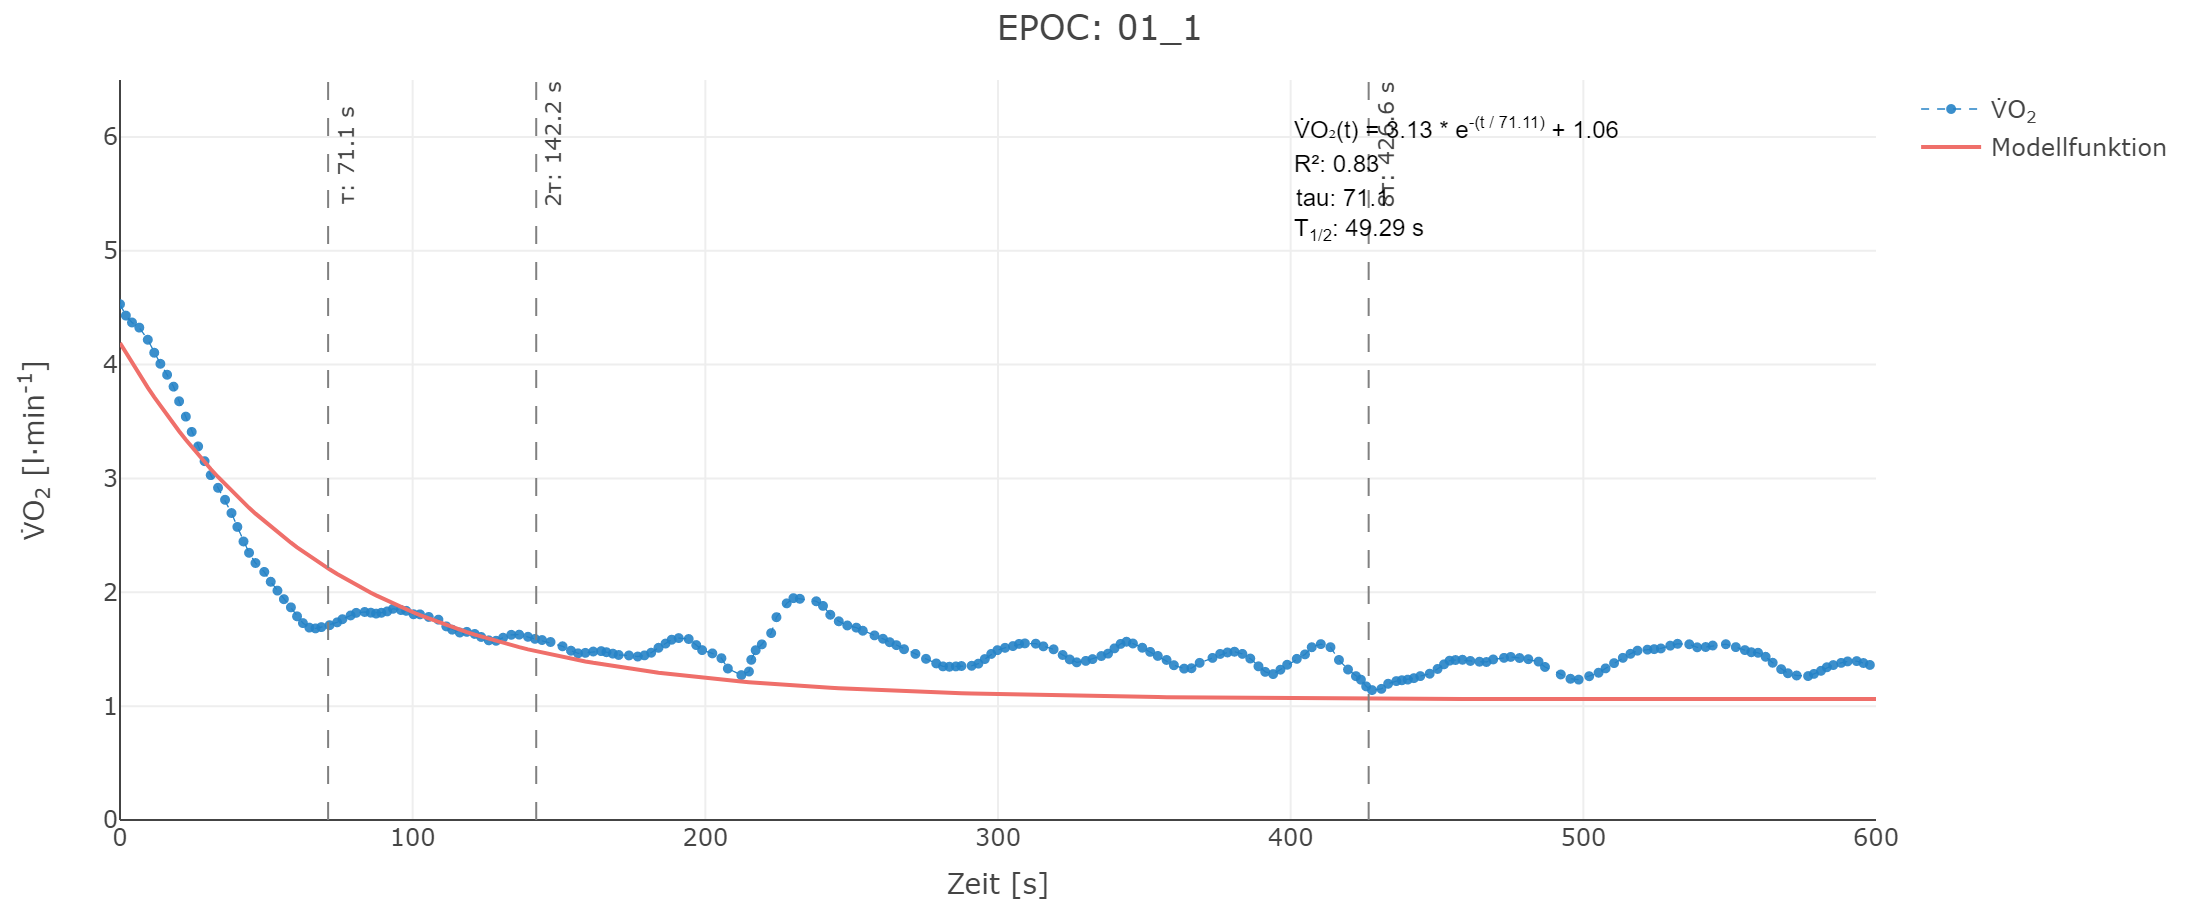
\includegraphics[width=11.45833in,height=4.6875in]{images/01_1_tau.png}
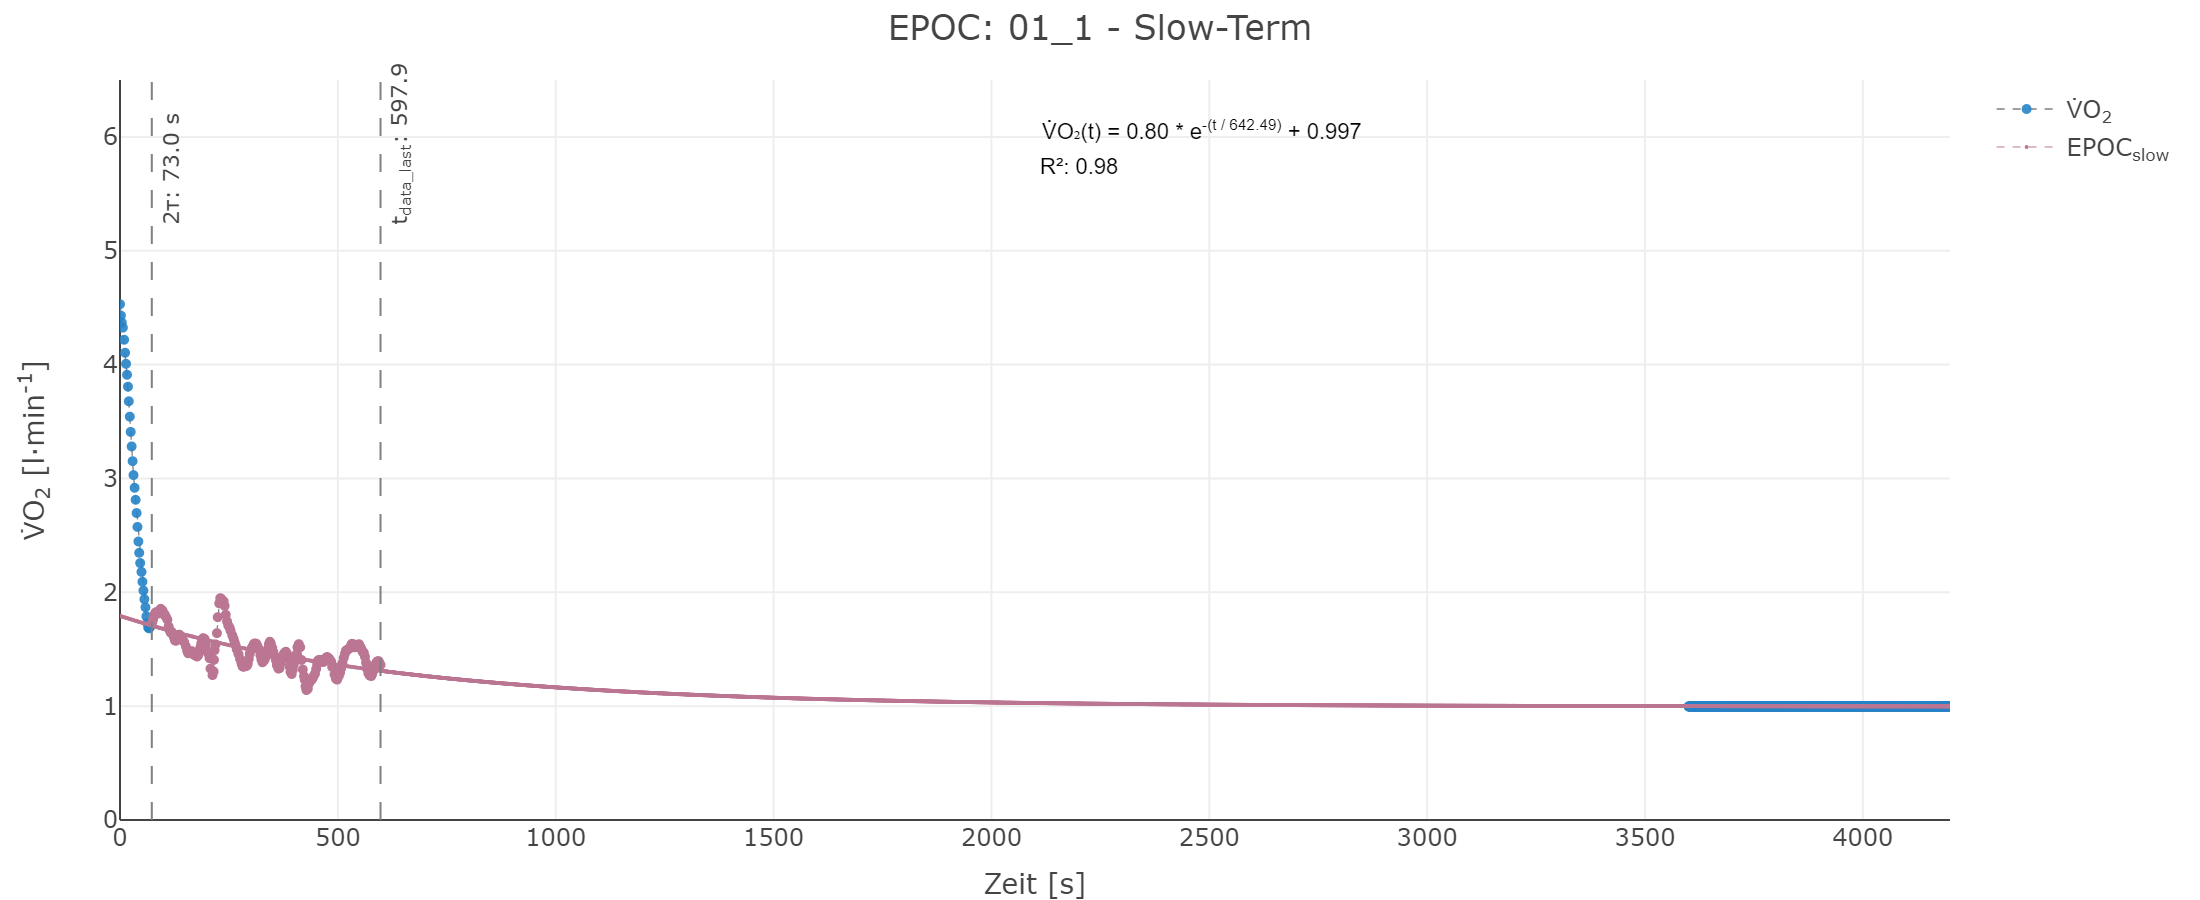
\includegraphics[width=11.45833in,height=4.6875in]{images/01_1_slow.png}
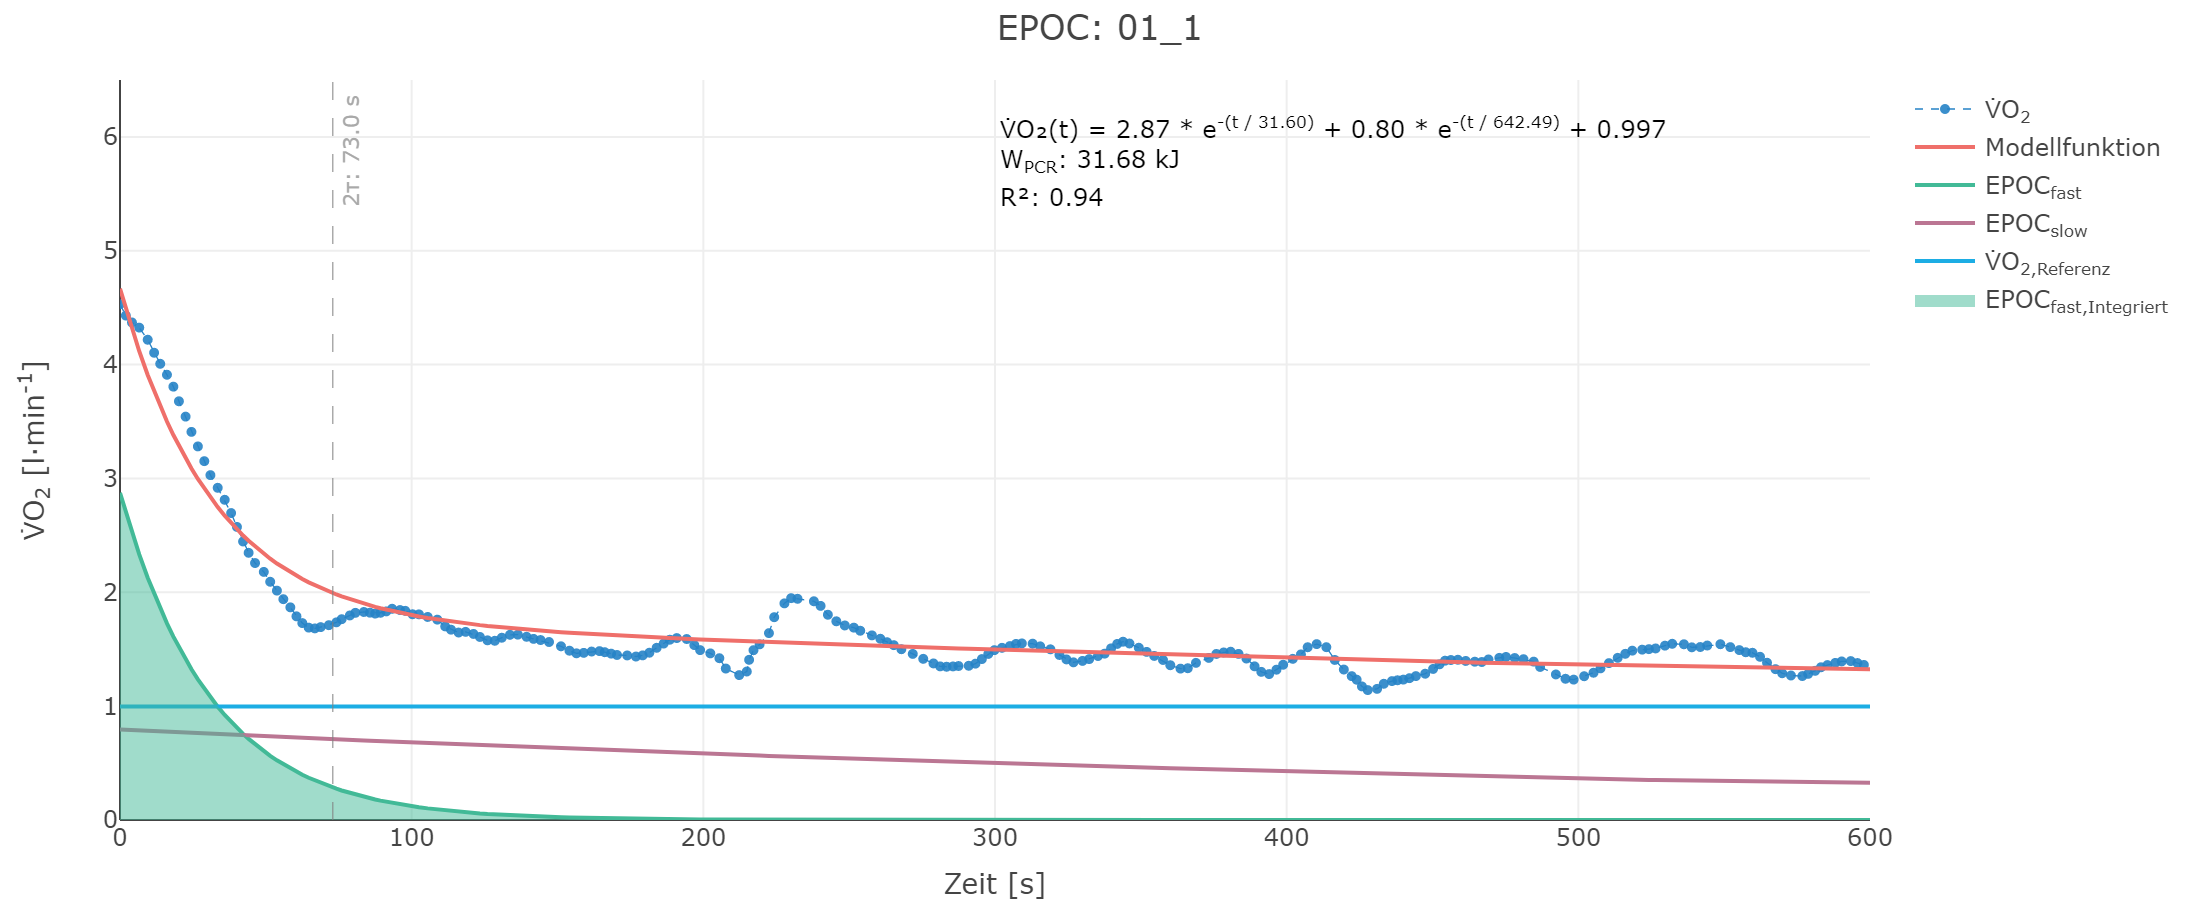
\includegraphics[width=11.45833in,height=4.6875in]{images/01_1.png}

\subsubsection{Test 2}

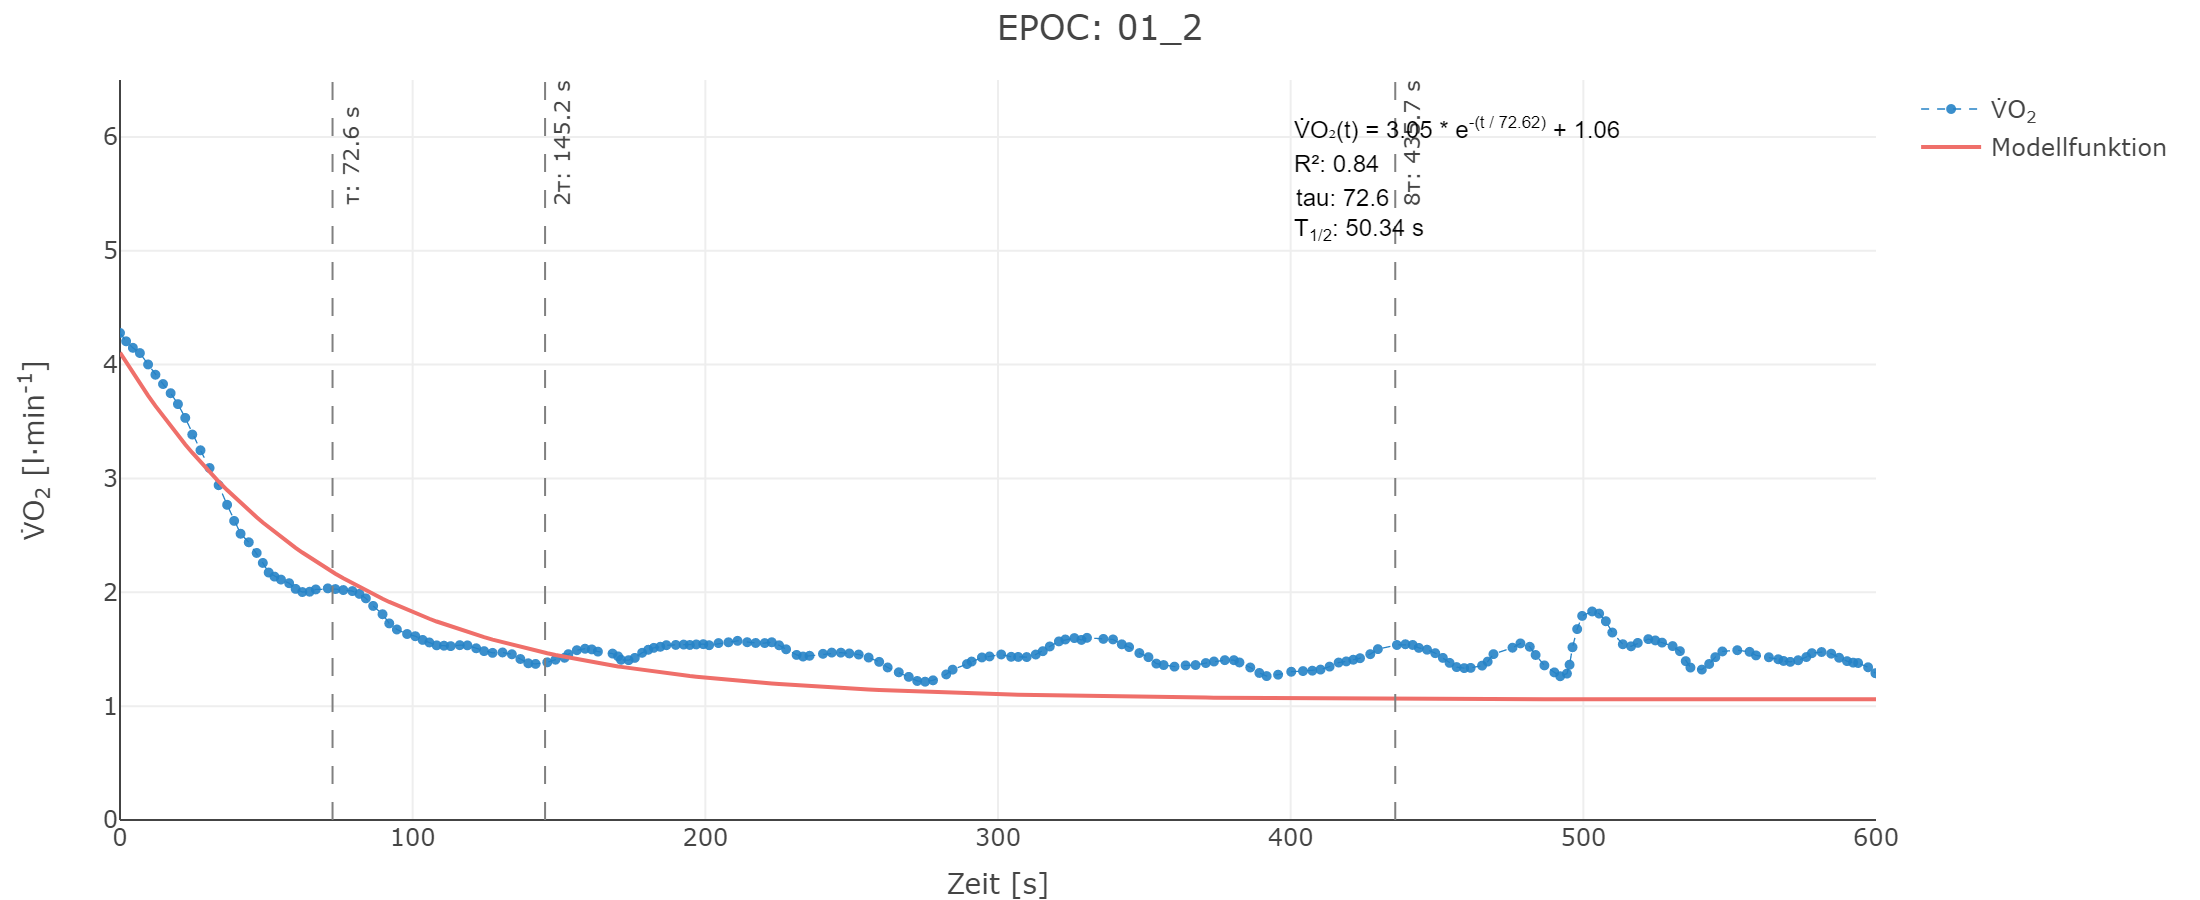
\includegraphics[width=11.45833in,height=4.6875in]{images/01_2_tau.png}
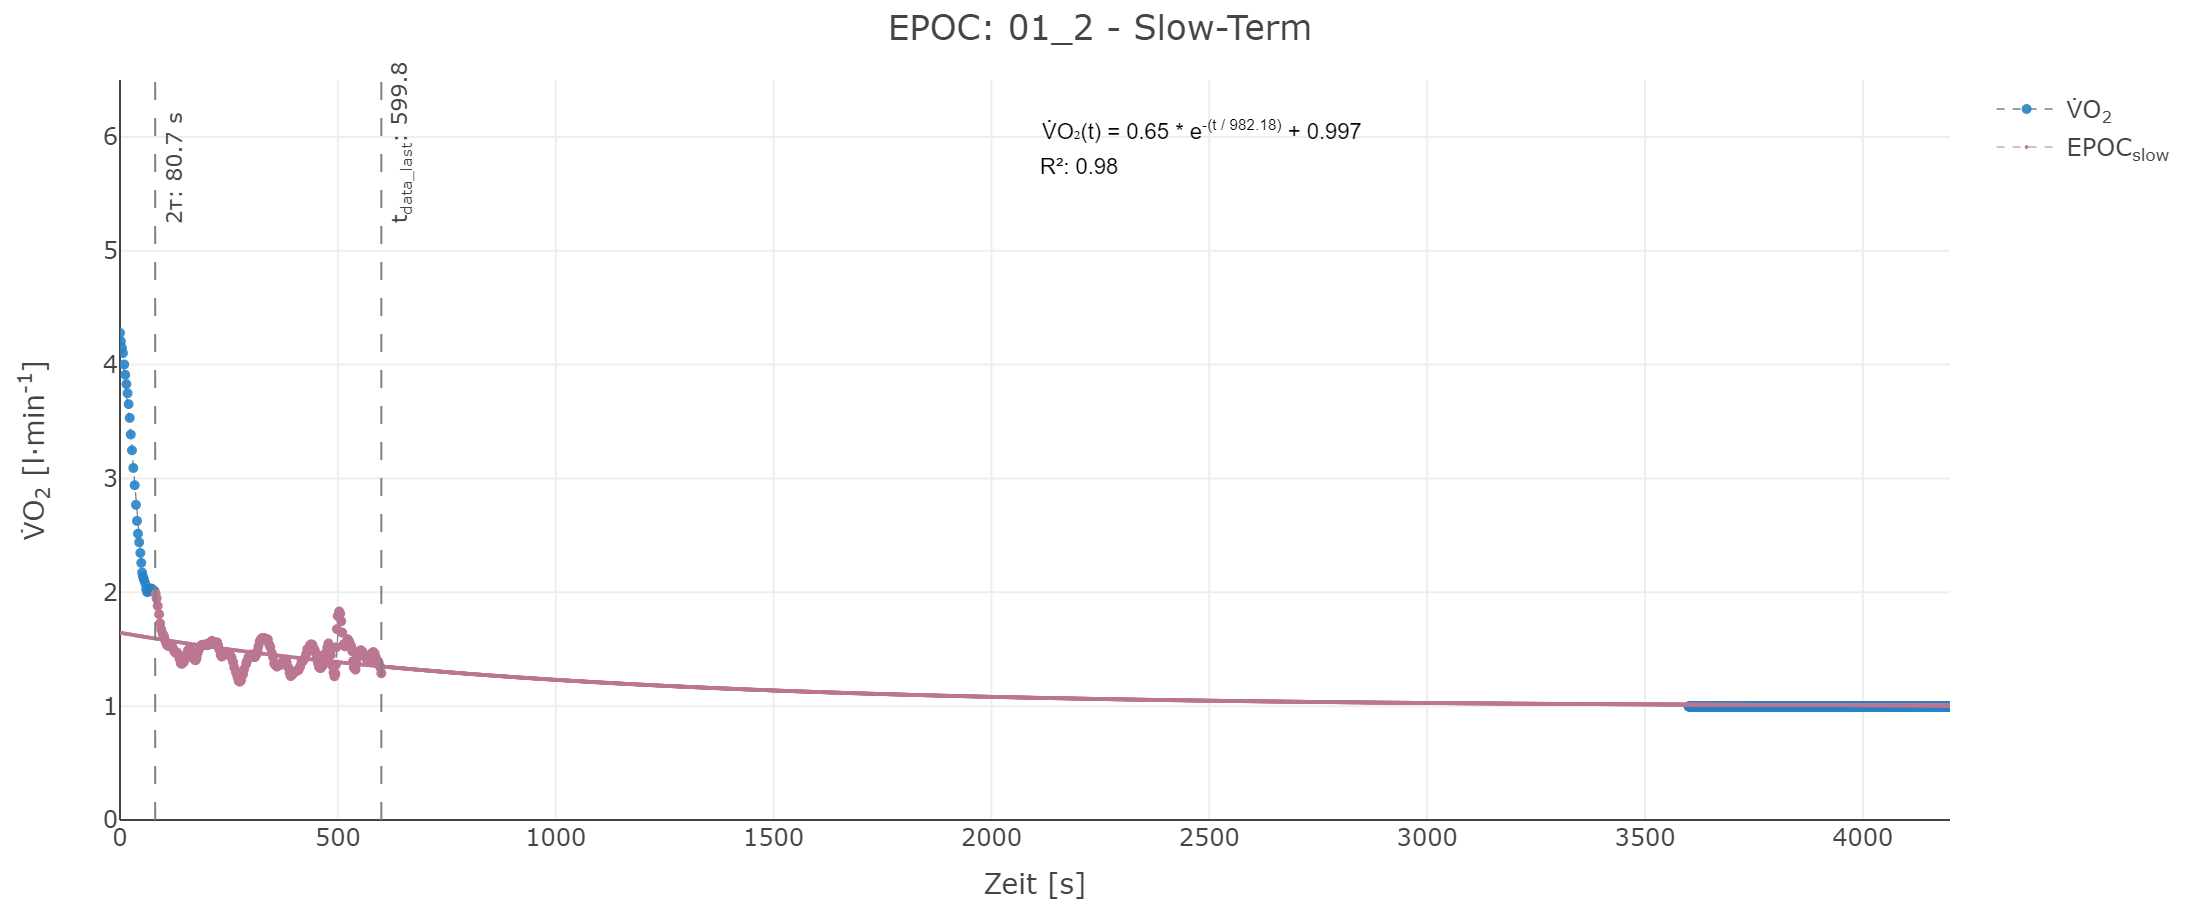
\includegraphics[width=11.45833in,height=4.6875in]{images/01_2_slow.png}
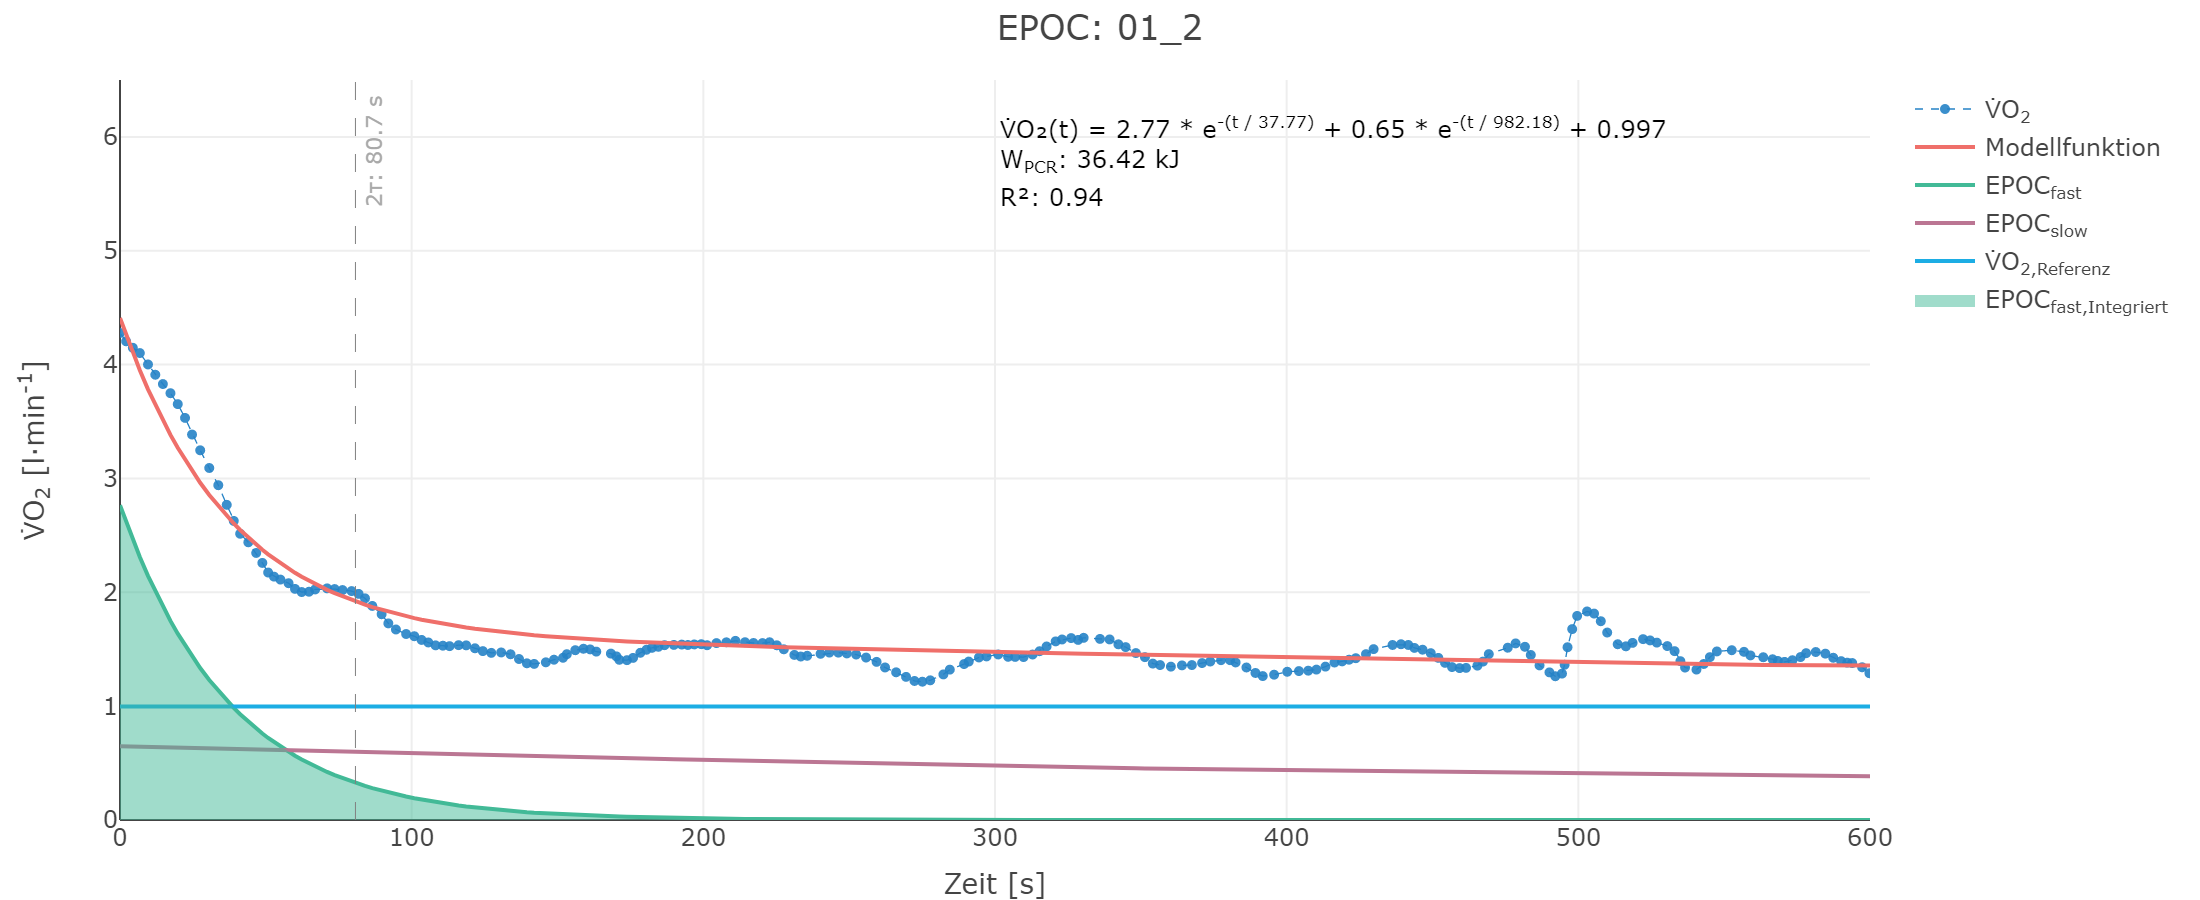
\includegraphics[width=11.45833in,height=4.6875in]{images/01_2.png}

\subsubsection{Test 3}

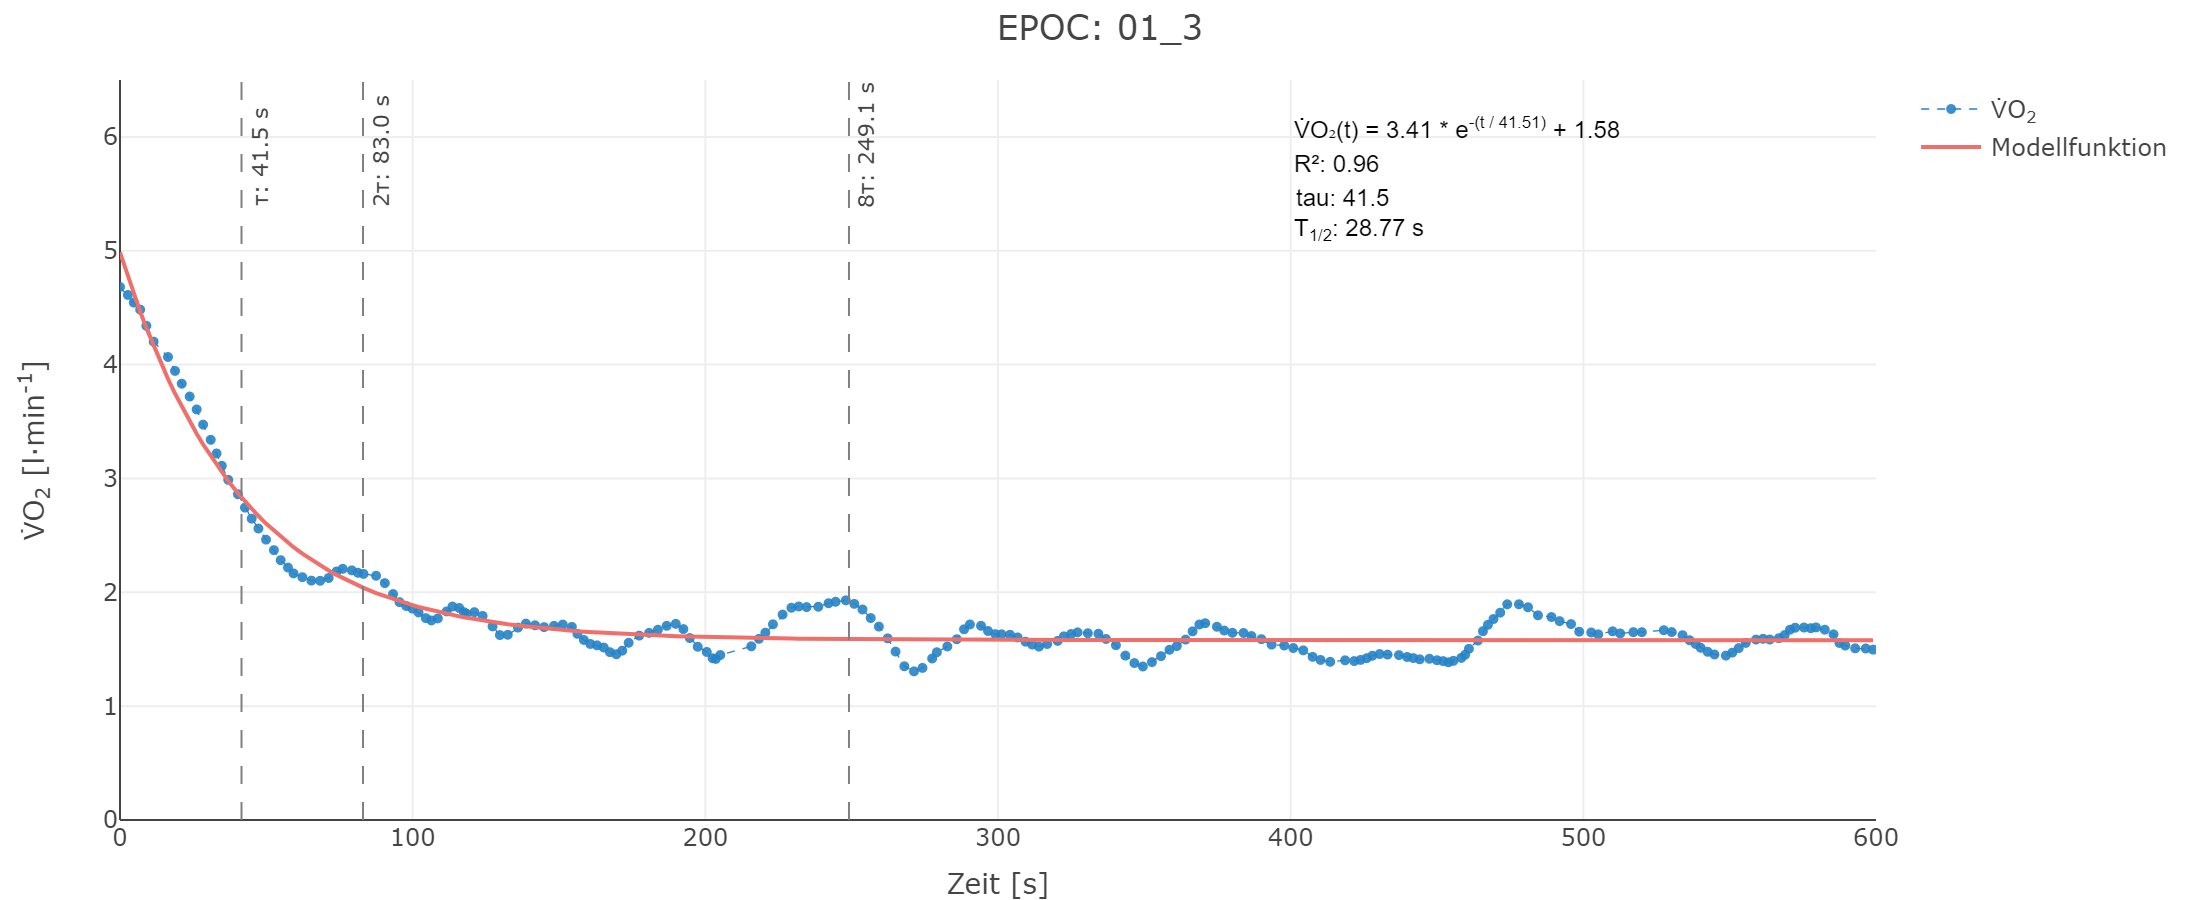
\includegraphics[width=11.45833in,height=4.6875in]{images/01_3_tau.png}
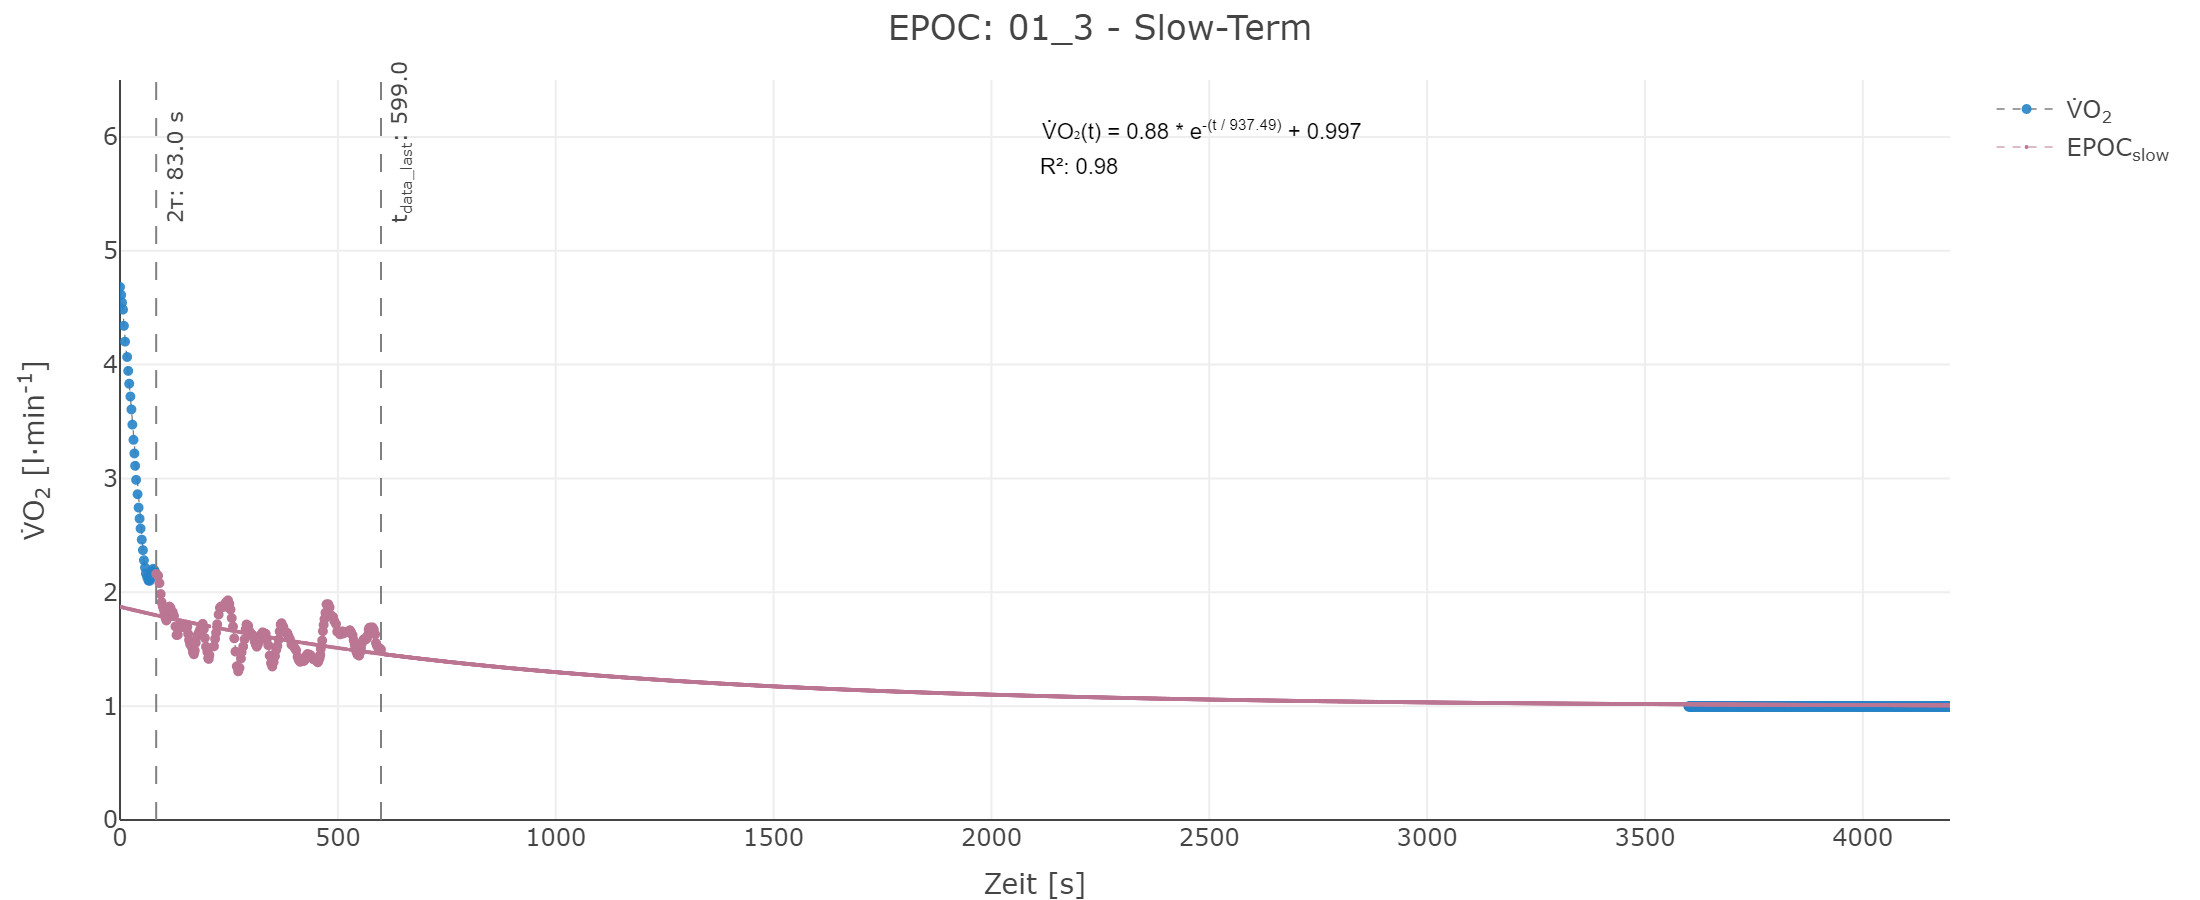
\includegraphics[width=11.45833in,height=4.6875in]{images/01_3_slow.png}
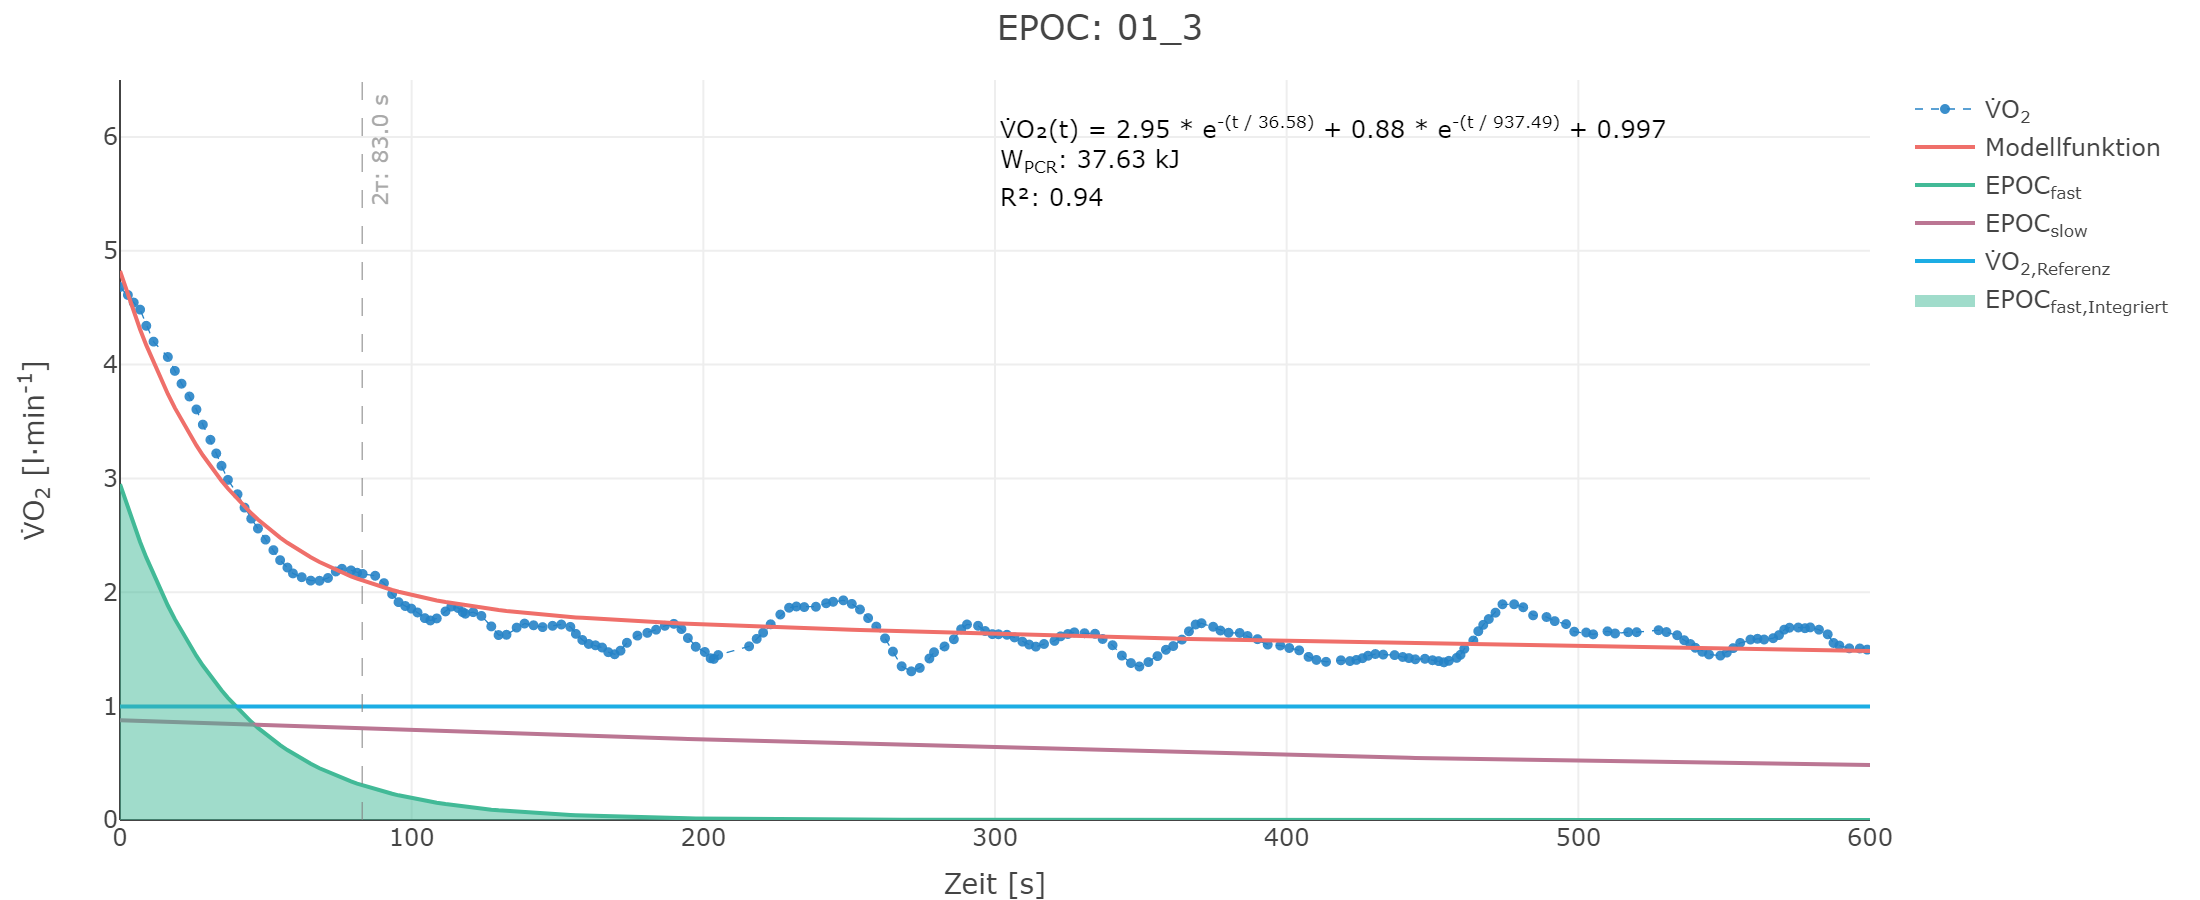
\includegraphics[width=11.45833in,height=4.6875in]{images/01_3.png}

\subsubsection{Test 4}

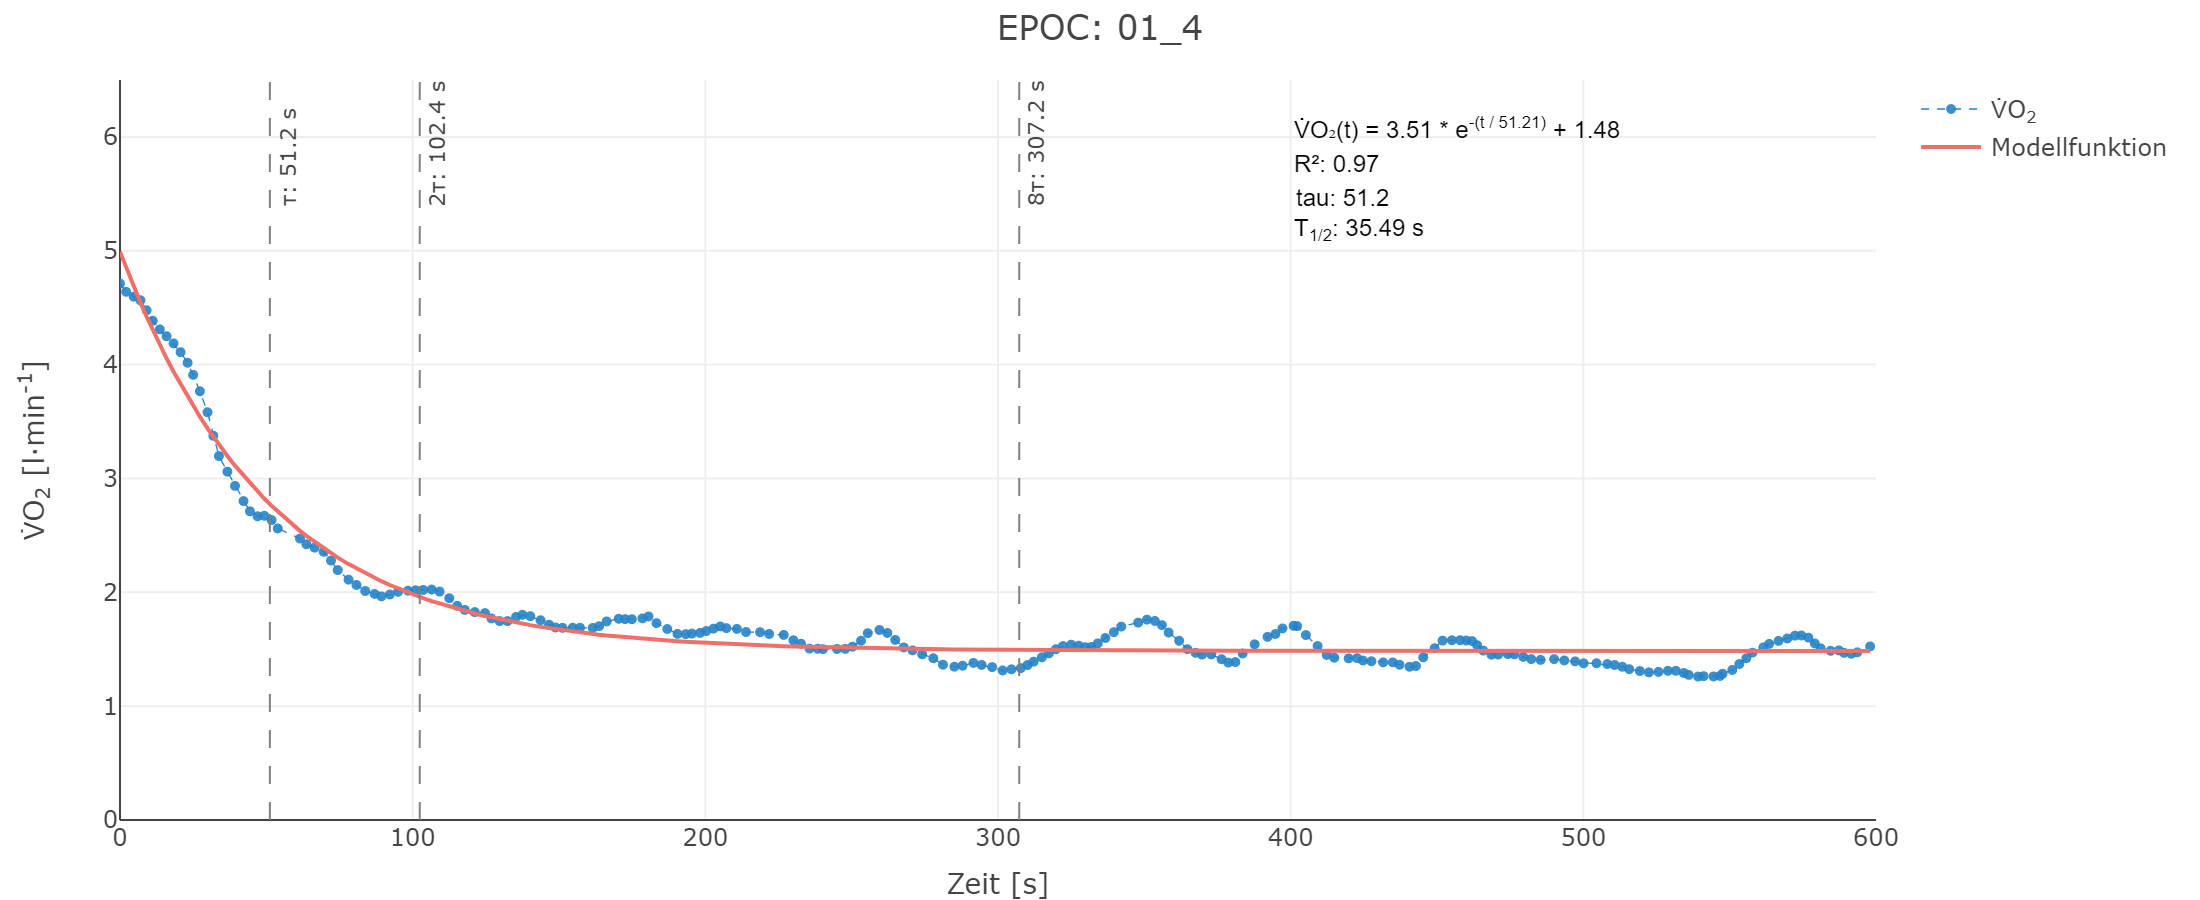
\includegraphics[width=11.45833in,height=4.6875in]{images/01_4_tau.png}
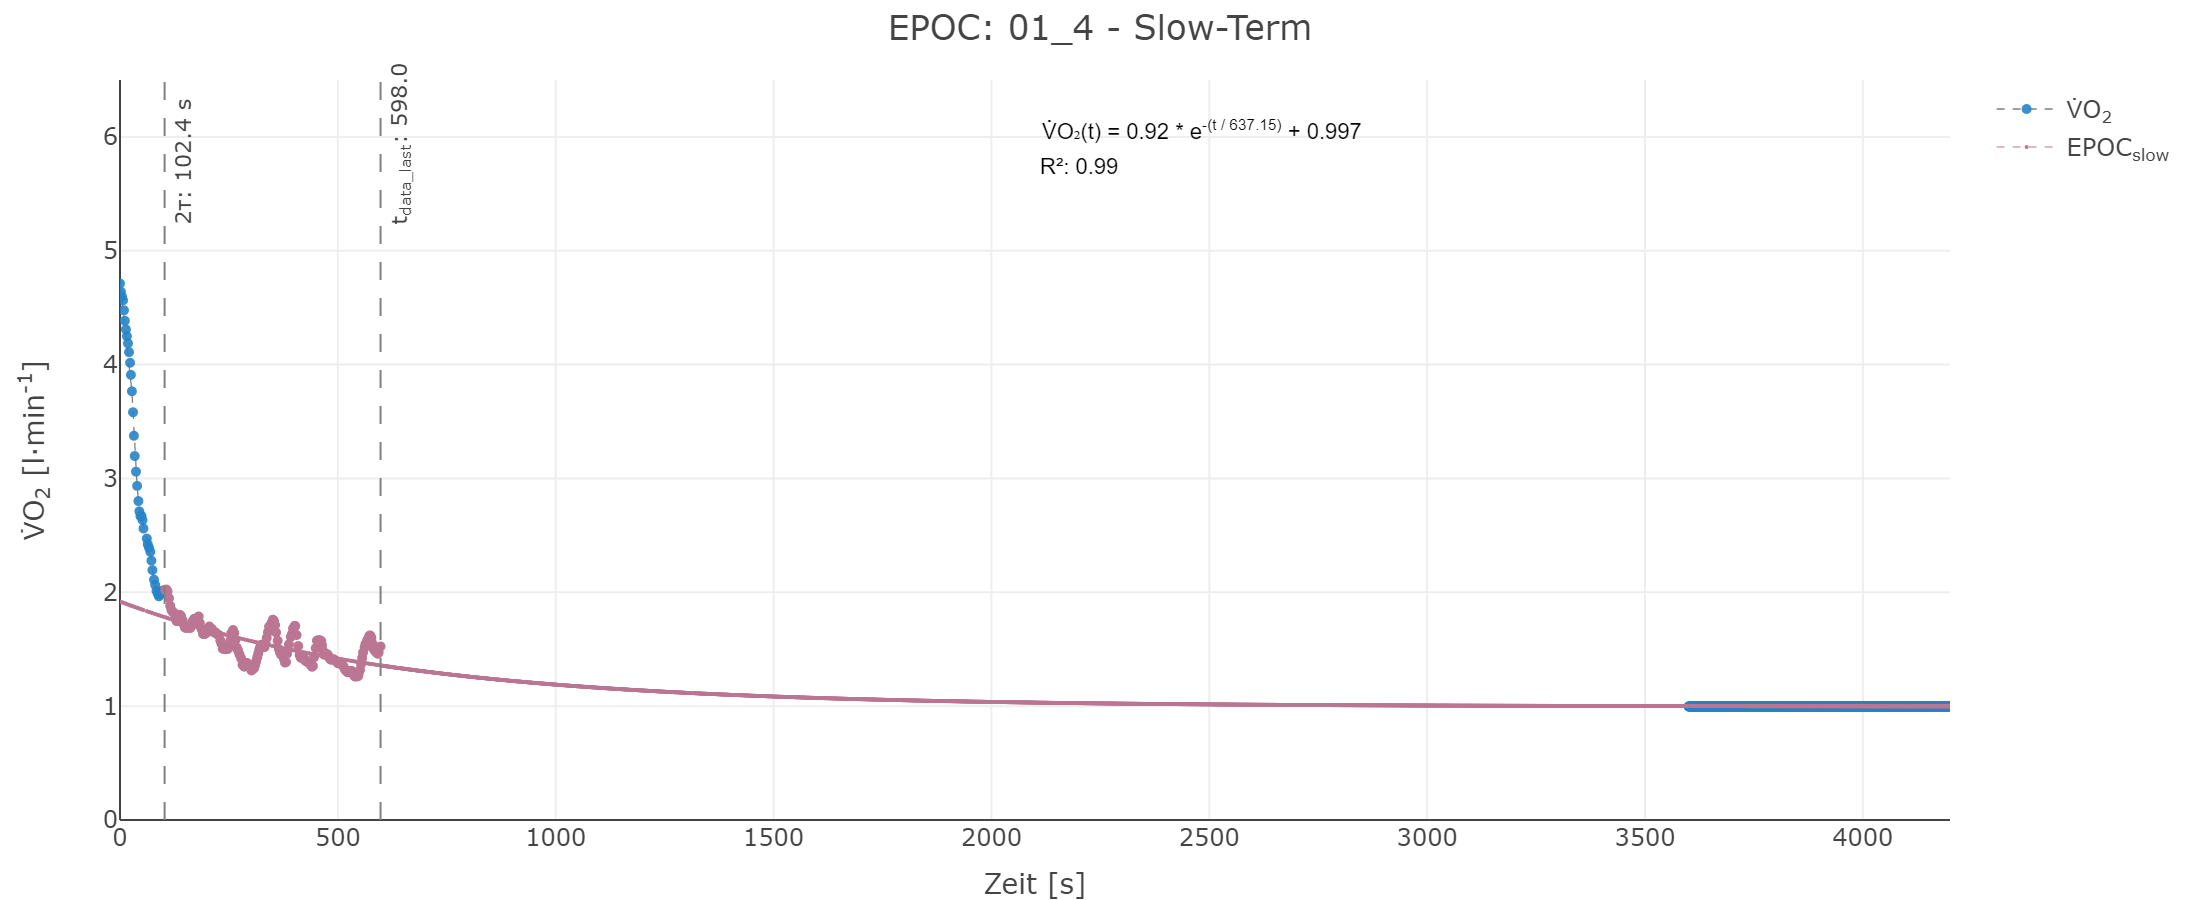
\includegraphics[width=11.45833in,height=4.6875in]{images/01_4_slow.png}
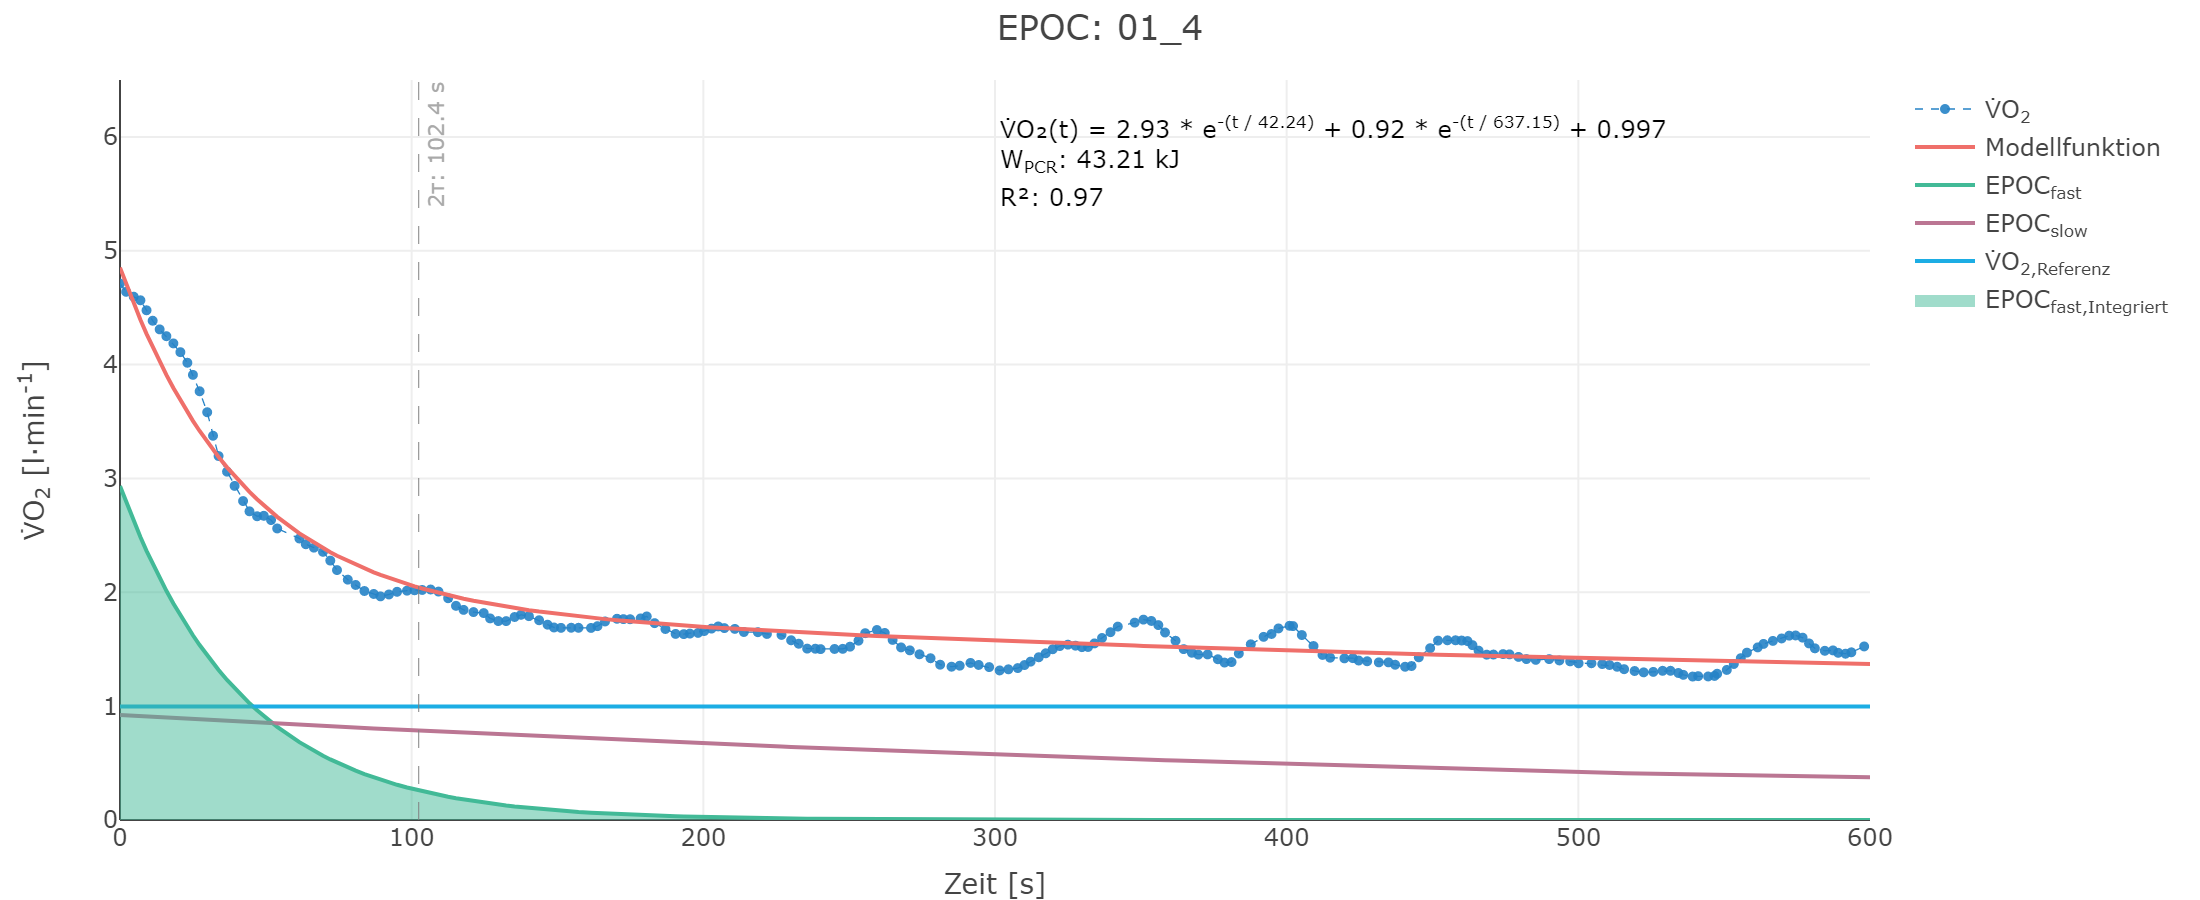
\includegraphics[width=11.45833in,height=4.6875in]{images/01_4.png}

\subsubsection{Test 5}

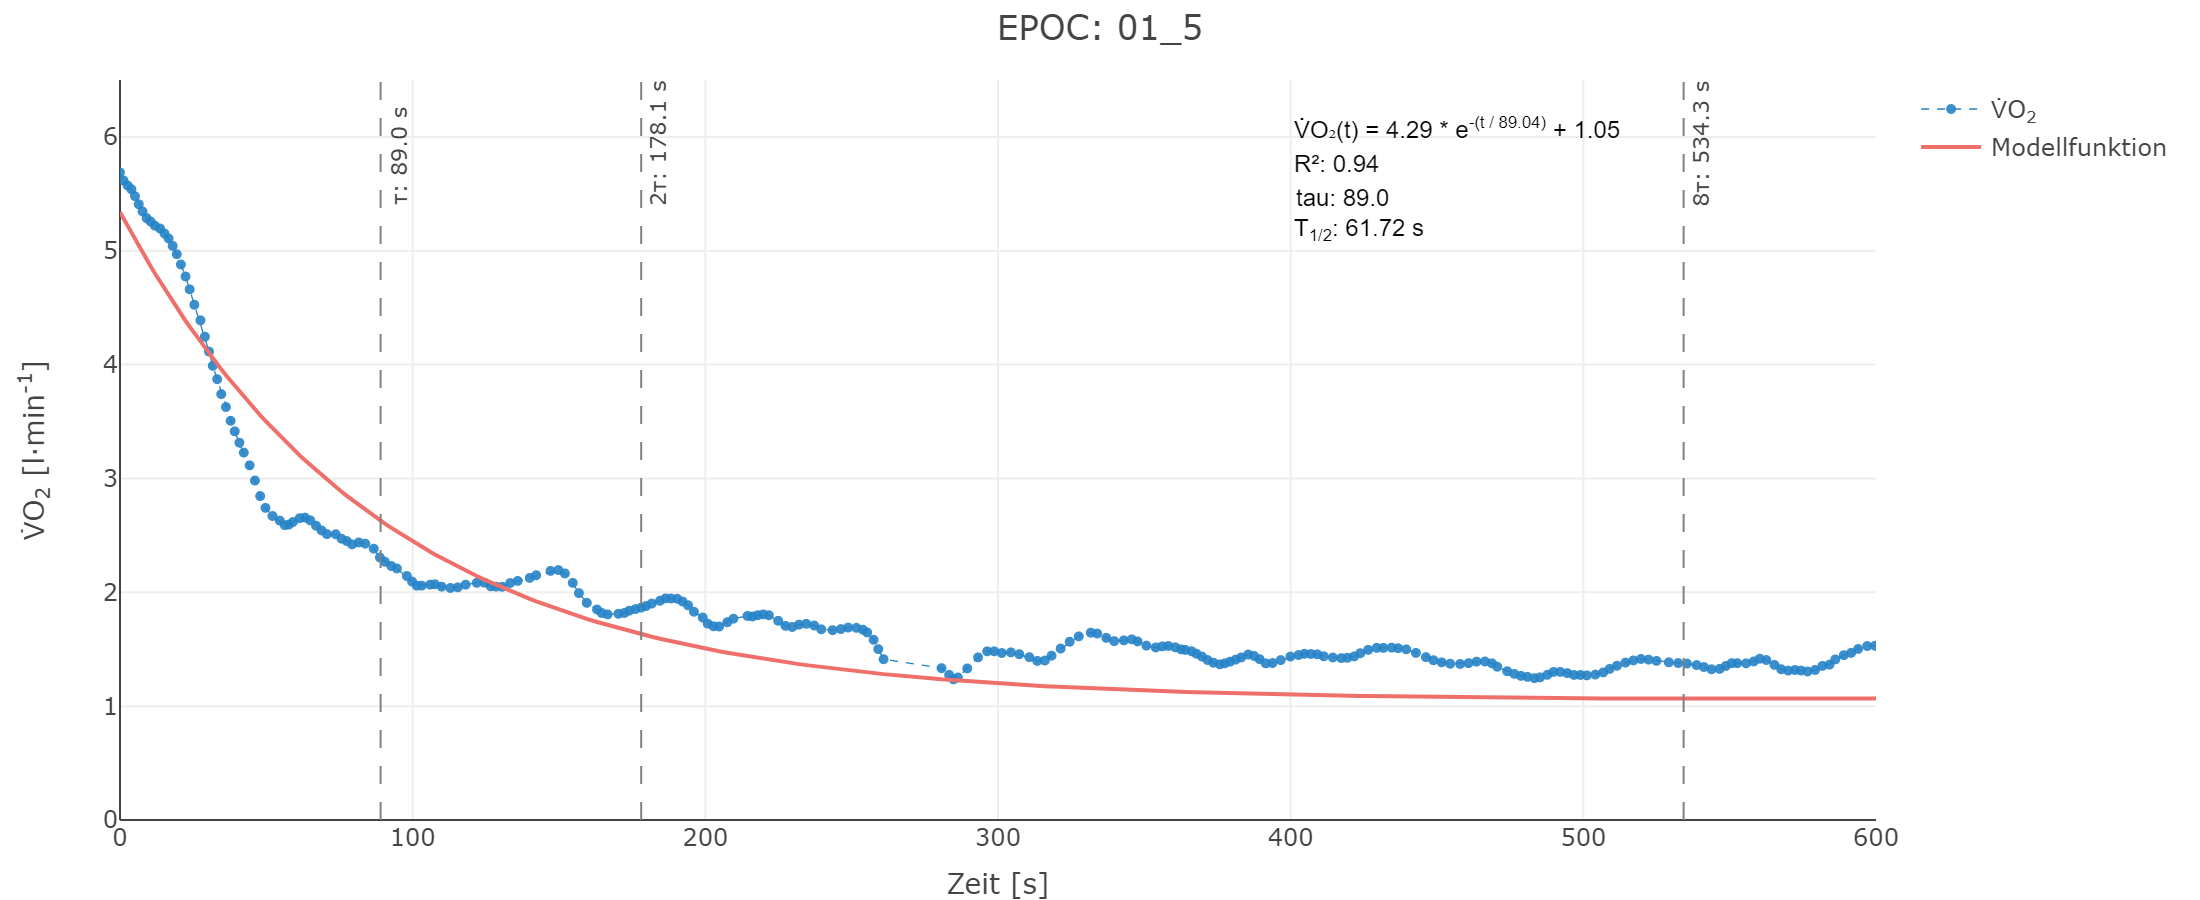
\includegraphics[width=11.45833in,height=4.6875in]{images/01_5_tau.png}
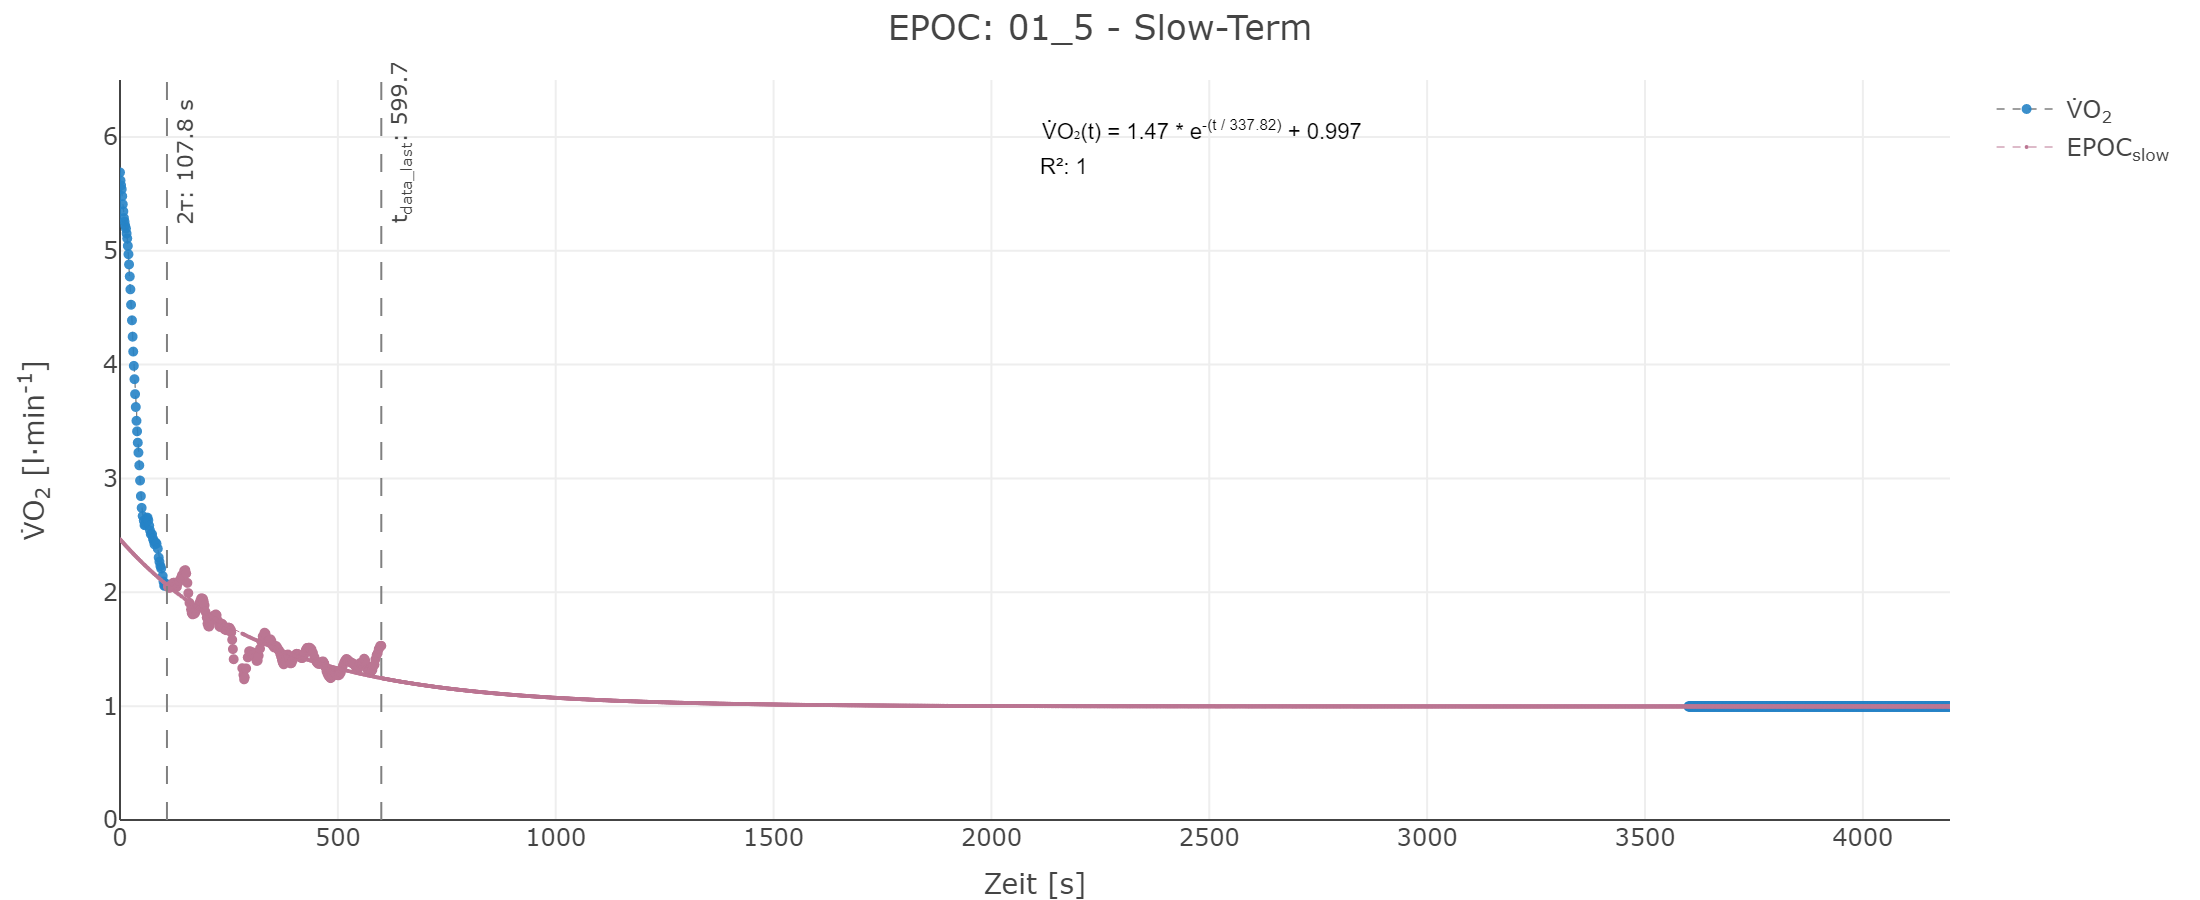
\includegraphics[width=11.45833in,height=4.6875in]{images/01_5_slow.png}
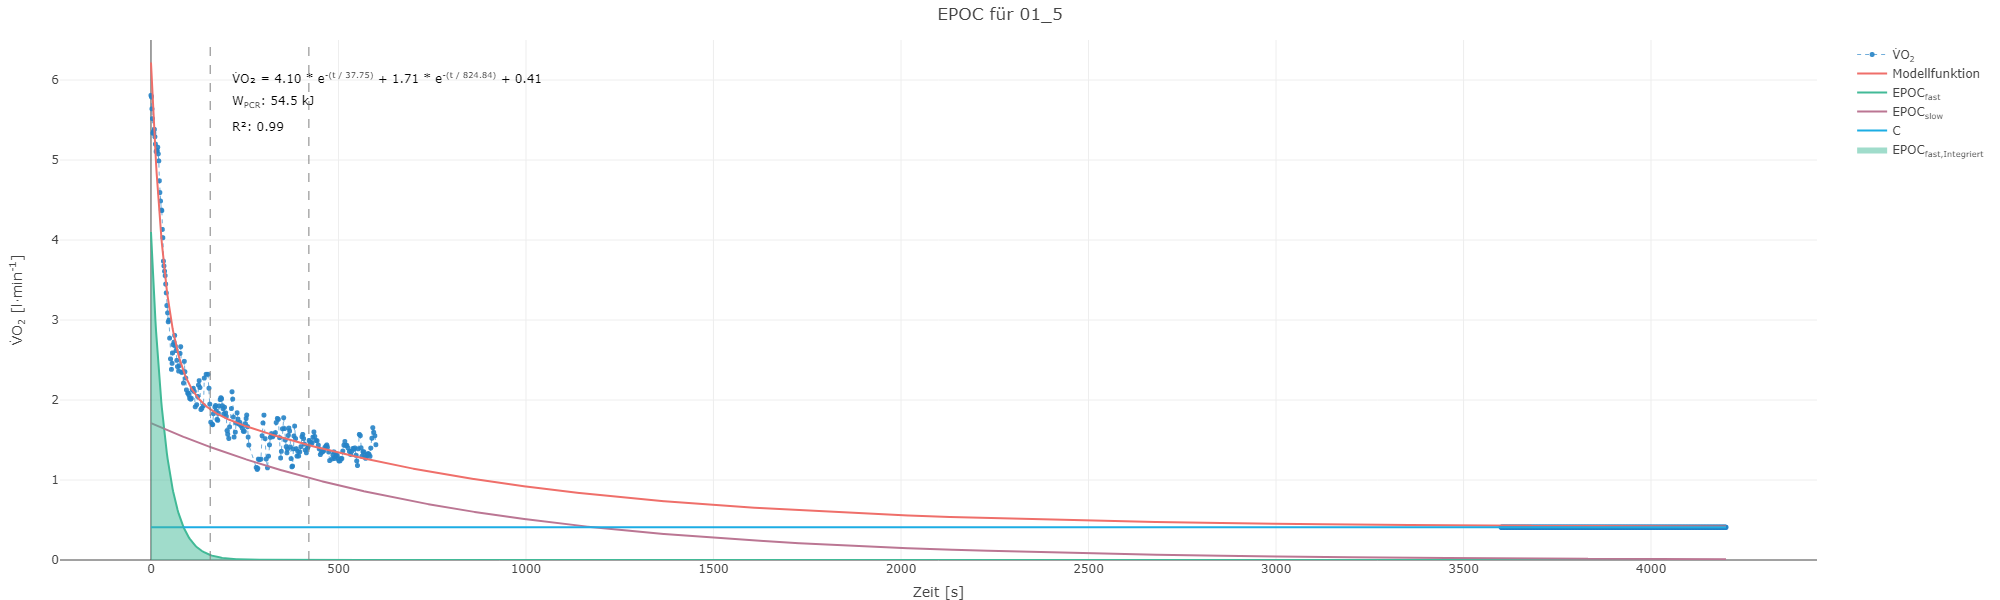
\includegraphics[width=11.45833in,height=4.6875in]{images/01_5.png}

\subsubsection{Test 6}

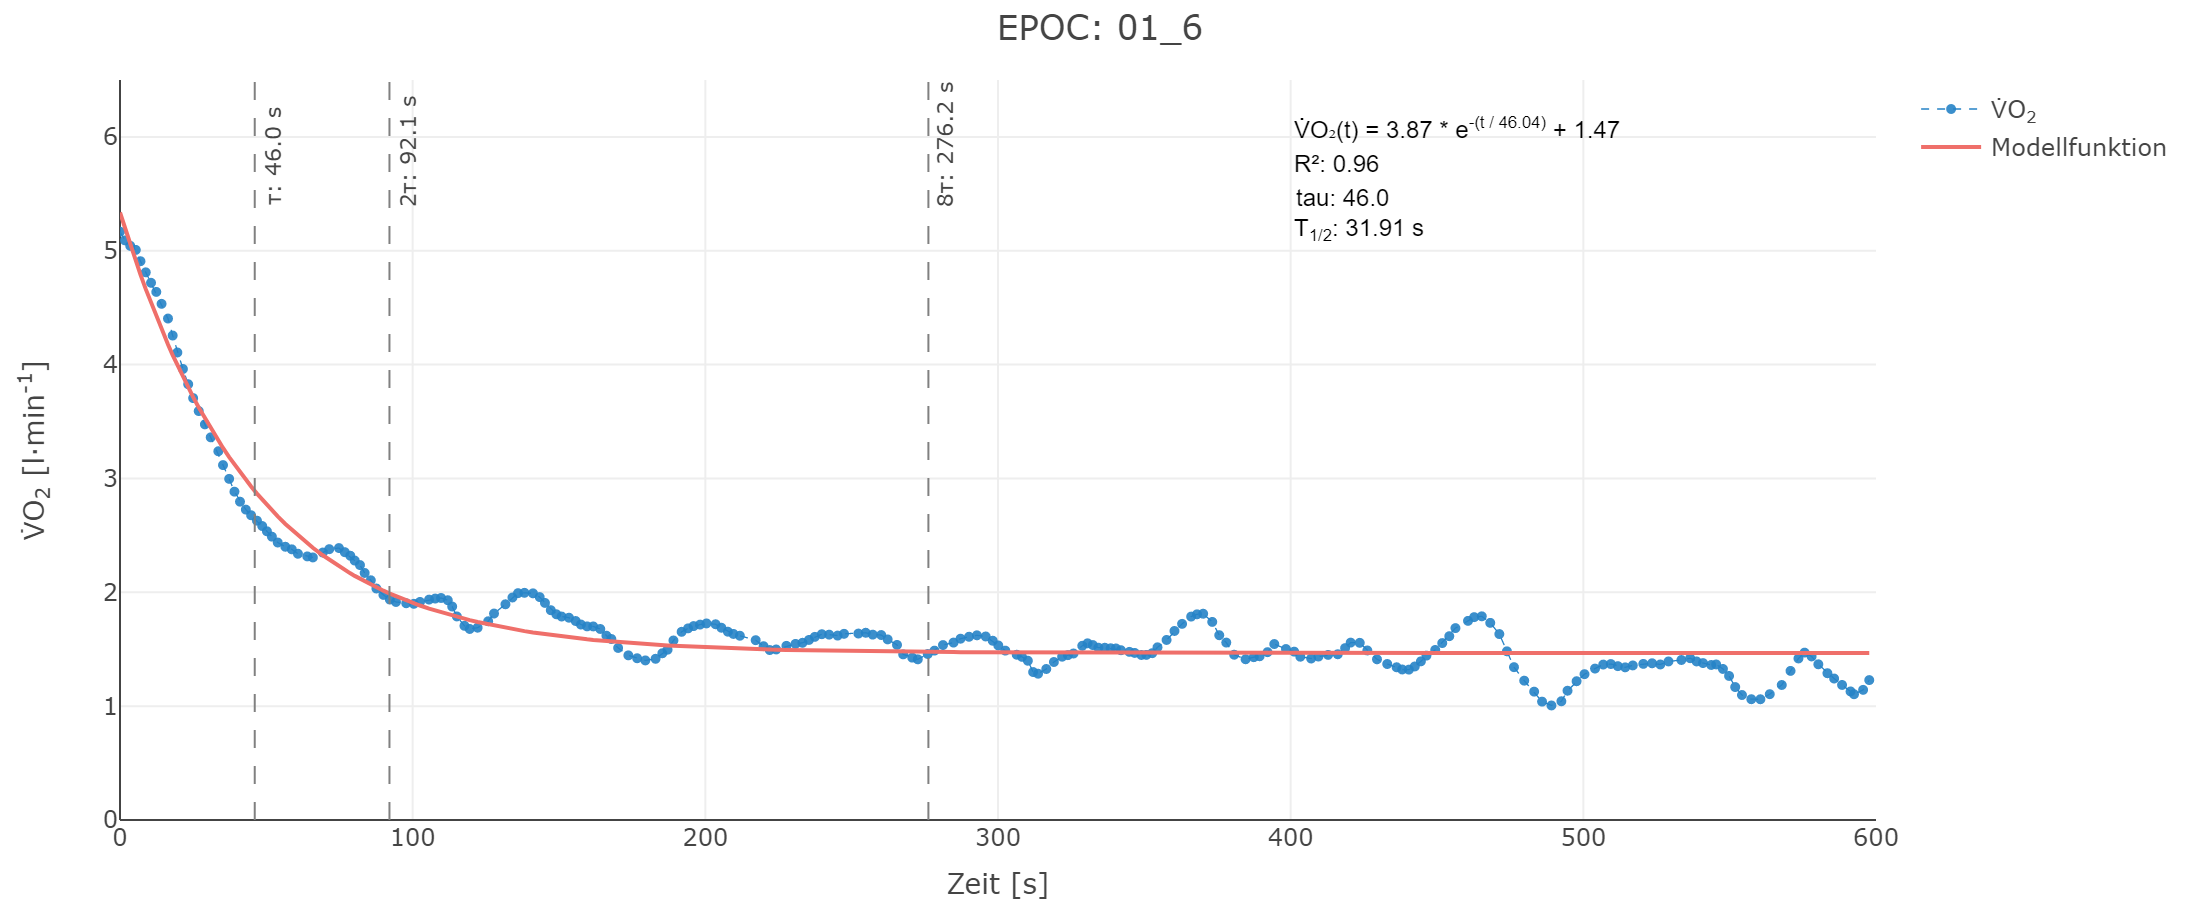
\includegraphics[width=11.45833in,height=4.6875in]{images/01_6_tau.png}
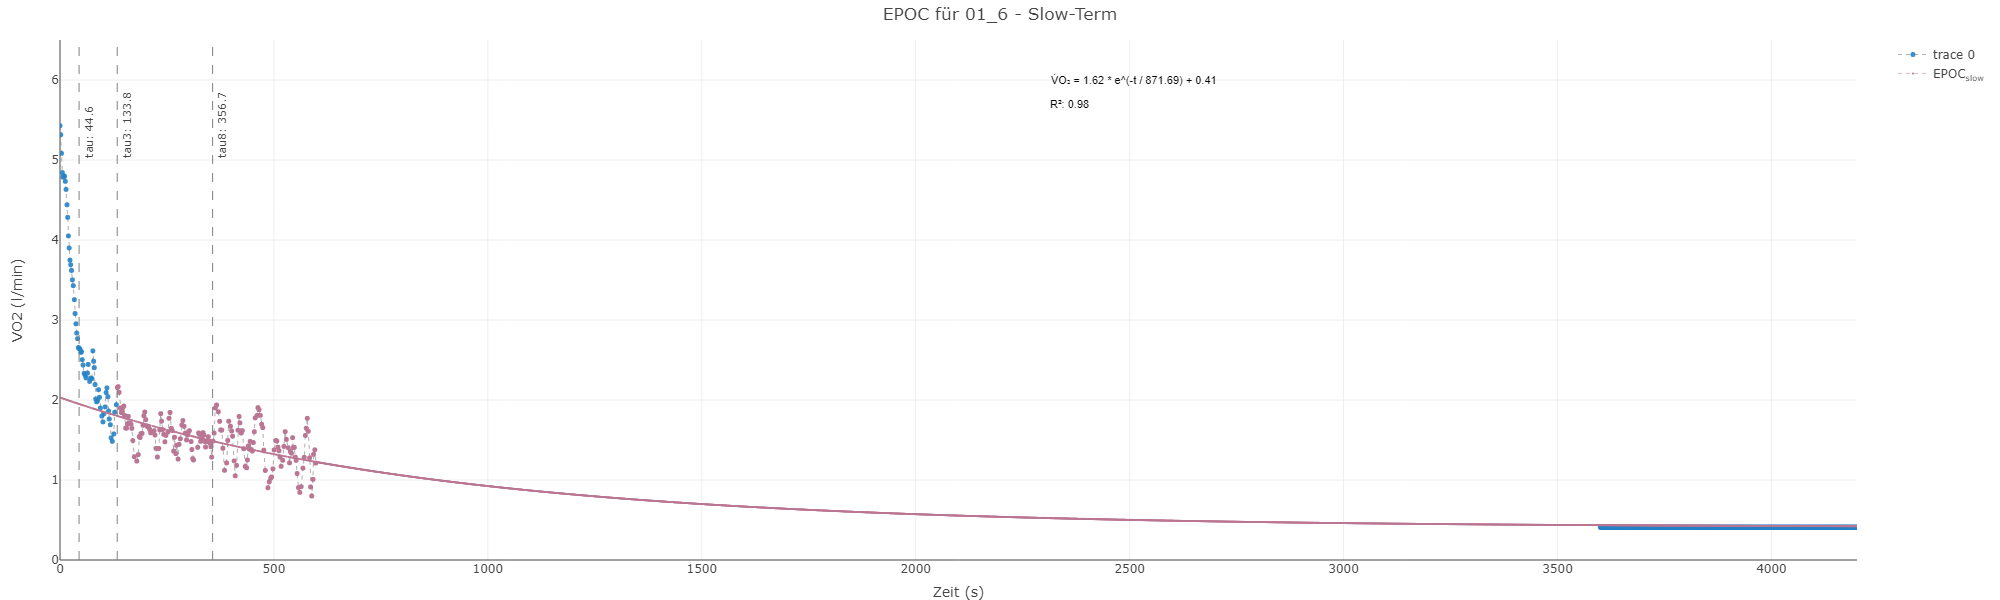
\includegraphics[width=11.45833in,height=4.6875in]{images/01_6_slow.png}
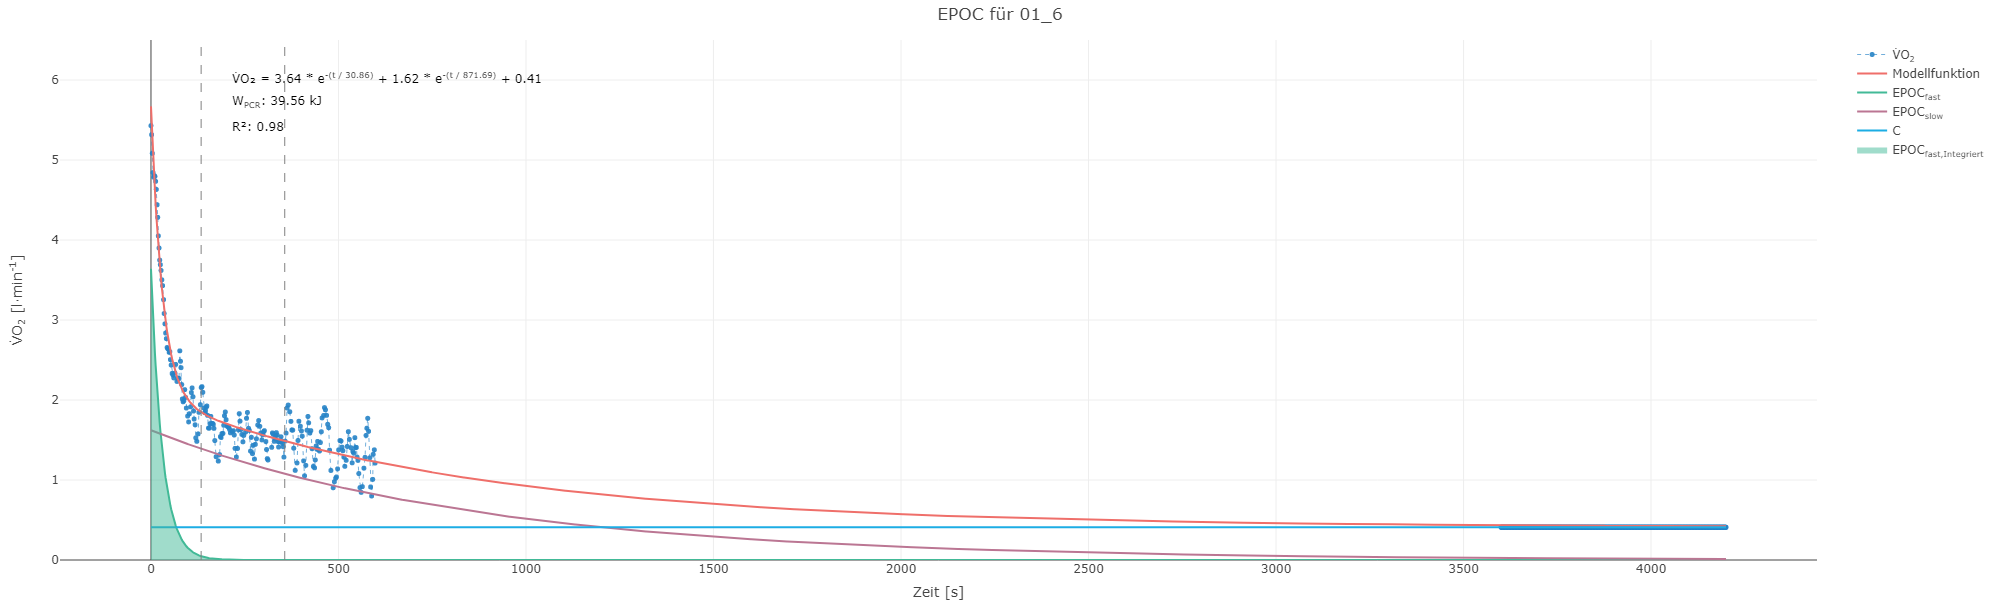
\includegraphics[width=11.45833in,height=4.6875in]{images/01_6.png}

\subsection{Proband 06}

\subsubsection{Test 1}

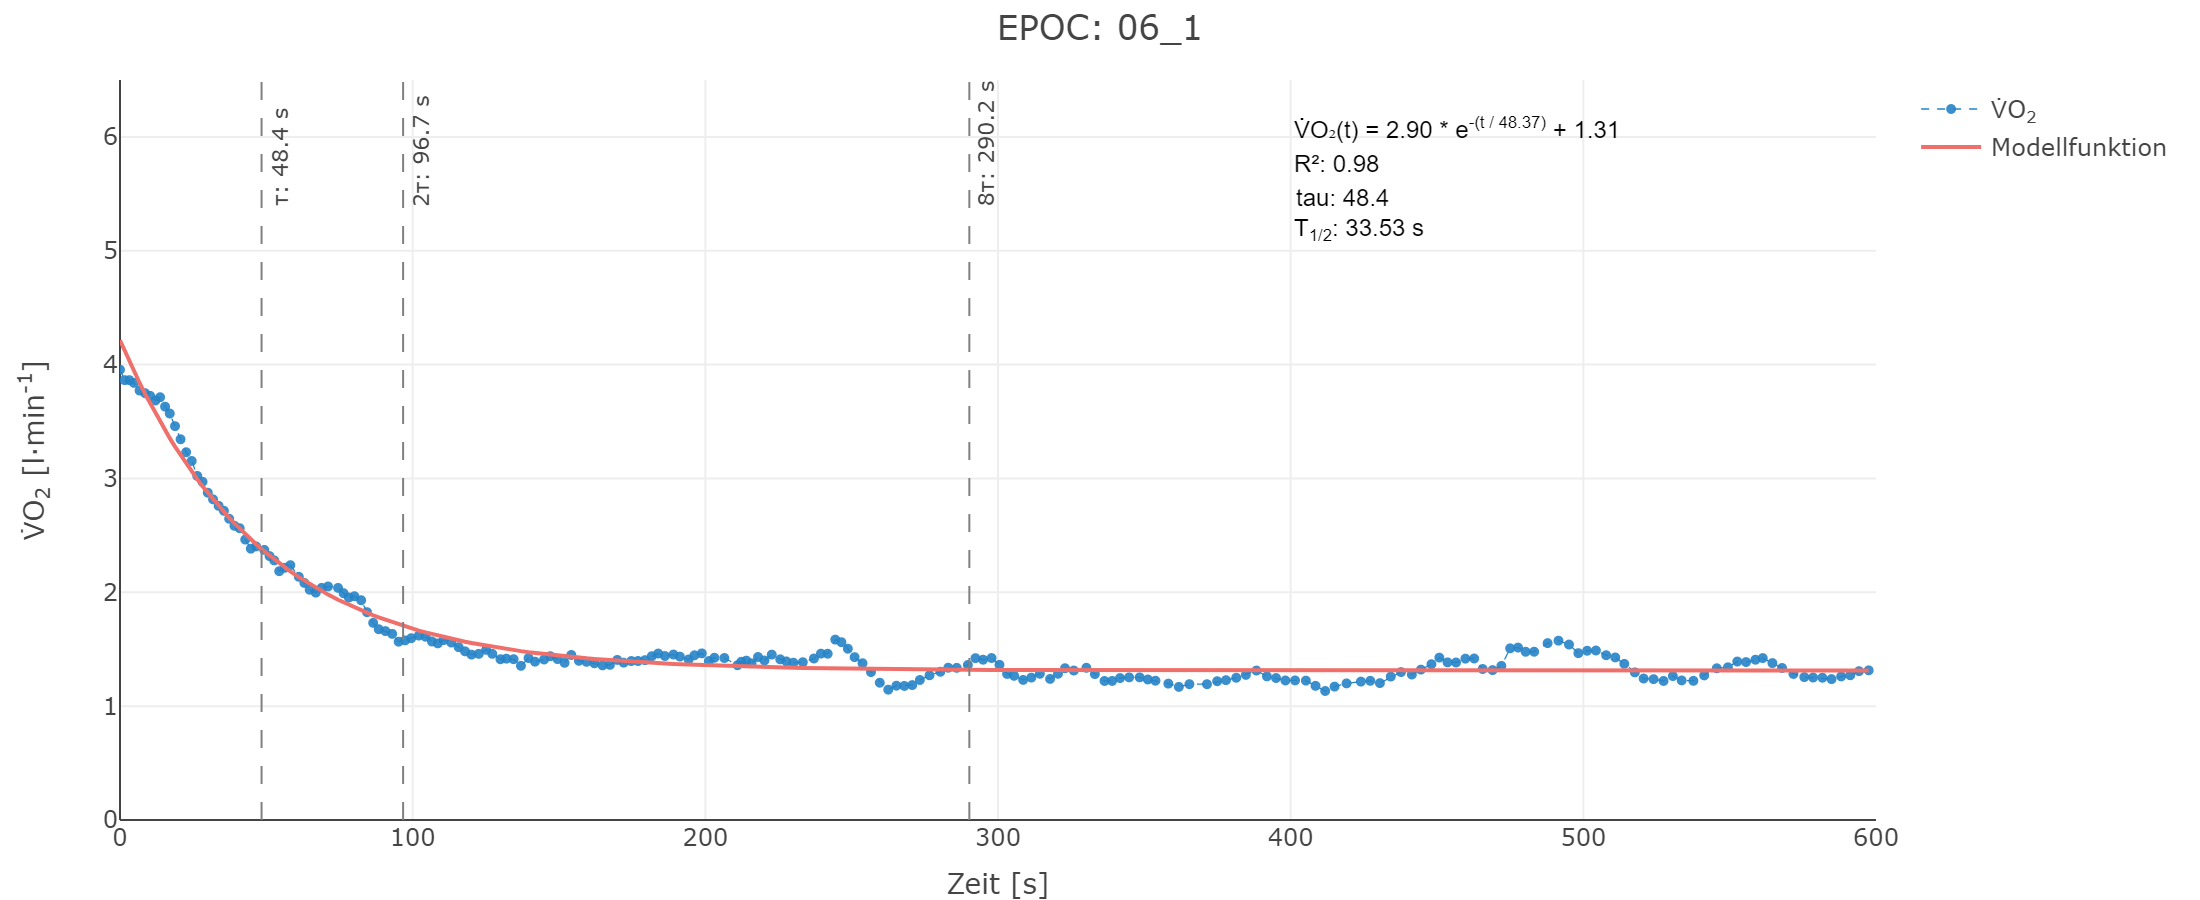
\includegraphics[width=11.45833in,height=4.6875in]{images/06_1_tau.png}
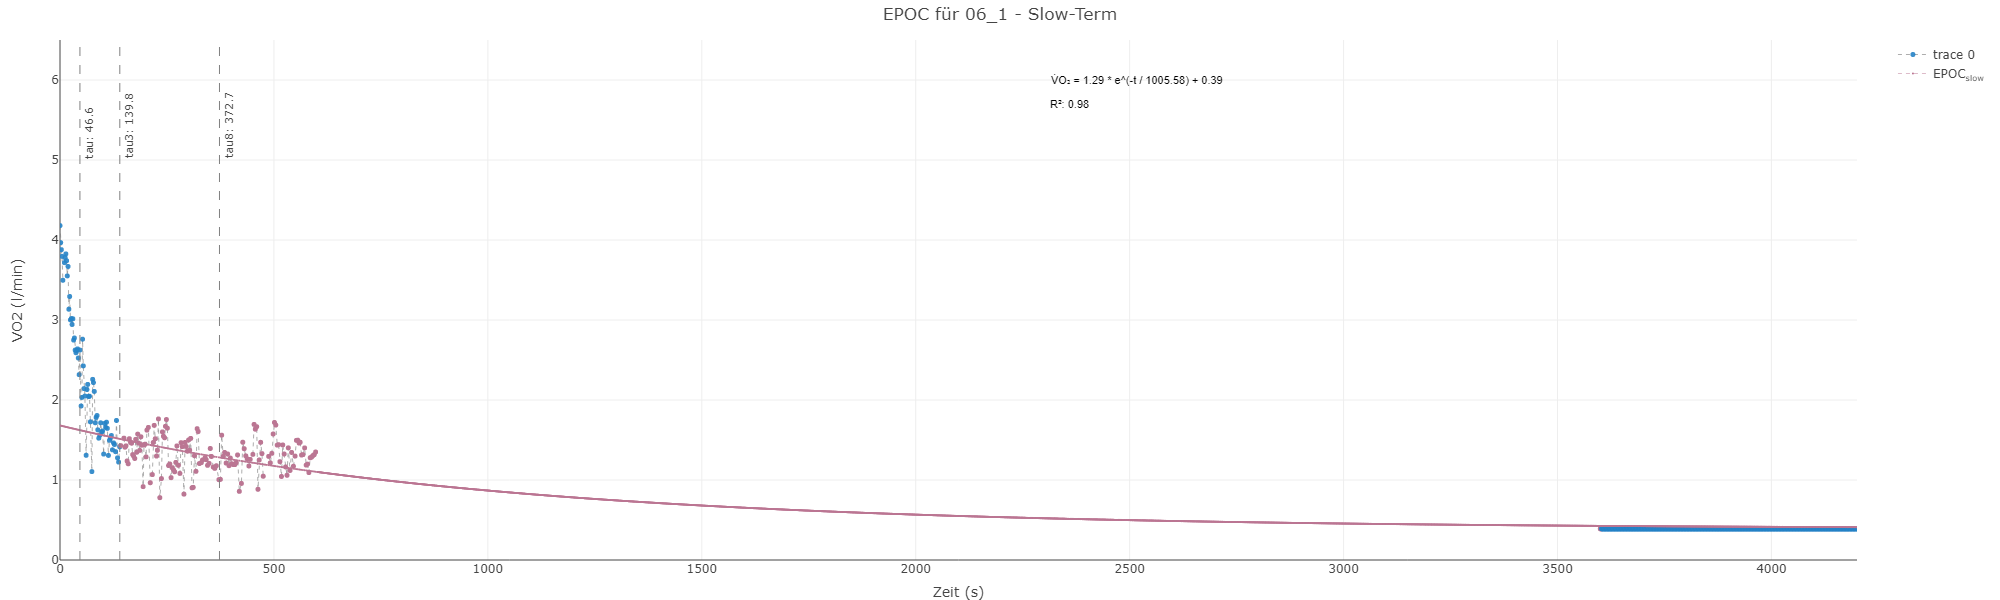
\includegraphics[width=11.45833in,height=4.6875in]{images/06_1_slow.png}
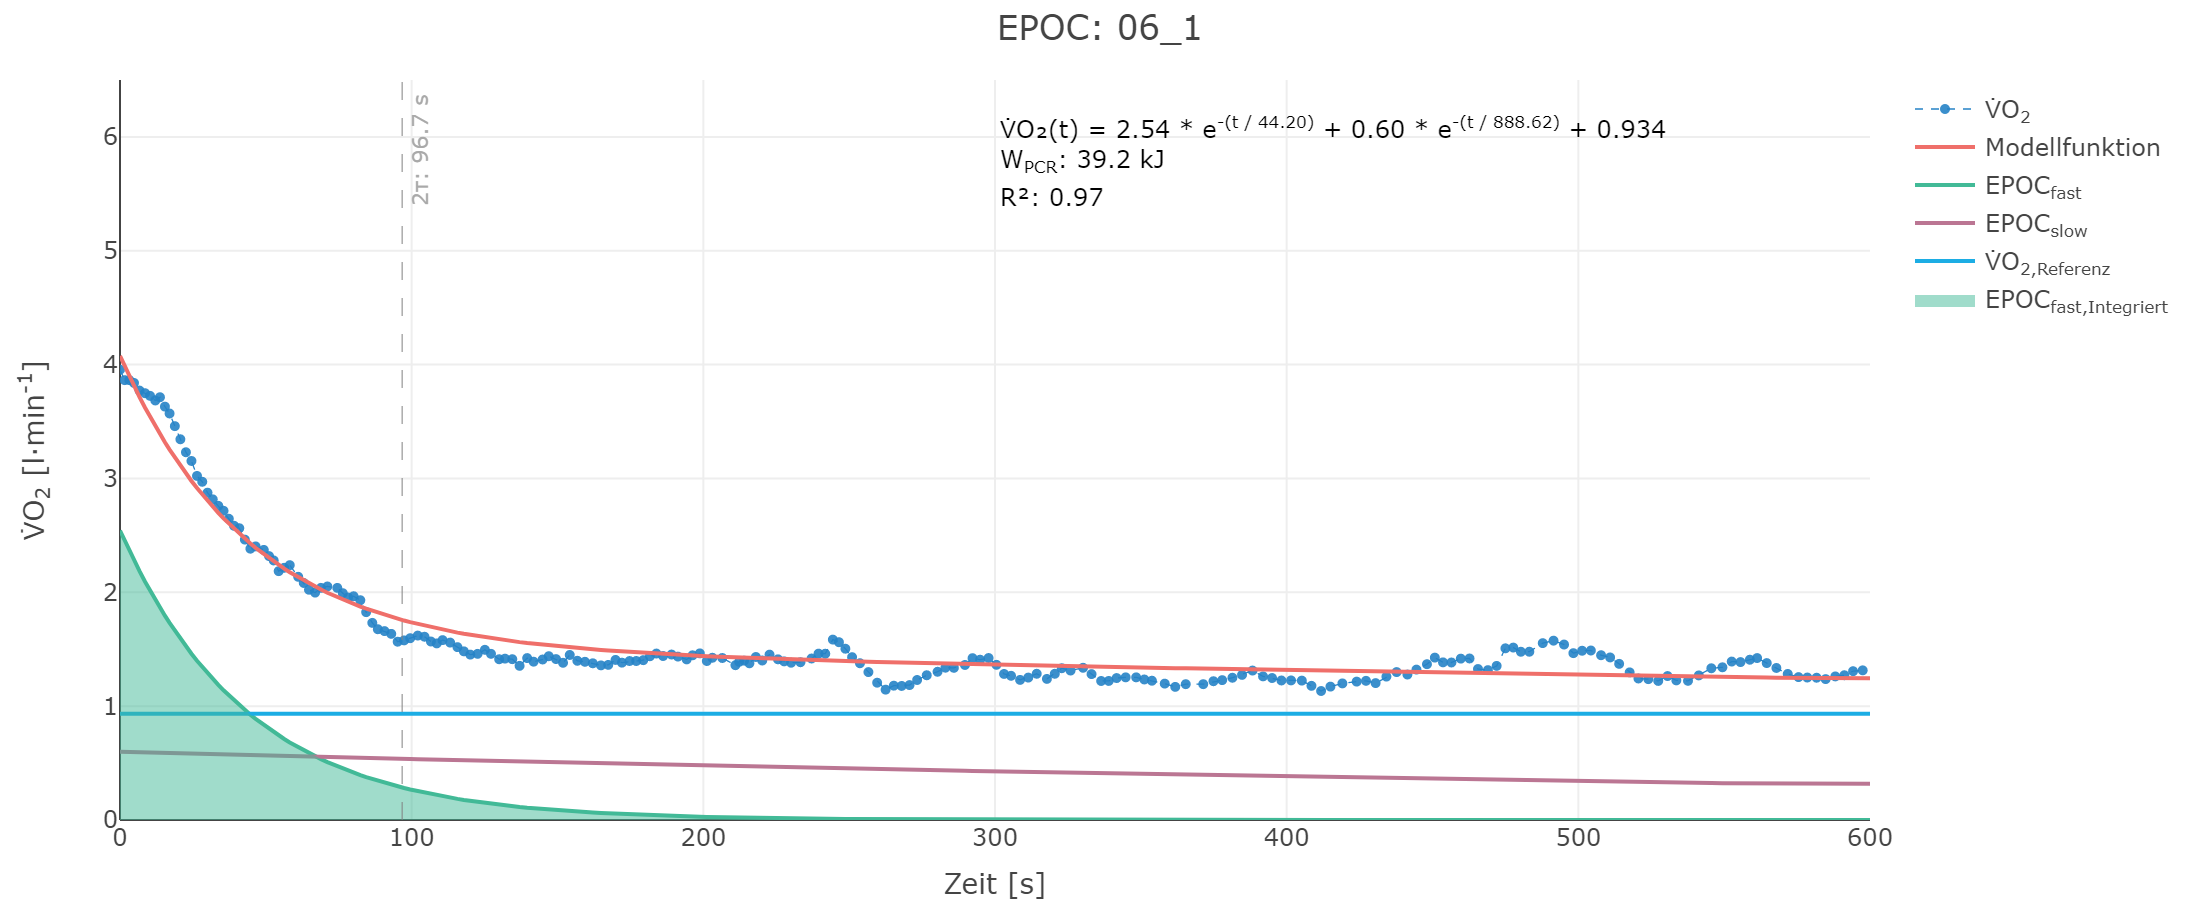
\includegraphics[width=11.45833in,height=4.6875in]{images/06_1.png}

\subsubsection{Test 2}

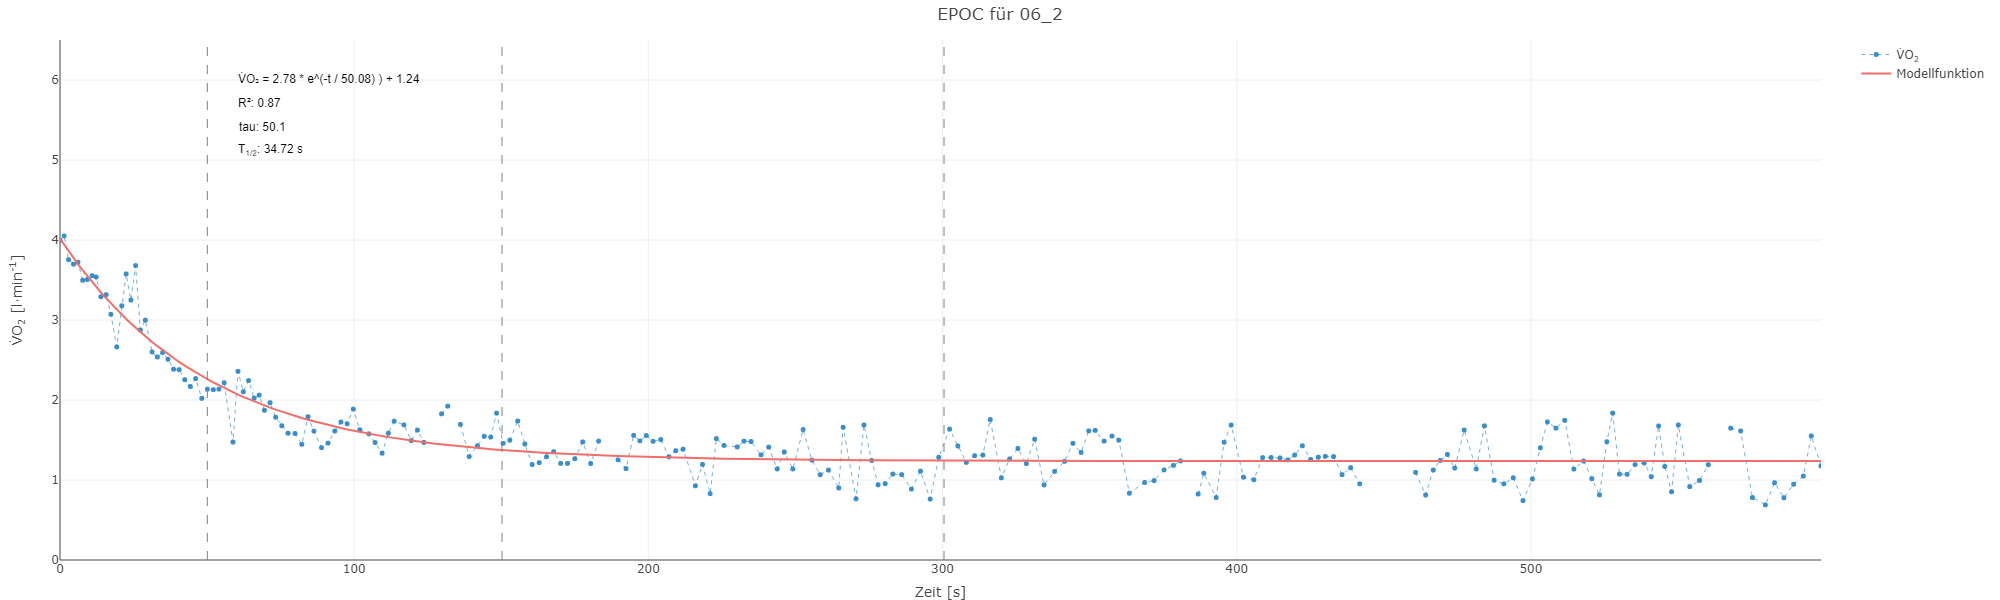
\includegraphics[width=11.45833in,height=4.6875in]{images/06_2_tau.png}
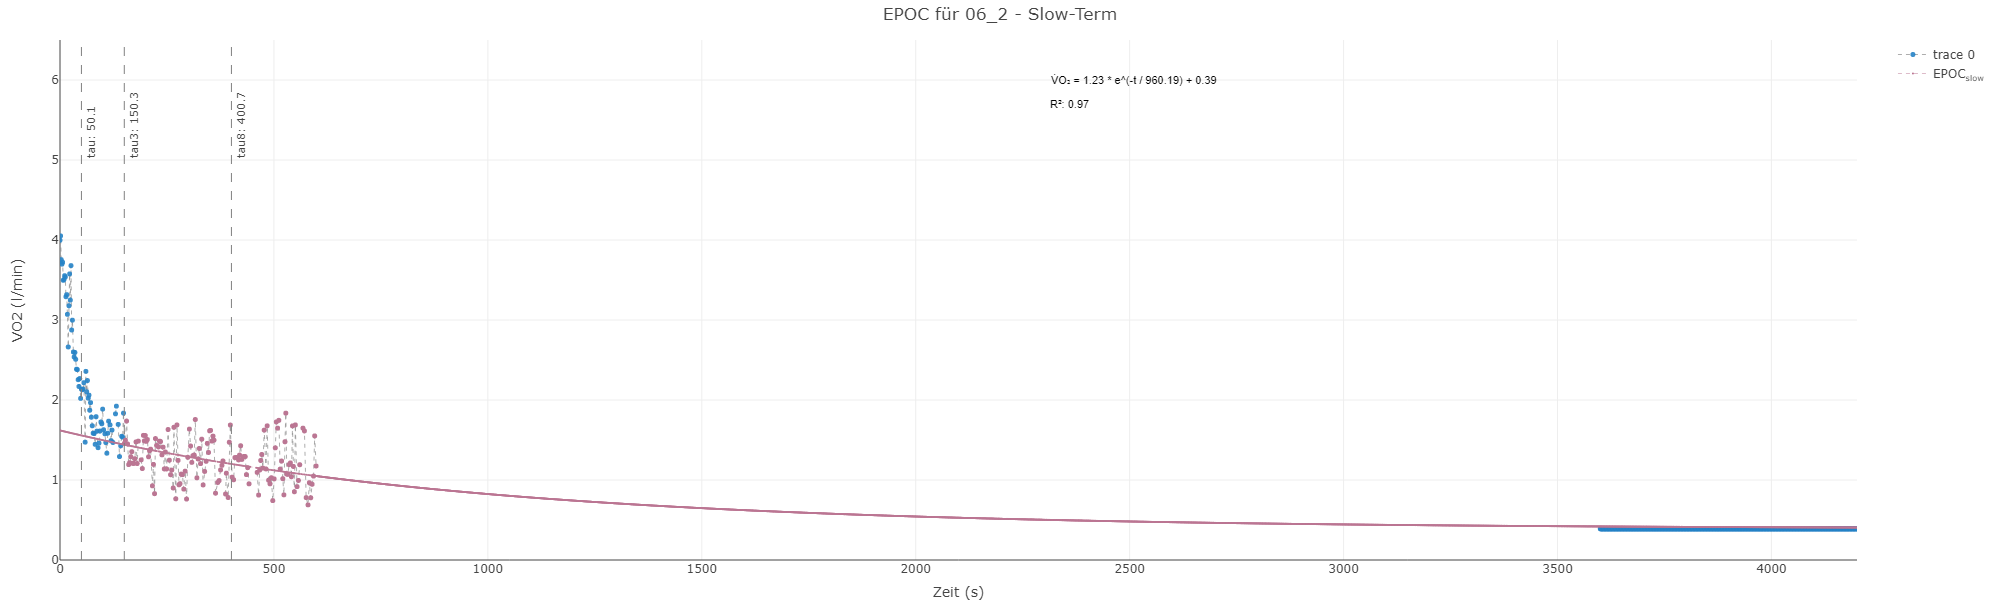
\includegraphics[width=11.45833in,height=4.6875in]{images/06_2_slow.png}
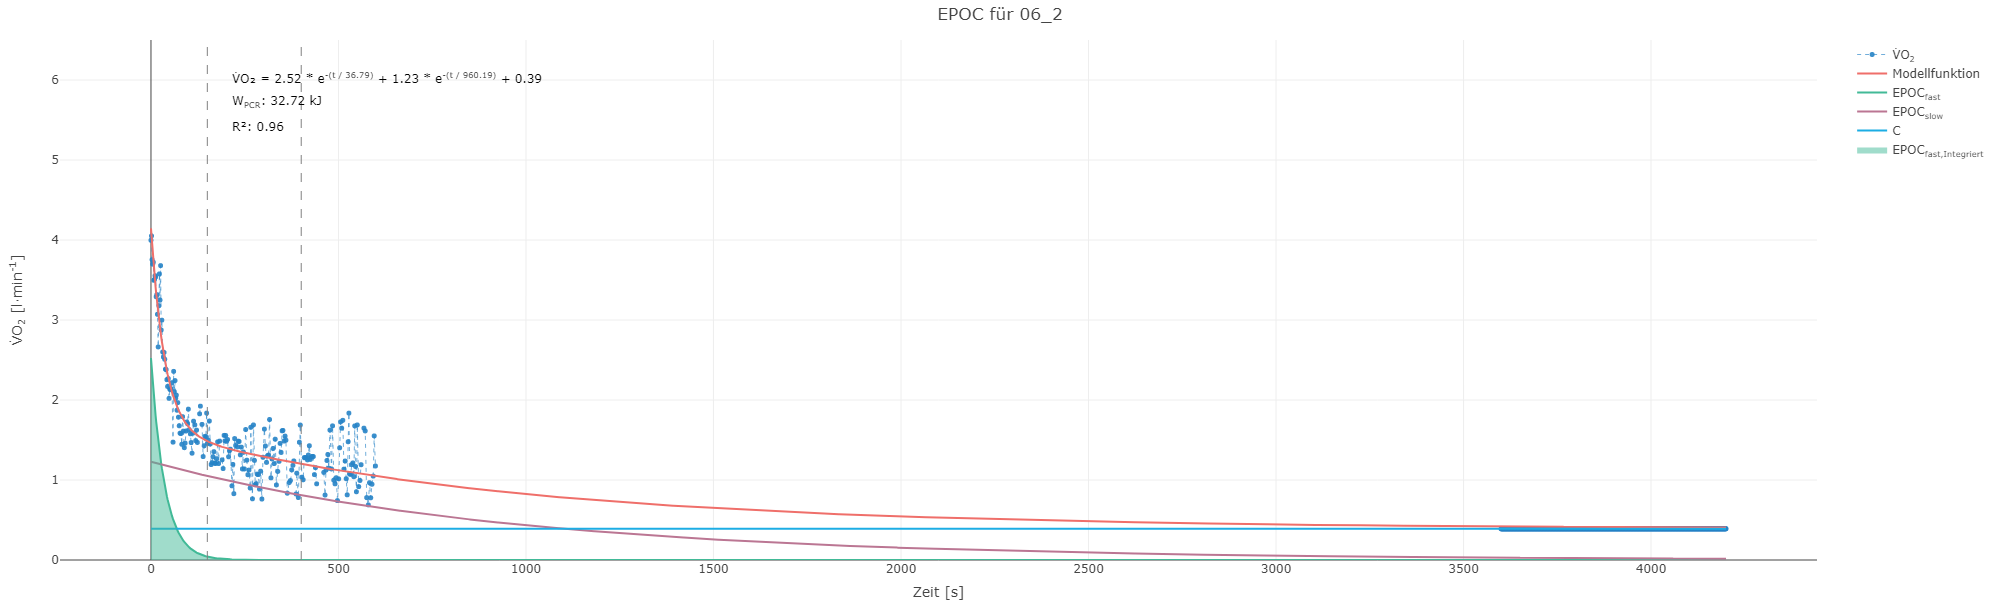
\includegraphics[width=11.45833in,height=4.6875in]{images/06_2.png}

\subsubsection{Test 3}

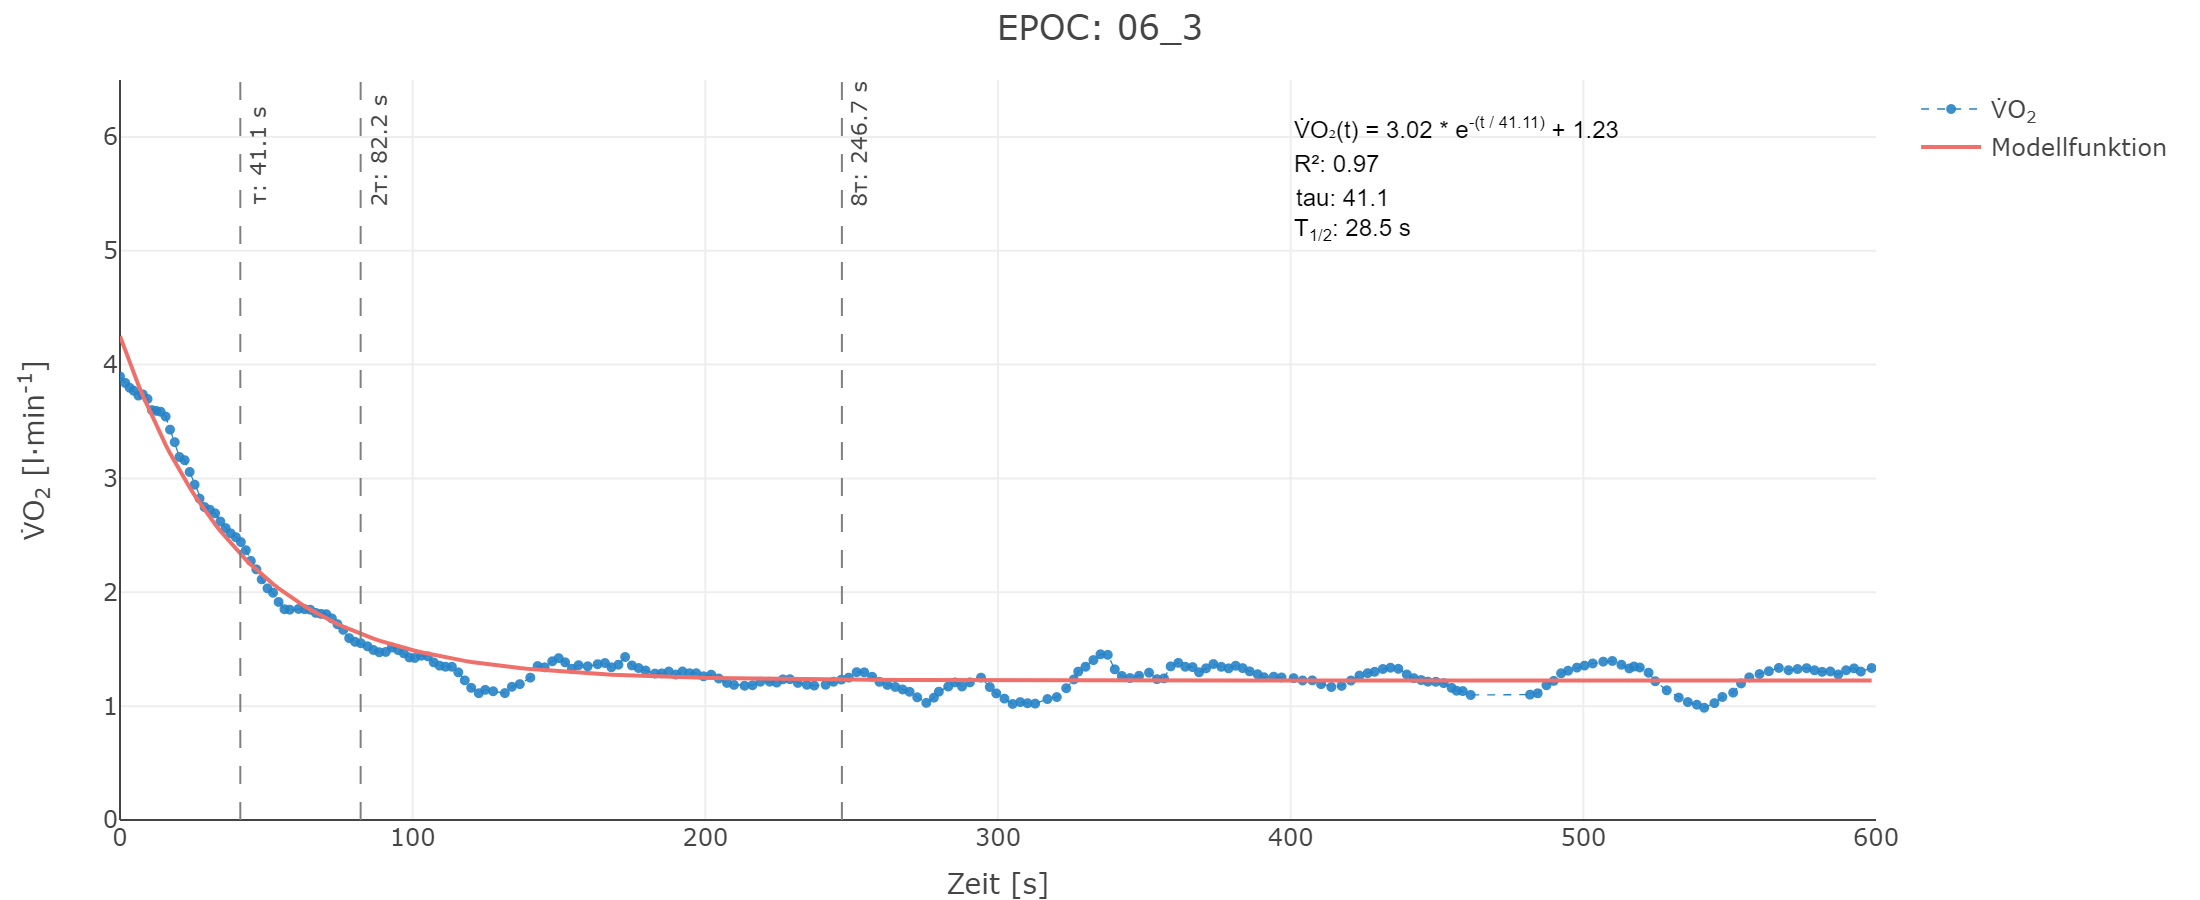
\includegraphics[width=11.45833in,height=4.6875in]{images/06_3_tau.png}
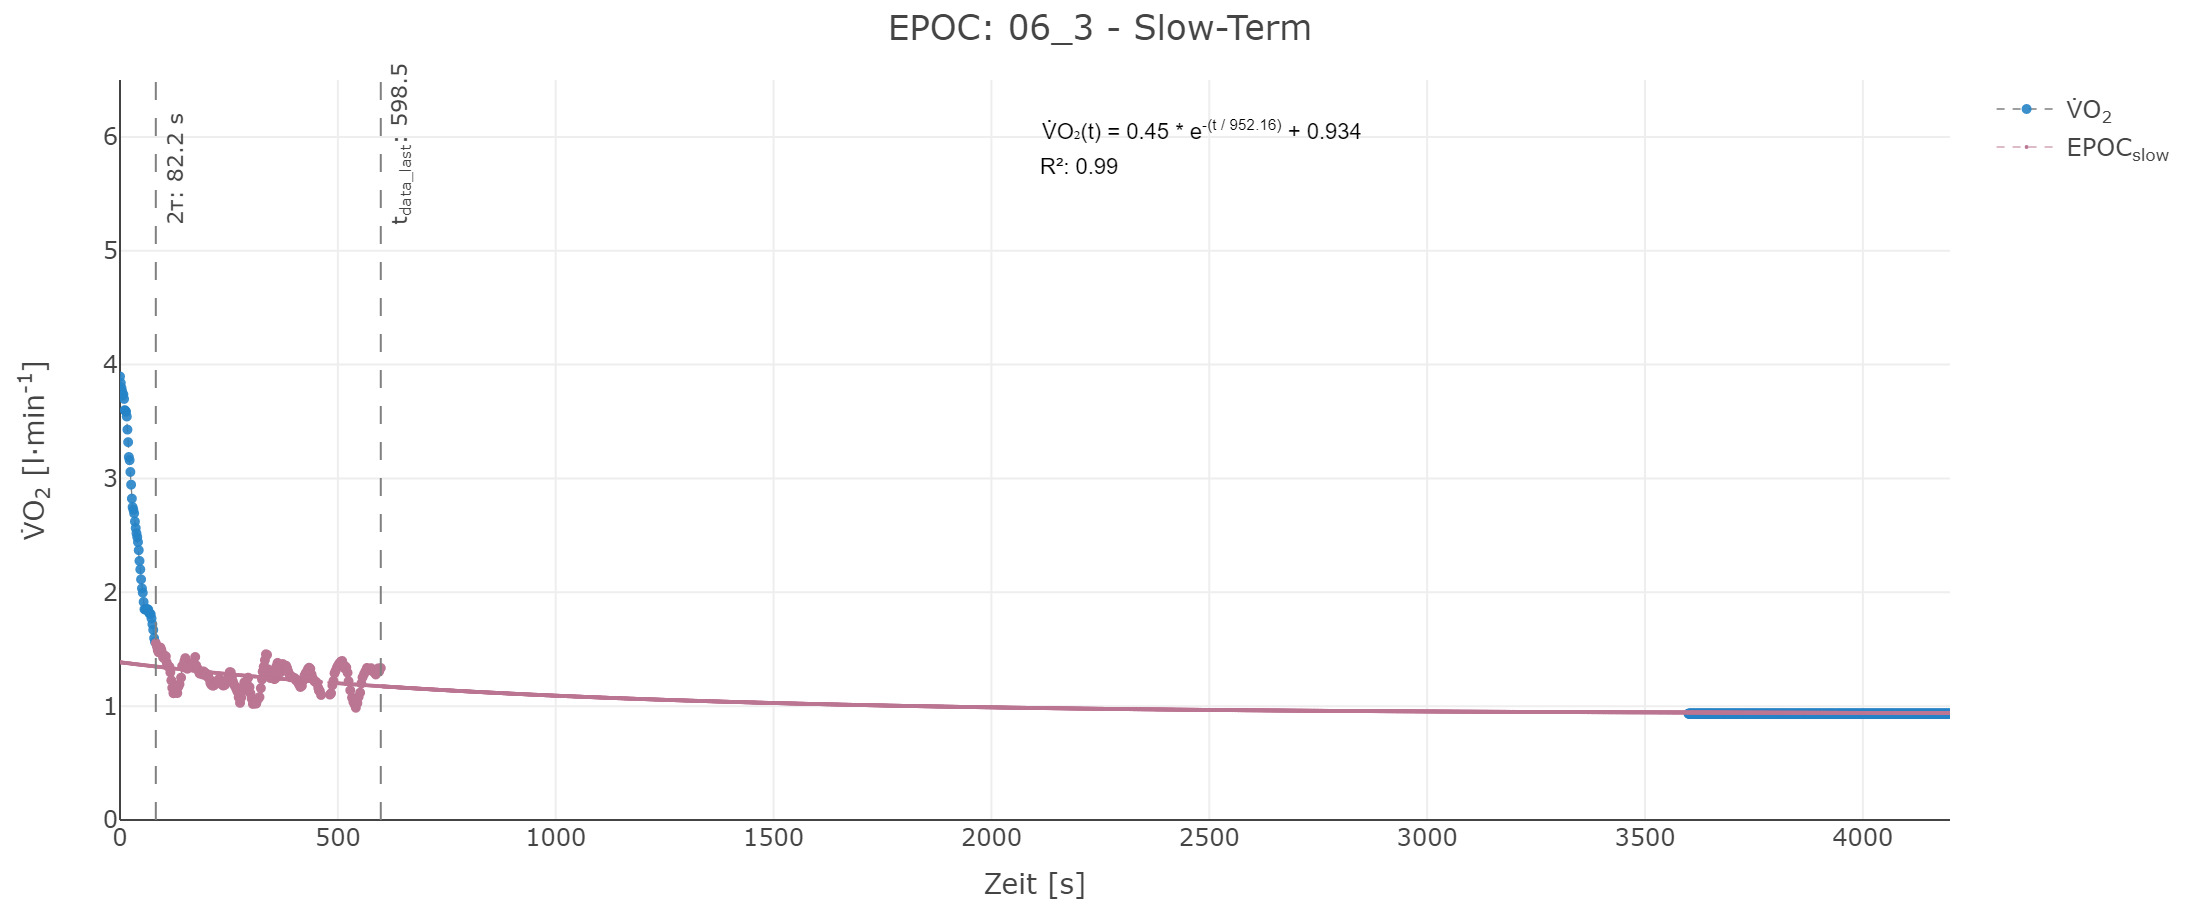
\includegraphics[width=11.45833in,height=4.6875in]{images/06_3_slow.png}
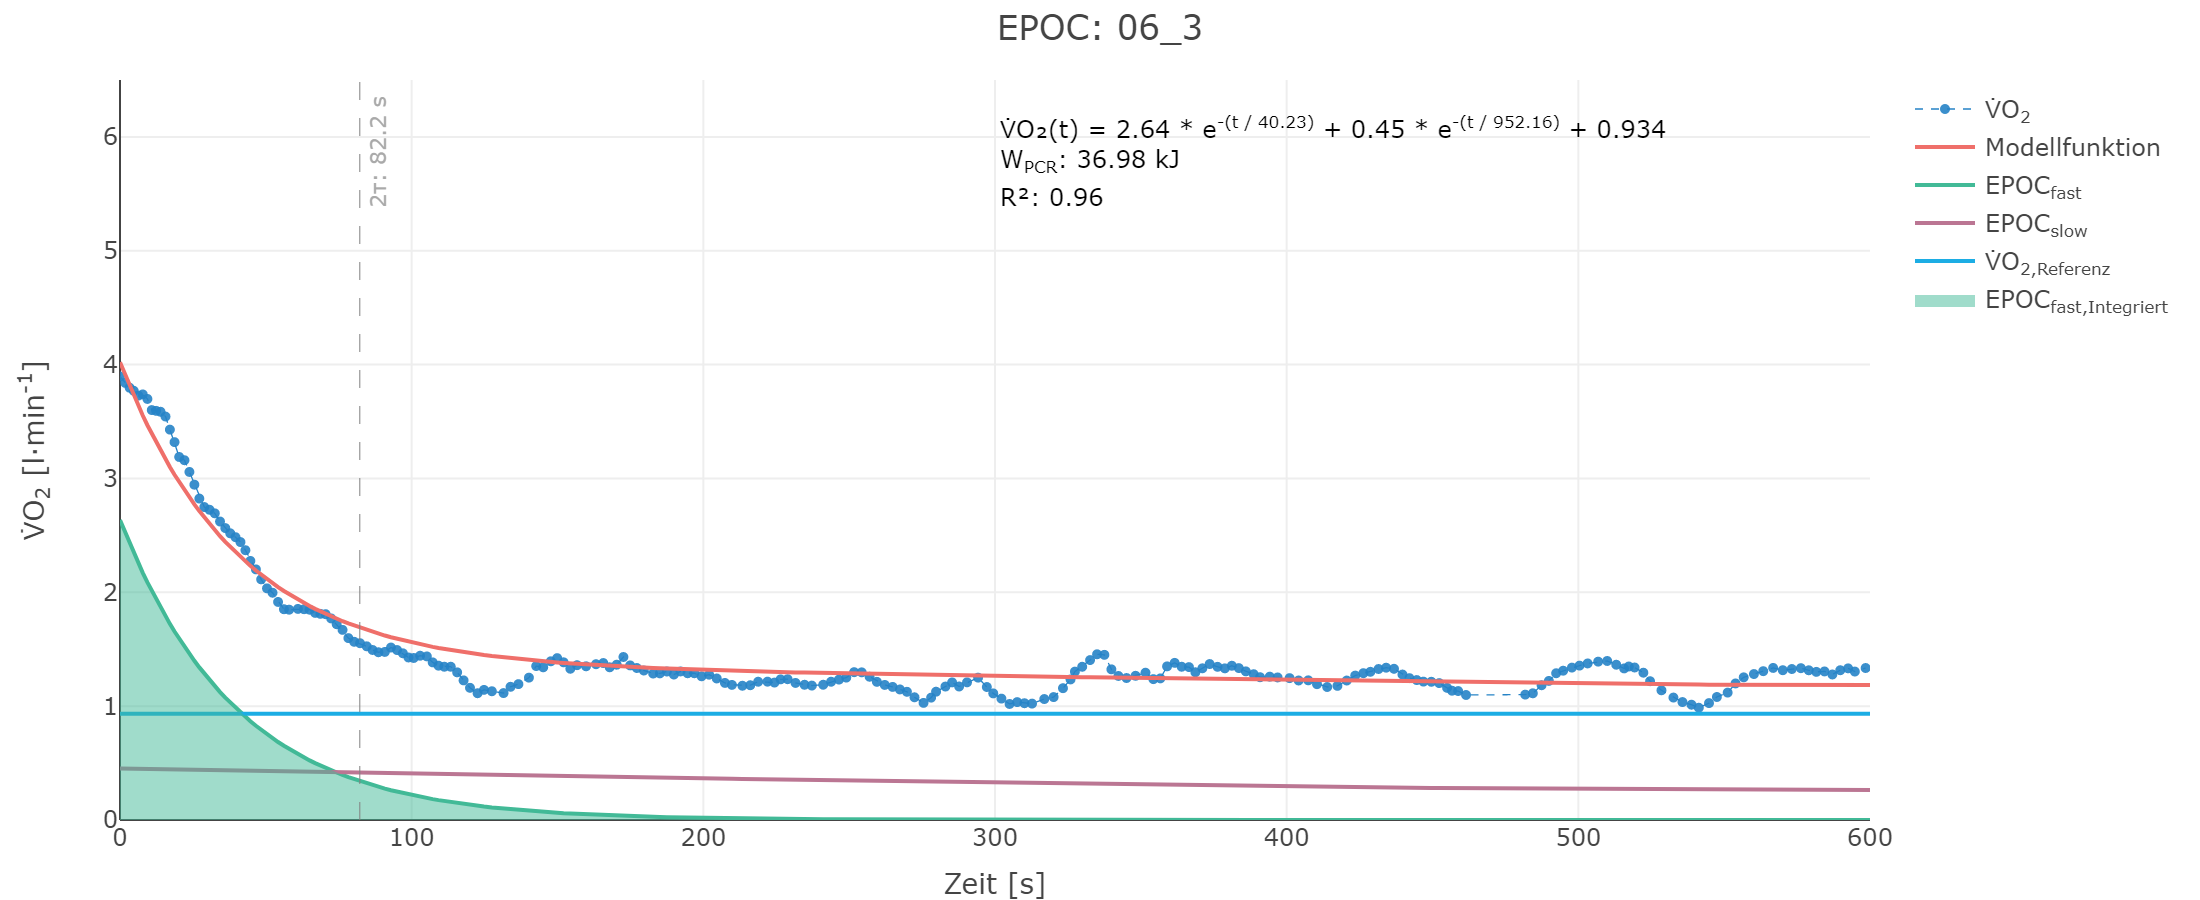
\includegraphics[width=11.45833in,height=4.6875in]{images/06_3.png}

\subsubsection{Test 4}

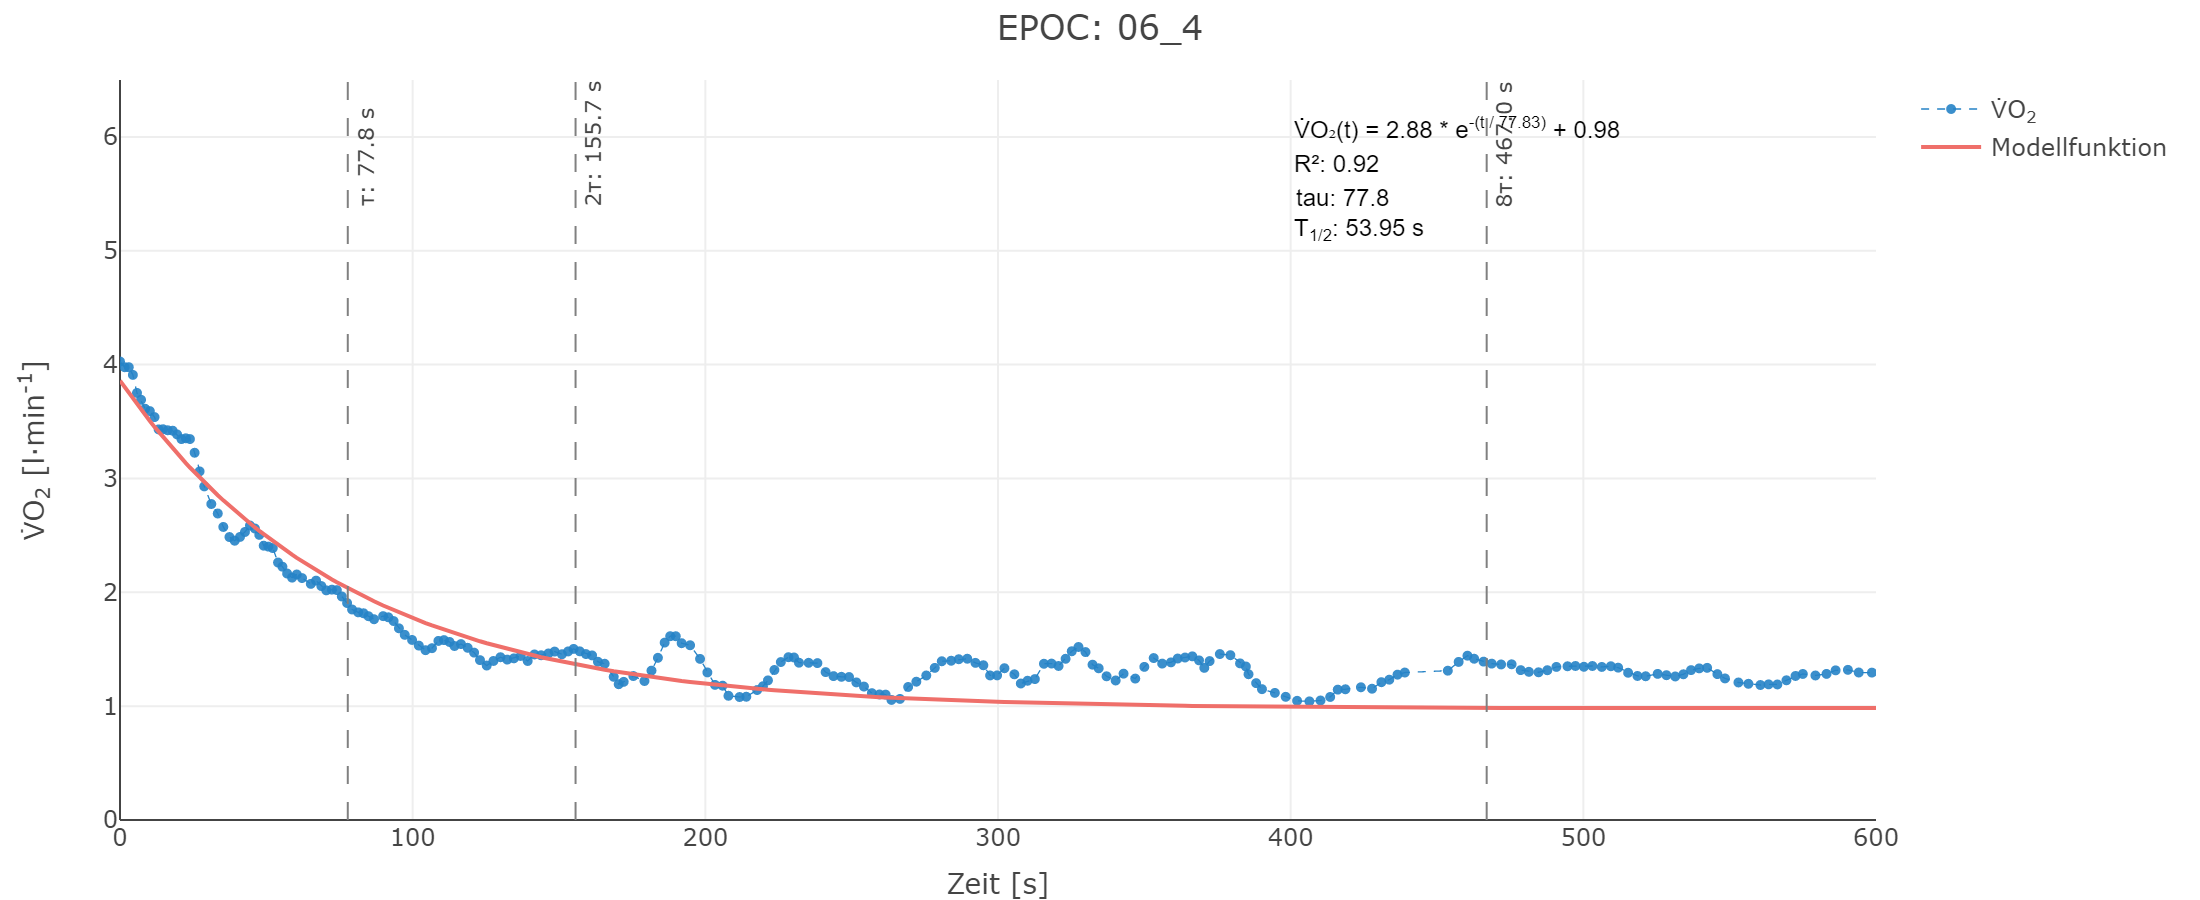
\includegraphics[width=11.45833in,height=4.6875in]{images/06_4_tau.png}
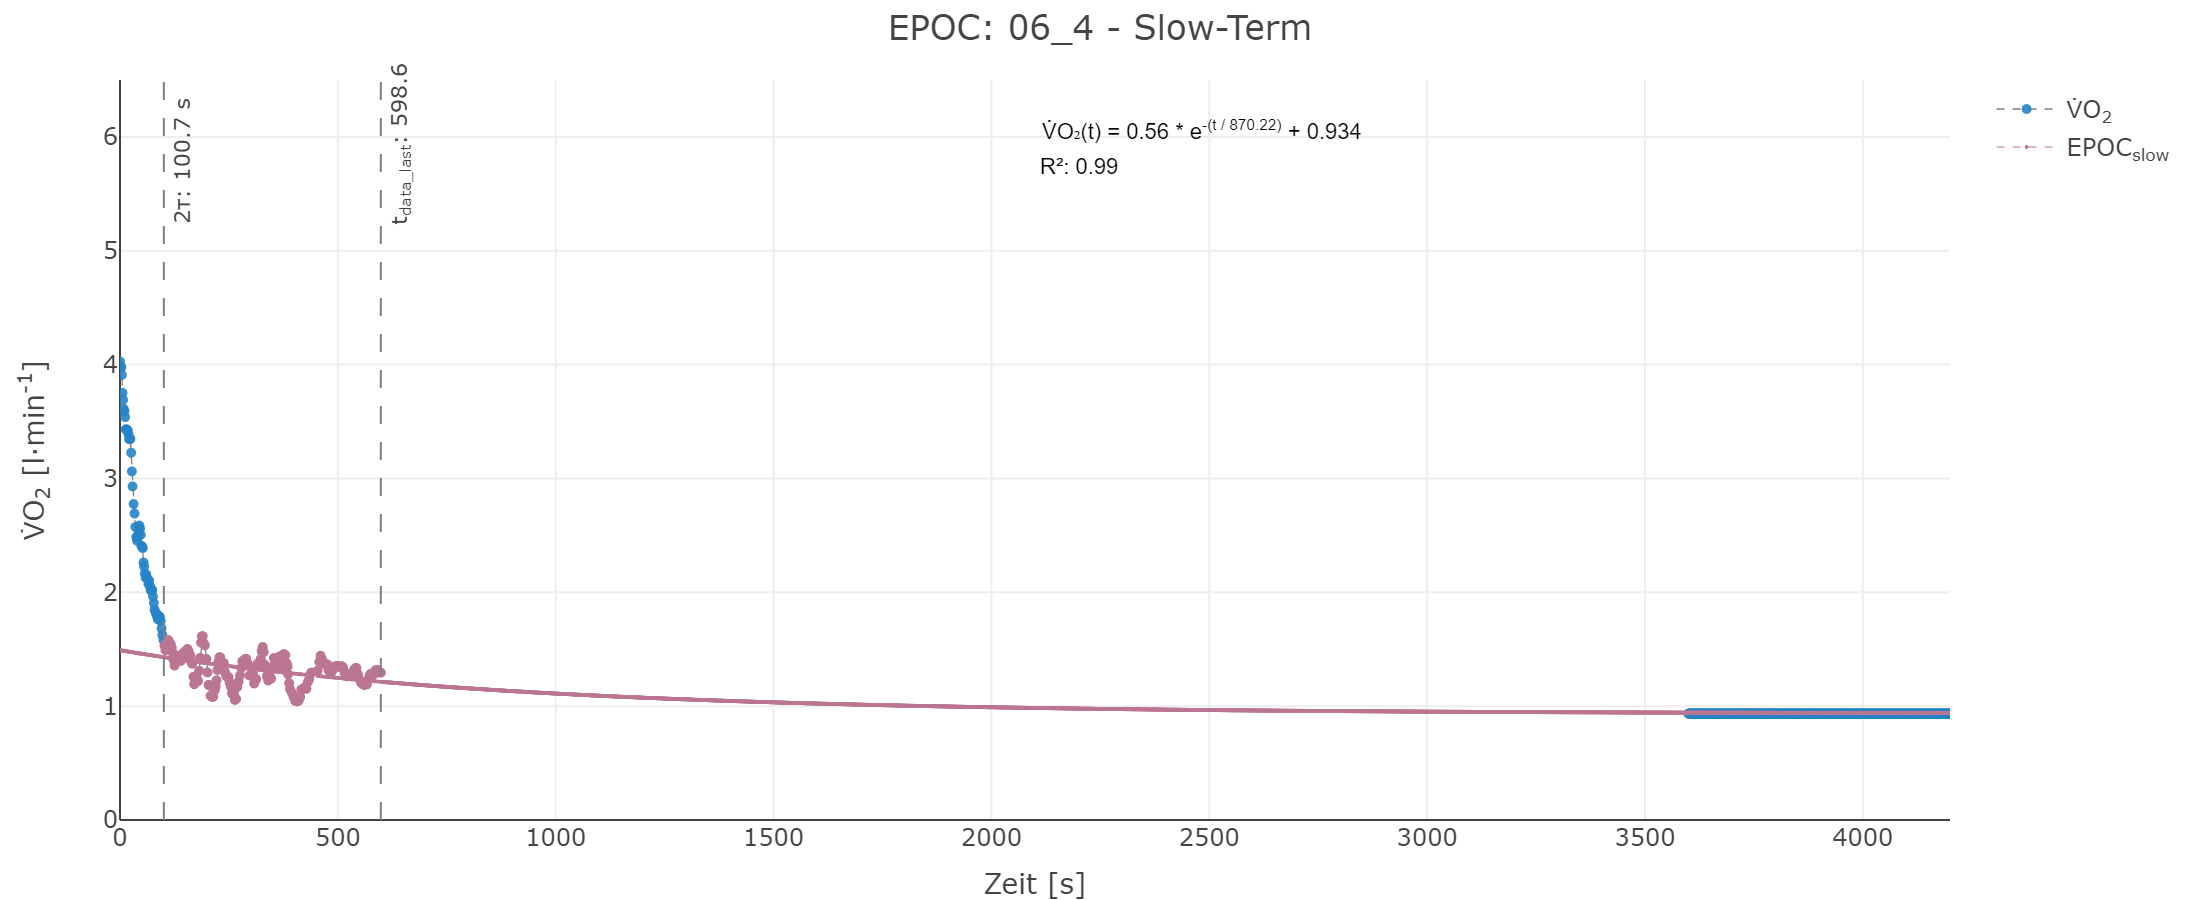
\includegraphics[width=11.45833in,height=4.6875in]{images/06_4_slow.png}
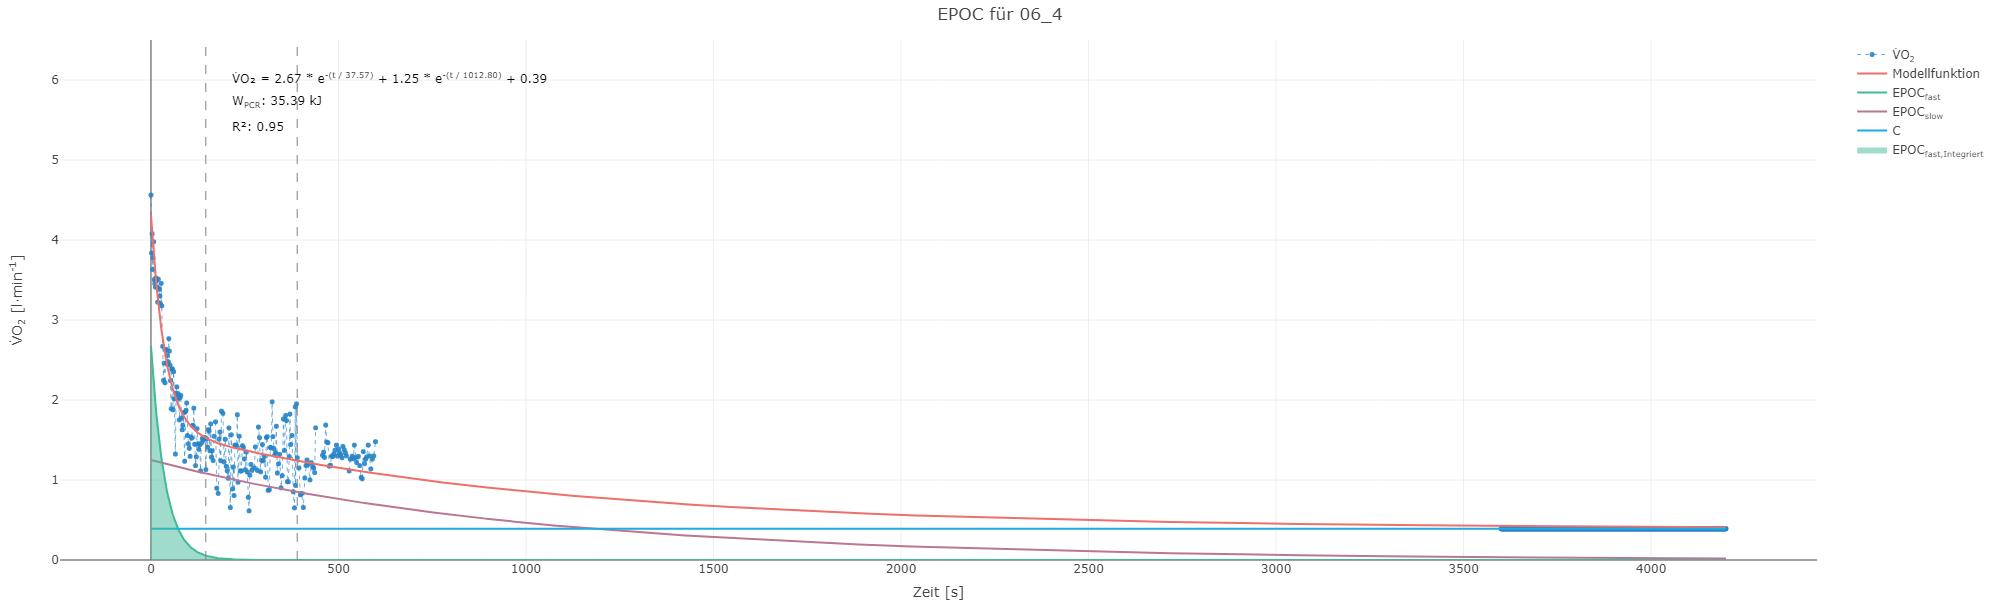
\includegraphics[width=11.45833in,height=4.6875in]{images/06_4.png}

\subsubsection{Test 5}

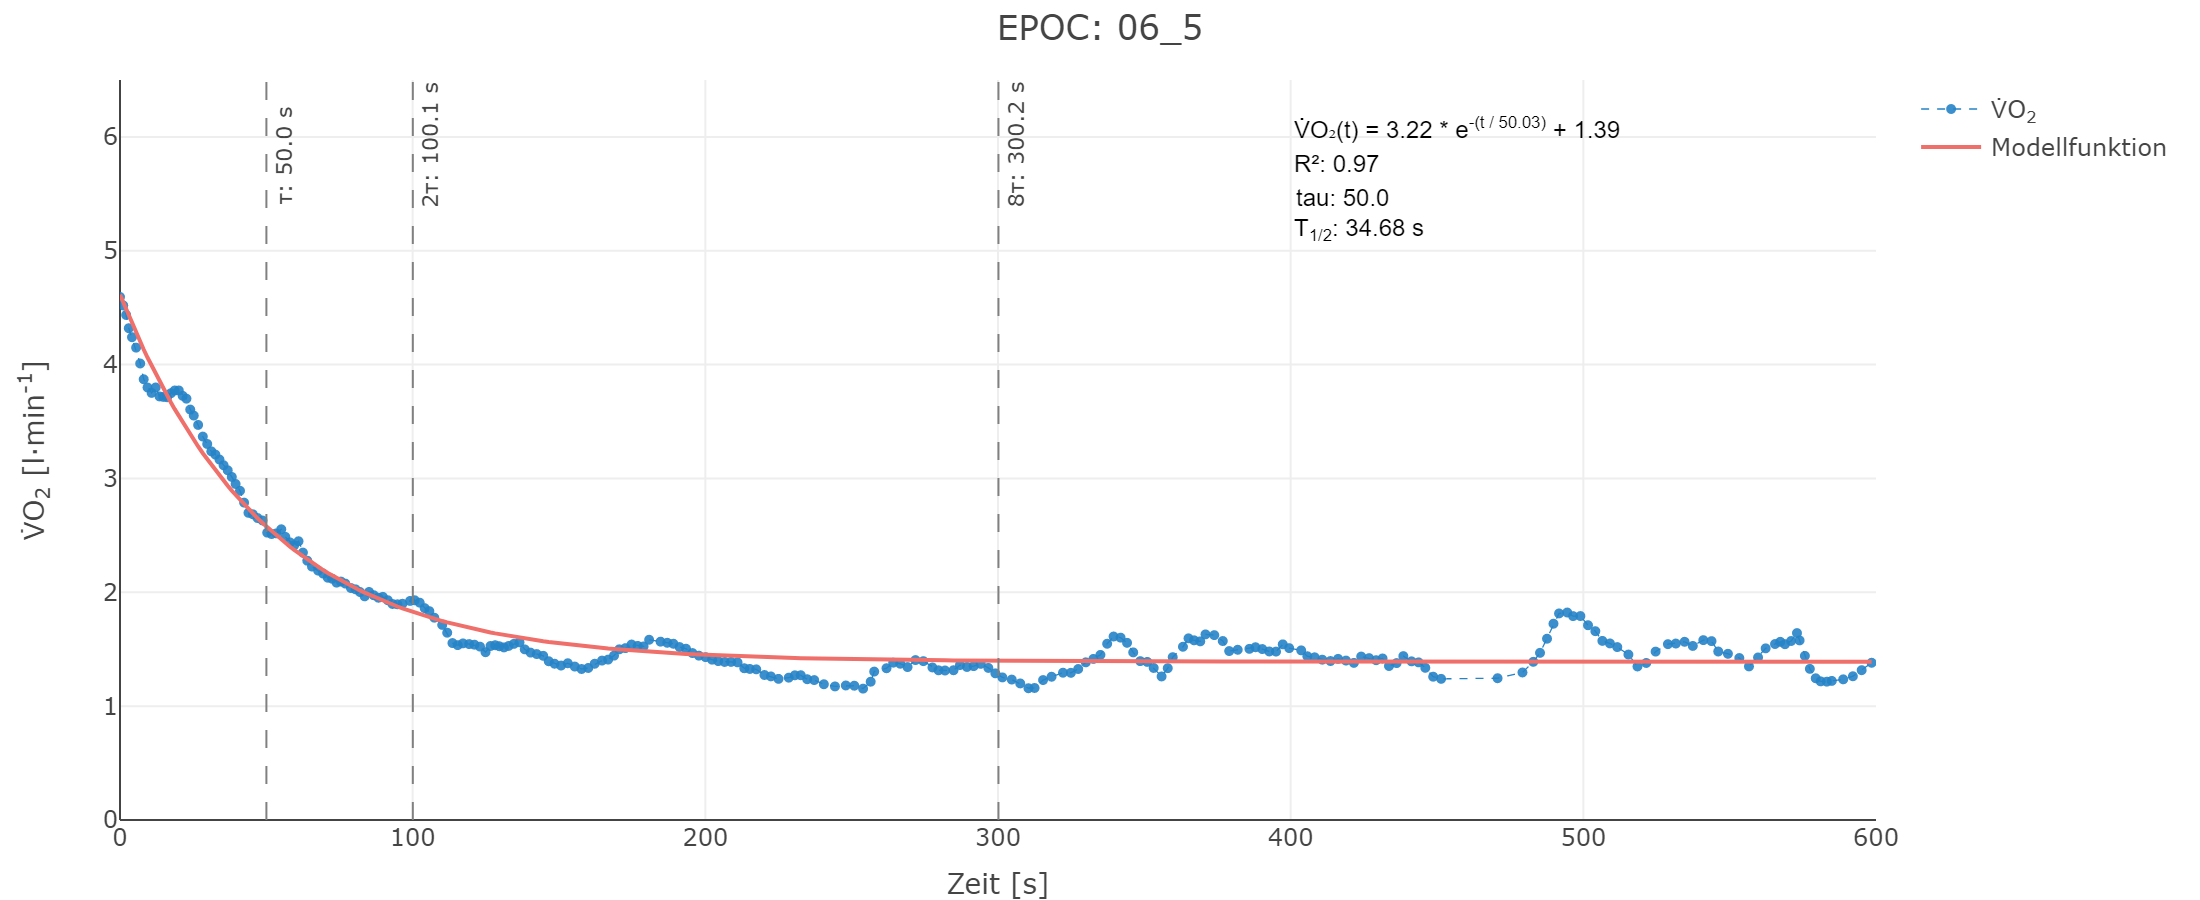
\includegraphics[width=11.45833in,height=4.6875in]{images/06_5_tau.png}
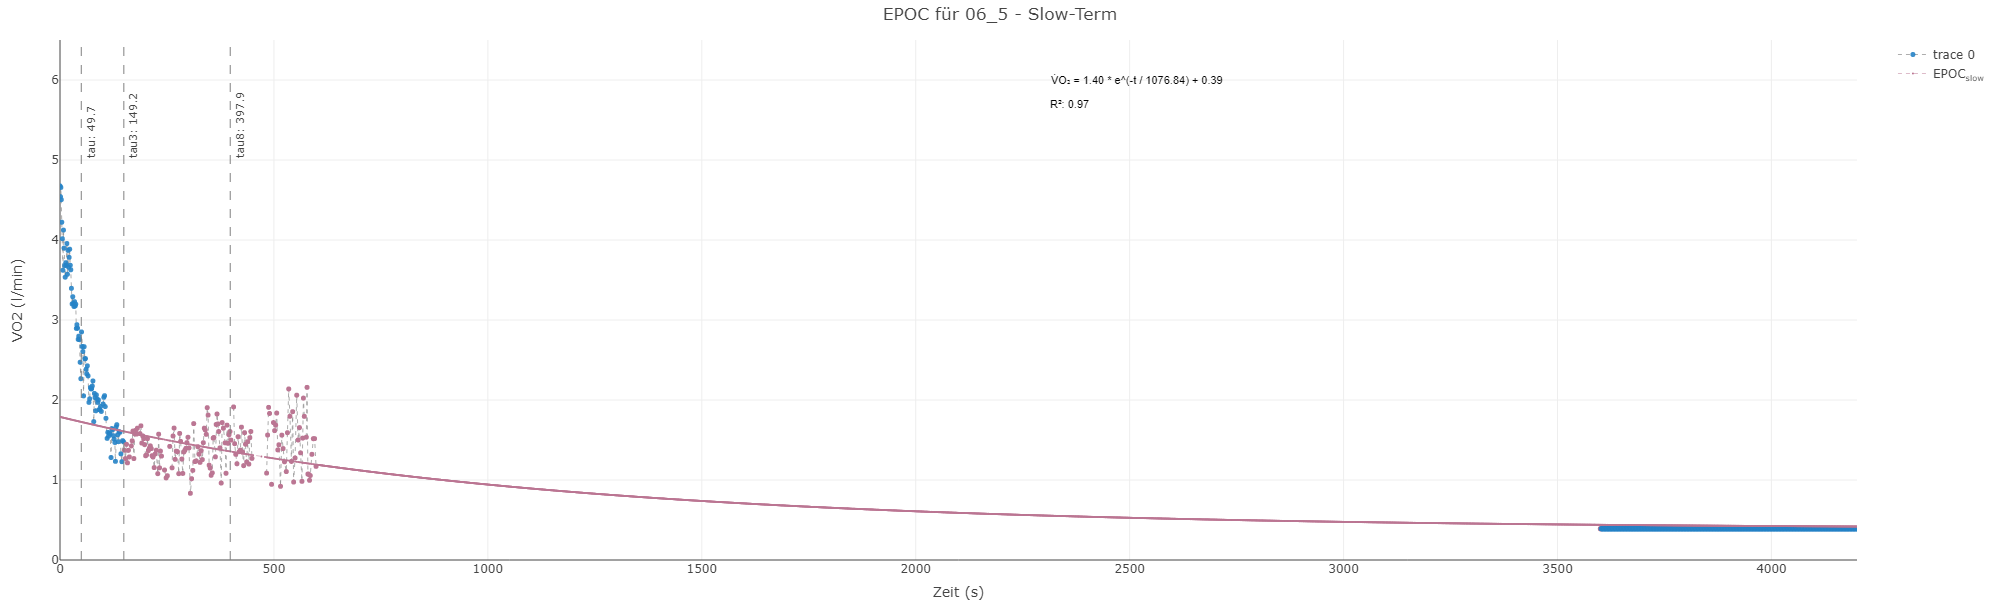
\includegraphics[width=11.45833in,height=4.6875in]{images/06_5_slow.png}
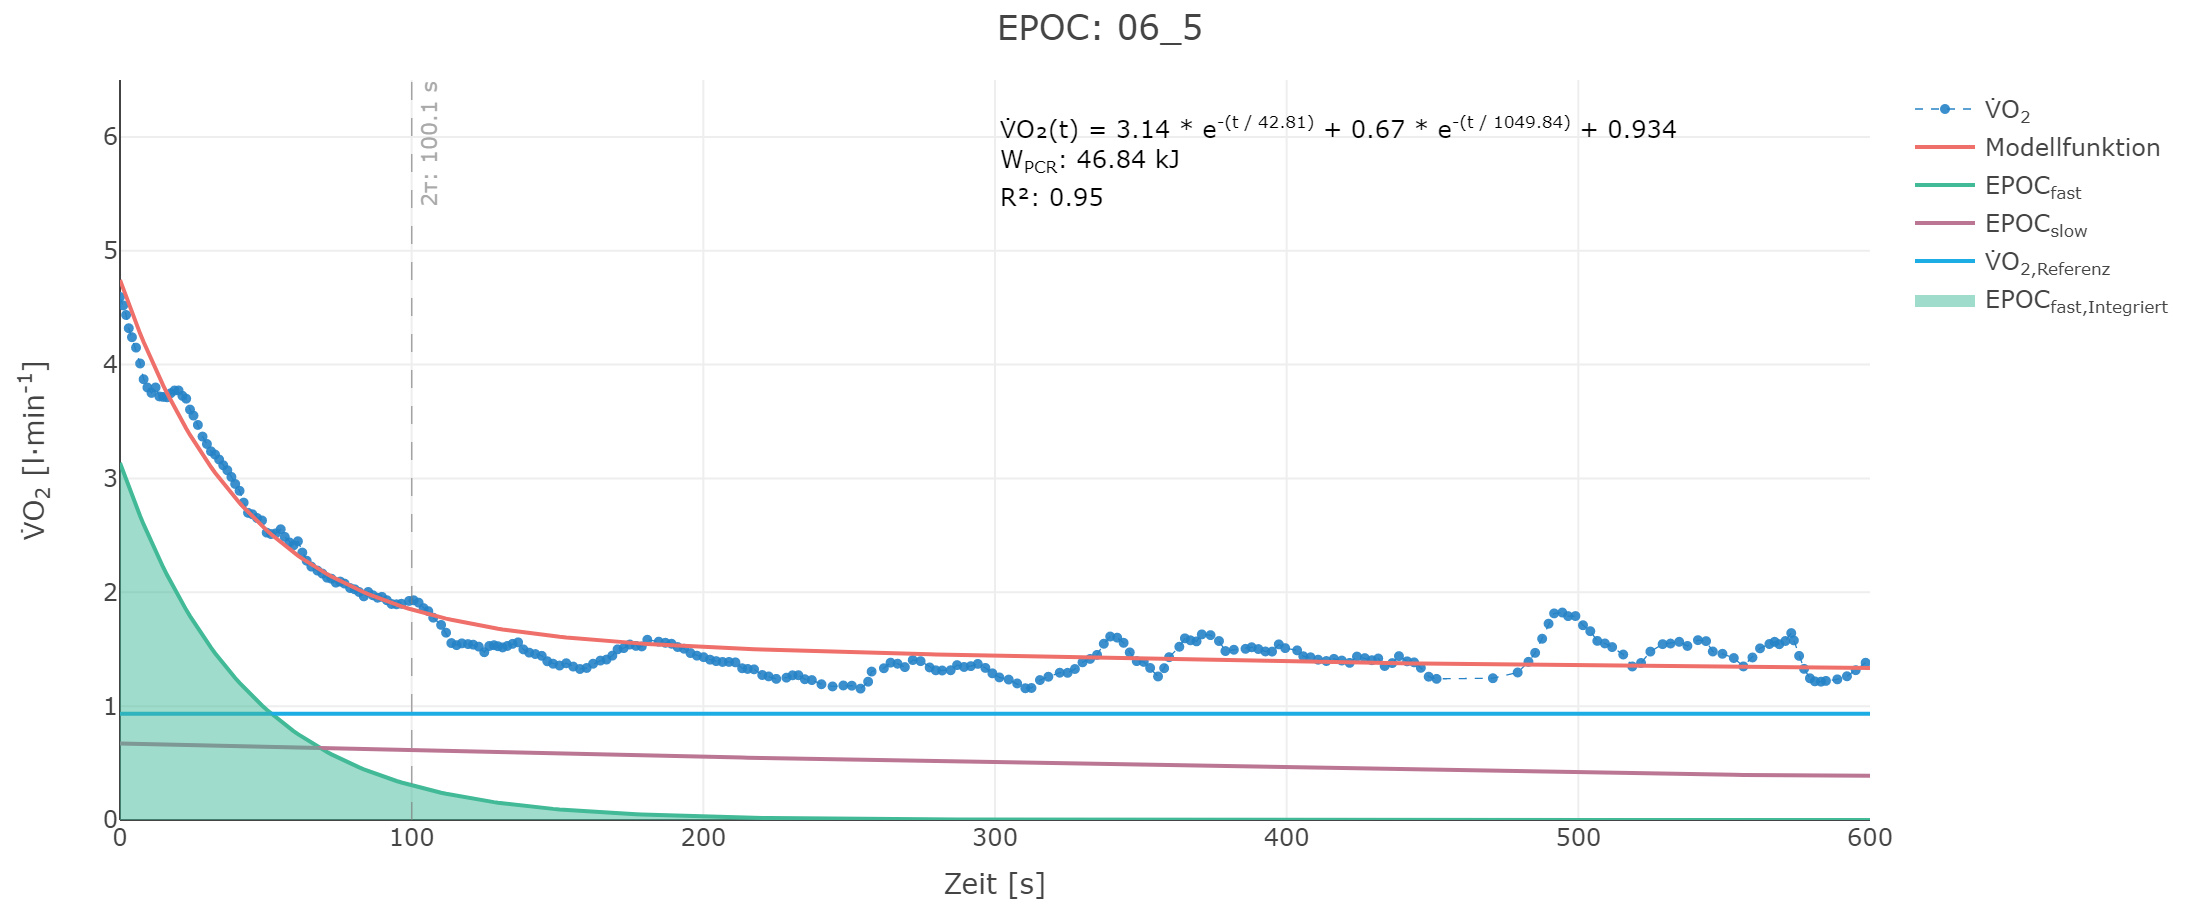
\includegraphics[width=11.45833in,height=4.6875in]{images/06_5.png}

\subsubsection{Test 6}

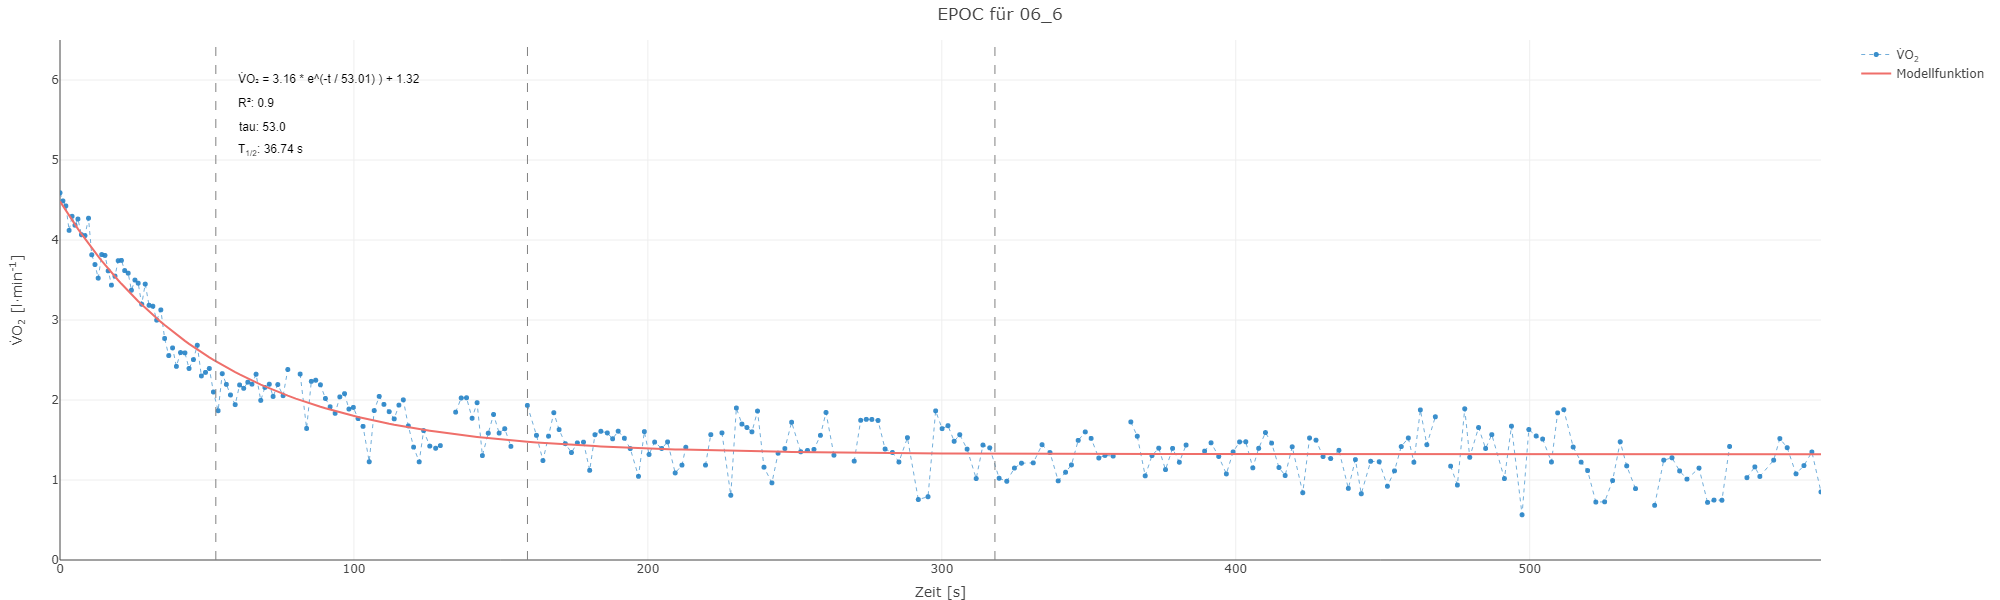
\includegraphics[width=11.45833in,height=4.6875in]{images/06_6_tau.png}
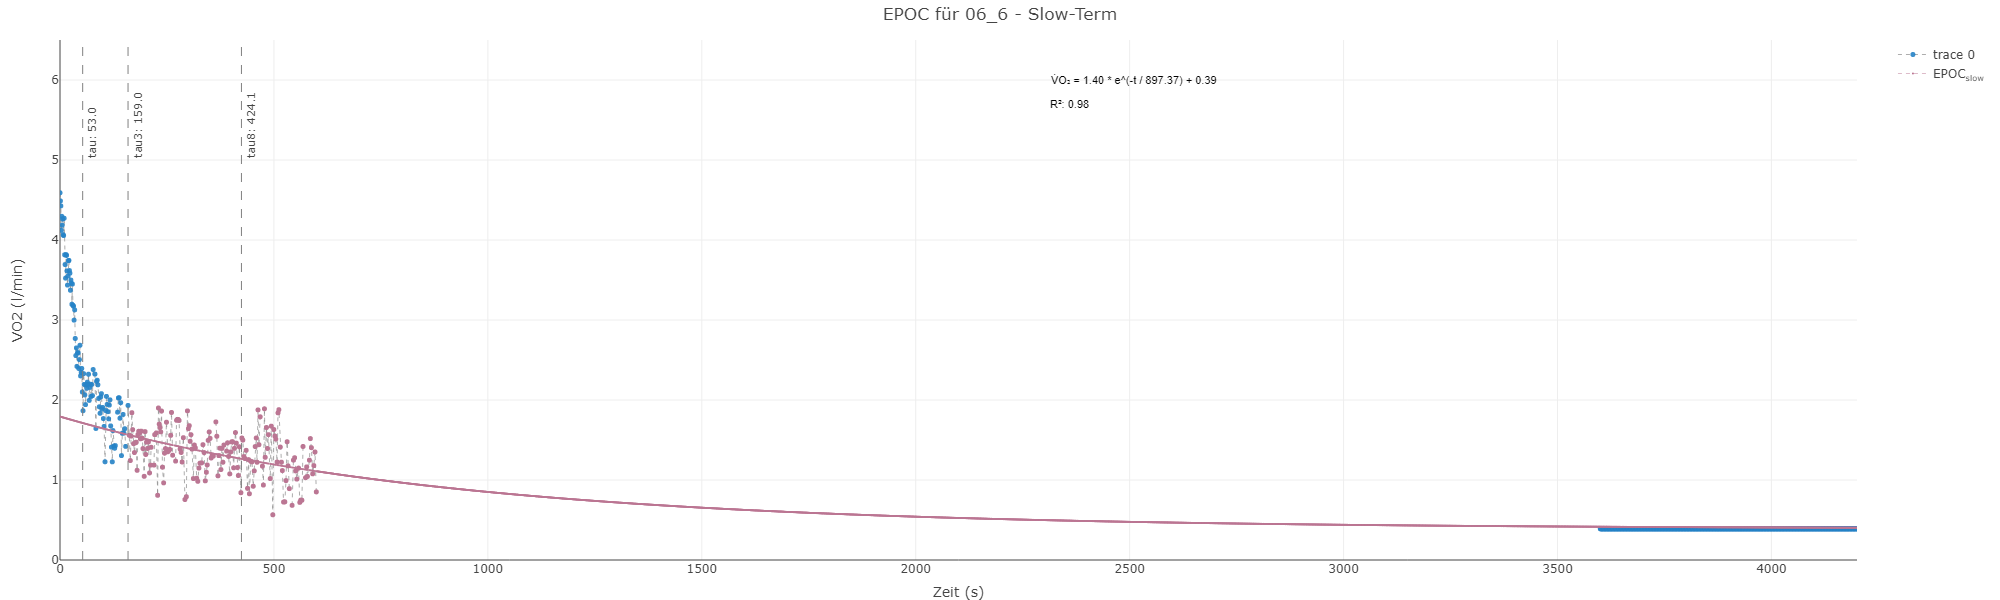
\includegraphics[width=11.45833in,height=4.6875in]{images/06_6_slow.png}
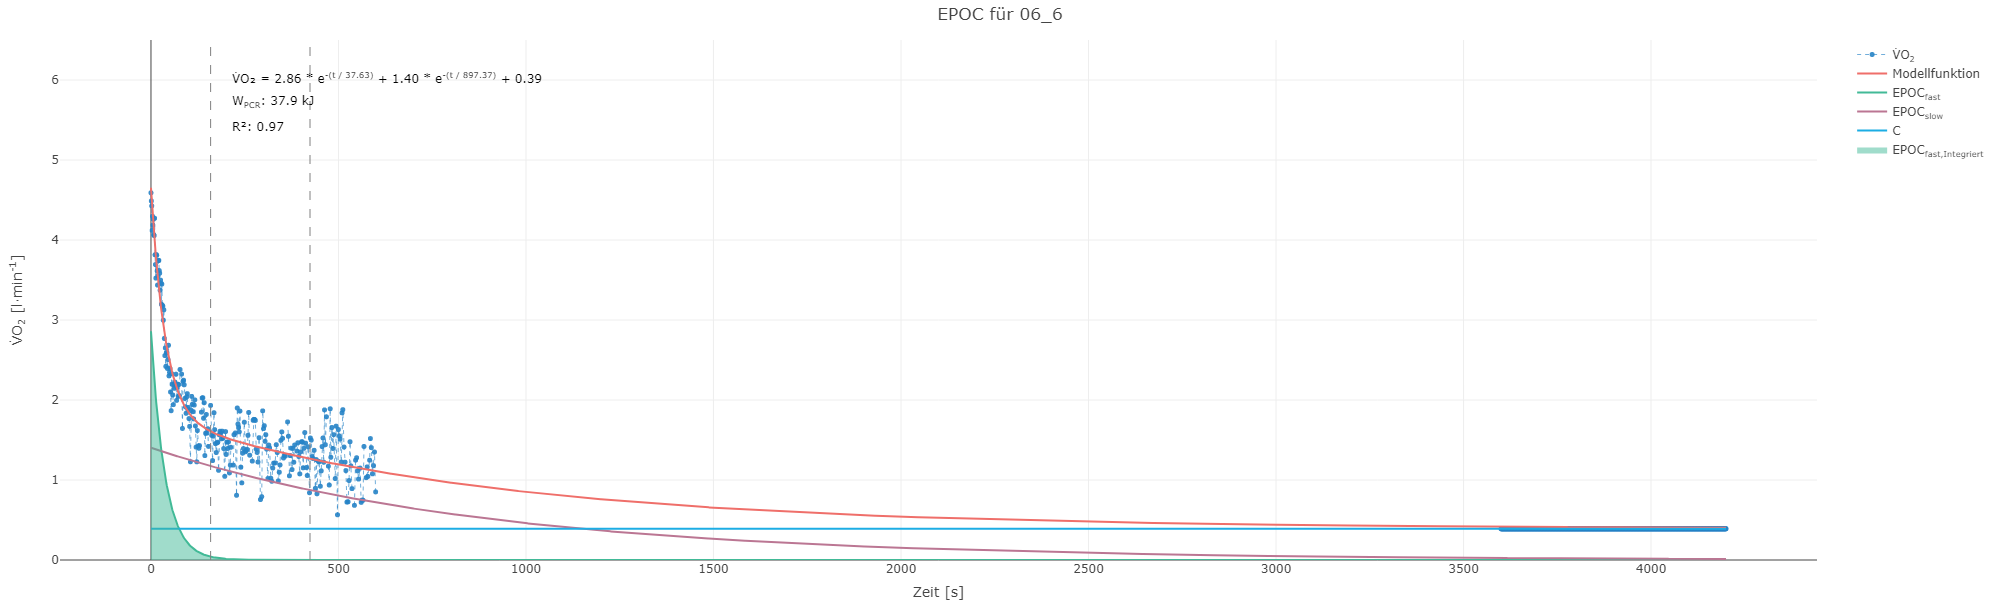
\includegraphics[width=11.45833in,height=4.6875in]{images/06_6.png}

\subsection{Proband 10}

\subsubsection{Test 1}

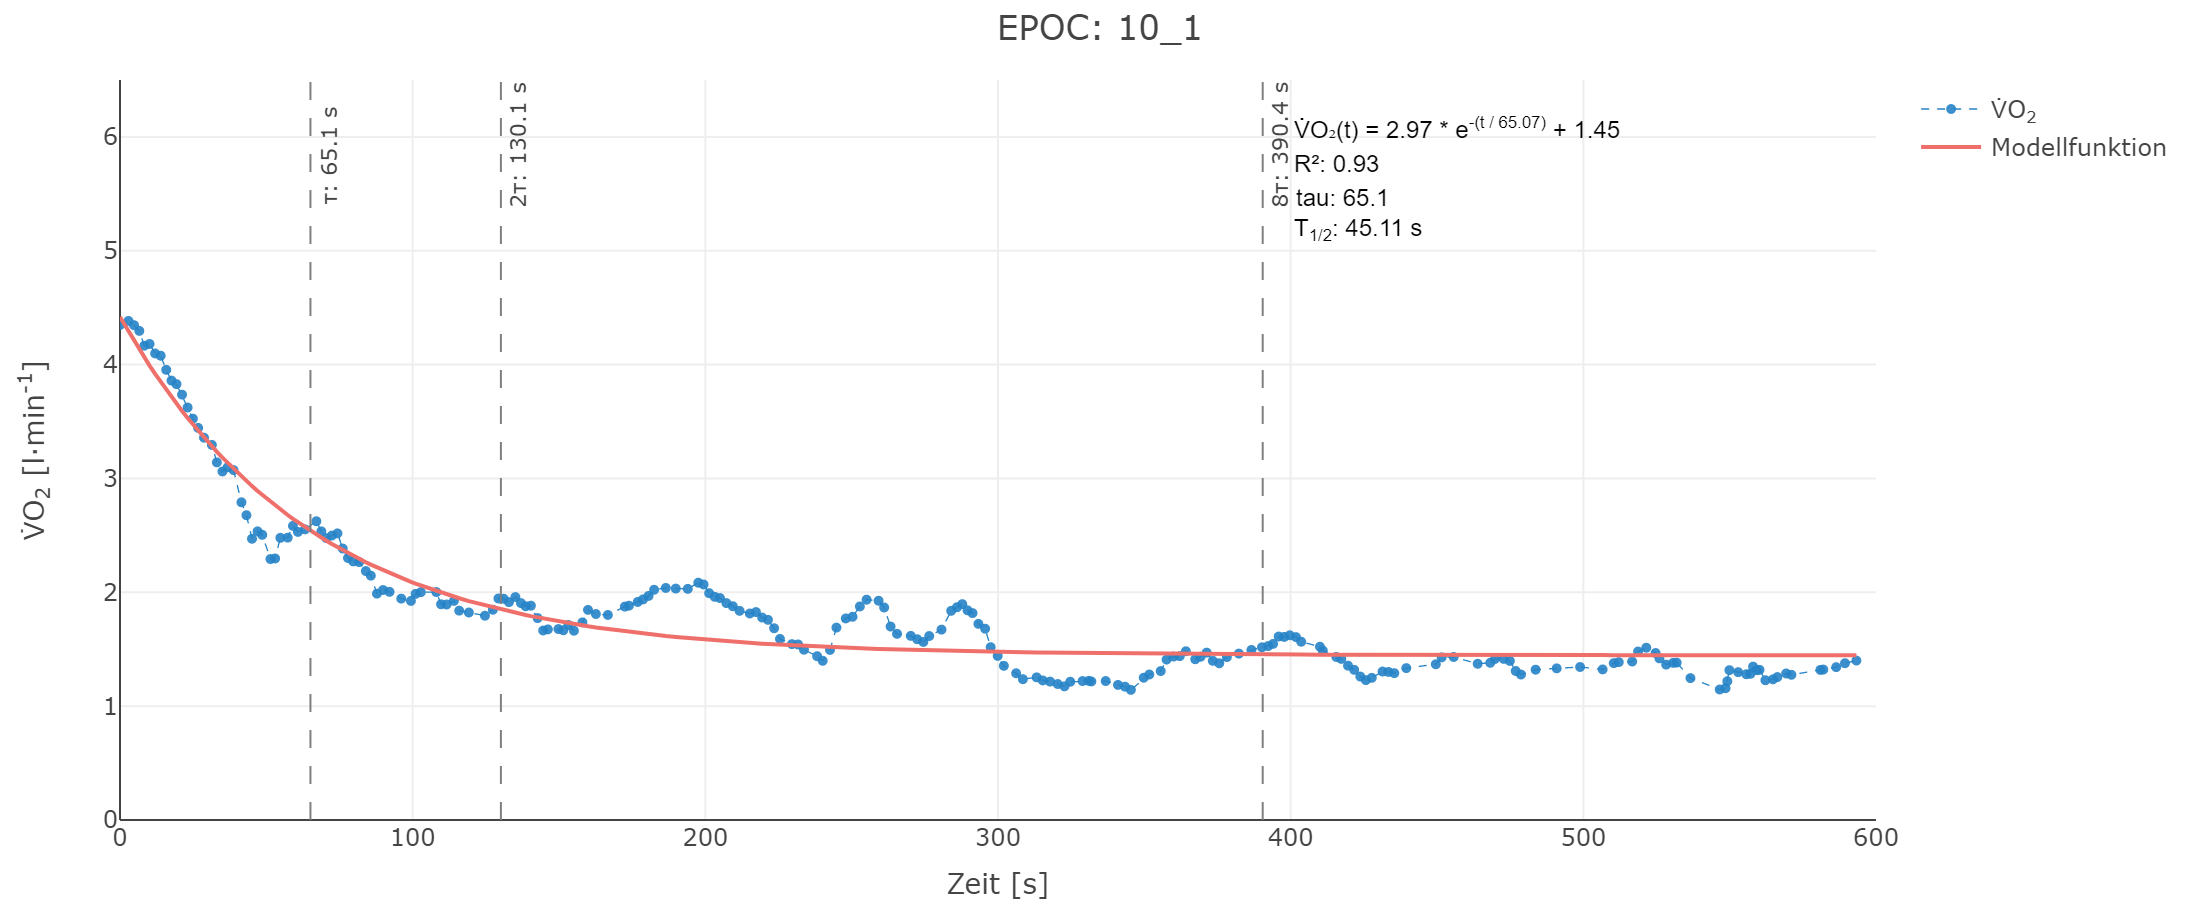
\includegraphics[width=11.45833in,height=4.6875in]{images/10_1_tau.png}
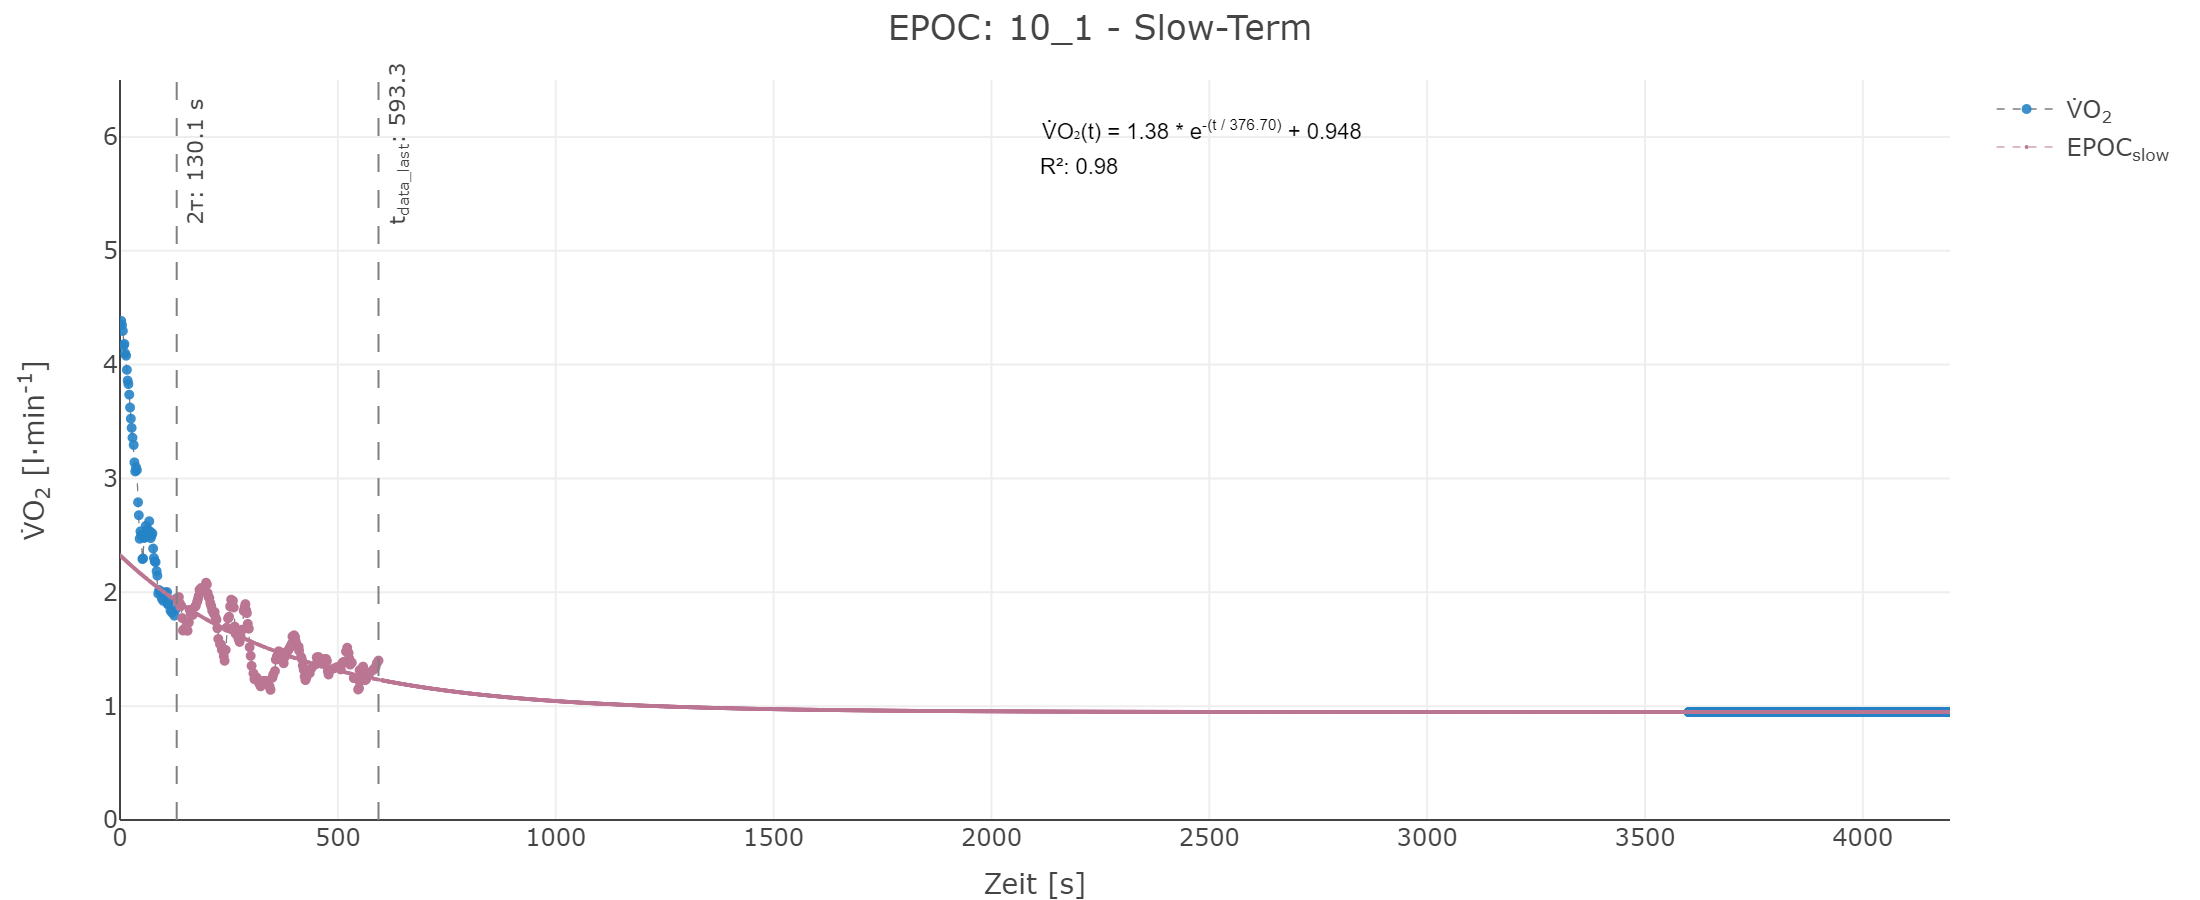
\includegraphics[width=11.45833in,height=4.6875in]{images/10_1_slow.png}
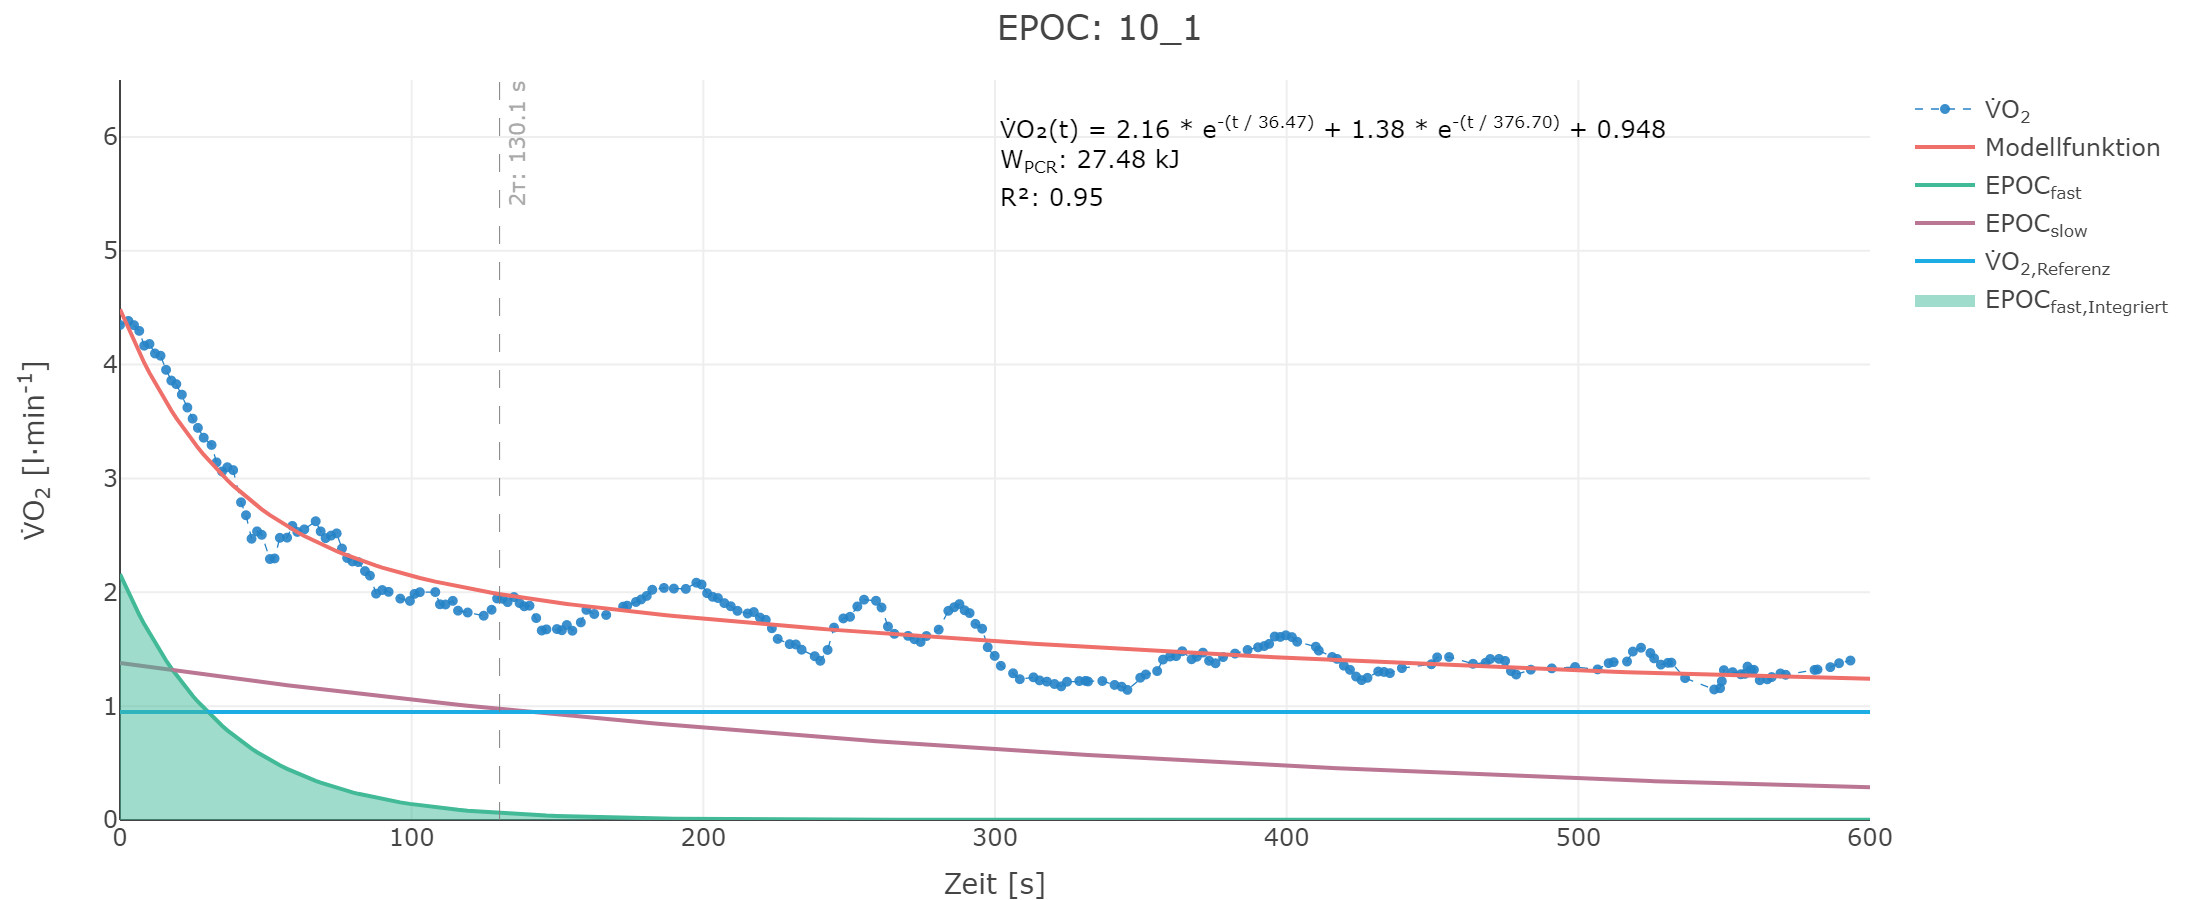
\includegraphics[width=11.45833in,height=4.6875in]{images/10_1.png}

\subsubsection{Test 2}

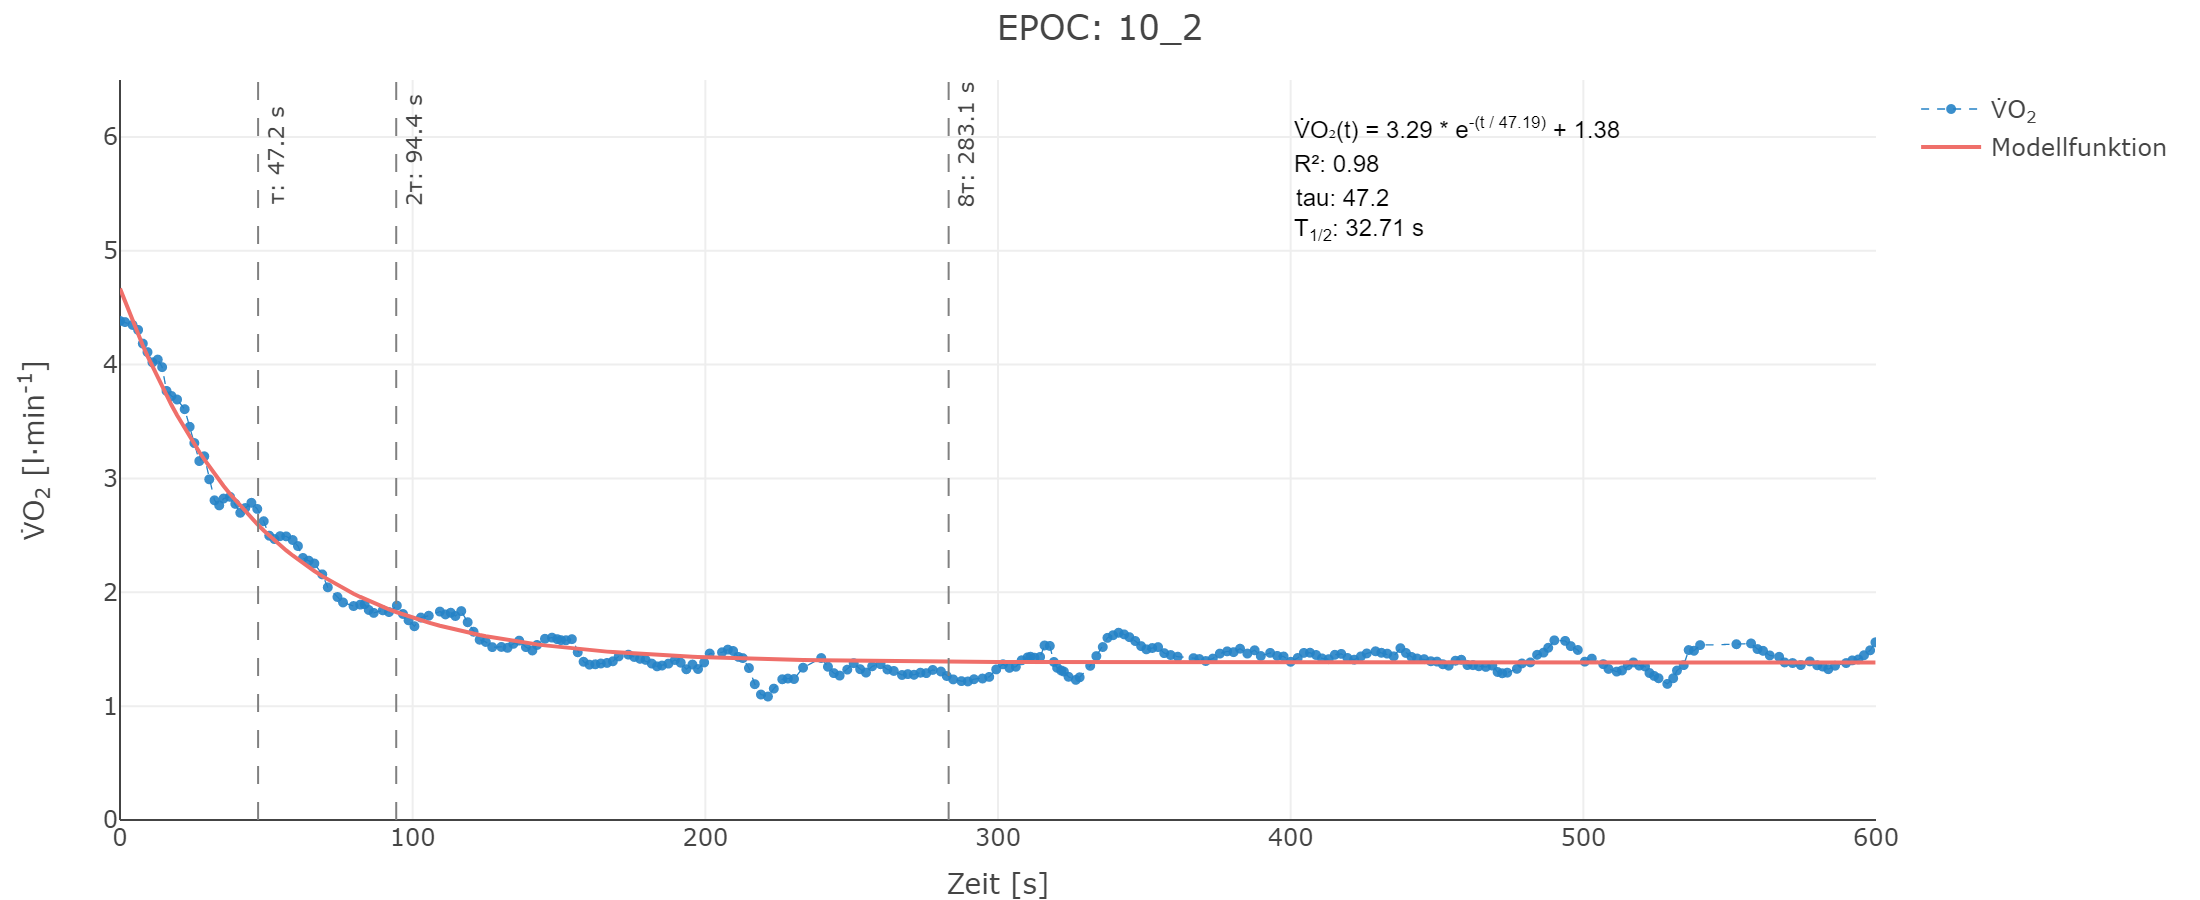
\includegraphics[width=11.45833in,height=4.6875in]{images/10_2_tau.png}
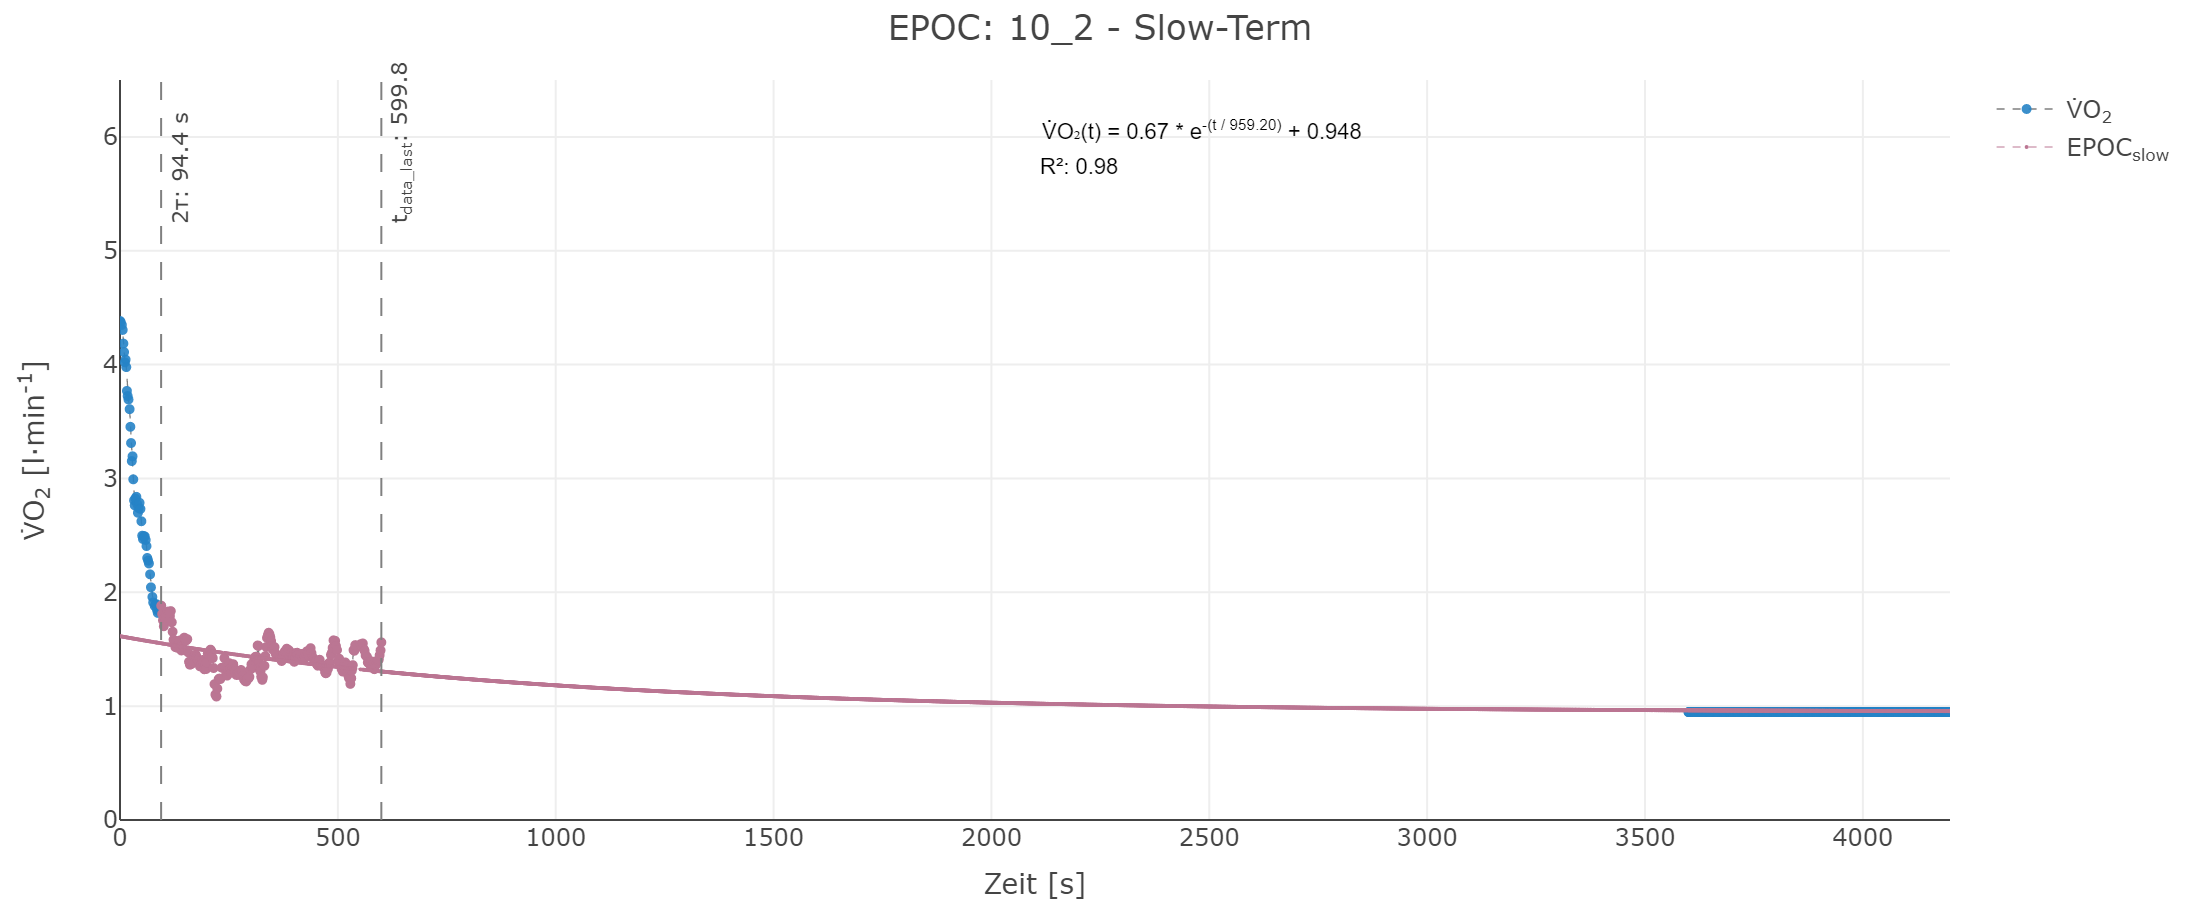
\includegraphics[width=11.45833in,height=4.6875in]{images/10_2_slow.png}
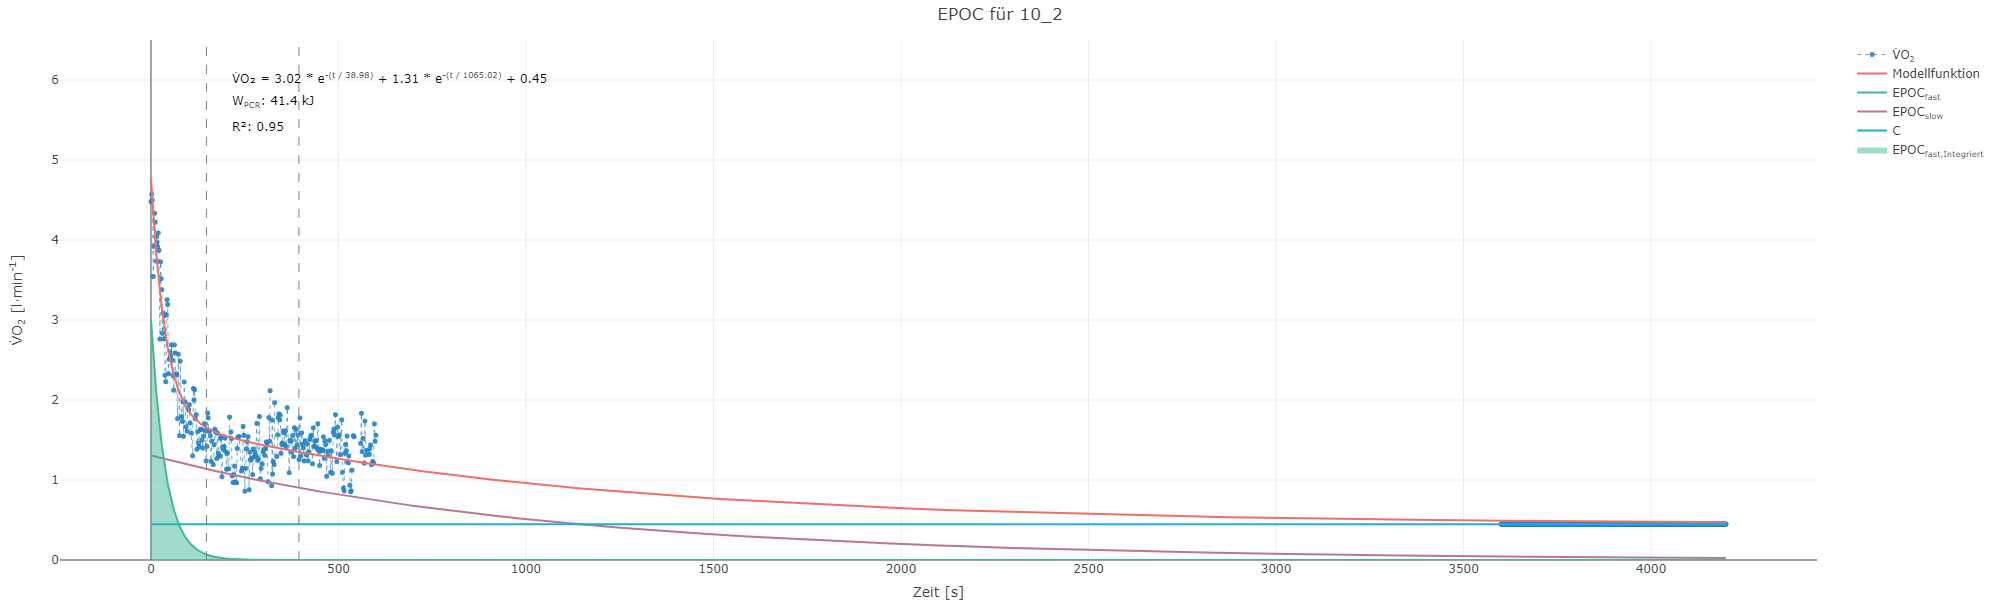
\includegraphics[width=11.45833in,height=4.6875in]{images/10_2.png}

\subsubsection{Test 3}

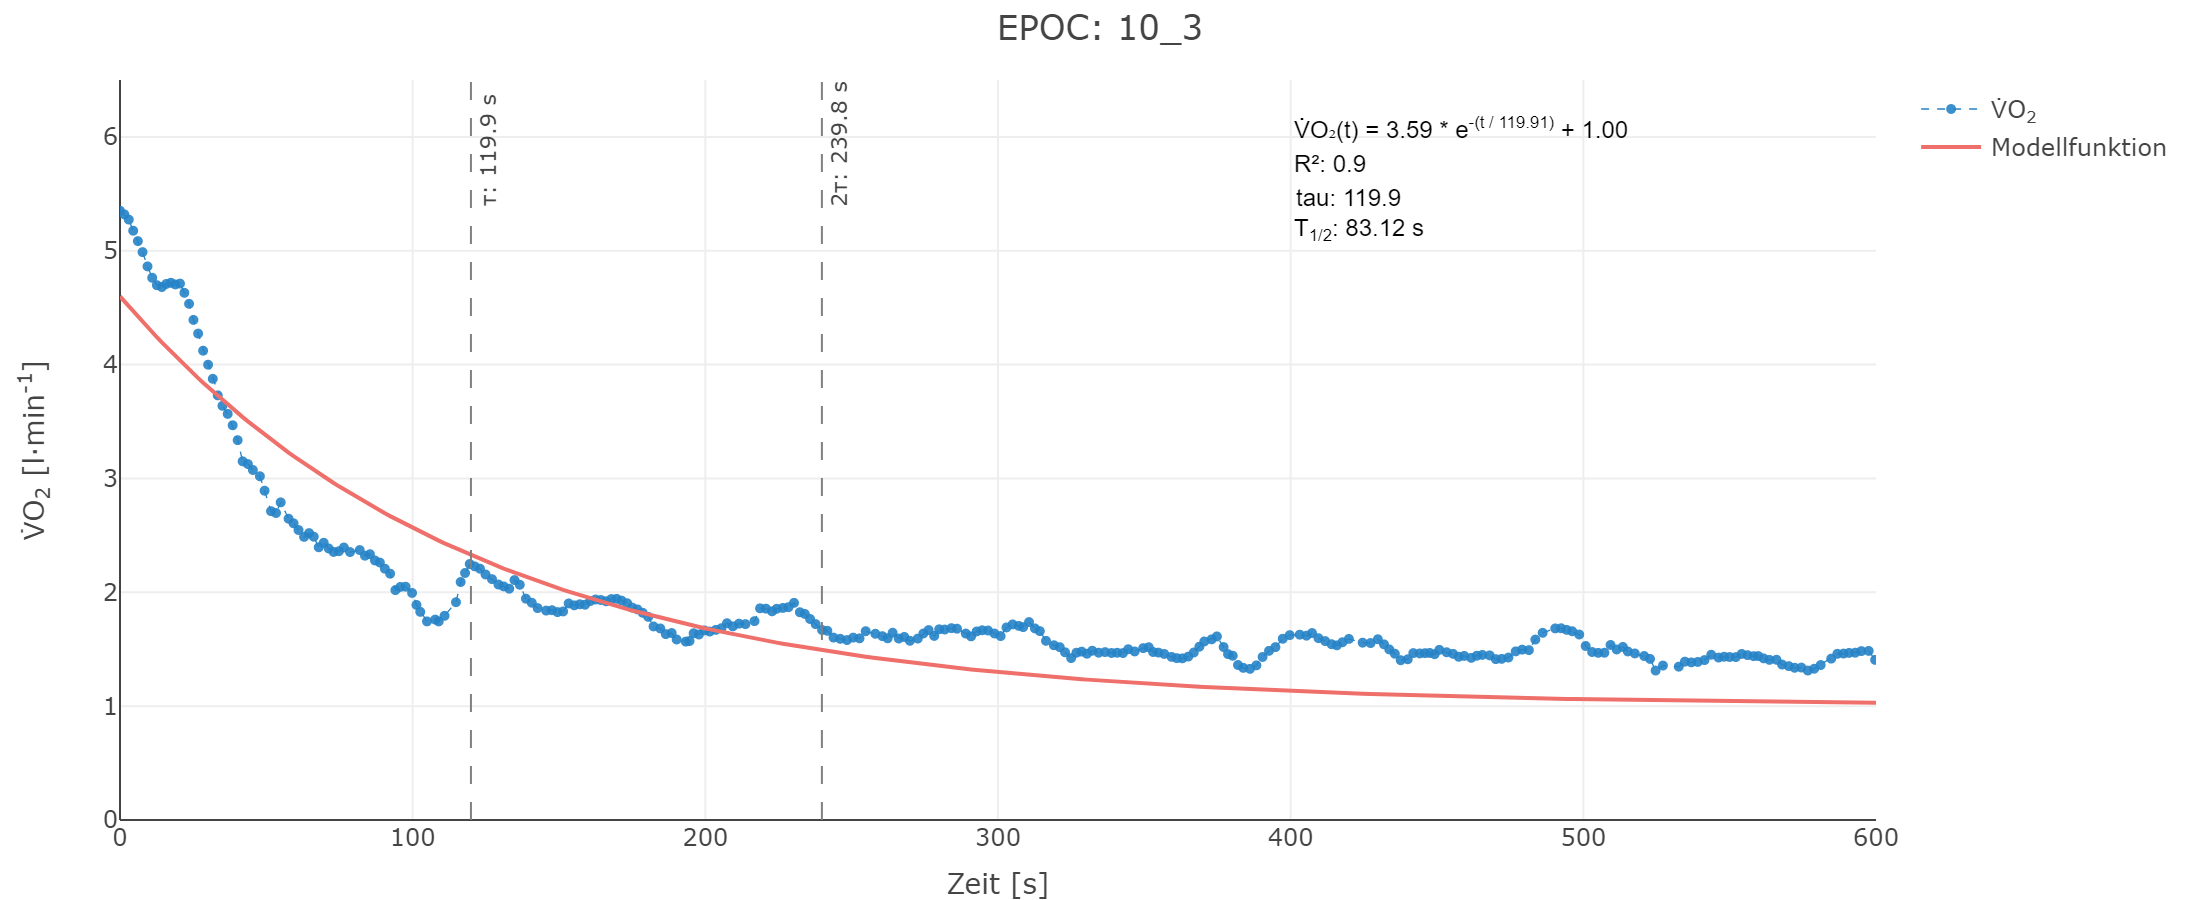
\includegraphics[width=11.45833in,height=4.6875in]{images/10_3_tau.png}
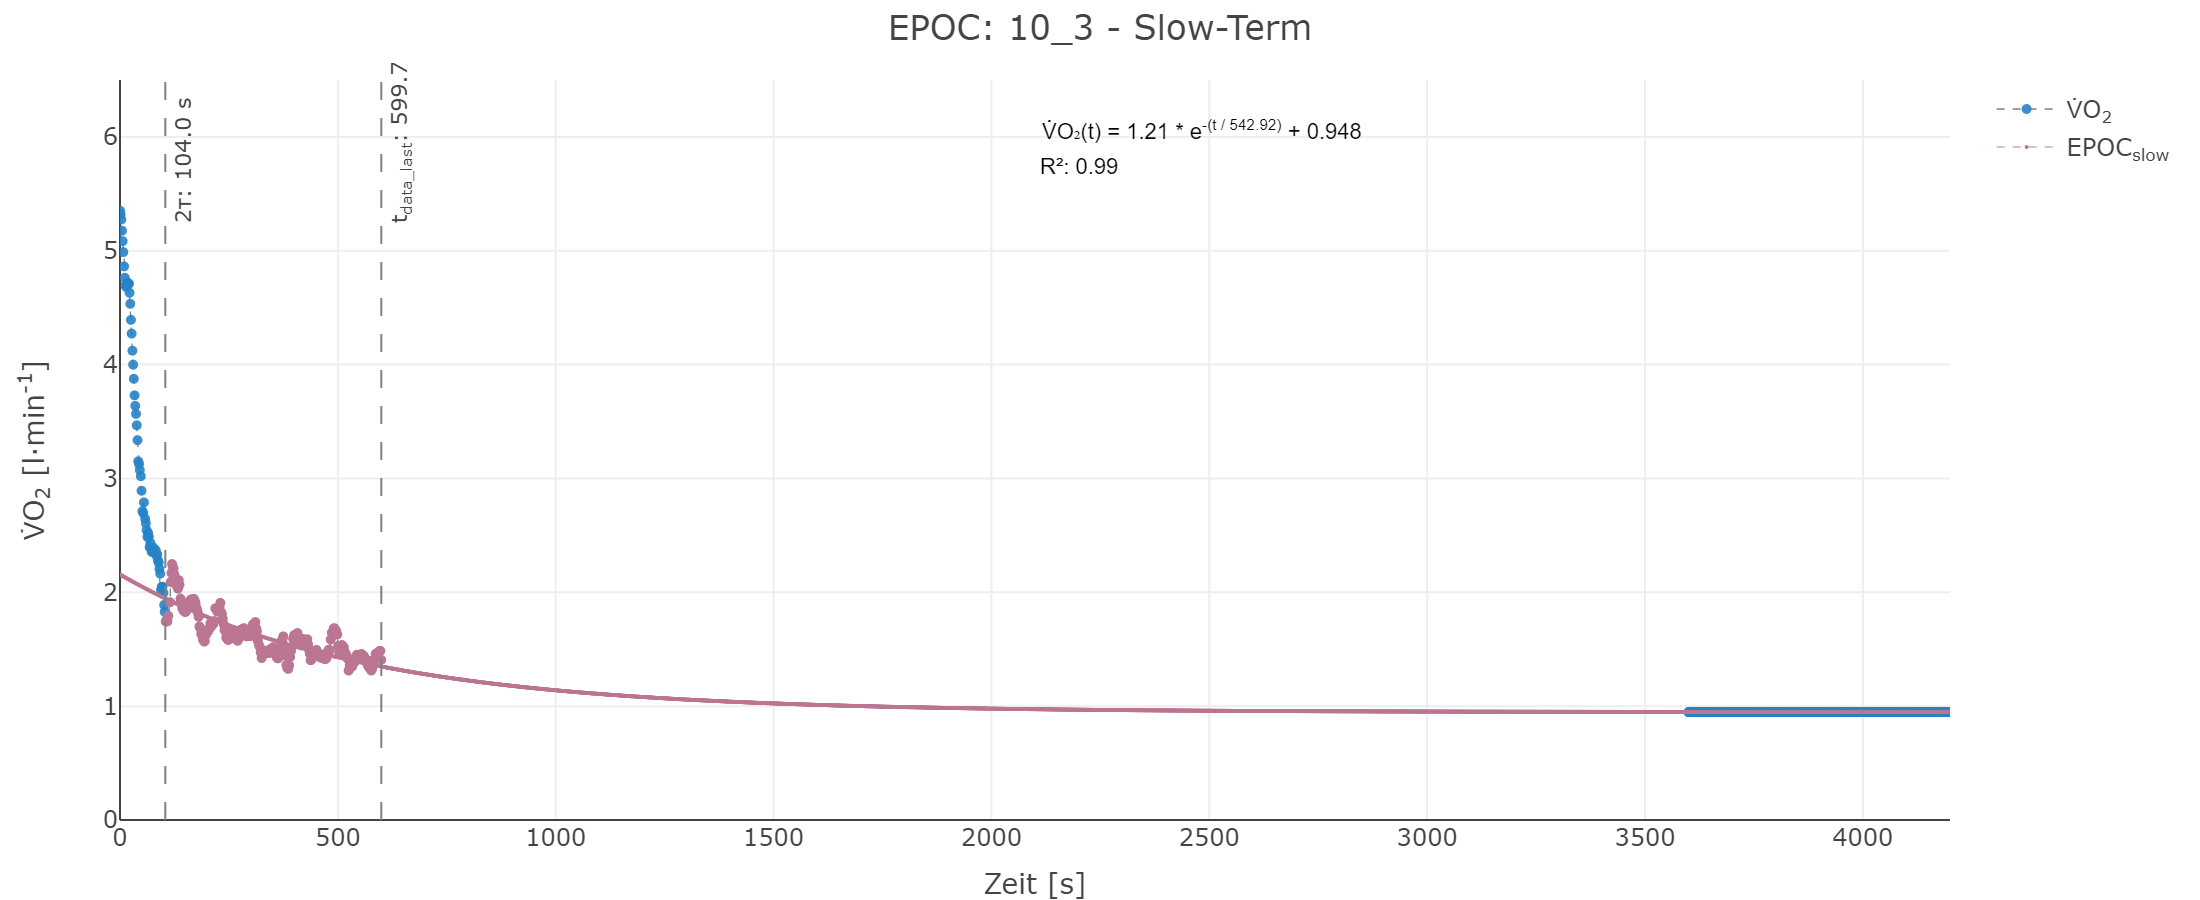
\includegraphics[width=11.45833in,height=4.6875in]{images/10_3_slow.png}
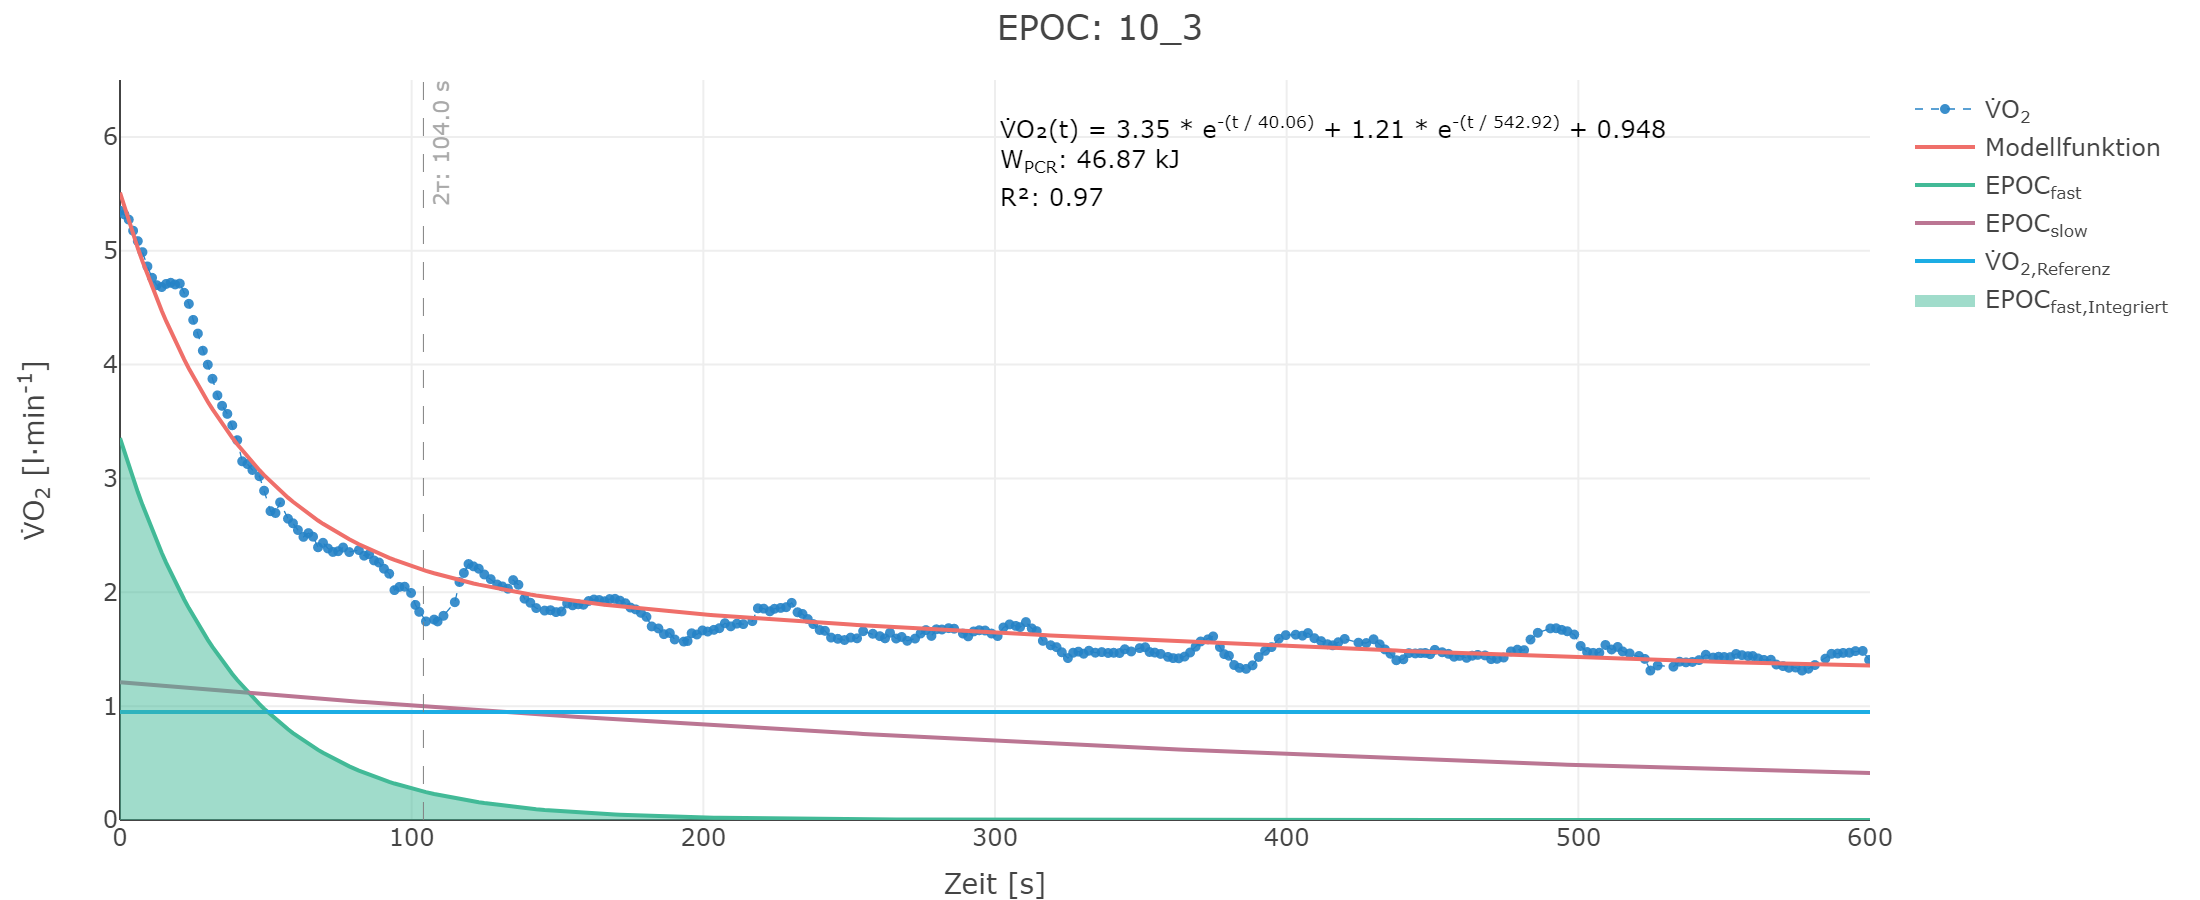
\includegraphics[width=11.45833in,height=4.6875in]{images/10_3.png}

\subsubsection{Test 4}

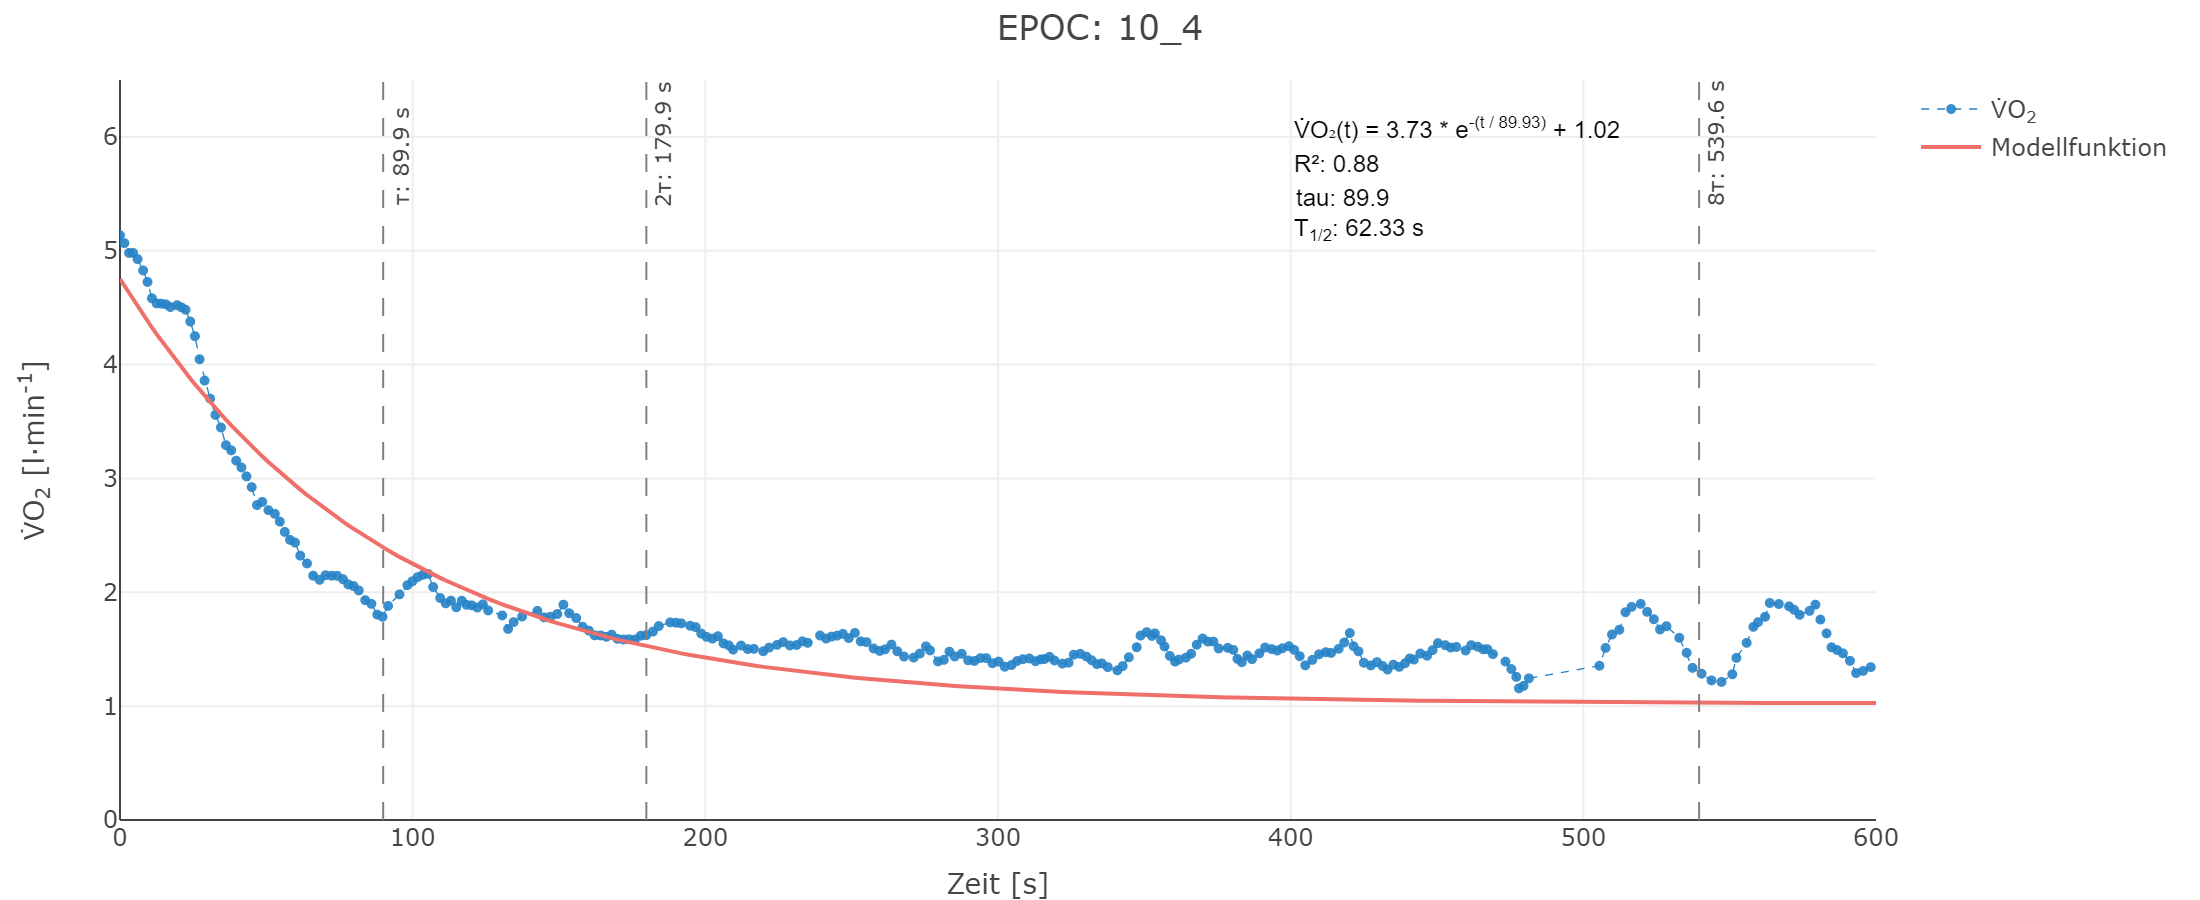
\includegraphics[width=11.45833in,height=4.6875in]{images/10_4_tau.png}
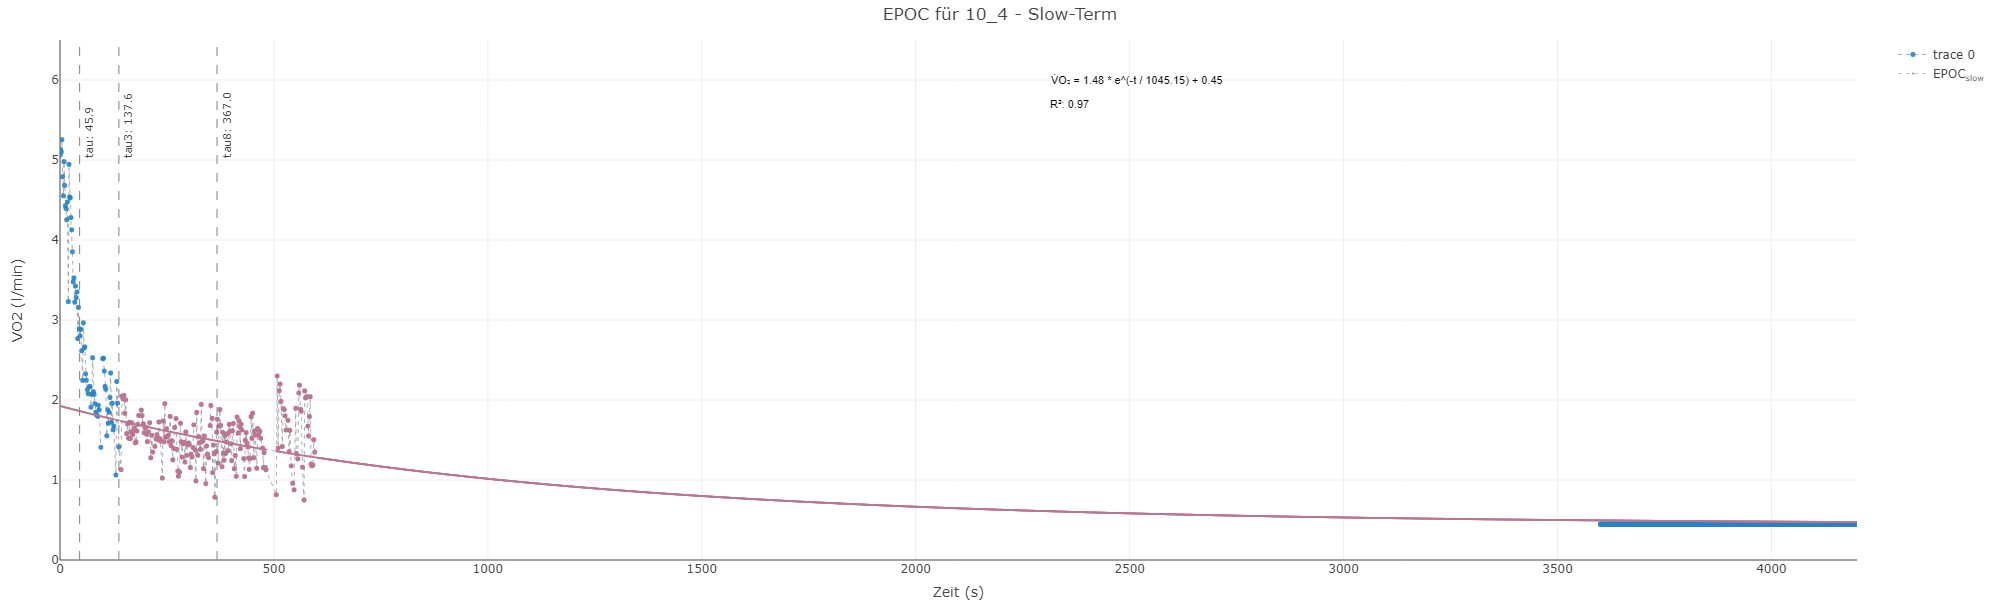
\includegraphics[width=11.45833in,height=4.6875in]{images/10_4_slow.png}
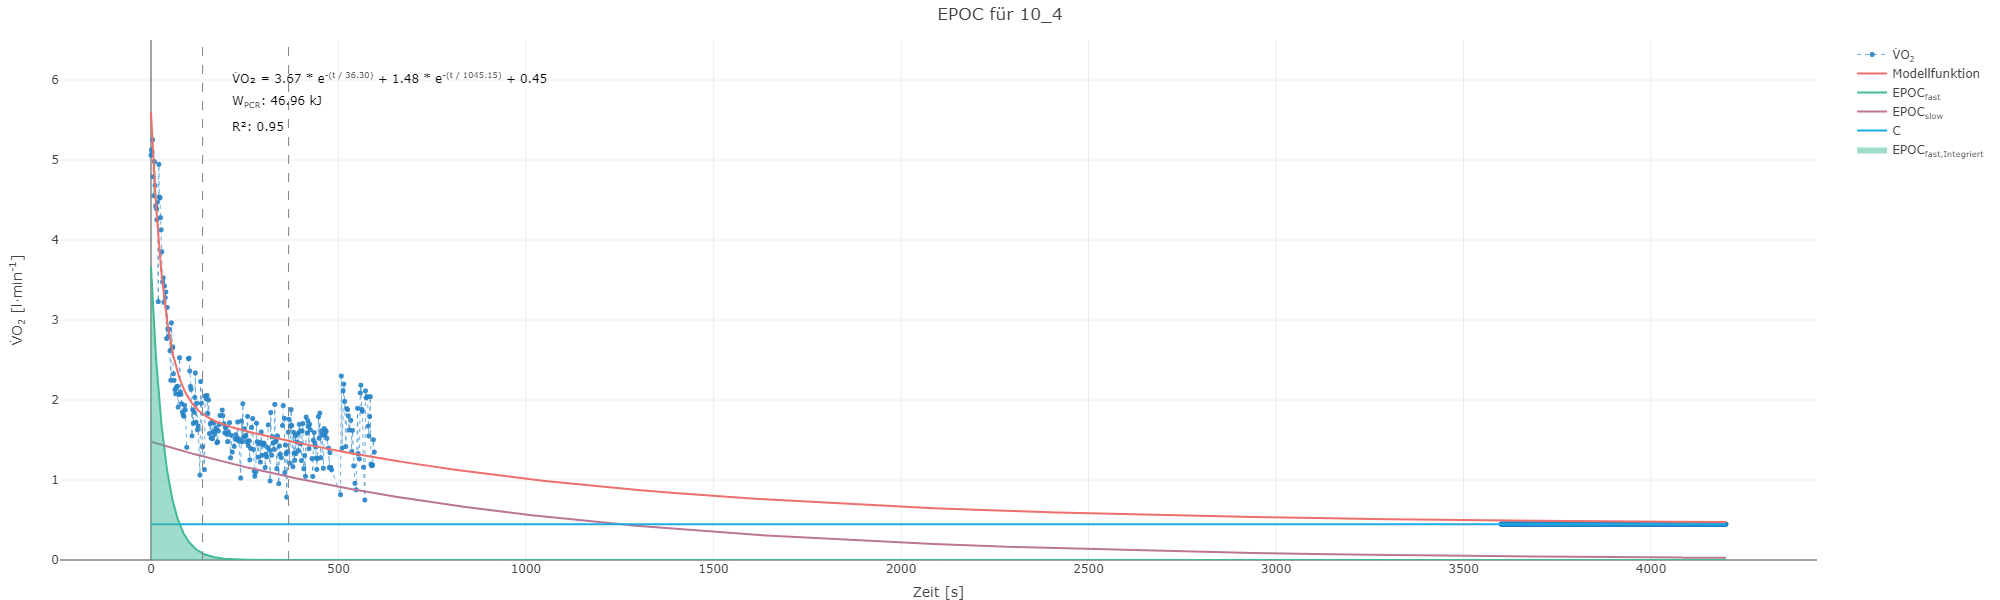
\includegraphics[width=11.45833in,height=4.6875in]{images/10_4.png}

\subsubsection{Test 5}

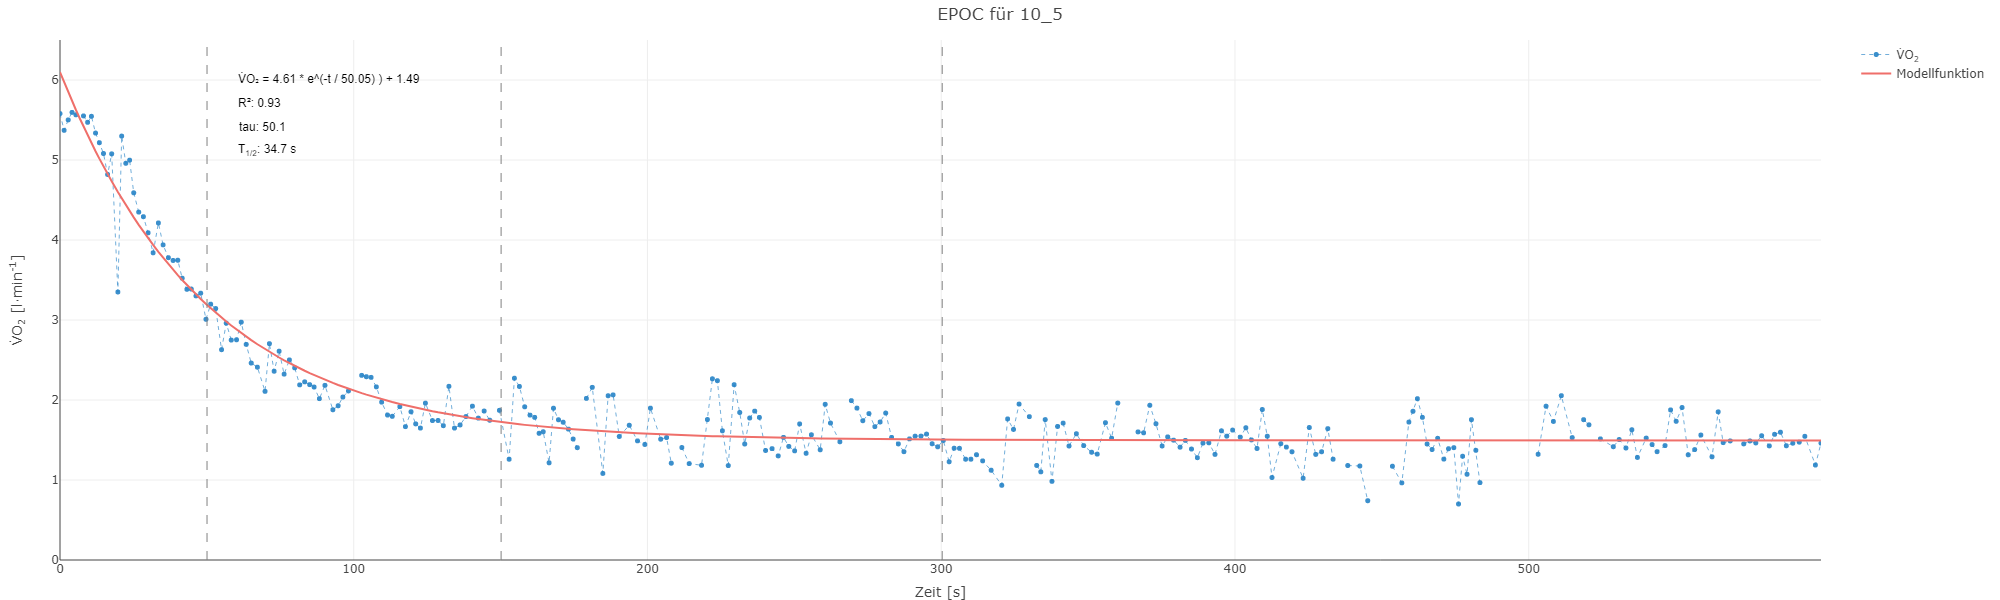
\includegraphics[width=11.45833in,height=4.6875in]{images/10_5_tau.png}
\includegraphics[width=11.45833in,height=4.6875in]{images/10_5_slow.png}
\includegraphics[width=11.45833in,height=4.6875in]{images/10_5.png}

\subsubsection{Test 6}

\includegraphics[width=11.45833in,height=4.6875in]{images/10_6_tau.png}
\includegraphics[width=11.45833in,height=4.6875in]{images/10_6_slow.png}
\includegraphics[width=11.45833in,height=4.6875in]{images/10_6.png}

\subsection{Proband 13}

\subsubsection{Test 1}

\includegraphics[width=11.45833in,height=4.6875in]{images/13_1_tau.png}
\includegraphics[width=11.45833in,height=4.6875in]{images/13_1_slow.png}
\includegraphics[width=11.45833in,height=4.6875in]{images/13_1.png}

\subsubsection{Test 2}

\includegraphics[width=11.45833in,height=4.6875in]{images/13_2_tau.png}
\includegraphics[width=11.45833in,height=4.6875in]{images/13_2_slow.png}
\includegraphics[width=11.45833in,height=4.6875in]{images/13_2.png}

\subsubsection{Test 3}

\includegraphics[width=11.45833in,height=4.6875in]{images/13_3_tau.png}
\includegraphics[width=11.45833in,height=4.6875in]{images/13_3_slow.png}
\includegraphics[width=11.45833in,height=4.6875in]{images/13_3.png}

\subsubsection{Test 4}

\includegraphics[width=11.45833in,height=4.6875in]{images/13_4_tau.png}
\includegraphics[width=11.45833in,height=4.6875in]{images/13_4_slow.png}
\includegraphics[width=11.45833in,height=4.6875in]{images/13_4.png}

\subsubsection{Test 5}

\includegraphics[width=11.45833in,height=4.6875in]{images/13_5_tau.png}
\includegraphics[width=11.45833in,height=4.6875in]{images/13_5_slow.png}
\includegraphics[width=11.45833in,height=4.6875in]{images/13_5.png}

\subsubsection{Test 6}

\includegraphics[width=11.45833in,height=4.6875in]{images/13_6_tau.png}
\includegraphics[width=11.45833in,height=4.6875in]{images/13_6_slow.png}
\includegraphics[width=11.45833in,height=4.6875in]{images/13_6.png}

\subsection{Proband 15}

\subsubsection{Test 1}

\includegraphics[width=11.45833in,height=4.6875in]{images/15_1_tau.png}
\includegraphics[width=11.45833in,height=4.6875in]{images/15_1_slow.png}
\includegraphics[width=11.45833in,height=4.6875in]{images/15_1.png}

\subsubsection{Test 2}

\includegraphics[width=11.45833in,height=4.6875in]{images/15_2_tau.png}
\includegraphics[width=11.45833in,height=4.6875in]{images/15_2_slow.png}
\includegraphics[width=11.45833in,height=4.6875in]{images/15_2.png}

\subsubsection{Test 3}

\includegraphics[width=11.45833in,height=4.6875in]{images/15_3_tau.png}
\includegraphics[width=11.45833in,height=4.6875in]{images/15_3_slow.png}
\includegraphics[width=11.45833in,height=4.6875in]{images/15_3.png}

\subsubsection{Test 4}

\includegraphics[width=11.45833in,height=4.6875in]{images/15_4_tau.png}
\includegraphics[width=11.45833in,height=4.6875in]{images/15_4_slow.png}
\includegraphics[width=11.45833in,height=4.6875in]{images/15_4.png}

\subsubsection{Test 5}

\includegraphics[width=11.45833in,height=4.6875in]{images/15_5_tau.png}
\includegraphics[width=11.45833in,height=4.6875in]{images/15_5_slow.png}
\includegraphics[width=11.45833in,height=4.6875in]{images/15_5.png}

\subsubsection{Test 6}

\includegraphics[width=11.45833in,height=4.6875in]{images/15_6_tau.png}
\includegraphics[width=11.45833in,height=4.6875in]{images/15_6_slow.png}
\includegraphics[width=11.45833in,height=4.6875in]{images/15_6.png}

\subsection{Proband 19}

\subsubsection{Test 1}

\includegraphics[width=11.45833in,height=4.6875in]{images/19_1_tau.png}
\includegraphics[width=11.45833in,height=4.6875in]{images/19_1_slow.png}
\includegraphics[width=11.45833in,height=4.6875in]{images/19_1.png}

\subsubsection{Test 2}

\includegraphics[width=11.45833in,height=4.6875in]{images/19_2_tau.png}
\includegraphics[width=11.45833in,height=4.6875in]{images/19_2_slow.png}
\includegraphics[width=11.45833in,height=4.6875in]{images/19_2.png}

\subsubsection{Test 3}

\includegraphics[width=11.45833in,height=4.6875in]{images/19_3_tau.png}
\includegraphics[width=11.45833in,height=4.6875in]{images/19_3_slow.png}
\includegraphics[width=11.45833in,height=4.6875in]{images/19_3.png}

\subsubsection{Test 4}

\includegraphics[width=11.45833in,height=4.6875in]{images/19_4_tau.png}
\includegraphics[width=11.45833in,height=4.6875in]{images/19_4_slow.png}
\includegraphics[width=11.45833in,height=4.6875in]{images/19_4.png}

\subsubsection{Test 5}

\includegraphics[width=11.45833in,height=4.6875in]{images/19_5_tau.png}
\includegraphics[width=11.45833in,height=4.6875in]{images/19_5_slow.png}
\includegraphics[width=11.45833in,height=4.6875in]{images/19_5.png}

\subsubsection{Test 6}

\includegraphics[width=11.45833in,height=4.6875in]{images/19_6_tau.png}
\includegraphics[width=11.45833in,height=4.6875in]{images/19_6_slow.png}
\includegraphics[width=11.45833in,height=4.6875in]{images/19_6.png}

\subsection{Proband 20}

\subsubsection{Test 1}

\includegraphics[width=11.45833in,height=4.6875in]{images/20_1_tau.png}
\includegraphics[width=11.45833in,height=4.6875in]{images/20_1_slow.png}
\includegraphics[width=11.45833in,height=4.6875in]{images/20_1.png}

\subsubsection{Test 2}

\includegraphics[width=11.45833in,height=4.6875in]{images/20_2_tau.png}
\includegraphics[width=11.45833in,height=4.6875in]{images/20_2_slow.png}
\includegraphics[width=11.45833in,height=4.6875in]{images/20_2.png}

\subsubsection{Test 3}

\includegraphics[width=11.45833in,height=4.6875in]{images/20_3_tau.png}
\includegraphics[width=11.45833in,height=4.6875in]{images/20_3_slow.png}
\includegraphics[width=11.45833in,height=4.6875in]{images/20_3.png}

\subsubsection{Test 4}

\includegraphics[width=11.45833in,height=4.6875in]{images/20_4_tau.png}
\includegraphics[width=11.45833in,height=4.6875in]{images/20_4_slow.png}
\includegraphics[width=11.45833in,height=4.6875in]{images/20_4.png}

\subsubsection{Test 5}

\includegraphics[width=11.45833in,height=4.6875in]{images/20_5_tau.png}
\includegraphics[width=11.45833in,height=4.6875in]{images/20_5_slow.png}
\includegraphics[width=11.45833in,height=4.6875in]{images/20_5.png}

\subsubsection{Test 6}

\includegraphics[width=11.45833in,height=4.6875in]{images/20_6_tau.png}
\includegraphics[width=11.45833in,height=4.6875in]{images/20_6_slow.png}
\includegraphics[width=11.45833in,height=4.6875in]{images/20_6.png}

\subsection{Proband 22}

\subsubsection{Test 1}

\includegraphics[width=11.45833in,height=4.6875in]{images/22_1_tau.png}
\includegraphics[width=11.45833in,height=4.6875in]{images/22_1_slow.png}
\includegraphics[width=11.45833in,height=4.6875in]{images/22_1.png}

\subsubsection{Test 2}

\includegraphics[width=11.45833in,height=4.6875in]{images/22_2_tau.png}
\includegraphics[width=11.45833in,height=4.6875in]{images/22_2_slow.png}
\includegraphics[width=11.45833in,height=4.6875in]{images/22_2.png}

\subsubsection{Test 3}

\includegraphics[width=11.45833in,height=4.6875in]{images/22_3_tau.png}
\includegraphics[width=11.45833in,height=4.6875in]{images/22_3_slow.png}
\includegraphics[width=11.45833in,height=4.6875in]{images/22_3.png}

\subsubsection{Test 4}

\includegraphics[width=11.45833in,height=4.6875in]{images/22_4_tau.png}
\includegraphics[width=11.45833in,height=4.6875in]{images/22_4_slow.png}
\includegraphics[width=11.45833in,height=4.6875in]{images/22_4.png}

\subsubsection{Test 5}

\includegraphics[width=11.45833in,height=4.6875in]{images/22_5_tau.png}
\includegraphics[width=11.45833in,height=4.6875in]{images/22_5_slow.png}
\includegraphics[width=11.45833in,height=4.6875in]{images/22_5.png}

\subsubsection{Test 6}

\includegraphics[width=11.45833in,height=4.6875in]{images/22_6_tau.png}
\includegraphics[width=11.45833in,height=4.6875in]{images/22_6_slow.png}
\includegraphics[width=11.45833in,height=4.6875in]{images/22_6.png}

\subsection{Proband 23}

\subsubsection{Test 1}

\includegraphics[width=11.45833in,height=4.6875in]{images/23_1_tau.png}
\includegraphics[width=11.45833in,height=4.6875in]{images/23_1_slow.png}
\includegraphics[width=11.45833in,height=4.6875in]{images/23_1.png}

\subsubsection{Test 2}

\includegraphics[width=11.45833in,height=4.6875in]{images/23_2_tau.png}
\includegraphics[width=11.45833in,height=4.6875in]{images/23_2_slow.png}
\includegraphics[width=11.45833in,height=4.6875in]{images/23_2.png}

\subsubsection{Test 3}

\includegraphics[width=11.45833in,height=4.6875in]{images/23_3_tau.png}
\includegraphics[width=11.45833in,height=4.6875in]{images/23_3_slow.png}
\includegraphics[width=11.45833in,height=4.6875in]{images/23_3.png}

\subsubsection{Test 4}

\includegraphics[width=11.45833in,height=4.6875in]{images/23_4_tau.png}
\includegraphics[width=11.45833in,height=4.6875in]{images/23_4_slow.png}
\includegraphics[width=11.45833in,height=4.6875in]{images/23_4.png}

\subsubsection{Test 5}

\includegraphics[width=11.45833in,height=4.6875in]{images/23_5_tau.png}
\includegraphics[width=11.45833in,height=4.6875in]{images/23_5_slow.png}
\includegraphics[width=11.45833in,height=4.6875in]{images/23_5.png}

\subsubsection{Test 6}

\includegraphics[width=11.45833in,height=4.6875in]{images/23_6_tau.png}
\includegraphics[width=11.45833in,height=4.6875in]{images/23_6_slow.png}
\includegraphics[width=11.45833in,height=4.6875in]{images/23_6.png}

\section{Quellenverzeichnis}\label{quellenverzeichnis}

\phantomsection\label{refs}
\begin{CSLReferences}{1}{0}
\bibitem[\citeproctext]{ref-Bangsbo1993}
Bangsbo, J., Johansen, L., Quistorff, B., \& Saltin, B. (1993). {NMR and
analytic biochemical evaluation of CrP and nucleotides in the human calf
during muscle contraction}. \emph{Journal of Applied Physiology},
\emph{74}(4), 2034--2039.
\url{https://doi.org/10.1152/jappl.1993.74.4.2034}

\bibitem[\citeproctext]{ref-Beneke2004}
Beneke, R., Beyer, T., Jachner, C., Erasmus, J., \& Hütler, M. (2004).
{Energetics of karate kumite.} \emph{European journal of applied
physiology}, \emph{92}(4-5), 518--523.
\url{https://doi.org/10.1007/s00421-004-1073-x}

\bibitem[\citeproctext]{ref-Beneke2002}
Beneke, R., Pollmann, C., Bleif, I., Leithäuser, R. M., \& Hütler, M.
(2002). {How anaerobic is the Wingate Anaerobic Test for humans ?}
\emph{European Journal of Applied Physiology}, \emph{87}, 388--392.
\url{https://doi.org/10.1007/s00421-002-0622-4}

\bibitem[\citeproctext]{ref-Berg1947}
Berg, W. E. (1947). {Individual differences in respiratory gas exchange
during recovery from moderate exercise.} \emph{The American journal of
physiology}, \emph{149}(3), 597--610.
\url{https://doi.org/10.1152/ajplegacy.1947.149.3.597}

\bibitem[\citeproctext]{ref-Bogdanis1996}
Bogdanis, G. C., Nevill, M. E., Boobis, L. H., \& Lakomy, H. K. (1996).
{Contribution of phosphocreatine and aerobic metabolism to energy supply
during repeated sprint exercise.} \emph{Journal of applied physiology
(Bethesda, Md. : 1985)}, \emph{80}(3), 876--884.
\url{https://doi.org/10.1152/jappl.1996.80.3.876}

\bibitem[\citeproctext]{ref-Brooks2004}
Brooks, G. A., Fahey, T. D., \& Baldwin, K. M. (2004). \emph{{Exercise
Physiology: Human Bioenergetics and Its Applications}} (4. Edition, S.
928). McGraw-Hill Education Ltd.

\bibitem[\citeproctext]{ref-DeMoor1954}
DeMoor, J. C. (1954). {Individual differences in oxygen debt curves
related to mechanical efficiency and sex.} \emph{Journal of applied
physiology}, \emph{6}(8), 460--466.
\url{https://doi.org/10.1152/jappl.1954.6.8.460}

\bibitem[\citeproctext]{ref-DiPrampero1971}
Di Prampero, P. E. (1971). {The alactacid oxygen debt: Its power
capacity and efficiency}. In \emph{Muscle Metabolism During Exercise}
(S. 371--382). Plenum Press.

\bibitem[\citeproctext]{ref-DiPrampero1981}
Di Prampero, P. E. (1981). {Energetics of Muscular Exercise}.
\emph{Review of physiology, biochemistry and pharmacology}, \emph{89},
143--222.

\bibitem[\citeproctext]{ref-DiPrampero1970}
Di Prampero, P. E., Davies, C. T., Cerretelli, P., \& Margaria, R.
(1970). {An analysis of O2 debt contracted in submaximal exercise.}
\emph{Journal of applied physiology}, \emph{29}(5), 547--551.
\url{https://doi.org/10.1152/jappl.1970.29.5.547}

\bibitem[\citeproctext]{ref-Dunst2023a}
Dunst, A. K., Hesse, C., Ueberschär, O., \& Holmberg, H. C. (2023). {A
Novel Approach to the Determination of Time- and Fatigue-Dependent
Efficiency during Maximal Cycling Sprints}. \emph{Sports}, \emph{11}(2).
\url{https://doi.org/10.3390/sports11020029}

\bibitem[\citeproctext]{ref-Dunst2023b}
Dunst, A. K., Manunzio, C., Feldmann, A., \& Hesse, C. (2023).
{Applications of near-infrared spectroscopy in {„anaerobic``}
diagnostics - SmO2 kinetics reflect PCr dephosphorylation and correlate
with maximal lactate accumulation and maximal pedalling rate}.
\emph{Biology of Sport}, \emph{40}(4), 1019--1031.
\url{https://doi.org/10.5114/BIOLSPORT.2023.122481}

\bibitem[\citeproctext]{ref-Francescato2003}
Francescato, M. P., Cettolo, V., \& Di Prampero, P. E. (2003).
{Relationships between mechanical power, O2 consumption, O2 deficit and
high-energy phosphates during calf exercise in humans}. \emph{Pflugers
Archiv European Journal of Physiology}, \emph{445}(5), 622--628.
\url{https://doi.org/10.1007/s00424-002-0992-9}

\bibitem[\citeproctext]{ref-Gaitanos1993}
Gaitanos, G. C., Williams, C., Boobis, L. H., \& Brooks, S. (1993).
{Human muscle metabolism during intermittent maximal exercise.}
\emph{Journal of applied physiology}, \emph{75}(2), 712--719.
\url{https://doi.org/10.1152/jappl.1993.75.2.712}

\bibitem[\citeproctext]{ref-Harris1974}
Harris, R. C., Hultman, E., \& Nordesjö, L. O. (1974). {Glycogen,
glycolytic intermediates and high-energy phosphates determined in biopsy
samples of musculus quadriceps femoris of man at rest. Methods and
variance of values}. \emph{Scandinavian Journal of Clinical and
Laboratory Investigation}, \emph{33}(2), 109--120.
\url{https://doi.org/10.1080/00365517409082477}

\bibitem[\citeproctext]{ref-Heck2006}
Heck, H. (2006). {Muskul{ä}rer Energiestoffwechsel und sportliche
Aktivit{ä}t}. \emph{Blickpunkt der Mann}, \emph{4}(4), 23--28.

\bibitem[\citeproctext]{ref-Henry1951}
Henry, F. M. (1951). {Aerobic oxygen consumption and alactic debt in
muscular work.} \emph{Journal of applied physiology}, \emph{3}(7),
427--438. \url{https://doi.org/10.1152/jappl.1951.3.7.427}

\bibitem[\citeproctext]{ref-Henry1950a}
Henry, F. M., \& Berg, W. E. (1950). {Physiological and performance
changes in athletic conditioning.} \emph{Journal of applied physiology},
\emph{3}(2), 103--111. \url{https://doi.org/10.1152/jappl.1950.3.2.103}

\bibitem[\citeproctext]{ref-Henry1950}
Henry, F. M., \& DeMoor, J. C. (1950). {Metabolic efficiency of exercise
in relation to work load at constant speed.} \emph{Journal of applied
physiology}, \emph{2}(9), 481--487.
\url{https://doi.org/10.1152/jappl.1950.2.9.481}

\bibitem[\citeproctext]{ref-Henry1956}
Henry, F. M., \& DeMoor, J. C. (1956). {Lactic and alactic oxygen
consumption in moderate exercise of graded intensity}. \emph{Journal of
applied physiology}, \emph{8}(6), 608--614.
\url{https://doi.org/10.1152/jappl.1956.8.6.608}

\bibitem[\citeproctext]{ref-Hill1924}
Hill, A. V., Long, C. N. H., \& Lupton, H. (1924). {Muscular exercise,
lactic acid, and the supply and utilisation of oxygen}.
\emph{Proceedings of the Royal Society of London. Series B, Containing
Papers of a Biological Character}, \emph{96}(679), 438--475.
\url{https://doi.org/10.1098/rspb.1924.0037}

\bibitem[\citeproctext]{ref-Horn2021}
Horn, F., Blaeschke, F., Trugenberger, K., Gröll, M., Polzer, C.,
Lechner, K., \& Anderson, J. M. (2021). \emph{{Biochemie des Menschen :
das Lehrbuch f{ü}r das Medizinstudium}} (8. Edition, S. 790). Georg
Thieme Verlag. \url{https://doi.org/10.1055/b000000082}

\bibitem[\citeproctext]{ref-Hultman1967}
Hultman, E., Bergström, J., \& Anderson, N. M. (1967). {Breakdown and
resynthesis of phosphorylcreatine and adenosine triphosphate in
connection with muscular work in man}. \emph{Scandinavian Journal of
Clinical and Laboratory Investigation}, \emph{19}(1), 56--66.
\url{https://doi.org/10.3109/00365516709093481}

\bibitem[\citeproctext]{ref-Karlsson1971}
Karlsson, J. (1971).
\href{https://www.ncbi.nlm.nih.gov/pubmed/5549478}{{Lactate and
phosphagen concentrations in working muscle of man with special
reference to oxygen deficit at the onset of work.}} \emph{Acta
physiologica Scandinavica. Supplementum}, \emph{358}, 1--72.

\bibitem[\citeproctext]{ref-Katch1973}
Katch, V. L. (1973). {Kinetics of oxygen uptake and recovery for
supramaximal work of short duration}. \emph{Internationale Zeitschrift
f{ü}r Angewandte Physiologie Einschlie{ß}lich Arbeitsphysiologie},
\emph{31}(3), 197--207. \url{https://doi.org/10.1007/BF00697599}

\bibitem[\citeproctext]{ref-Keul1972}
Keul, J., Doll, E., \& Keppler, D. (1972). \emph{{Energy Metabolism of
Human Muscle}} (E. Jokl \& Ky. Lexington, Hrsg.; Bd. 7, S. 312).
University Park Press.

\bibitem[\citeproctext]{ref-Knuttgen1973}
Knuttgen, H. G., \& Saltin, B. (1973). {Oxygen Uptake, Muscle
High‐Energy Phosphates, and Lactate in Exercise under Acute Hypoxic
Conditions in Man}. \emph{Acta Physiologica Scandinavica}, \emph{87}(3),
368--376. \url{https://doi.org/10.1111/j.1748-1716.1973.tb05401.x}

\bibitem[\citeproctext]{ref-Langley2024}
Langley, J. O., Ng, S. C., Todd, E. E., \& Porter, M. S. (2024).
{VLamax: determining the optimal test duration for maximal lactate
formation rate during all-out sprint cycle ergometry}. \emph{European
Journal of Applied Physiology}.
\url{https://doi.org/10.1007/s00421-024-05456-9}

\bibitem[\citeproctext]{ref-DeMarees2003}
Marées, H. de. (2003). \emph{{Sportphysiologie}} (H. Heck \& U. Bartmus,
Hrsg.; 9. Edition, S. 799). Sportverlag Strauss.

\bibitem[\citeproctext]{ref-Margaria1972}
Margaria, R. (1972). {The sources of muscular energy.} \emph{Scientific
American}, \emph{226}(3), 84--91.
\url{https://doi.org/10.1038/scientificamerican0372-84}

\bibitem[\citeproctext]{ref-Margaria1976}
Margaria, R. (1976). \emph{{Biomechanics and energetics of muscular
exercise}} (S. 144). Oxford University Press.

\bibitem[\citeproctext]{ref-Margaria1963}
Margaria, R., Cerretelli, P., Aghemo, P., \& Sassi, G. (1963). {Energy
cost of running.} \emph{Journal of applied physiology}, \emph{18},
367--370. \url{https://doi.org/10.1152/jappl.1963.18.2.367}

\bibitem[\citeproctext]{ref-Margaria1964}
Margaria, R., Cerretelli, P., \& Mangili, F. (1964). {Balance and
Kinetics of Anaerobic Energy Release During Strenuous Exercise in Man}.
\emph{Journal of applied physiology}, \emph{19}, 623--628.
\url{https://doi.org/10.1152/jappl.1964.19.4.623}

\bibitem[\citeproctext]{ref-Margaria1933}
Margaria, R., Edwards, H. T., \& Dill, D. B. (1933). {THE POSSIBLE
MECHANISMS OF CONTRACTING AND PAYING THE OXYGEN DEBT AND THE R{Ô}LE OF
LACTIC ACID IN MUSCULAR CONTRACTION}. \emph{American Journal of
Physiology}, \emph{106}, 689--715.
\url{https://api.semanticscholar.org/CorpusID:30044859}

\bibitem[\citeproctext]{ref-Nelson2012}
Nelson, D. L., \& Cox, M. M. (2012). \emph{{Lehninger Principles of
Biochemistry: 6th Edition}}. Macmillan Learning.
\url{https://books.google.de/books?id=n9e1NAEACAAJ}

\bibitem[\citeproctext]{ref-Oezyener2001}
Özyener, F., Rossiter, H. B., Ward, S. A., \& Whipp, B. J. (2001).
{Influence of exercise intensity on the on- and off-transient kinetics
of pulmonary oxygen uptake in humans.} \emph{The Journal of physiology},
\emph{533}(Pt 3), 891--902.
\url{https://doi.org/10.1111/j.1469-7793.2001.t01-1-00891.x}

\bibitem[\citeproctext]{ref-Parolin2000}
Parolin, M. L., Spriet, L. L., Hultman, E., Hollidge-Horvat, M. G.,
Jones, N. L., \& Heigenhauser, G. J. F. (2000). {Regulation of glycogen
phosphorylase and PDH during exercise in human skeletal muscle during
hypoxia}. \emph{American Journal of Physiology - Endocrinology and
Metabolism}, \emph{278}(3 41-3), 522--534.
\url{https://doi.org/10.1152/ajpendo.2000.278.3.e522}

\bibitem[\citeproctext]{ref-DiPrampero1973}
Prampero, P. E. di, Peeters, L., \& Margaria, R. (1973). {Alactic O2
debt and lactic acid production after exhausting exercise in man}.
\emph{Journal of Applied Physiology}, \emph{5}.

\bibitem[\citeproctext]{ref-Putman1998}
Putman, C. T., Jones, N. L., Hultman, E., Hollidge-Horvat, M. G., Bonen,
A., McConachie, D. R., \& Heigenhauser, G. J. F. (1998). {Effects of
short-term submaximal training in humans on muscle metabolism in
exercise}. \emph{American Journal of Physiology - Endocrinology and
Metabolism}, \emph{275}(1 38-1), 132--139.
\url{https://doi.org/10.1152/ajpendo.1998.275.1.e132}

\bibitem[\citeproctext]{ref-Roberts1978}
Roberts, A. D., \& Morton, A. R. (1978). \emph{{Applied Physiology}}.
\emph{289}, 281--289.

\bibitem[\citeproctext]{ref-Royce1969}
Royce, J. (1969). {Active and passive recovery from maximal aerobic
capacity work}. \emph{Internationale Zeitschrift fur angewandte
Physiologie, einschliesslich Arbeitsphysiologie}, \emph{28}(1), 1--8.
\url{https://doi.org/10.1007/BF00696033}

\bibitem[\citeproctext]{ref-Stegemann1991}
Stegemann, J. (1991). \emph{{Leistungsphysiologie}} (4. Edition, S.
385). Georg Thieme Verlag.

\bibitem[\citeproctext]{ref-Walter1999}
Walter, G., Vandenborne, K., Elliott, M., \& Leigh, J. S. (1999). {In
vivo ATP synthesis rates in single human muscles during high intensity
exercise}. \emph{Journal of Physiology}, \emph{519}(3), 901--910.
\url{https://doi.org/10.1111/j.1469-7793.1999.0901n.x}

\end{CSLReferences}



\end{document}
